\documentclass[12pt,letterpaper]{article}

%%
%% Required packages:
%%
\usepackage{etex}
\usepackage{amsmath}
\usepackage{amssymb}
\usepackage{amstext}
\usepackage{amsthm}
\usepackage{fancyhdr,fancybox}
\usepackage{mathrsfs} % need for \mathscr command
\usepackage{multicol}
\usepackage[normalem]{ulem}
%\usepackage{pictex,pictexplus}
% \usepackage{pictexwd}
\usepackage{rotating}
\usepackage{url}
\usepackage{xfrac}
\usepackage{booktabs}
\usepackage{color,soul}
\usepackage{comment}

\usepackage{hyperref}
\hypersetup{
    colorlinks=true,     % false: boxed links; true: colored links
    linkcolor=blue,      % color of internal links
    citecolor=blue,      % color of links to bibliography
    filecolor=blue,      % color of file links
    urlcolor=blue        % color of external links
}


\usepackage{tikz}
\usetikzlibrary{backgrounds,calc}

%%
%% Common formatting commands
%%
\setlength{\parindent}{0in}
\setlength{\textwidth}{7in}
\setlength{\evensidemargin}{-0.25in}
\setlength{\oddsidemargin}{-0.25in}
\setlength{\parskip}{.5\baselineskip}
\setlength{\topmargin}{-0.5in}
\setlength{\textheight}{9in}

%               Problem and Part
\newcounter{problemnumber}
\newcounter{partnumber}
\newcounter{subpartnumber}
\newcommand{\Problem}{%
  \refstepcounter{problemnumber}%
  \setcounter{partnumber}{0}%
  \setcounter{subpartnumber}{0}%
  \item[\makebox{\hfil\textbf{\theproblemnumber.}\hfil}]%
  }
\newcommand{\InProblem}[2][1.6]{%
  \refstepcounter{problemnumber}%
  \setcounter{partnumber}{0}%
  \setcounter{subpartnumber}{0}%
  \textbf{\theproblemnumber.}\ \ \parbox[t]{#1in}{#2}%
}
\newcommand{\InSmallProblem}[1]{\InProblem[1.05]{#1}}
\newcommand{\NoProblem}[1]{%
  \mbox{\hfil\textbf{#1}\hfil}%
  }
\newcommand{\UnProblem}{%
  \refstepcounter{problemnumber}%
  \setcounter{partnumber}{0}%
  \setcounter{subpartnumber}{0}%
  \mbox{\hfil\textbf{\theproblemnumber.}\hfil}%
  }
\newcommand{\InFlexProblem}[1]{%
  \refstepcounter{problemnumber}%
  \setcounter{partnumber}{0}%
  \setcounter{subpartnumber}{0}%
  \textbf{\theproblemnumber.}\ \ #1%
}
%%  Part:
\newcommand{\Part}{%
  \renewcommand{\thepartnumber}{(\alph{partnumber})}%
  \refstepcounter{partnumber}
  \setcounter{subpartnumber}{0}%
  \item[(\alph{partnumber})]%
}
\newcommand{\InPart}[2][1.75]{%
  \renewcommand{\thepartnumber}{(\alph{partnumber})}%
  \refstepcounter{partnumber}%
  \setcounter{subpartnumber}{0}%
  (\alph{partnumber})\ \ \parbox[t]{#1in}{#2}%
}
\newcommand{\UnPart}{%
  \refstepcounter{partnumber}%
  \renewcommand{\thepartnumber}{(\alph{partnumber})}%
  \setcounter{subpartnumber}{0}%
  (\alph{partnumber})%
}
\newcommand{\InLargePart}[1]{\InPart[3.05]{#1}}
\newcommand{\InFullPart}[1]{\InPart[6.2]{#1}}
\newcommand{\InSmallPart}[1]{\InPart[1.05]{#1}}
%% SubPart:
\newcommand{\SubPart}{%
  \refstepcounter{subpartnumber}%
  \item[(\roman{subpartnumber})]%
  }
\newcommand{\InSubPart}[2][2.25]{%
  \stepcounter{subpartnumber}%
  (\roman{subpartnumber})\ \ \parbox[t]{#1in}{#2}%
}
\newcommand{\InSmallSubPart}[1]{\InSubPart[1.5]{#1}}
\newcommand{\InTinySubPart}[1]{%
  \stepcounter{subpartnumber}%
  (\roman{subpartnumber})\ \ \makebox{#1}%
}
\newcommand{\InMySubPart}[2][2.25]{%
  \stepcounter{subpartnumber}%
  \parbox[t]{#1in}{\makebox[0.3in][l]{(\roman{subpartnumber})}\ \ {#2}}%
}
\newcommand{\TrueFalse}{\textbf{T}\ \ \textbf{F}\ \ }
\newcommand{\TFPart}[1]{% 
  \stepcounter{partnumber}%
  \setcounter{subpartnumber}{0}%
  \item[(\alph{partnumber})] \TrueFalse\parbox[t]{5.5in}{#1}}

\newcommand{\Points}[1]{(#1 points) \ }
\newcommand{\Point}[1]{(#1 point) \ }


%% For Answers:
\newcounter{answernumber}
\newcommand{\Answer}{%
  \refstepcounter{answernumber}%
  \setcounter{partnumber}{0}%
  \setcounter{subpartnumber}{0}%
  \item[\makebox{\hfil\textbf{\theanswernumber.}\hfil}]%
  }


% Setting up the headers for the first page
%\chead{} % will default to what is typed in the file.
\fancyhead[L]{\textsc{Math 22a}}
\fancyhead[R]{\textsc{Fall 2024}}
\fancyfoot[R]{
	\vspace*{\fill}\footnotesize\textcopyright{} \emph{Harvard Math 22a}	
}
\renewcommand{\headrulewidth}{0pt}

%\fancyhead[C]{}
%	\chead{}	
%	\lhead{}
%	\rhead{}
%	\cfoot{}


% Putting copyright on the footer of each page
%\fancypagestyle{secondpage}{
%	\fancyhead[C]{TESTing again} % change this to be blank
%		%\chead{}	
%	\fancyhead[L]{bears} % change this to be blank
%	\fancyhead[R]{dogs} % change this to be blank
%	\fancyfoot[R]{ %keeps the footer the same
%		\vspace*{\fill}\footnotesize\textcopyright{} \emph{Harvard Math 22a}	
%	}
%}
%\renewcommand{\headrulewidth}{0pt}
%\pagestyle{fancy}
\pagestyle{empty}


%\lhead{}
%\rhead{}
%\rfoot{\vspace*{\fill}\footnotesize\textcopyright{} \emph{Harvard Math 22a}}
%\renewcommand{\headrulewidth}{0pt}
%\pagestyle{fancy}




%%
%% Common shortcut commands:
%%
\newcommand{\ds}{\displaystyle}
\newcommand{\sgn}{\operatorname{sgn}}
\renewcommand{\Pr}{\operatorname{P}}
\newcommand{\CPr}[3][{}]{\Pr_{\text{#1}}\left(#2\,|\,#3\right)}

\newcommand{\C}{\mathbb{C}}
\newcommand{\R}{\mathbb{R}}
\newcommand{\Z}{\mathbb{Z}}
\newcommand{\N}{\mathbb{N}}
\newcommand{\Q}{\mathbb{Q}}
\newcommand{\D}{\mathbb{D}}

\newcommand{\rref}{\operatorname{rref}}
\newcommand{\im}{\operatorname{im}}
\newcommand{\rank}{\operatorname{rank}}
\newcommand{\diag}{\operatorname{diag}}
\newcommand{\Span}{\operatorname{span}}
%\renewcommand{\vec}[1]{\mathbf{#1}}
\newcommand{\charpoly}{\mathscr{P}}
\newcommand{\nicefrac}[2]{\sfrac{#1}{#2}} % using xfrac package
\newcommand{\topology}{\mathcal{T}}
\newcommand{\Inn}{\operatorname{Inn}}

\newcommand{\blankbox}[2]{\fbox{\rule{#1}{0in}\rule{0in}{#2}}}

\newenvironment{myindentpar}[1]%
 {\begin{list}{}%
         {\setlength{\leftmargin}{#1}
          \setlength{\rightmargin}{\leftmargin}}%
         \item[]%
 }
 {\end{list}}
\newtheorem{theorem}{Theorem}
\newtheorem*{NStheorem}{Theorem}
\newtheorem{cor}[theorem]{Corollary}
\newtheorem*{claim}{Claim}
\newtheorem{defn}{Definition}

\newenvironment{amatrix}[1]{%
  \left(\begin{array}{@{}*{#1}{c}|c@{}}
}{%
  \end{array}\right)
}

%--------grstep
% For denoting a Gauss' reduction step.
% Use as: \grstep{\rho_1+\rho_3} or \grstep[2\rho_5 \\ 3\rho_6]{\rho_1+\rho_3}
\newcommand{\grstep}[2][\relax]{%
   \ensuremath{\mathrel{
       {\mathop{\longrightarrow}\limits^{#2\mathstrut}_{
                                     \begin{subarray}{l} #1 \end{subarray}}}}}}
\newcommand{\swap}{\leftrightarrow}



\usepackage{logicpuzzle} %Class 01
\usepackage{skak} % for chess! %Class 02
\usetikzlibrary{arrows} %Class 08, 17, 18
\usepackage{wrapfig}    %Class 08, 17, 18

%Class 14, 15, 16, 17, 18
\makeatletter
\renewcommand*\env@matrix[1][*\c@MaxMatrixCols c]{%
        \hskip -\arraycolsep
        \let\@ifnextchar\new@ifnextchar
        \array{#1}}
\makeatother

\def\env@matrix{\hskip -\arraycolsep
        \let\@ifnextchar\new@ifnextchar
        \array{*\c@MaxMatrixCols c}}
%End Class 14, 15,16...

\usepackage{amsfonts,amsmath} % Class 29,30
\newcommand{\norm}[1]{\left\lVert#1\right\rVert} % Class 30


\newcommand{\coursenum}{22a}








\usepackage{fancyhdr}
\lhead{}
\rhead{}
\rfoot{\vspace*{\fill}\footnotesize\textcopyright{} \emph{Harvard Math 22a}}
\renewcommand{\headrulewidth}{0pt}
\pagestyle{fancy}

\title{\Huge \textbf{Math 22a Coursepack}}
\date{}

\begin{document}


\pagenumbering{gobble}

\maketitle


%\begin{center}
%\parbox{6.3in}{\textbf{\Large 
%\begin{framed}
%  There are blank pages and spaces between the questions so that you can do your work and take notes in this book.
%\end{framed}
%}}
%\end{center}



%\vfill

\centerline{\Large Fall 2024}

\vfill
\centerline{\textcopyright{} \emph{Harvard Math 22a}}


\pagebreak

\null


\centerline{\large\textbf{A note on how to use this coursepack:}  }
This coursepack is intended to be brought to each class. There are blank pages and spaces between the questions so that you can do your work and take notes in this book.

This coursepack is designed to be used in parallel with two textbooks, with the following notation used to refer to each book throughout.

{\large \textbf{Notation:}}

\begin{itemize}
\item[\Large$\vec\S$]
\emph{Linear Algebra and its applications}, by David C. Lay, with Stephan R. Lay and Judi J. MacDonald, 5th edition.  Sections from this book will be indicated with the notation $\vec{\S}$, so for example $\vec{\S}$1.1 refers to Section 1.1: Systems of Linear Equations in this book.

\item[\Large\framebox{\S}]
\emph{The book of proof} by Richard Hammack, 3rd edition.  Sections from this book will be referred to with the notation \framebox{\S}, so for example \framebox{\S}1.1 refers to Section 1.1: Introduction to Sets in this book. 
\end{itemize}

\vfill

{\footnotesize
\today\\
Printed for the Fall 2024 Semester\\
Harvard University Mathematics Department\\
All rights reserved
}


\pagebreak 

\pagenumbering{arabic}
\thispagestyle{empty}
\tableofcontents

\null\newpage

\section*{Index of Theorems for Math 22a}

\chead{\Large\textbf{Index of Theorems}}%

\null\newpage
\null\newpage
\null\newpage
\null\newpage
\null\newpage


\include{01-linear-systems/01-puzzles-systems_nohead.tex}
\null\pagebreak 

%TODO Starting with class 12, make sure the theorem numbers match the most current version of the textbook


\setcounter{problemnumber}{0}%
\setcounter{defn}{0}%
\include{02-proof-methods/02-raisin-games_nohead}
\null\pagebreak 
\setcounter{problemnumber}{0}%
\setcounter{defn}{0}%
%\documentclass[12pt,letterpaper]{article}

%%%
%% Required packages:
%%
\usepackage{etex}
\usepackage{amsmath}
\usepackage{amssymb}
\usepackage{amstext}
\usepackage{amsthm}
\usepackage{fancyhdr,fancybox}
\usepackage{mathrsfs} % need for \mathscr command
\usepackage{multicol}
\usepackage[normalem]{ulem}
%\usepackage{pictex,pictexplus}
% \usepackage{pictexwd}
\usepackage{rotating}
\usepackage{url}
\usepackage{xfrac}
\usepackage{booktabs}
\usepackage{color,soul}
\usepackage{comment}

\usepackage{hyperref}
\hypersetup{
    colorlinks=true,     % false: boxed links; true: colored links
    linkcolor=blue,      % color of internal links
    citecolor=blue,      % color of links to bibliography
    filecolor=blue,      % color of file links
    urlcolor=blue        % color of external links
}


\usepackage{tikz}
\usetikzlibrary{backgrounds,calc}

%%
%% Common formatting commands
%%
\setlength{\parindent}{0in}
\setlength{\textwidth}{7in}
\setlength{\evensidemargin}{-0.25in}
\setlength{\oddsidemargin}{-0.25in}
\setlength{\parskip}{.5\baselineskip}
\setlength{\topmargin}{-0.5in}
\setlength{\textheight}{9in}

%               Problem and Part
\newcounter{problemnumber}
\newcounter{partnumber}
\newcounter{subpartnumber}
\newcommand{\Problem}{%
  \refstepcounter{problemnumber}%
  \setcounter{partnumber}{0}%
  \setcounter{subpartnumber}{0}%
  \item[\makebox{\hfil\textbf{\theproblemnumber.}\hfil}]%
  }
\newcommand{\InProblem}[2][1.6]{%
  \refstepcounter{problemnumber}%
  \setcounter{partnumber}{0}%
  \setcounter{subpartnumber}{0}%
  \textbf{\theproblemnumber.}\ \ \parbox[t]{#1in}{#2}%
}
\newcommand{\InSmallProblem}[1]{\InProblem[1.05]{#1}}
\newcommand{\NoProblem}[1]{%
  \mbox{\hfil\textbf{#1}\hfil}%
  }
\newcommand{\UnProblem}{%
  \refstepcounter{problemnumber}%
  \setcounter{partnumber}{0}%
  \setcounter{subpartnumber}{0}%
  \mbox{\hfil\textbf{\theproblemnumber.}\hfil}%
  }
\newcommand{\InFlexProblem}[1]{%
  \refstepcounter{problemnumber}%
  \setcounter{partnumber}{0}%
  \setcounter{subpartnumber}{0}%
  \textbf{\theproblemnumber.}\ \ #1%
}
%%  Part:
\newcommand{\Part}{%
  \renewcommand{\thepartnumber}{(\alph{partnumber})}%
  \refstepcounter{partnumber}
  \setcounter{subpartnumber}{0}%
  \item[(\alph{partnumber})]%
}
\newcommand{\InPart}[2][1.75]{%
  \renewcommand{\thepartnumber}{(\alph{partnumber})}%
  \refstepcounter{partnumber}%
  \setcounter{subpartnumber}{0}%
  (\alph{partnumber})\ \ \parbox[t]{#1in}{#2}%
}
\newcommand{\UnPart}{%
  \refstepcounter{partnumber}%
  \renewcommand{\thepartnumber}{(\alph{partnumber})}%
  \setcounter{subpartnumber}{0}%
  (\alph{partnumber})%
}
\newcommand{\InLargePart}[1]{\InPart[3.05]{#1}}
\newcommand{\InFullPart}[1]{\InPart[6.2]{#1}}
\newcommand{\InSmallPart}[1]{\InPart[1.05]{#1}}
%% SubPart:
\newcommand{\SubPart}{%
  \refstepcounter{subpartnumber}%
  \item[(\roman{subpartnumber})]%
  }
\newcommand{\InSubPart}[2][2.25]{%
  \stepcounter{subpartnumber}%
  (\roman{subpartnumber})\ \ \parbox[t]{#1in}{#2}%
}
\newcommand{\InSmallSubPart}[1]{\InSubPart[1.5]{#1}}
\newcommand{\InTinySubPart}[1]{%
  \stepcounter{subpartnumber}%
  (\roman{subpartnumber})\ \ \makebox{#1}%
}
\newcommand{\InMySubPart}[2][2.25]{%
  \stepcounter{subpartnumber}%
  \parbox[t]{#1in}{\makebox[0.3in][l]{(\roman{subpartnumber})}\ \ {#2}}%
}
\newcommand{\TrueFalse}{\textbf{T}\ \ \textbf{F}\ \ }
\newcommand{\TFPart}[1]{% 
  \stepcounter{partnumber}%
  \setcounter{subpartnumber}{0}%
  \item[(\alph{partnumber})] \TrueFalse\parbox[t]{5.5in}{#1}}

\newcommand{\Points}[1]{(#1 points) \ }
\newcommand{\Point}[1]{(#1 point) \ }


%% For Answers:
\newcounter{answernumber}
\newcommand{\Answer}{%
  \refstepcounter{answernumber}%
  \setcounter{partnumber}{0}%
  \setcounter{subpartnumber}{0}%
  \item[\makebox{\hfil\textbf{\theanswernumber.}\hfil}]%
  }


% Setting up the headers for the first page
%\chead{} % will default to what is typed in the file.
\fancyhead[L]{\textsc{Math 22a}}
\fancyhead[R]{\textsc{Fall 2024}}
\fancyfoot[R]{
	\vspace*{\fill}\footnotesize\textcopyright{} \emph{Harvard Math 22a}	
}
\renewcommand{\headrulewidth}{0pt}

%\fancyhead[C]{}
%	\chead{}	
%	\lhead{}
%	\rhead{}
%	\cfoot{}


% Putting copyright on the footer of each page
%\fancypagestyle{secondpage}{
%	\fancyhead[C]{TESTing again} % change this to be blank
%		%\chead{}	
%	\fancyhead[L]{bears} % change this to be blank
%	\fancyhead[R]{dogs} % change this to be blank
%	\fancyfoot[R]{ %keeps the footer the same
%		\vspace*{\fill}\footnotesize\textcopyright{} \emph{Harvard Math 22a}	
%	}
%}
%\renewcommand{\headrulewidth}{0pt}
%\pagestyle{fancy}
\pagestyle{empty}


%\lhead{}
%\rhead{}
%\rfoot{\vspace*{\fill}\footnotesize\textcopyright{} \emph{Harvard Math 22a}}
%\renewcommand{\headrulewidth}{0pt}
%\pagestyle{fancy}




%%
%% Common shortcut commands:
%%
\newcommand{\ds}{\displaystyle}
\newcommand{\sgn}{\operatorname{sgn}}
\renewcommand{\Pr}{\operatorname{P}}
\newcommand{\CPr}[3][{}]{\Pr_{\text{#1}}\left(#2\,|\,#3\right)}

\newcommand{\C}{\mathbb{C}}
\newcommand{\R}{\mathbb{R}}
\newcommand{\Z}{\mathbb{Z}}
\newcommand{\N}{\mathbb{N}}
\newcommand{\Q}{\mathbb{Q}}
\newcommand{\D}{\mathbb{D}}

\newcommand{\rref}{\operatorname{rref}}
\newcommand{\im}{\operatorname{im}}
\newcommand{\rank}{\operatorname{rank}}
\newcommand{\diag}{\operatorname{diag}}
\newcommand{\Span}{\operatorname{span}}
%\renewcommand{\vec}[1]{\mathbf{#1}}
\newcommand{\charpoly}{\mathscr{P}}
\newcommand{\nicefrac}[2]{\sfrac{#1}{#2}} % using xfrac package
\newcommand{\topology}{\mathcal{T}}
\newcommand{\Inn}{\operatorname{Inn}}

\newcommand{\blankbox}[2]{\fbox{\rule{#1}{0in}\rule{0in}{#2}}}

\newenvironment{myindentpar}[1]%
 {\begin{list}{}%
         {\setlength{\leftmargin}{#1}
          \setlength{\rightmargin}{\leftmargin}}%
         \item[]%
 }
 {\end{list}}
\newtheorem{theorem}{Theorem}
\newtheorem*{NStheorem}{Theorem}
\newtheorem{cor}[theorem]{Corollary}
\newtheorem*{claim}{Claim}
\newtheorem{defn}{Definition}

\newenvironment{amatrix}[1]{%
  \left(\begin{array}{@{}*{#1}{c}|c@{}}
}{%
  \end{array}\right)
}

%--------grstep
% For denoting a Gauss' reduction step.
% Use as: \grstep{\rho_1+\rho_3} or \grstep[2\rho_5 \\ 3\rho_6]{\rho_1+\rho_3}
\newcommand{\grstep}[2][\relax]{%
   \ensuremath{\mathrel{
       {\mathop{\longrightarrow}\limits^{#2\mathstrut}_{
                                     \begin{subarray}{l} #1 \end{subarray}}}}}}
\newcommand{\swap}{\leftrightarrow}



\chead{\Large\textbf{Proofs \& Counterexamples, \fbox\S 4,  5,  9}}% 

%\begin{document}
\thispagestyle{fancy}

\begin{enumerate}
  \Problem Prove or give a counterexample to each of the following
  ``existential statements''. 
  \begin{enumerate}
    \Part  There exists a prime number $p$ with $90<p<105$. 
    \vfill

    \Part There exists a real number $r$ with $r^2+2r+2\le 0$.
    \vfill

    \Part There exists a sequence of 100 consecutive composite numbers.
    \vfill
  \end{enumerate}

  \Problem Prove or give a counterexample to each of the following
  ``universal statements''.
  \begin{enumerate}
    \Part For every real number $r$, $r^2 + 2r+1\ge0$. 
    \vfill

    \Part For all positive integers $n$, the number $\frac{n(n+1)}{2}$ is an integer.
    \vfill

    \Part Every prime number is odd.
    \vfill
  \end{enumerate}

\end{enumerate}
\newpage

Prove or give a counterexample to each of the following statements.
\begin{enumerate}
  \Problem Let $a$ and $b$ be integers. If $a\,\Big{|}\,b$, then
  $a\,\Big{|}\,3b^3-4b^2+18b+2a$.  
  \vfill

  \Problem Let $m$ and $n$ be integers.  If $m$ and $n$ have different
  parity, then their sum is odd.  
  \vfill

  \Problem Let $x$ be a real number.  If $x^2+3x<0$, then $x<0$.
  \vfill

  \Problem (Careful!) Let $a$ and $b$ be integers.  If $a^2(b^2-2b)$
  is odd, then $a$ and $b$ must both be odd.

  \vfill
\end{enumerate}


%\end{document}
\begin{comment}

\newpage
\chead{\Large\textbf{Proofs \& Counterexamples -- Answers / Solutions}}%
\lhead{}
\rhead{}
\thispagestyle{fancy}

\begin{enumerate}
  \Answer
  \begin{enumerate}
    \Part True. Take $p=97$ (or 101, 103).

    \Part This is false, since $r^2+2r+2 = (r^2+2r+1)+1 = (r+1)^2+1
    \ge 1$.

    \Part This is true, but how can we find it? The simplest thing
    would be to find a number $N$ where $N$, $N+1$, $N+2$, and so on
    are divisible, in turn, by $2$, $3$, $4$, and so on.  (Notice that
    we skipped $1$ -- \emph{every}\ number is divisible by $1$.)
    Maybe instead we should find a number $N$ so that $N+2$ is
    divisible by $2$, $N+3$ is divisible by $3$, and so on up to
    $N+101$ is divisible by $101$ (so $2$ through $101$ give $100$
    numbers). In general we want $N+k$ to be divisible by $k$ for all
    $k$ from $2$ through $101$.  This gives us our answer: just take
    $N$ to be a number that is divisible by every number from $2$
    through $101$.  The easiest number (although certainly not the
    smallest) with this property is $N=101!$.  So the numbers
    \begin{equation*}
      101!+2,\ 
      101!+3,\ 
      101!+4,\ 
      \cdots,\ 
      101!+101
    \end{equation*}
    are all composite.
  \end{enumerate}

  \Answer
  \begin{enumerate}
    \Part This is true, since $r^2+2r+1 = (r+1)^2 \ge 0$.

    \Part This is true, and we'll prove it in a number of ways:
    \begin{itemize}
    \item Directly. If $n$ is even, then $n=2k$ for some positive
      integer $k$ and $\frac{n(n+1)}{2} = k(2k+1)$ is an integer.  If
      $n$ is odd, then $n=2k-1$ for some positive integer $k$ and
      $\frac{n(n+1)}{2} = (2k-1)k$ is an integer.

    \item One fact we'll see in the next few days is that
      \begin{equation*}
        1 + 2 + \cdots + n = \frac{n(n+1)}{2}.
      \end{equation*}
      Written more succinctly, this is $\displaystyle\sum_{k=1}^{n} k
      = \frac{n(n+1)}{2}$.  Thus this number is the sum of the first
      $n$ integers, and so must be an integer itself.

    \item Another fact we'll see in the coming days is that
      $\frac{n(n+1)}{2}$ can also be written as $\binom{n+1}{2}$
      (read ``$n+1$ choose $2$'' and called a \emph{binomial
        coefficient}).  This is perhaps easiest to describe as
      \emph{the number of ways to pick a set of $2$ objects from a
        collection of $n+1$ different objects}.  This ``number of
      ways'' is clearly an integer. 

    \end{itemize}



    \Part Well, no: $p=2$ is prime and even.

  \end{enumerate}

  \Answer We provide a direct proof.  If $a\,\big|\,b$, then $b=ka$
  for some integer $k$.  Then
  \begin{equation*}
    3b^3 - 4b^2 + 18 b  + 2a
    = 3k^3 a^3 - 4k^2a^2 + 18ka + 2a
    = \left( 3k^3a^2 - 4k^2a + 18k + 2 \right) a.
  \end{equation*}
  That is, $a\,\big|\,\left(3b^3-4b^2+18b+2a\right)$.

  \Answer If $m$ is even and $n$ is odd, then we can write $m=2k$ and
  $n=2\ell+1$ for integers $k$ and $\ell$. Thus $m+n = 2(k+\ell)+1$ is
  odd.  
  \medskip

  What if $m$ were odd and $n$ even?  Then the argument would be
  exactly the same, except with the roles of $m$ and $n$ reversed.
  Usually we don't repeat the same argument, but instead note that it
  doesn't really matter (for the argument) which one is even and which
  is odd.  We typically begin our proof with something like ``Without
  loss of generality, assume $m$ is even and $n$ is odd.''  This means
  that we could have assumed the opposite parities, but it doesn't
  really matter and the proof is the same.

  \Answer We instead prove the contrapositive, which is equivalent: If
  $x\ge0$, then $x^2+3x\ge 0$.  This statement is nearly obvious: both
  $x^2$ and $3x$ are non-negative, so their sum is as well: $x^2+3x\ge
  0$. 

  \Answer We'll prove the contrapositive: \emph{if at least one of $a$
    or $b$ is even, then $a^2(b^2-2b)$ is even}.  There are two cases:
  If $a$ is even, then $a = 2k$ and $a^2(b^2-2b) = 2\left[
    2k^2(b^2-2b) \right]$ is even.  If $b$ is even, then $b=2m$ and
  $a^2(b^2-2b) = a^2(4m^2 - 4m) = 2\left[ a^2(2m^2-2m) \right]$ is
  even.  Of course, it could be the case that both $a$ and $b$ are
  even, so we could use either argument.

\end{enumerate}

\end{comment}
%\end{document}


%%% Local Variables: 
%%% mode: latex
%%% tex-master: t
%%% end: 

\null\pagebreak 

\setcounter{problemnumber}{0}%
\setcounter{defn}{0}%
%\documentclass[12pt,letterpaper]{article}



%%%
%% Required packages:
%%
\usepackage{etex}
\usepackage{amsmath}
\usepackage{amssymb}
\usepackage{amstext}
\usepackage{amsthm}
\usepackage{fancyhdr,fancybox}
\usepackage{mathrsfs} % need for \mathscr command
\usepackage{multicol}
\usepackage[normalem]{ulem}
%\usepackage{pictex,pictexplus}
% \usepackage{pictexwd}
\usepackage{rotating}
\usepackage{url}
\usepackage{xfrac}
\usepackage{booktabs}
\usepackage{color,soul}
\usepackage{comment}

\usepackage{hyperref}
\hypersetup{
    colorlinks=true,     % false: boxed links; true: colored links
    linkcolor=blue,      % color of internal links
    citecolor=blue,      % color of links to bibliography
    filecolor=blue,      % color of file links
    urlcolor=blue        % color of external links
}


\usepackage{tikz}
\usetikzlibrary{backgrounds,calc}

%%
%% Common formatting commands
%%
\setlength{\parindent}{0in}
\setlength{\textwidth}{7in}
\setlength{\evensidemargin}{-0.25in}
\setlength{\oddsidemargin}{-0.25in}
\setlength{\parskip}{.5\baselineskip}
\setlength{\topmargin}{-0.5in}
\setlength{\textheight}{9in}

%               Problem and Part
\newcounter{problemnumber}
\newcounter{partnumber}
\newcounter{subpartnumber}
\newcommand{\Problem}{%
  \refstepcounter{problemnumber}%
  \setcounter{partnumber}{0}%
  \setcounter{subpartnumber}{0}%
  \item[\makebox{\hfil\textbf{\theproblemnumber.}\hfil}]%
  }
\newcommand{\InProblem}[2][1.6]{%
  \refstepcounter{problemnumber}%
  \setcounter{partnumber}{0}%
  \setcounter{subpartnumber}{0}%
  \textbf{\theproblemnumber.}\ \ \parbox[t]{#1in}{#2}%
}
\newcommand{\InSmallProblem}[1]{\InProblem[1.05]{#1}}
\newcommand{\NoProblem}[1]{%
  \mbox{\hfil\textbf{#1}\hfil}%
  }
\newcommand{\UnProblem}{%
  \refstepcounter{problemnumber}%
  \setcounter{partnumber}{0}%
  \setcounter{subpartnumber}{0}%
  \mbox{\hfil\textbf{\theproblemnumber.}\hfil}%
  }
\newcommand{\InFlexProblem}[1]{%
  \refstepcounter{problemnumber}%
  \setcounter{partnumber}{0}%
  \setcounter{subpartnumber}{0}%
  \textbf{\theproblemnumber.}\ \ #1%
}
%%  Part:
\newcommand{\Part}{%
  \renewcommand{\thepartnumber}{(\alph{partnumber})}%
  \refstepcounter{partnumber}
  \setcounter{subpartnumber}{0}%
  \item[(\alph{partnumber})]%
}
\newcommand{\InPart}[2][1.75]{%
  \renewcommand{\thepartnumber}{(\alph{partnumber})}%
  \refstepcounter{partnumber}%
  \setcounter{subpartnumber}{0}%
  (\alph{partnumber})\ \ \parbox[t]{#1in}{#2}%
}
\newcommand{\UnPart}{%
  \refstepcounter{partnumber}%
  \renewcommand{\thepartnumber}{(\alph{partnumber})}%
  \setcounter{subpartnumber}{0}%
  (\alph{partnumber})%
}
\newcommand{\InLargePart}[1]{\InPart[3.05]{#1}}
\newcommand{\InFullPart}[1]{\InPart[6.2]{#1}}
\newcommand{\InSmallPart}[1]{\InPart[1.05]{#1}}
%% SubPart:
\newcommand{\SubPart}{%
  \refstepcounter{subpartnumber}%
  \item[(\roman{subpartnumber})]%
  }
\newcommand{\InSubPart}[2][2.25]{%
  \stepcounter{subpartnumber}%
  (\roman{subpartnumber})\ \ \parbox[t]{#1in}{#2}%
}
\newcommand{\InSmallSubPart}[1]{\InSubPart[1.5]{#1}}
\newcommand{\InTinySubPart}[1]{%
  \stepcounter{subpartnumber}%
  (\roman{subpartnumber})\ \ \makebox{#1}%
}
\newcommand{\InMySubPart}[2][2.25]{%
  \stepcounter{subpartnumber}%
  \parbox[t]{#1in}{\makebox[0.3in][l]{(\roman{subpartnumber})}\ \ {#2}}%
}
\newcommand{\TrueFalse}{\textbf{T}\ \ \textbf{F}\ \ }
\newcommand{\TFPart}[1]{% 
  \stepcounter{partnumber}%
  \setcounter{subpartnumber}{0}%
  \item[(\alph{partnumber})] \TrueFalse\parbox[t]{5.5in}{#1}}

\newcommand{\Points}[1]{(#1 points) \ }
\newcommand{\Point}[1]{(#1 point) \ }


%% For Answers:
\newcounter{answernumber}
\newcommand{\Answer}{%
  \refstepcounter{answernumber}%
  \setcounter{partnumber}{0}%
  \setcounter{subpartnumber}{0}%
  \item[\makebox{\hfil\textbf{\theanswernumber.}\hfil}]%
  }


% Setting up the headers for the first page
%\chead{} % will default to what is typed in the file.
\fancyhead[L]{\textsc{Math 22a}}
\fancyhead[R]{\textsc{Fall 2024}}
\fancyfoot[R]{
	\vspace*{\fill}\footnotesize\textcopyright{} \emph{Harvard Math 22a}	
}
\renewcommand{\headrulewidth}{0pt}

%\fancyhead[C]{}
%	\chead{}	
%	\lhead{}
%	\rhead{}
%	\cfoot{}


% Putting copyright on the footer of each page
%\fancypagestyle{secondpage}{
%	\fancyhead[C]{TESTing again} % change this to be blank
%		%\chead{}	
%	\fancyhead[L]{bears} % change this to be blank
%	\fancyhead[R]{dogs} % change this to be blank
%	\fancyfoot[R]{ %keeps the footer the same
%		\vspace*{\fill}\footnotesize\textcopyright{} \emph{Harvard Math 22a}	
%	}
%}
%\renewcommand{\headrulewidth}{0pt}
%\pagestyle{fancy}
\pagestyle{empty}


%\lhead{}
%\rhead{}
%\rfoot{\vspace*{\fill}\footnotesize\textcopyright{} \emph{Harvard Math 22a}}
%\renewcommand{\headrulewidth}{0pt}
%\pagestyle{fancy}




%%
%% Common shortcut commands:
%%
\newcommand{\ds}{\displaystyle}
\newcommand{\sgn}{\operatorname{sgn}}
\renewcommand{\Pr}{\operatorname{P}}
\newcommand{\CPr}[3][{}]{\Pr_{\text{#1}}\left(#2\,|\,#3\right)}

\newcommand{\C}{\mathbb{C}}
\newcommand{\R}{\mathbb{R}}
\newcommand{\Z}{\mathbb{Z}}
\newcommand{\N}{\mathbb{N}}
\newcommand{\Q}{\mathbb{Q}}
\newcommand{\D}{\mathbb{D}}

\newcommand{\rref}{\operatorname{rref}}
\newcommand{\im}{\operatorname{im}}
\newcommand{\rank}{\operatorname{rank}}
\newcommand{\diag}{\operatorname{diag}}
\newcommand{\Span}{\operatorname{span}}
%\renewcommand{\vec}[1]{\mathbf{#1}}
\newcommand{\charpoly}{\mathscr{P}}
\newcommand{\nicefrac}[2]{\sfrac{#1}{#2}} % using xfrac package
\newcommand{\topology}{\mathcal{T}}
\newcommand{\Inn}{\operatorname{Inn}}

\newcommand{\blankbox}[2]{\fbox{\rule{#1}{0in}\rule{0in}{#2}}}

\newenvironment{myindentpar}[1]%
 {\begin{list}{}%
         {\setlength{\leftmargin}{#1}
          \setlength{\rightmargin}{\leftmargin}}%
         \item[]%
 }
 {\end{list}}
\newtheorem{theorem}{Theorem}
\newtheorem*{NStheorem}{Theorem}
\newtheorem{cor}[theorem]{Corollary}
\newtheorem*{claim}{Claim}
\newtheorem{defn}{Definition}

\newenvironment{amatrix}[1]{%
  \left(\begin{array}{@{}*{#1}{c}|c@{}}
}{%
  \end{array}\right)
}

%--------grstep
% For denoting a Gauss' reduction step.
% Use as: \grstep{\rho_1+\rho_3} or \grstep[2\rho_5 \\ 3\rho_6]{\rho_1+\rho_3}
\newcommand{\grstep}[2][\relax]{%
   \ensuremath{\mathrel{
       {\mathop{\longrightarrow}\limits^{#2\mathstrut}_{
                                     \begin{subarray}{l} #1 \end{subarray}}}}}}
\newcommand{\swap}{\leftrightarrow}




\section{{Row Reduction and Row Echelon Forms, $\vec\S$1.2,  1.3}}% 
\chead{\large\textbf{Row Reduction and Row Echelon Forms, $\vec\S$1.2,  1.3}}% 

%\begin{document}
\thispagestyle{fancy}

Recall from last week:

\begin{itemize}

\item A {\bf linear equation} in the variable $x_1, \dots, x_n$ is an equation that can be put in the following form
\begin{equation*}
a_1 x_1 +a_2 x_2 +\dots + a_n x_n =b
\end{equation*}
where $b$ and the coefficients $a_1,\dots, a_n$ are real or complex numbers. A {\bf system of linear equations} is a collection of one or more linear equations involving the same variables. A {\bf solution} to the linear system is a list of $(s_1, \dots, s_n)$ of numbers that are solutions to each of the linear equations in the system. 

\item A linear system is {\bf consistent} if there is a solution and {\bf inconsistent} if there is no solution.

\item A linear system has either no solution, exactly one solution, or infinitely many solutions.

\item The following elementary row operations preserve solutions.
\begin{enumerate}
\item Replace one row by the sum of itself and a multiple of another row.
\item Interchange two rows.
\item Multiply all entries in a row by a non-zero constant.
\end{enumerate}

\item Two matrices are called {\bf row equivalent} if there is a sequence of elementary row operations changing one matrix to another.

\item If the augmented matrices of two linear systems are row equivalent, then they both have the same solution set. 

\item Proof Techniques
\begin{enumerate}
\item Quantifiers and counterexamples.
\item Direct Proofs.
\item Proof by cases.
\item Proof by contrapositive.
\end{enumerate}


\end{itemize}

\newpage

\begin{defn}
A matrix is in {\bf row echelon form} if:
\begin{enumerate}
\item All rows consisting of only zeros are at the bottom.
\item The leading coefficient (also called the pivot) of a non-zero row is always strictly to the right of the leading coefficient of the row above it.
\end{enumerate}
\end{defn}

\begin{enumerate}
  \Problem 
  \Part Give an example of a matrix in echelon form.
  
  \vfill
  
  \Part Give an example of a matrix not in echelon form.

\vfill

\begin{defn}
A matrix in row echelon form is in {\bf reduced row echelon form} if 
\begin{enumerate}
\item The leading entries are all 1.
\item Each leading 1 is the only non-zero entry in its column.
\end{enumerate}
\end{defn}

\Part Give an example in reduced row echelon form.

\vfill

\newpage

{\bf Fact:} Each matrix is row equivalent to one and only one reduced echelon matrix.

\begin{defn}
A {\bf pivot position} in a matrix $A$ is a location in $A$ that corresponds to a leading 1 in the reduced row echelon form. A {\bf pivot column} is a column that has a pivot position. 
\end{defn}

{\bf Row Reduction Algorithm (Gaussian Elimination).}
\begin{enumerate}
\item The leftmost non-zero column is a pivot column.
\item Select a non-zero entry in the pivot column as pivot. Interchange rows to move this entry to the top.
\item Use elementary row operations to create zeros below the pivot.
\item Apply (a)-(c) to the submatrix obtained by removing pivot row and column. %Repeat until all non-zero rows are modified.
Repeat until the matrix is in row echelon form.
\item Beginning with rightmost pivot and working upwards and to the left, create 0's above each pivot. Scale pivot positions entries to be 1.
\end{enumerate}

\Problem Row-reduce the following matrix:
$$\begin{bmatrix}
1 & 2 & 4 & 8\\
2 & 4 & 6 & 8\\
3 & 6 & 9 & 12\\
\end{bmatrix}$$

\vfill 

\Problem Use row-reduction to solve the linear system
$$\begin{cases}
x_1+3x_2+4x_3 =7&\\
3x_1 +9x_2 +7x_3=6&
\end{cases}$$

\vfill

\newpage

\begin{defn}
The variables corresponding to the pivot columns in an augmented matrix are called {\bf basic} and the others are called {\bf free}.
\end{defn}




{\bf Facts:} A linear system is consistent if and only if the rightmost column in the augmented matrix is not a pivot column. If the system is consistent, then it has a unique solution when there are no free variables and infinite solutions when there is one or more free variables.

\Problem Find the general solution of the augmented matrix :
$$\begin{amatrix}{3}
3 & -2 & 4 & 0\\
9& -6& 12 & 0\\
6& -4 & 8 &0\\
\end{amatrix}$$

\newpage

\begin{defn}
A matrix with 1 column is called a {\bf column vector}. A matrix with one row is called a {\bf row vector}.
\end{defn}

We can add vectors of the same size by adding the corresponding components; namely,
if $\vec{u}=\begin{bmatrix} u_1\\ \vdots\\ u_n \end{bmatrix}$ and  $\vec{v}=\begin{bmatrix} v_1\\ \vdots\\ v_n \end{bmatrix}$, then $\vec{u}+\vec{v} =\begin{bmatrix} u_1+v_1\\ \vdots\\ u_n+v_n \end{bmatrix}$. Similarly, we can scale a vector by a real number $c$, by multiplying all the components by $c$; namely, $c\vec{u}=\begin{bmatrix} cu_1\\ \vdots\\ cu_n \end{bmatrix}$.

\begin{defn} Given $\vec{v}_1,\dots, \vec{v}_p \in \mathbb{R}^n$ and scalars $c_1, \dots c_p$, the vector $$\vec{y} = c_1 \vec{v}_1 +\dots c_p \vec{v}_p$$ is called the {\bf linear combination} of $\vec{v}_1,\dots, \vec{v}_p$ with weights $c_1,\dots,c_p$.
\end{defn}

\Problem Suppose $\vec{u} =\begin{bmatrix} 1\\1\\ \end{bmatrix}$;  $\vec{v} =\begin{bmatrix} 2\\2\\ \end{bmatrix}$; and  $\vec{w} =\begin{bmatrix} 5\\2\\ \end{bmatrix}$. Can $\vec{w}$ be expressed as a linear combination of $\vec{u}$ and $\vec{v}$?


\newpage

\Problem Suppose $\vec{a} =\begin{bmatrix} 1\\-1\\ 0\\ \end{bmatrix}$; $\vec{b} =\begin{bmatrix} 0\\1\\ 2\\ \end{bmatrix}$; $\vec{c} =\begin{bmatrix} 5\\-6\\8\\ \end{bmatrix}$; and  $\vec{d} =\begin{bmatrix} 2\\-1\\6\\ \end{bmatrix}$. Can $\vec{d}$ be expressed as a linear combination of $\vec{a}$, $\vec{b}$, and $\vec{c}$?


\newpage

A vector equation $$x_1 \vec{a}_1 + x_2 \vec{a}_2 +\dots + x_n \vec{a}_n =\vec{b}$$ has the same solutions as the augment matrix $$[\vec{a}_1 \; \vec{a}_2 \; \dots \; \vec{a}_n \Big| \vec{b}].$$ Hence $\vec{b}$ is a linear combination of $\vec{a}_1, \dots, \vec{a}_n$ if and only if there is a solution to this matrix.

\begin{defn}
If $\vec{v}_1, \dots, \vec{v}_p \in \mathbb{R}^n$, then the set of all linear combinations of $\vec{v}_1, \dots, \vec{v}_p$ is called the {\bf span} of $\vec{v}_1, \dots, \vec{v}_p$. We write this set as $\text{Span} \{\vec{v}_1, \dots, \vec{v}_p\}$.
\end{defn}

\Problem 
\Part Suppose $\vec{u} =\begin{bmatrix} 1\\2\\ \end{bmatrix}$;  $\vec{v} =\begin{bmatrix} 3\\4\\ \end{bmatrix}$; and  $\vec{b} =\begin{bmatrix} -1\\4\\ \end{bmatrix}$. Is $\vec{b}$ in $\text{Span} \{ \vec{u}, \vec{v} \}$?

\vfill

\Part Does there exist $\vec{b}$ not in $\text{Span} \{ \vec{u}, \vec{v} \}$?

\vfill

\end{enumerate}

% solutions start below
%\end{document}
\begin{comment}

\newpage
\chead{\Large\textbf{Row Echelon Form and Vector Equations -- Answers / Solutions}}%
\lhead{}
\rhead{}
\thispagestyle{fancy}

\begin{enumerate}
  \Answer (There are many examples for each of these.)
  \begin{enumerate}
  \item
    \[
      \left[
        \begin{array}{cccc}
          0&1&10&\pi\\
          0&0&0&\ln(2)\\
          0&0&0&0
        \end{array}
      \right]
    \]
  \item
    \[
      \left[
        \begin{array}{cccc}
          0&0&0&1\\
          0&0&1&0\\
          0&1&0&0
        \end{array}
      \right]
    \]
  \item
    \[
      \left[
        \begin{array}{cccc}
          0&1&10&0\\
          0&0&0&1\\
          0&0&0&0
        \end{array}
      \right]
    \]
  \end{enumerate}

  \Answer

  Follow the algorithm:

  The left column is nonzero, so it is a pivot column. The top entry $1$ is not zero, so we use this for our pivot. Then we create zeroes below the pivot:

  \[
    \left[
      \begin{array}{cccc}
        1&2&4&8\\
        2&4&6&8\\
        3&6&9&12
      \end{array}
    \right]\xrightarrow{R_2+(-2)R_1\rightarrow R_2}
    \left[
      \begin{array}{cccc}
        1&2&4&8\\
        0&0&-2&-8\\
        3&6&9&12
      \end{array}
    \right]\xrightarrow{R_3+(-3)R_1\rightarrow R_3}
    \left[
      \begin{array}{cccc}
        1&2&4&8\\
        0&0&-2&-8\\
        0&0&-3&-12
      \end{array}
    \right]
  \]

  Now we focus on the submatrix
  \[
    \left[
      \begin{array}{ccc}
        0&-2&-8\\
        0&-3&-12
      \end{array}
    \right]
  \]
  The leftmost nonzero column is the second column, so it is a pivot column. The top entry $-2$ is not zero, so we use this for our pivot. Then we create zeroes below the pivot:
  \[
    \left[
      \begin{array}{ccc}
        0&-2&-8\\
        0&-3&-12
      \end{array}
    \right]\xrightarrow{R_2+(-\frac{3}{2})R_1\rightarrow R_2}
    \left[
      \begin{array}{ccc}
        0&-2&-8\\
        0&0&0
      \end{array}
    \right]
  \]
  Putting this back into the original matrix:
  \[
    \left[
      \begin{array}{cccc}
        1&2&4&8\\
        0&0&-2&-8\\
        0&0&0&0
      \end{array}
    \right]
  \]
  Now all nonzero rows have been modified, so we need to zero entries above pivots starting from the right, and then scale the pivots to be $1$.
  \[
    \left[
      \begin{array}{cccc}
        1&2&4&8\\
        0&0&-2&-8\\
        0&0&0&0
      \end{array}
    \right]\xrightarrow{R_1+2R_2\rightarrow R_2}
    \left[
      \begin{array}{cccc}
        1&2&0&-8\\
        0&0&-2&-8\\
        0&0&0&0
      \end{array}
    \right]\xrightarrow{(-\frac{1}{2})R_2\rightarrow R_2}
    \left[
      \begin{array}{cccc}
        1&2&0&-8\\
        0&0&1&4\\
        0&0&0&0
      \end{array}
    \right]
  \]

  \Answer Write this as an augmented matrix:
  \[
    \left[
      \begin{array}{ccc|c}
        1&3&4&7\\
        3&9&7&6
      \end{array}
    \right]
  \]
  and follow the algorithm again. The left column is nonzero, so it is a pivot column. The top entry $1$ is not zero, so we use this for our pivot. Then we create zeroes below the pivot. 
  \[
    \left[
      \begin{array}{ccc|c}
        1&3&4&7\\
        3&9&7&6
      \end{array}
    \right]\xrightarrow{R_2+(-3)R_1\rightarrow R_2}
    \left[
      \begin{array}{ccc|c}
        1&3&4&7\\
        0&0&-5&-15
      \end{array}
    \right]
  \]
  Now all nonzero rows have been modified, so we need to zero entries above pivots starting from the right, and then scale the pivots to be $1$.
  \[
    \left[
      \begin{array}{ccc|c}
        1&3&4&7\\
        0&0&-5&-15
      \end{array}
    \right]\xrightarrow{R_1+\frac{4}{5}R_2\rightarrow R_1}
    \left[
      \begin{array}{ccc|c}
        1&3&0&-5\\
        0&0&-5&-15
      \end{array}
    \right]\xrightarrow{\frac{-1}{5}R_2\rightarrow R_2}
    \left[
      \begin{array}{ccc|c}
        1&3&0&-5\\
        0&0&1&3
      \end{array}
    \right]
  \]
  Translating back to equations:
  \[
    \begin{cases}
      x_1+3x_2=-5\\
      x_3=3
    \end{cases}
  \]
  So there are infinitely many solutions.

  \Answer
  Follow the algorithm again. The left column is nonzero, so it is a pivot column. The top entry $3$ is not zero, so we use this for our pivot. Then we create zeroes below the pivot.
  \[
    \left[
      \begin{array}{ccc|c}
        3&-2&4&0\\
        9&-6&12&0\\
        6&-4&8&0
      \end{array}
    \right]\xrightarrow{R_2+(-3)R_1\rightarrow R_2}
    \left[
      \begin{array}{ccc|c}
        3&-2&4&0\\
        0&0&0&0\\
        6&-4&8&0
      \end{array}
    \right]\xrightarrow{R_3+(-2)R_1\rightarrow R_3}
    \left[
      \begin{array}{ccc|c}
        3&-2&4&0\\
        0&0&0&0\\
        0&0&0&0
      \end{array}
    \right]
  \]
  Now all nonzero rows have been modified, so we need to zero entries above pivots starting from the right, and then scale the pivots to be $1$.
  \[
    \left[
      \begin{array}{ccc|c}
        3&-2&4&0\\
        0&0&0&0\\
        0&0&0&0
      \end{array}
    \right]\xrightarrow{\frac{1}{3}R_1\rightarrow R_1}
    \left[
      \begin{array}{ccc|c}
        1&-\frac{2}{3}&\frac{4}{3}&0\\
        0&0&0&0\\
        0&0&0&0
      \end{array}
    \right]
  \]
  So this system is consistent with one basic variable ($x_1$) and two free variables ($x_2,x_3$). General solutions to this system have the form:
  \[
    x_2\left[
      \begin{array}{c}
        \frac{2}{3}\\
        1\\
        0
      \end{array}
    \right]+
    x_3\left[
      \begin{array}{c}
        -\frac{4}{3}\\
        0\\
        1
      \end{array}
    \right]
  \]

  \Answer
  No. Since $\vec{v}=2\vec{u}$, then for any scalars $c_u,c_v$, the entries of $c_u\vec{u}+c_v\vec{v}$ are equal:
  \[c_u\vec{u}+c_v\vec{v}=c_u\vec{u}+2c_v\vec{u}=(c_u+2c_v)\vec{u}\]

  \Answer
  We could try the same approach as the previous problem, but when the vectors get larger and more complicated, it can be difficult to analyze them all. Let's use a more systematic approach, and change this to a row reduction problem.

  We are asking whether there are scalars $c_a,c_b,c_c$ such that $c_a\vec{a}+c_b\vec{b}+c_c\vec{c}=\vec{d}$. This is a system of linear equations with the variables $c_a,c_b,c_c$:
  \[
    \left[
      \begin{array}{ccc|c}
        1&0&5&2\\
        -1&1&-6&-1\\
        0&2&8&6
      \end{array}
    \right]
  \]
  Now we follow the row reduction algorithm. The leftmost column is nonzero, and the top entry $1$ is nonzero, so this is our pivot. 
  \[
    \left[
      \begin{array}{ccc|c}
        1&0&5&2\\
        -1&1&-6&-1\\
        0&2&8&6
      \end{array}
    \right]\xrightarrow{R_2+R_1\rightarrow R_2}
    \left[
      \begin{array}{ccc|c}
        1&0&5&2\\
        0&1&-1&1\\
        0&2&8&6
      \end{array}
    \right]
  \]
  Now the second column is nonzero and the leading entry of the second row is $1$, so this is our second pivot.
  \[
    \left[
      \begin{array}{ccc|c}
        1&0&5&2\\
        0&1&-1&1\\
        0&2&8&6
      \end{array}
    \right]\xrightarrow{R_3+(-2)R_2\rightarrow R_3}
    \left[
      \begin{array}{ccc|c}
        1&0&5&2\\
        0&1&-1&1\\
        0&0&10&4
      \end{array}
    \right]
  \]
  Now we create zeroes above pivot positions, and scale the pivot positions to be $1$.
  \[
    \left[
      \begin{array}{ccc|c}
        1&0&5&2\\
        0&1&-1&1\\
        0&0&10&4
      \end{array}
    \right]\xrightarrow{\frac{1}{10}R_3\rightarrow R_3}
    \left[
      \begin{array}{ccc|c}
        1&0&5&2\\
        0&1&-1&1\\
        0&0&1&\frac{2}{5}
      \end{array}
    \right]\xrightarrow{R_2+R_3\rightarrow R_2}
    \left[
      \begin{array}{ccc|c}
        1&0&5&2\\
        0&1&0&\frac{7}{5}\\
        0&0&1&\frac{2}{5}
      \end{array}
    \right]
  \]
  \[
    \xrightarrow{R_1+(-5)R_3\rightarrow R_1}\left[
      \begin{array}{ccc|c}
        1&0&0&0\\
        0&1&0&\frac{7}{5}\\
        0&0&1&\frac{2}{5}
      \end{array}
    \right]
  \]
  So we have our solution $c_a=0, c_b=\frac{7}{5}, c_c=\frac{2}{5}$. Just to be safe, let's check that this actually works:
  \[
    0\left[
      \begin{array}{c}
        1\\
        -1\\
        0
      \end{array}
    \right]+
    \frac{7}{5}\left[
      \begin{array}{c}
        0\\
        1\\
        2
      \end{array}
    \right]+
    \frac{2}{5}\left[
      \begin{array}{c}
        5\\
        -6\\
        8
      \end{array}
    \right]
    =\left[
      \begin{array}{c}
        2\\
        -1\\
        6
      \end{array}
    \right]=\vec{d}
  \]
  \Answer
  \begin{enumerate}
  \item Row reduce the augmented matrix:
    \[
      \left[
        \begin{array}{cc|c}
          1&3&-1\\
          2&4&4
        \end{array}
      \right]\xrightarrow{R_2+(-2)R_1\rightarrow R_2}
      \left[
        \begin{array}{cc|c}
          1&3&-1\\
          0&-2&6
        \end{array}
      \right]\xrightarrow{-\frac{1}{2}R_2\rightarrow R_2}
      \left[
        \begin{array}{cc|c}
          1&3&-1\\
          0&1&-3
        \end{array}
      \right]
    \]
    \[
      \xrightarrow{R_1+(-3)R_2\rightarrow R_1}\left[
        \begin{array}{cc|c}
          1&0&8\\
          0&1&-3
        \end{array}
      \right]      
    \]
    so $\vec{b}\in \Span\{\vec{u},\vec{v}\}$ (Check: $8\left[\begin{array}{c} 1\\2\end{array}\right]+(-3)\left[\begin{array}{c} 3\\4\end{array}\right]=\left[\begin{array}{c} -1\\4\end{array}\right]=\vec{b}$).
    
  \item If $\vec{b}\notin \mathbb{R}^2$, then $\vec{b}$ is not in the span of $\vec{u}$ and $\vec{v}$. This is a somewhat silly answer to this question. Now assume $\vec{b}=\left[\begin{array}{c} x\\y\end{array}\right] \in \mathbb{R}^2$. Then we row reduce the augmented matrix:
    \[
      \left[
        \begin{array}{cc|c}
          1&3&x\\
          2&4&y
        \end{array}
      \right]\xrightarrow{R_2+(-2)R_1\rightarrow R_2}
      \left[
        \begin{array}{cc|c}
          1&3&x\\
          0&-2&y-2x
        \end{array}
      \right]\xrightarrow{-\frac{1}{2}R_2\rightarrow R_2}
      \left[
        \begin{array}{cc|c}
          1&3&x\\
          0&1&\frac{2x-y}{2}
        \end{array}
      \right]
    \]
    \[
      \xrightarrow{R_1+(-3)R_2\rightarrow R_1}\left[
        \begin{array}{cc|c}
          1&0&-2x+\frac{3}{2}y\\
          0&1&\frac{2x-y}{2}
        \end{array}
      \right]      
    \]
    so $\vec{b}\in\Span\{\vec{u},\vec{v}\}$. (Check $(-2x+\frac{3}{2}y)\left[\begin{array}{c} 1\\2\end{array}\right]+\frac{2x-y}{2}\left[\begin{array}{c} 3\\4\end{array}\right]=\left[\begin{array}{c} x\\y\end{array}\right]=\vec{b}$.)
    
  \end{enumerate}
  
\end{enumerate}
\end{comment}
%\end{document}


%%% Local Variables: 
%%% mode: latex
%%% TeX-master: t
%%% End: 

\null\pagebreak 

\setcounter{problemnumber}{0}%
\setcounter{defn}{0}%
%\documentclass[12pt,letterpaper]{article}



%%%
%% Required packages:
%%
\usepackage{etex}
\usepackage{amsmath}
\usepackage{amssymb}
\usepackage{amstext}
\usepackage{amsthm}
\usepackage{fancyhdr,fancybox}
\usepackage{mathrsfs} % need for \mathscr command
\usepackage{multicol}
\usepackage[normalem]{ulem}
%\usepackage{pictex,pictexplus}
% \usepackage{pictexwd}
\usepackage{rotating}
\usepackage{url}
\usepackage{xfrac}
\usepackage{booktabs}
\usepackage{color,soul}
\usepackage{comment}

\usepackage{hyperref}
\hypersetup{
    colorlinks=true,     % false: boxed links; true: colored links
    linkcolor=blue,      % color of internal links
    citecolor=blue,      % color of links to bibliography
    filecolor=blue,      % color of file links
    urlcolor=blue        % color of external links
}


\usepackage{tikz}
\usetikzlibrary{backgrounds,calc}

%%
%% Common formatting commands
%%
\setlength{\parindent}{0in}
\setlength{\textwidth}{7in}
\setlength{\evensidemargin}{-0.25in}
\setlength{\oddsidemargin}{-0.25in}
\setlength{\parskip}{.5\baselineskip}
\setlength{\topmargin}{-0.5in}
\setlength{\textheight}{9in}

%               Problem and Part
\newcounter{problemnumber}
\newcounter{partnumber}
\newcounter{subpartnumber}
\newcommand{\Problem}{%
  \refstepcounter{problemnumber}%
  \setcounter{partnumber}{0}%
  \setcounter{subpartnumber}{0}%
  \item[\makebox{\hfil\textbf{\theproblemnumber.}\hfil}]%
  }
\newcommand{\InProblem}[2][1.6]{%
  \refstepcounter{problemnumber}%
  \setcounter{partnumber}{0}%
  \setcounter{subpartnumber}{0}%
  \textbf{\theproblemnumber.}\ \ \parbox[t]{#1in}{#2}%
}
\newcommand{\InSmallProblem}[1]{\InProblem[1.05]{#1}}
\newcommand{\NoProblem}[1]{%
  \mbox{\hfil\textbf{#1}\hfil}%
  }
\newcommand{\UnProblem}{%
  \refstepcounter{problemnumber}%
  \setcounter{partnumber}{0}%
  \setcounter{subpartnumber}{0}%
  \mbox{\hfil\textbf{\theproblemnumber.}\hfil}%
  }
\newcommand{\InFlexProblem}[1]{%
  \refstepcounter{problemnumber}%
  \setcounter{partnumber}{0}%
  \setcounter{subpartnumber}{0}%
  \textbf{\theproblemnumber.}\ \ #1%
}
%%  Part:
\newcommand{\Part}{%
  \renewcommand{\thepartnumber}{(\alph{partnumber})}%
  \refstepcounter{partnumber}
  \setcounter{subpartnumber}{0}%
  \item[(\alph{partnumber})]%
}
\newcommand{\InPart}[2][1.75]{%
  \renewcommand{\thepartnumber}{(\alph{partnumber})}%
  \refstepcounter{partnumber}%
  \setcounter{subpartnumber}{0}%
  (\alph{partnumber})\ \ \parbox[t]{#1in}{#2}%
}
\newcommand{\UnPart}{%
  \refstepcounter{partnumber}%
  \renewcommand{\thepartnumber}{(\alph{partnumber})}%
  \setcounter{subpartnumber}{0}%
  (\alph{partnumber})%
}
\newcommand{\InLargePart}[1]{\InPart[3.05]{#1}}
\newcommand{\InFullPart}[1]{\InPart[6.2]{#1}}
\newcommand{\InSmallPart}[1]{\InPart[1.05]{#1}}
%% SubPart:
\newcommand{\SubPart}{%
  \refstepcounter{subpartnumber}%
  \item[(\roman{subpartnumber})]%
  }
\newcommand{\InSubPart}[2][2.25]{%
  \stepcounter{subpartnumber}%
  (\roman{subpartnumber})\ \ \parbox[t]{#1in}{#2}%
}
\newcommand{\InSmallSubPart}[1]{\InSubPart[1.5]{#1}}
\newcommand{\InTinySubPart}[1]{%
  \stepcounter{subpartnumber}%
  (\roman{subpartnumber})\ \ \makebox{#1}%
}
\newcommand{\InMySubPart}[2][2.25]{%
  \stepcounter{subpartnumber}%
  \parbox[t]{#1in}{\makebox[0.3in][l]{(\roman{subpartnumber})}\ \ {#2}}%
}
\newcommand{\TrueFalse}{\textbf{T}\ \ \textbf{F}\ \ }
\newcommand{\TFPart}[1]{% 
  \stepcounter{partnumber}%
  \setcounter{subpartnumber}{0}%
  \item[(\alph{partnumber})] \TrueFalse\parbox[t]{5.5in}{#1}}

\newcommand{\Points}[1]{(#1 points) \ }
\newcommand{\Point}[1]{(#1 point) \ }


%% For Answers:
\newcounter{answernumber}
\newcommand{\Answer}{%
  \refstepcounter{answernumber}%
  \setcounter{partnumber}{0}%
  \setcounter{subpartnumber}{0}%
  \item[\makebox{\hfil\textbf{\theanswernumber.}\hfil}]%
  }


% Setting up the headers for the first page
%\chead{} % will default to what is typed in the file.
\fancyhead[L]{\textsc{Math 22a}}
\fancyhead[R]{\textsc{Fall 2024}}
\fancyfoot[R]{
	\vspace*{\fill}\footnotesize\textcopyright{} \emph{Harvard Math 22a}	
}
\renewcommand{\headrulewidth}{0pt}

%\fancyhead[C]{}
%	\chead{}	
%	\lhead{}
%	\rhead{}
%	\cfoot{}


% Putting copyright on the footer of each page
%\fancypagestyle{secondpage}{
%	\fancyhead[C]{TESTing again} % change this to be blank
%		%\chead{}	
%	\fancyhead[L]{bears} % change this to be blank
%	\fancyhead[R]{dogs} % change this to be blank
%	\fancyfoot[R]{ %keeps the footer the same
%		\vspace*{\fill}\footnotesize\textcopyright{} \emph{Harvard Math 22a}	
%	}
%}
%\renewcommand{\headrulewidth}{0pt}
%\pagestyle{fancy}
\pagestyle{empty}


%\lhead{}
%\rhead{}
%\rfoot{\vspace*{\fill}\footnotesize\textcopyright{} \emph{Harvard Math 22a}}
%\renewcommand{\headrulewidth}{0pt}
%\pagestyle{fancy}




%%
%% Common shortcut commands:
%%
\newcommand{\ds}{\displaystyle}
\newcommand{\sgn}{\operatorname{sgn}}
\renewcommand{\Pr}{\operatorname{P}}
\newcommand{\CPr}[3][{}]{\Pr_{\text{#1}}\left(#2\,|\,#3\right)}

\newcommand{\C}{\mathbb{C}}
\newcommand{\R}{\mathbb{R}}
\newcommand{\Z}{\mathbb{Z}}
\newcommand{\N}{\mathbb{N}}
\newcommand{\Q}{\mathbb{Q}}
\newcommand{\D}{\mathbb{D}}

\newcommand{\rref}{\operatorname{rref}}
\newcommand{\im}{\operatorname{im}}
\newcommand{\rank}{\operatorname{rank}}
\newcommand{\diag}{\operatorname{diag}}
\newcommand{\Span}{\operatorname{span}}
%\renewcommand{\vec}[1]{\mathbf{#1}}
\newcommand{\charpoly}{\mathscr{P}}
\newcommand{\nicefrac}[2]{\sfrac{#1}{#2}} % using xfrac package
\newcommand{\topology}{\mathcal{T}}
\newcommand{\Inn}{\operatorname{Inn}}

\newcommand{\blankbox}[2]{\fbox{\rule{#1}{0in}\rule{0in}{#2}}}

\newenvironment{myindentpar}[1]%
 {\begin{list}{}%
         {\setlength{\leftmargin}{#1}
          \setlength{\rightmargin}{\leftmargin}}%
         \item[]%
 }
 {\end{list}}
\newtheorem{theorem}{Theorem}
\newtheorem*{NStheorem}{Theorem}
\newtheorem{cor}[theorem]{Corollary}
\newtheorem*{claim}{Claim}
\newtheorem{defn}{Definition}

\newenvironment{amatrix}[1]{%
  \left(\begin{array}{@{}*{#1}{c}|c@{}}
}{%
  \end{array}\right)
}

%--------grstep
% For denoting a Gauss' reduction step.
% Use as: \grstep{\rho_1+\rho_3} or \grstep[2\rho_5 \\ 3\rho_6]{\rho_1+\rho_3}
\newcommand{\grstep}[2][\relax]{%
   \ensuremath{\mathrel{
       {\mathop{\longrightarrow}\limits^{#2\mathstrut}_{
                                     \begin{subarray}{l} #1 \end{subarray}}}}}}
\newcommand{\swap}{\leftrightarrow}




\section{{Matrix Equations and Solutions Sets,  $\vec\S$1.4}}% 
\chead{\Large\textbf{Matrix Equations and Solutions Sets,  $\vec\S$1.4}}% 

%\begin{document}
\thispagestyle{fancy}

Recall from last class:

\begin{itemize}

\item A matrix is in {\bf echelon form} if the following 3 properties hold:
\begin{enumerate}
\item All non-zero rows are above zero rows.
\item Each leading entry of a row is in a column to the right of the leading entry of the row above it.
%\item All entries in a column below a leading entry are 0.
\end{enumerate}
\item A matrix in echelon form is in {\bf reduced echelon form} if 
\begin{enumerate}
\item The leading entries are all 1.
\item Each leading 1 is the only non-zero entry in its column.
\end{enumerate}
\item Each matrix is row equivalent to one and only one reduced echelon matrix.
\item A {\bf pivot position} in a matrix $A$ is a location in $A$ that corresponds to a leading 1 in the reduced row echelon form. A {\bf pivot column} is a column that has a pivot position. 
\item {\bf Row Reduction Algorithm (Gaussian Elimination).}
\begin{enumerate}
\item The leftmost non-zero column is a pivot column.
\item Select a non-zero entry in the pivot column as pivot. Interchange rows to move this entry to the top.
\item Use elementary row operations to create zeros below the pivot.
\item Apply 1-3 to the submatrix obtained by removing pivot row and column. Repeat until all non-zero rows are modified.
\item Beginning with rightmost pivot and working upwards and to the left, create 0's above each pivot. Scale pivot positions entries to be 1.
\end{enumerate}
\item The variables corresponding to the pivot columns in an augmented matrix are called {\bf basic} and the others are called {\bf free}.
\item A linear system is \textbf{consistent} if and only if the rightmost column in the augmented matrix is not a pivot column. If the system is consistent, then it has a unique solution when there are no free variables and infinite solutions when there is one or more free variables.
\item A matrix with 1 column is called a {\bf column vector}. A matrix with one row is called a {\bf row vector}.
\item We can add vectors of the same size by adding the corresponding components; namely,
if $\vec{u}=\begin{bmatrix} u_1\\ \vdots\\ u_n \end{bmatrix}$ and  $\vec{v}=\begin{bmatrix} v_1\\ \vdots\\ v_n \end{bmatrix}$, then $\vec{u}+\vec{v} =\begin{bmatrix} u_1+v_1\\ \vdots\\ u_n+v_n \end{bmatrix}$. Similarly, we can scale a vector by a real number $c$, by multiplying all the components by $c$; namely, $c\vec{u}=\begin{bmatrix} cu_1\\ \vdots\\ cu_n \end{bmatrix}$.
\item Given $\vec{v}_1,\dots, \vec{v}_p \in \mathbb{R}^n$ and scalars $c_1, \dots c_p$, the vector $$\vec{y} = c_1 \vec{v}_1 +\dots c_p \vec{v}_p$$ is called the {\bf linear combination} of $\vec{v}_1,\dots, \vec{v}_p$ with weights $c_1,\dots,c_p$.
\item A vector equation $$x_1 \vec{a}_1 + x_2 \vec{a}_2 +\dots + x_n \vec{a}_n =\vec{b}$$ has the same solutions as the augment matrix $$[\vec{a}_1 \; \vec{a}_2 \; \dots \; \vec{a}_n \Big| \vec{b}].$$ Hence $\vec{b}$ is a linear combination of $\vec{a}_1, \dots, \vec{a}_n$ if and only if there is a solution to this matrix.
\item If $\vec{v}_1, \dots, \vec{v}_p \in \mathbb{R}^n$, then the set of all linear combinations of $\vec{v}_1, \dots, \vec{v}_p$ is called the {\bf span} of $\vec{v}_1, \dots, \vec{v}_p$. We write this set as $\text{Span} \{\vec{v}_1, \dots, \vec{v}_p\}$.
\end{itemize}

\newpage

Let $A$ be an $m \times n$ matrix, then $$A = [ \vec{a}_1\; \dots \; \vec{a}_n], \; \; \vec{a}_j \in \mathbb{R}^m,\; 1\leq j \leq n.$$  
If $x \in \mathbb{R}^n$, then we define $$A \vec{x} = \vec{a}_1 x_1 + \vec{a}_2 x_2 +\dots + \vec{a}_n x_n.$$ Thus the matrix equation $A\vec{x} =\vec{b}$ is the same as the vector equation $$\vec{a}_1 x_1 + \vec{a}_2 x_2 +\dots + \vec{a}_n x_n=\vec{b}.$$


\begin{enumerate}

\Problem Given $$A=\begin{bmatrix}
1 & 3 & -4\\
1 & 5 & 2\\
-3 & -7 & 6\\
\end{bmatrix}\text{  and }\vec{b}=\begin{bmatrix} -2\\ 4 \\ 12\\ \end{bmatrix}.$$ Is $A\vec{x} =\vec{b}$ consistent?

\newpage

{\bf Fact:} $A\vec{x} =\vec{b}$ has a solution if and only if $\vec{b} \in \text{Span}\{\vec{a}_1,\dots, \vec{a}_n\}$ where $\vec{a}_j$ is the $j$-th column of $A$.

\Problem Let $A=\begin{bmatrix} 1 & 2 & 3 \\ 4 & 5 & 6\\ 7 & 8 & 9\\ \end{bmatrix}$. Is $A\vec{x} =\vec{b}$ consistent for all $\vec{b} \in \mathbb{R}^3$.

\vfill

\begin{defn}
A set of vectors $\vec{v}_1, \dots, \vec{v}_p$ in $\mathbb{R}^m$ {\bf spans} $\mathbb{R}^m$ if every vector in $\mathbb{R}^m$ is a linear combination of $\vec{v}_1, \dots, \vec{v}_p$.
\end{defn}

\newpage

{\bf Theorem} Let $A$ be an $m \times n$ matrix, then the following are equivalent.
\begin{enumerate}
\item For each $\vec{b} \in \mathbb{R}^m$, the matrix equation $A \vec{x} =\vec{b}$ is consistent.
\item Each $\vec{b} \in \mathbb{R}^m$ is a linear combination of the columns of $A$.
\item The columns of $A$ span $\mathbb{R}^m$.
\item $A$ has a pivot position in every row.
\end{enumerate}

\Problem Prove the theorem.

\newpage

{\bf Fact (or Theorem 5 from the book):} If $A$ is a $m \times n$ matrix and $\vec{u}, \vec{v} \in \mathbb{R}^n$, $c\in \mathbb{R}$, then
\begin{enumerate}
\item $A(\vec{u} +\vec{v})=A\vec{u} +A\vec{v}$
\item $A(c \vec{u}) =c (A\vec{u}).$
\end{enumerate}

\Problem Prove the result.

\vfill

\Problem {\bf True or False}. If the augmented matrix has a pivot position in each row, then it is consistent.

\vfill

\Problem Let $$\vec{u} =\begin{bmatrix} 0 \\ 4 \\ 4\\ \end{bmatrix} \text{ and } A=\begin{bmatrix} 2 & -5\\ 2 & 6\\ 1 & 1\\ \end{bmatrix}.$$ Is $\vec{u}$ in the span of the columns of $A$?

\vfill


\end{enumerate}

%%solutions start below
%\end{document}
\begin{comment}

\newpage
\chead{\Large\textbf{Matrix Equations and Solutions -- Answers / Solutions}}%
\lhead{}
\rhead{}
\thispagestyle{fancy}

\begin{enumerate}
  \Answer
  An echelon form for $[A|b]$ is:
  \[
    \left[
      \begin{array}{ccc|c}
        1&3&-4&-2\\
        0&2&6&6\\
        0&0&-12&0
      \end{array}
    \right]
  \] and the last column is not a pivot, so the system is consistent.

  \Answer An echelon form for $[A|b]$ is:
  \[
    \left[
      \begin{array}{ccc|c}
        1&2&3&b_1\\
        0&-3&-6&b_2-4b_1\\
        0&0&0&b_3-2b_2+b_1
      \end{array}
    \right]
  \] where $b=\left[\begin{array}{c} b_1\\b_2\\b_3\end{array}\right]\in \mathbb{R}^3$ is an arbitrary vector. The last column is a pivot if $b_3-2b_2+b_1\neq 0$, so the system is consistent if $b_3-2b_2+b_1=0$. 

  \Answer
  (a)$\implies$(b): Suppose that (a) is true, and let $\vec{b}\in \mathbb{R}^m$. Then since $A\vec{x}=\vec{b}$ is consistent, there is at least one solution $x=\left[\begin{array}{c}x_1\\x_2\\ \vdots\\ x_n\end{array}\right]$. Let $\vec{a_i}$ be the $i^{th}$ column of $A$. Then by definition of matrix multiplication, $\vec{b}=\sum_{i=1}^n x_i\vec{a_i}$. Since $\vec{b}$ was arbitrary, any vector in $\mathbb{R}^m$ is a linear combination of the columns of $A$. 
  
  (b)$\implies$(c): Suppose that (b) is true. In order for the columns of $A$ to span $\mathbb{R}^m$, then any $\vec{b}\in \mathbb{R}^m$ must be a linear combination of the columns of $A$. This is exactly what (b) says.

  (c)$\implies$(d): Suppose that (d) is false, i.e. that $A$ does not have a pivot position in every row, and let $\vec{b}\in \mathbb{R}^m$ be an arbitrary vector. Then by the row reduction algorithm, $[A|\vec{b}]$ is row equivalent to an augmented matrix $[B|\vec{c}]$ where $B$ has at least one zero row at the bottom.

  If the last entry of $\vec{c}$ is not zero, then the last column of $[B|\vec{c}]$ will be a pivot, so will not be consistent. Since row equivalent matrices have the same solution set, then $[A|\vec{b}]$ is also inconsistent, so there is no solution to $A\vec{x}=\vec{b}$, so $\vec{b}$ is not in the span of the columns of $A$.

  Since row operations are reversible, just pick a $\vec{c}$ with the last entry nonzero, and then undo the row operations to get $\vec{b}$. 

  (d)$\implies$(a): Suppose (d) is true, and let $\vec{b}\in \mathbb{R}^m$ be arbitrary. Form the augmented system $[A|\vec{b}]$ and perform row reduction. By the assumption that $A$ has a pivot position in every row, then we will never encounter the situation where the last column is a pivot column. This is because to get the last column as a pivot column, we need to be able to perform row operations to get a zero row in $A$, which cannot happen by our assumptions. Thus the system $A\vec{x}=\vec{b}$ will always be consistent.

  \Answer
  \begin{enumerate}
  \item Let $A,\vec{u},\vec{v}$ be as follows:
    \[
      A = \left[
        \vec{a}_1 \; \cdots \; \vec{a}_n
      \right]\quad \vec{u}=
      \left[
        \begin{array}{c}
          u_1\\
          u_2\\
          \vdots\\
          u_n
        \end{array}
      \right]\quad \vec{v}=
      \left[
        \begin{array}{c}
          v_1\\
          v_2\\
          \vdots\\
          v_n
        \end{array}
      \right]
    \]

    Then we compute using the definitions:
\begin{align*}
A(\vec{u}+\vec{v})= A \begin{bmatrix}
u_1+v_1\\
u_2+v_2\\
\vdots\\
u_n+v_n\\
\end{bmatrix}&= (u_1+v_1)\vec{a}_1+\dots+(u_n+v_n)\vec{a}_n\\
&= u_1\vec{a}_1+v_1\vec{a}_1+\dots+u_n\vec{a}_n+v_n\vec{a}_n\\
&= (u_1\vec{a}_1+\dots+u_n\vec{a}_n)+(v_1\vec{a}_1+\dots+v_n\vec{a}_n)\\
&=A\vec{u}+A\vec{v}.
\end{align*}
    
  \item
   Exercise.
  \end{enumerate}

  \Answer This is {\bf false}. Consider the augmented matrix:
  \[
    \left[
      \begin{array}{cc|c}
        1&23&0\\
        0&0&1
      \end{array}
    \right]
  \]
  There is a pivot in each row, but the matrix is not consistent. A true statement here is that if augmented matrix does not have the last column as a pivot column, then it is consistent. 

  \Answer Remember that $\vec{u}$ being in the span of the columns of $A$ is equivalent to the augmented matrix $[A|\vec{u}]$ being consistent. An echelon form for $[A|\vec{u}]$ is:
  \[
    \left[
      \begin{array}{cc|c}
        2&-5&0\\
        0&11&4\\
        0&0&\frac{30}{11}
      \end{array}
    \right]
  \] so this system is not consistent, so $\vec{u}$ is not in the span of the columns of $A$. 

 \end{enumerate}
\end{comment}
%\end{document}


%%% Local ables: 
%%% mode: latex
%%% TeX-master: t
%%% End: 

\null\pagebreak 

\setcounter{problemnumber}{0}%
\setcounter{defn}{0}%
%\documentclass[12pt,letterpaper]{article}

%%%
%% Required packages:
%%
\usepackage{etex}
\usepackage{amsmath}
\usepackage{amssymb}
\usepackage{amstext}
\usepackage{amsthm}
\usepackage{fancyhdr,fancybox}
\usepackage{mathrsfs} % need for \mathscr command
\usepackage{multicol}
\usepackage[normalem]{ulem}
%\usepackage{pictex,pictexplus}
% \usepackage{pictexwd}
\usepackage{rotating}
\usepackage{url}
\usepackage{xfrac}
\usepackage{booktabs}
\usepackage{color,soul}
\usepackage{comment}

\usepackage{hyperref}
\hypersetup{
    colorlinks=true,     % false: boxed links; true: colored links
    linkcolor=blue,      % color of internal links
    citecolor=blue,      % color of links to bibliography
    filecolor=blue,      % color of file links
    urlcolor=blue        % color of external links
}


\usepackage{tikz}
\usetikzlibrary{backgrounds,calc}

%%
%% Common formatting commands
%%
\setlength{\parindent}{0in}
\setlength{\textwidth}{7in}
\setlength{\evensidemargin}{-0.25in}
\setlength{\oddsidemargin}{-0.25in}
\setlength{\parskip}{.5\baselineskip}
\setlength{\topmargin}{-0.5in}
\setlength{\textheight}{9in}

%               Problem and Part
\newcounter{problemnumber}
\newcounter{partnumber}
\newcounter{subpartnumber}
\newcommand{\Problem}{%
  \refstepcounter{problemnumber}%
  \setcounter{partnumber}{0}%
  \setcounter{subpartnumber}{0}%
  \item[\makebox{\hfil\textbf{\theproblemnumber.}\hfil}]%
  }
\newcommand{\InProblem}[2][1.6]{%
  \refstepcounter{problemnumber}%
  \setcounter{partnumber}{0}%
  \setcounter{subpartnumber}{0}%
  \textbf{\theproblemnumber.}\ \ \parbox[t]{#1in}{#2}%
}
\newcommand{\InSmallProblem}[1]{\InProblem[1.05]{#1}}
\newcommand{\NoProblem}[1]{%
  \mbox{\hfil\textbf{#1}\hfil}%
  }
\newcommand{\UnProblem}{%
  \refstepcounter{problemnumber}%
  \setcounter{partnumber}{0}%
  \setcounter{subpartnumber}{0}%
  \mbox{\hfil\textbf{\theproblemnumber.}\hfil}%
  }
\newcommand{\InFlexProblem}[1]{%
  \refstepcounter{problemnumber}%
  \setcounter{partnumber}{0}%
  \setcounter{subpartnumber}{0}%
  \textbf{\theproblemnumber.}\ \ #1%
}
%%  Part:
\newcommand{\Part}{%
  \renewcommand{\thepartnumber}{(\alph{partnumber})}%
  \refstepcounter{partnumber}
  \setcounter{subpartnumber}{0}%
  \item[(\alph{partnumber})]%
}
\newcommand{\InPart}[2][1.75]{%
  \renewcommand{\thepartnumber}{(\alph{partnumber})}%
  \refstepcounter{partnumber}%
  \setcounter{subpartnumber}{0}%
  (\alph{partnumber})\ \ \parbox[t]{#1in}{#2}%
}
\newcommand{\UnPart}{%
  \refstepcounter{partnumber}%
  \renewcommand{\thepartnumber}{(\alph{partnumber})}%
  \setcounter{subpartnumber}{0}%
  (\alph{partnumber})%
}
\newcommand{\InLargePart}[1]{\InPart[3.05]{#1}}
\newcommand{\InFullPart}[1]{\InPart[6.2]{#1}}
\newcommand{\InSmallPart}[1]{\InPart[1.05]{#1}}
%% SubPart:
\newcommand{\SubPart}{%
  \refstepcounter{subpartnumber}%
  \item[(\roman{subpartnumber})]%
  }
\newcommand{\InSubPart}[2][2.25]{%
  \stepcounter{subpartnumber}%
  (\roman{subpartnumber})\ \ \parbox[t]{#1in}{#2}%
}
\newcommand{\InSmallSubPart}[1]{\InSubPart[1.5]{#1}}
\newcommand{\InTinySubPart}[1]{%
  \stepcounter{subpartnumber}%
  (\roman{subpartnumber})\ \ \makebox{#1}%
}
\newcommand{\InMySubPart}[2][2.25]{%
  \stepcounter{subpartnumber}%
  \parbox[t]{#1in}{\makebox[0.3in][l]{(\roman{subpartnumber})}\ \ {#2}}%
}
\newcommand{\TrueFalse}{\textbf{T}\ \ \textbf{F}\ \ }
\newcommand{\TFPart}[1]{% 
  \stepcounter{partnumber}%
  \setcounter{subpartnumber}{0}%
  \item[(\alph{partnumber})] \TrueFalse\parbox[t]{5.5in}{#1}}

\newcommand{\Points}[1]{(#1 points) \ }
\newcommand{\Point}[1]{(#1 point) \ }


%% For Answers:
\newcounter{answernumber}
\newcommand{\Answer}{%
  \refstepcounter{answernumber}%
  \setcounter{partnumber}{0}%
  \setcounter{subpartnumber}{0}%
  \item[\makebox{\hfil\textbf{\theanswernumber.}\hfil}]%
  }


% Setting up the headers for the first page
%\chead{} % will default to what is typed in the file.
\fancyhead[L]{\textsc{Math 22a}}
\fancyhead[R]{\textsc{Fall 2024}}
\fancyfoot[R]{
	\vspace*{\fill}\footnotesize\textcopyright{} \emph{Harvard Math 22a}	
}
\renewcommand{\headrulewidth}{0pt}

%\fancyhead[C]{}
%	\chead{}	
%	\lhead{}
%	\rhead{}
%	\cfoot{}


% Putting copyright on the footer of each page
%\fancypagestyle{secondpage}{
%	\fancyhead[C]{TESTing again} % change this to be blank
%		%\chead{}	
%	\fancyhead[L]{bears} % change this to be blank
%	\fancyhead[R]{dogs} % change this to be blank
%	\fancyfoot[R]{ %keeps the footer the same
%		\vspace*{\fill}\footnotesize\textcopyright{} \emph{Harvard Math 22a}	
%	}
%}
%\renewcommand{\headrulewidth}{0pt}
%\pagestyle{fancy}
\pagestyle{empty}


%\lhead{}
%\rhead{}
%\rfoot{\vspace*{\fill}\footnotesize\textcopyright{} \emph{Harvard Math 22a}}
%\renewcommand{\headrulewidth}{0pt}
%\pagestyle{fancy}




%%
%% Common shortcut commands:
%%
\newcommand{\ds}{\displaystyle}
\newcommand{\sgn}{\operatorname{sgn}}
\renewcommand{\Pr}{\operatorname{P}}
\newcommand{\CPr}[3][{}]{\Pr_{\text{#1}}\left(#2\,|\,#3\right)}

\newcommand{\C}{\mathbb{C}}
\newcommand{\R}{\mathbb{R}}
\newcommand{\Z}{\mathbb{Z}}
\newcommand{\N}{\mathbb{N}}
\newcommand{\Q}{\mathbb{Q}}
\newcommand{\D}{\mathbb{D}}

\newcommand{\rref}{\operatorname{rref}}
\newcommand{\im}{\operatorname{im}}
\newcommand{\rank}{\operatorname{rank}}
\newcommand{\diag}{\operatorname{diag}}
\newcommand{\Span}{\operatorname{span}}
%\renewcommand{\vec}[1]{\mathbf{#1}}
\newcommand{\charpoly}{\mathscr{P}}
\newcommand{\nicefrac}[2]{\sfrac{#1}{#2}} % using xfrac package
\newcommand{\topology}{\mathcal{T}}
\newcommand{\Inn}{\operatorname{Inn}}

\newcommand{\blankbox}[2]{\fbox{\rule{#1}{0in}\rule{0in}{#2}}}

\newenvironment{myindentpar}[1]%
 {\begin{list}{}%
         {\setlength{\leftmargin}{#1}
          \setlength{\rightmargin}{\leftmargin}}%
         \item[]%
 }
 {\end{list}}
\newtheorem{theorem}{Theorem}
\newtheorem*{NStheorem}{Theorem}
\newtheorem{cor}[theorem]{Corollary}
\newtheorem*{claim}{Claim}
\newtheorem{defn}{Definition}

\newenvironment{amatrix}[1]{%
  \left(\begin{array}{@{}*{#1}{c}|c@{}}
}{%
  \end{array}\right)
}

%--------grstep
% For denoting a Gauss' reduction step.
% Use as: \grstep{\rho_1+\rho_3} or \grstep[2\rho_5 \\ 3\rho_6]{\rho_1+\rho_3}
\newcommand{\grstep}[2][\relax]{%
   \ensuremath{\mathrel{
       {\mathop{\longrightarrow}\limits^{#2\mathstrut}_{
                                     \begin{subarray}{l} #1 \end{subarray}}}}}}
\newcommand{\swap}{\leftrightarrow}



\section{{Set Theory,  \framebox\S 1, 8} and Proof Methods, \framebox\S 4,  5,  6}
\chead{\Large\textbf{Set Theory,  \fbox\S 1, 8}}

%\begin{document}
\thispagestyle{fancy}

\begin{enumerate}
  \Problem Let $A = \{12 n \;\big{|}\; n \in \Z\}$, and let $B =
  \{k\in \Z\;\big{|}\; k\ \text{is even}\}$, and let $C= \{3j
  \;\big{|}\; j \in \Z\}$.  Show that $A \subseteq B\cap C$.  That is,
  show that if $x\in A$, then $x\in B$ \emph{and}\ $x\in C$.
  \vfill

\end{enumerate}

\newpage

Let's start with some notation and
visual intuition.  Generally speaking we'll be drawing an example as
below, with $A$ and $B$ as subsets of a larger ``universe'' $S$.
\begin{center}
  \begin{tikzpicture}[x=7.5mm,y=7.5mm,>=latex]
    \draw[ultra thick, black, rounded corners=4mm] (0,0) rectangle (5,3);
    \draw[thick, black] (1.5,1.5) circle (0.75);
    \draw[thick, black, rounded corners=2mm] (2.0,0.65) rectangle (4.0,2.35);
    \node at (0.7,2.3) {\small$A$};
    \node at (3.65,2.65) {\small$B$};
    \node at (5.35,2.55) {\small$S$};
  \end{tikzpicture}
\end{center}
\begin{center}
  \begin{tabular}{cccp{2.2in}}
    \makebox[1in][c]{\large\textbf{Operation}}
    & \makebox[1in][c]{\large\textbf{Expression}}
    & {\large\textbf{Picture}}
    & {\large\textbf{Description/Definition}} \\ \toprule 
    \makebox[1in][c]{Union} & \makebox[1in][c]{$A \cup B$}
    & 
      \begin{tikzpicture}[x=7.5mm,y=7.5mm,>=latex,baseline=12.5mm]
        \draw[ultra thick, black, rounded corners=4mm] (0,0) rectangle (5,3);
        \fill[gray!20] (1.5,1.5) circle (0.75);
        \fill[gray!20, rounded corners=2mm] (2.0,0.65) rectangle (4.0,2.35);
        \draw[thick, black] (1.5,1.5) circle (0.75);
        \draw[thick, black, rounded corners=2mm] (2.0,0.65) rectangle (4.0,2.35);
        \node at (0.7,2.3) {\small$A$};
        \node at (3.65,2.65) {\small$B$};
        \node at (5.35,2.55) {\small$S$};
      \end{tikzpicture}
    &$x\in A\cup B$ iff $x\in A$ or $x\in B$.
    \\[1.5cm]
    Intersection & $A \cap B$
    & 
      \begin{tikzpicture}[x=7.5mm,y=7.5mm,>=latex,baseline=12.5mm]
        \draw[ultra thick, black, rounded corners=4mm] (0,0) rectangle (5,3);
        \begin{scope}
          \clip[rounded corners=2mm] (2.0,0.65) rectangle (4.0,2.35);
          \fill[gray!20] (1.5,1.5) circle (0.75);
        \end{scope}
        \draw[thick, black] (1.5,1.5) circle (0.75);
        \draw[thick, black, rounded corners=2mm] (2.0,0.65) rectangle (4.0,2.35);
        \node at (0.7,2.3) {\small$A$};
        \node at (3.65,2.65) {\small$B$};
        \node at (5.35,2.55) {\small$S$};
      \end{tikzpicture}
    &$x\in A\cap B$ iff $x\in A$ and $x\in B$.
    \\[1.5cm]
    Set difference & $A \smallsetminus B$
    & 
      \begin{tikzpicture}[x=7.5mm,y=7.5mm,>=latex,baseline=12.5mm]
        \draw[ultra thick, black, rounded corners=4mm] (0,0) rectangle (5,3);
        \fill[gray!20] (1.5,1.5) circle (0.75);
        \fill[white,rounded corners=2mm] (2.0,0.65) rectangle (4.0,2.35);
        \draw[thick, black] (1.5,1.5) circle (0.75);
        \draw[thick, black, rounded corners=2mm] (2.0,0.65) rectangle (4.0,2.35);
        \node at (0.7,2.3) {\small$A$};
        \node at (3.65,2.65) {\small$B$};
        \node at (5.35,2.55) {\small$S$};
      \end{tikzpicture}
    &$x\in A\smallsetminus B$ iff $x\in A$ and $x\not\in B$.
    \\[1.5cm]
    Complement & $A'$ (or $A^c$ or $\overline{A}$)
    & 
      \begin{tikzpicture}[x=7.5mm,y=7.5mm,>=latex,baseline=12.5mm]
        \fill[gray!20, rounded corners=4mm] (0,0) rectangle (5,3);
        \draw[ultra thick, black, rounded corners=4mm] (0,0) rectangle (5,3);
        \fill[white] (1.5,1.5) circle (0.75);
        \draw[thick, black] (1.5,1.5) circle (0.75);
        \draw[thick, black, rounded corners=2mm] (2.0,0.65) rectangle (4.0,2.35);
        \node at (0.7,2.3) {\small$A$};
        \node at (3.65,2.65) {\small$B$};
        \node at (5.35,2.55) {\small$S$};
      \end{tikzpicture}
    &$x\in A'$ iff $x\not\in A$.
    \\[1.5cm]
    Subset & $A\subseteq B$ (or $B\supseteq A$)
    & 
      \begin{tikzpicture}[x=7.5mm,y=7.5mm,>=latex,baseline=12.5mm]
        % \fill[gray!20, rounded corners=4mm] (0,0) rectangle (5,3);
        \draw[ultra thick, black, rounded corners=4mm] (0,0) rectangle (5,3);
        \fill[gray!20] (2.5,1.5) circle (0.65);
        \draw[thick, black] (2.5,1.5) circle (0.65);
        \draw[thick, black, rounded corners=2mm] (1.0,0.65) rectangle (4.0,2.35);
        \node at (1.65,1.9) {\small$A$};
        \node at (3.65,2.65) {\small$B$};
        \node at (5.35,2.55) {\small$S$};
      \end{tikzpicture}
    &$x\in A \implies x\in B$.
  \end{tabular}
\end{center}

\newpage

For each of the following, determine whether the statement is true for
all sets $A$, $B$ and $C$.  If an equality fails, determine whether
one or the other of the possible inclusions holds. Prove your
assertions.


\begin{enumerate}
  \Problem $(A\cap B) \cup (A\smallsetminus B) = A$
  \vfill

  \Problem $A\cup (B\smallsetminus C) = (A\cup B) \smallsetminus (A\cup C)$
  \vfill
  
 % \Problem $A \times (B\smallsetminus C) = (A\times B) \smallsetminus (A\times C)$
%  \vfill
  
   \Problem\label{prob:1}%
  Suppose $A = \{ k\in\Z\;|\;3|k\}$ and $B=\{2k\;|\;k\in\Z\}$ are
  subsets of $\Z$.  Describe (a) $\left(A \cup B \right)'$ and (b)
  $\left(A \cap B \right)'$.  
  \vfill
\end{enumerate}

%
%\end{document}

\begin{comment}

\newpage
\chead{\Large\textbf{The Joy of Sets -- Solutions and Comments}}
\lhead{}
\rhead{}
\thispagestyle{fancy}



Now, on to the solutions!

\begin{enumerate}
  \Answer If $x\in A$, then $x=12n$ for some integer $n$.  Thus
  $x=2(6n)$ (so $x\in B$) and $x=3(4n)$ (so $x\in C$), and therefore
  $x\in B\cap C$.  That is, $A \subseteq B\cap C$.

  \Answer\label{ans:2}%
  This seems to be true from a quick sketch (see Figure~\ref{fig:ans2}).
  \begin{figure}[htbp]
    \centering
    % $(A \cap B) \cup (A\smallsetminus B) = $
    \begin{tikzpicture}[x=7.5mm,y=7.5mm,>=latex,baseline=10mm]
      \draw[ultra thick, black, rounded corners=4mm] (0,0) rectangle (5,3);
      \begin{scope}
        \clip[rounded corners=2mm] (2.0,0.65) rectangle (4.0,2.35);
        \fill[gray!20] (1.5,1.5) circle (0.75);
      \end{scope}
      \draw[thick, black] (1.5,1.5) circle (0.75);
      \draw[thick, black, rounded corners=2mm] (2.0,0.65) rectangle (4.0,2.35);
      \node at (0.7,2.3) {\small$A$};
      \node at (3.65,2.65) {\small$B$};
      % \node at (5.35,2.55) {\small$S$};
      \node at (2.5,-0.5) {$A\cap B$};
    \end{tikzpicture}
    $\displaystyle\cup$
    \begin{tikzpicture}[x=7.5mm,y=7.5mm,>=latex,baseline=10mm]
      \draw[ultra thick, black, rounded corners=4mm] (0,0) rectangle (5,3);
      \fill[gray!20] (1.5,1.5) circle (0.75);
      \fill[white,rounded corners=2mm] (2.0,0.65) rectangle (4.0,2.35);
      \draw[thick, black] (1.5,1.5) circle (0.75);
      \draw[thick, black, rounded corners=2mm] (2.0,0.65) rectangle (4.0,2.35);
      \node at (0.7,2.3) {\small$A$};
      \node at (3.65,2.65) {\small$B$};
      % \node at (5.35,2.55) {\small$S$};
      \node at (2.5,-0.5) {$A\smallsetminus B$};
    \end{tikzpicture}
    $=$
    \begin{tikzpicture}[x=7.5mm,y=7.5mm,>=latex,baseline=10mm]
      \draw[ultra thick, black, rounded corners=4mm] (0,0) rectangle (5,3);
      \fill[gray!20] (1.5,1.5) circle (0.75);
      \draw[thick, black] (1.5,1.5) circle (0.75);
      \draw[thick, black, rounded corners=2mm] (2.0,0.65) rectangle (4.0,2.35);
      \node at (0.7,2.3) {\small$A$};
      \node at (3.65,2.65) {\small$B$};
      % \node at (5.35,2.55) {\small$S$};
      \node at (2.5,-0.5) {$A$};
    \end{tikzpicture}
    % $ = A$.
    \caption{A quick sketch for the answer to Problem~\ref{ans:2}}
    \label{fig:ans2}
  \end{figure}
  As usual, to prove two sets are equal, we prove each is a subset of
  the other.  That is, to prove $S=T$, we prove that $S\subseteq T$ and
  $S\supseteq T$.  We'll do this in parts:
  \begin{enumerate}
    \Part $(A\cap B) \cup (A\smallsetminus B) \subseteq A$

    If $x \in (A\cap B) \cup (A\smallsetminus B)$, then either $x\in A
    \cap B$ (in which case $x\in A$) or $x\in A\smallsetminus B$ (and
    again $x\in A$).  Thus $x\in A$.
    \medskip

    \Part $A \subseteq (A\cap B) \cup (A\smallsetminus B)$

    Suppose $x\in A$.  If $x\in B$, then $x\in A\cap B$.  If $x\not\in
    B$, then $x\in A\smallsetminus B$.  Combining these, we see that
    $x\in (A\cap B) \cup (A\smallsetminus B)$.

  \end{enumerate}

  \Answer This is \emph{not true}, since any element of $A$ is
  included in the set on the left but is not included in the set on
  the right (it gets ``subtracted away'' when we remove $A\cup C$ from
  $A\cup B$).  Only one inclusion holds:
  \medskip

  \textbf{Claim:}\ $(A\cup B) \smallsetminus (A\cup C) \subseteq A\cup (B\smallsetminus C)$

  \begin{proof}
    Let $x\in (A\cup B) \smallsetminus (A\cup C)$.  Then $x\in A\cup
    B$ and $x\not\in A\cup C$.  That is, $x$ is an element of either
    $A$ or $B$ \textbf{AND}\ $x$ is an element of neither $A$ nor $C$.
    That is, $x\not\in A$, $x\in B$ and $x\not\in C$.  Thus $x\in
    B\smallsetminus C$, so $x\in A \cup (B\smallsetminus C)$.
  \end{proof}


%%  \Answer Again we prove this in two steps, showing that each set is a
%  subset of the other:
%  \begin{enumerate}
%    \Part $A \times (B\smallsetminus C) \subseteq (A\times B) \smallsetminus (A\times C)$
%
%    If $(x,y) \in A \times (B\smallsetminus C)$, then $x\in A$, $y\in
%    B$ and $y\not\in C$.  Thus $(x,y) \in A\times B$ and $(x,y)\not\in
%    A\times C$, so $(x,y) \in (A\times B) \smallsetminus (A\times C)$.
%    \medskip
%
%    \Part $(A\times B) \smallsetminus (A\times C) \subseteq A \times (B\smallsetminus C)$
%
%    Now suppose $(x,y) \in (A\times B) \smallsetminus (A\times C)$.
%    This means $(x,y) \in A\times B$, so $x\in A$ and $y\in B$.  It
%    also means $(x,y)\not\in A\times C$.  But we've seen $x\in A$, so
%    the only way for $(x,y)$ to fail to be an element of $A\times C$
%    is for $y$ to not be in $C$: $y\not\in C$.  Thus $x\in A$ and
%    $y\in B\smallsetminus C$, so $(x,y) \in A \times (B\smallsetminus C)$.

%  \end{enumerate}
  
  \Answer
  Here $A\cup B$ can be described as all integers that are multiples
  of $2$ or $3$.  The complement is therefore all integers that are
  \emph{not}\ multiples of $2$ or $3$.  Written out explicitly, we get
  \begin{equation*}
    \left(A \cup B \right)'
    = \left\{ \pm1\,,\,\pm5\,,\,\pm7\,,\,\pm11\,,\,\pm13\,,\,\pm17\,,\,\pm19\,,\,\pm23\,,\,\pm25\,,\,\pm29\,,\,\pm31\,,\,\pm35\,,\,\ldots\right\}.
  \end{equation*}
  The intersection $A\cap B$ is the set of all integers that are
  multiples of \emph{both}\ $2$ and $3$ -- that is, it is the set of
  integers that are multiples of $6$.  The complement is thus all
  integers that are not divisible by $6$:
  \begin{equation*}
    \left(A \cap B \right)'
    = \left\{ \pm1\,,\,\pm2\,,\,\pm3\,,\,\pm4\,,\,\pm5\,,\,\pm7\,,\,\pm8\,,\,\pm9\,,\,\pm10\,,\,\pm11\,,\,\pm13\,,\,\ldots\right\}.
  \end{equation*}

Part of the point of Problem~\ref{prob:1}\ is to introduce the
set-theoretic versions of
\href{https://en.wikipedia.org/wiki/De_Morgan\%27s_laws#Set_theory_and_Boolean_algebra}{De
  Morgan's Laws:}
\begin{equation*}
    \left(A \cup B \right)'
    = A' \cap B'
    \qquad\text{and}\qquad
    \left(A \cap B \right)'
    = A' \cup B'.
\end{equation*}
Here are the pictures to illustrate what's going on.  Here's our
entire set $S$, with the circular set $A$ and the rectangular set $B$:
\begin{center}
  \begin{tikzpicture}[x=15mm,y=15mm,>=latex]
    \draw[ultra thick, black, rounded corners=4mm] (0,0) rectangle (5,3);
    \draw[thick, black] (1.5,1.5) circle (0.75);
    \draw[thick, black, rounded corners=2mm] (2.0,0.65) rectangle (4.0,2.35);
    \node at (0.8,2.2) {$A$};
    \node at (2.45,2.55) {$B$};
    \node at (5.25,2.7) {$S$};
  \end{tikzpicture}
\end{center}
Then here are $A\cup B$ (left) and $A'\cap B'$ (right), showing that
$(A\cup B)' = A'\cap B'$:
\begin{center}
  \begin{tabular}{ccc}
    \begin{tikzpicture}[x=15mm,y=15mm,>=latex]
      \draw[ultra thick, black, rounded corners=4mm] (0,0) rectangle (5,3);
      \draw[thick, black, fill=gray,fill opacity=0.2] (1.5,1.5) circle (0.75);
      \draw[thick, black, rounded corners=2mm, fill=gray,fill opacity=0.2] (2.0,0.65) rectangle (4.0,2.35);
      \node at (0.8,2.2) {$A$};
      \node at (2.45,2.55) {$B$};
      \node at (5.25,2.7) {$S$};
    \end{tikzpicture}
    & \hspace*{0.25in} & 
    \begin{tikzpicture}[x=15mm,y=15mm,>=latex]
      \draw[ultra thick, black, rounded corners=4mm,fill=gray,fill opacity=0.2] (0,0) rectangle (5,3);
      \draw[thick, black, rounded corners=2mm,fill=white] (2.0,0.65) rectangle (4.0,2.35);
      \draw[thick, black,fill=white] (1.5,1.5) circle (0.75);
      \draw[thick, black, rounded corners=2mm] (2.0,0.65) rectangle (4.0,2.35);
      \node at (0.8,2.2) {$A$};
      \node at (2.45,2.55) {$B$};
      \node at (5.25,2.7) {$S$};
    \end{tikzpicture}
    \\
    $A\cup B$ (shaded), so $(A\cup B)'$ is in white
    && 
    $A'\cap B'$ is shaded
  \end{tabular}
\end{center}
The other law is proved similarly; you can draw the diagram yourself.
\end{enumerate}

%\end{document}
\end{comment}

%%% Local Variables: 
%%% mode: latex
%%% TeX-master: t
%%% End: 

\null\pagebreak 
\setcounter{problemnumber}{0}%
\setcounter{defn}{0}%
\include{05-proofs-sets/05-proof-methods_nohead}
\null\pagebreak 

\setcounter{problemnumber}{0}%
\setcounter{defn}{0}%
%\documentclass[12pt,letterpaper]{article}



%%%
%% Required packages:
%%
\usepackage{etex}
\usepackage{amsmath}
\usepackage{amssymb}
\usepackage{amstext}
\usepackage{amsthm}
\usepackage{fancyhdr,fancybox}
\usepackage{mathrsfs} % need for \mathscr command
\usepackage{multicol}
\usepackage[normalem]{ulem}
%\usepackage{pictex,pictexplus}
% \usepackage{pictexwd}
\usepackage{rotating}
\usepackage{url}
\usepackage{xfrac}
\usepackage{booktabs}
\usepackage{color,soul}
\usepackage{comment}

\usepackage{hyperref}
\hypersetup{
    colorlinks=true,     % false: boxed links; true: colored links
    linkcolor=blue,      % color of internal links
    citecolor=blue,      % color of links to bibliography
    filecolor=blue,      % color of file links
    urlcolor=blue        % color of external links
}


\usepackage{tikz}
\usetikzlibrary{backgrounds,calc}

%%
%% Common formatting commands
%%
\setlength{\parindent}{0in}
\setlength{\textwidth}{7in}
\setlength{\evensidemargin}{-0.25in}
\setlength{\oddsidemargin}{-0.25in}
\setlength{\parskip}{.5\baselineskip}
\setlength{\topmargin}{-0.5in}
\setlength{\textheight}{9in}

%               Problem and Part
\newcounter{problemnumber}
\newcounter{partnumber}
\newcounter{subpartnumber}
\newcommand{\Problem}{%
  \refstepcounter{problemnumber}%
  \setcounter{partnumber}{0}%
  \setcounter{subpartnumber}{0}%
  \item[\makebox{\hfil\textbf{\theproblemnumber.}\hfil}]%
  }
\newcommand{\InProblem}[2][1.6]{%
  \refstepcounter{problemnumber}%
  \setcounter{partnumber}{0}%
  \setcounter{subpartnumber}{0}%
  \textbf{\theproblemnumber.}\ \ \parbox[t]{#1in}{#2}%
}
\newcommand{\InSmallProblem}[1]{\InProblem[1.05]{#1}}
\newcommand{\NoProblem}[1]{%
  \mbox{\hfil\textbf{#1}\hfil}%
  }
\newcommand{\UnProblem}{%
  \refstepcounter{problemnumber}%
  \setcounter{partnumber}{0}%
  \setcounter{subpartnumber}{0}%
  \mbox{\hfil\textbf{\theproblemnumber.}\hfil}%
  }
\newcommand{\InFlexProblem}[1]{%
  \refstepcounter{problemnumber}%
  \setcounter{partnumber}{0}%
  \setcounter{subpartnumber}{0}%
  \textbf{\theproblemnumber.}\ \ #1%
}
%%  Part:
\newcommand{\Part}{%
  \renewcommand{\thepartnumber}{(\alph{partnumber})}%
  \refstepcounter{partnumber}
  \setcounter{subpartnumber}{0}%
  \item[(\alph{partnumber})]%
}
\newcommand{\InPart}[2][1.75]{%
  \renewcommand{\thepartnumber}{(\alph{partnumber})}%
  \refstepcounter{partnumber}%
  \setcounter{subpartnumber}{0}%
  (\alph{partnumber})\ \ \parbox[t]{#1in}{#2}%
}
\newcommand{\UnPart}{%
  \refstepcounter{partnumber}%
  \renewcommand{\thepartnumber}{(\alph{partnumber})}%
  \setcounter{subpartnumber}{0}%
  (\alph{partnumber})%
}
\newcommand{\InLargePart}[1]{\InPart[3.05]{#1}}
\newcommand{\InFullPart}[1]{\InPart[6.2]{#1}}
\newcommand{\InSmallPart}[1]{\InPart[1.05]{#1}}
%% SubPart:
\newcommand{\SubPart}{%
  \refstepcounter{subpartnumber}%
  \item[(\roman{subpartnumber})]%
  }
\newcommand{\InSubPart}[2][2.25]{%
  \stepcounter{subpartnumber}%
  (\roman{subpartnumber})\ \ \parbox[t]{#1in}{#2}%
}
\newcommand{\InSmallSubPart}[1]{\InSubPart[1.5]{#1}}
\newcommand{\InTinySubPart}[1]{%
  \stepcounter{subpartnumber}%
  (\roman{subpartnumber})\ \ \makebox{#1}%
}
\newcommand{\InMySubPart}[2][2.25]{%
  \stepcounter{subpartnumber}%
  \parbox[t]{#1in}{\makebox[0.3in][l]{(\roman{subpartnumber})}\ \ {#2}}%
}
\newcommand{\TrueFalse}{\textbf{T}\ \ \textbf{F}\ \ }
\newcommand{\TFPart}[1]{% 
  \stepcounter{partnumber}%
  \setcounter{subpartnumber}{0}%
  \item[(\alph{partnumber})] \TrueFalse\parbox[t]{5.5in}{#1}}

\newcommand{\Points}[1]{(#1 points) \ }
\newcommand{\Point}[1]{(#1 point) \ }


%% For Answers:
\newcounter{answernumber}
\newcommand{\Answer}{%
  \refstepcounter{answernumber}%
  \setcounter{partnumber}{0}%
  \setcounter{subpartnumber}{0}%
  \item[\makebox{\hfil\textbf{\theanswernumber.}\hfil}]%
  }


% Setting up the headers for the first page
%\chead{} % will default to what is typed in the file.
\fancyhead[L]{\textsc{Math 22a}}
\fancyhead[R]{\textsc{Fall 2024}}
\fancyfoot[R]{
	\vspace*{\fill}\footnotesize\textcopyright{} \emph{Harvard Math 22a}	
}
\renewcommand{\headrulewidth}{0pt}

%\fancyhead[C]{}
%	\chead{}	
%	\lhead{}
%	\rhead{}
%	\cfoot{}


% Putting copyright on the footer of each page
%\fancypagestyle{secondpage}{
%	\fancyhead[C]{TESTing again} % change this to be blank
%		%\chead{}	
%	\fancyhead[L]{bears} % change this to be blank
%	\fancyhead[R]{dogs} % change this to be blank
%	\fancyfoot[R]{ %keeps the footer the same
%		\vspace*{\fill}\footnotesize\textcopyright{} \emph{Harvard Math 22a}	
%	}
%}
%\renewcommand{\headrulewidth}{0pt}
%\pagestyle{fancy}
\pagestyle{empty}


%\lhead{}
%\rhead{}
%\rfoot{\vspace*{\fill}\footnotesize\textcopyright{} \emph{Harvard Math 22a}}
%\renewcommand{\headrulewidth}{0pt}
%\pagestyle{fancy}




%%
%% Common shortcut commands:
%%
\newcommand{\ds}{\displaystyle}
\newcommand{\sgn}{\operatorname{sgn}}
\renewcommand{\Pr}{\operatorname{P}}
\newcommand{\CPr}[3][{}]{\Pr_{\text{#1}}\left(#2\,|\,#3\right)}

\newcommand{\C}{\mathbb{C}}
\newcommand{\R}{\mathbb{R}}
\newcommand{\Z}{\mathbb{Z}}
\newcommand{\N}{\mathbb{N}}
\newcommand{\Q}{\mathbb{Q}}
\newcommand{\D}{\mathbb{D}}

\newcommand{\rref}{\operatorname{rref}}
\newcommand{\im}{\operatorname{im}}
\newcommand{\rank}{\operatorname{rank}}
\newcommand{\diag}{\operatorname{diag}}
\newcommand{\Span}{\operatorname{span}}
%\renewcommand{\vec}[1]{\mathbf{#1}}
\newcommand{\charpoly}{\mathscr{P}}
\newcommand{\nicefrac}[2]{\sfrac{#1}{#2}} % using xfrac package
\newcommand{\topology}{\mathcal{T}}
\newcommand{\Inn}{\operatorname{Inn}}

\newcommand{\blankbox}[2]{\fbox{\rule{#1}{0in}\rule{0in}{#2}}}

\newenvironment{myindentpar}[1]%
 {\begin{list}{}%
         {\setlength{\leftmargin}{#1}
          \setlength{\rightmargin}{\leftmargin}}%
         \item[]%
 }
 {\end{list}}
\newtheorem{theorem}{Theorem}
\newtheorem*{NStheorem}{Theorem}
\newtheorem{cor}[theorem]{Corollary}
\newtheorem*{claim}{Claim}
\newtheorem{defn}{Definition}

\newenvironment{amatrix}[1]{%
  \left(\begin{array}{@{}*{#1}{c}|c@{}}
}{%
  \end{array}\right)
}

%--------grstep
% For denoting a Gauss' reduction step.
% Use as: \grstep{\rho_1+\rho_3} or \grstep[2\rho_5 \\ 3\rho_6]{\rho_1+\rho_3}
\newcommand{\grstep}[2][\relax]{%
   \ensuremath{\mathrel{
       {\mathop{\longrightarrow}\limits^{#2\mathstrut}_{
                                     \begin{subarray}{l} #1 \end{subarray}}}}}}
\newcommand{\swap}{\leftrightarrow}




\section{{Homogeneous Systems, $\vec\S$1.5}}% 
\chead{\Large\textbf{Homogeneous Systems, $\vec\S$1.5}}% 

%\begin{document}
\thispagestyle{fancy}


Recall from last class:

\begin{itemize}

\item Let $A$ be an $m \times n$ matrix, then $$A = [ \vec{a}_1\; \dots \; \vec{a}_n], \; \; \vec{a}_j \in \mathbb{R}^m,\; 1\leq j \leq n.$$  
If $x \in \mathbb{R}^n$, then we define $$A \vec{x} = \vec{a}_1 x_1 + \vec{a}_2 x_2 +\dots + \vec{a}_n x_n.$$ Thus the matrix equation $A\vec{x} =\vec{b}$ is the same as the vector equation $$\vec{a}_1 x_1 + \vec{a}_2 x_2 +\dots + \vec{a}_n x_n=\vec{b}.$$
\item $A\vec{x} =\vec{b}$ has a solution if and only if $\vec{b} \in \text{Span}(\vec{a}_1,\dots, \vec{a}_n)$ where $\vec{a}_j$ is the $j$-th column of $A$.
\item A set of vectors $\vec{v}_1, \dots, \vec{v}_p$ in $\mathbb{R}^m$ {\bf spans} $\mathbb{R}^m$ if every vector in $\mathbb{R}^m$ is a linear combination of $\vec{v}_1, \dots, \vec{v}_p$.
\item {\bf Theorem (Theorem 4 in the book)} Let $A$ be an $m \times n$ matrix, then the following are equivalent.
\begin{enumerate}
\item For each $\vec{b} \in \mathbb{R}^m$, the matrix equation $A \vec{x} =\vec{b}$ is consistent.
\item Each $\vec{b} \in \mathbb{R}^m$ is a linear combination of the columns of $A$.
\item The columns of $A$ span $\mathbb{R}^m$.
\item $A$ has a pivot position in every row.
\end{enumerate}
\item {\bf Fact (or Theorem 5 from the book):} If $A$ is a $m \times n$ matrix and $\vec{u}, \vec{v} \in \mathbb{R}^n$, $c\in \mathbb{R}$, then
\begin{enumerate}
\item $A(\vec{u} +\vec{v})=A\vec{u} +A\vec{v}$
\item $A(c \vec{u}) =c (A\vec{u}).$
\end{enumerate}
\end{itemize}

\newpage


\begin{defn}
A linear system is called {\bf homogeneous} if it can be written as $A\vec{x}=\vec{0}$ where $A$ is an $m \times n$ matrix, $\vec{x} \in \mathbb{R}^n$, and $\vec{0}$ is the vector of $m$ zeros. 
\end{defn}

\begin{enumerate}

\Problem  Let $A=\begin{bmatrix} 2 & -5 & 8\\ -2 & -7 & 1\\ 4& 2 & 7\\ \end{bmatrix}$. Find all solutions to $A\vec{x} = \vec{0}$.

\newpage

{\bf Theorem:} If $A\vec{x} =\vec{b}$ is consistent for a given $\vec{b}$, and $\vec{p}$ is a solution, then the solution set of $A\vec{x}=\vec{b}$ is the set of vectors of the form $\vec{p}+\vec{v}_h$ where $\vec{v}_h$ is a solution of $A\vec{x} =\vec{0}$.

\Problem Prove the Theorem.

\newpage

\Problem Let $A=\begin{bmatrix} 1 & 0 & 5\\ -2 & 1 & -6\\ 0 & 2 & 8\\ \end{bmatrix}$. 
\Part Find all solutions to $A\vec{x} = \vec{0}$.

\vfill

\Part Let $\vec{b}=\begin{bmatrix} 2\\-1\\6\\\end{bmatrix}$. Describe all solutions to $A\vec{x} =\vec{b}$.

\vfill

\Problem Construct a 2 by 2 matrix $A$ such that the solution set to $A\vec{x}=\vec{0}$ is the line in $\mathbb{R}^2$ going through $(0,0)$ and $(4,1)$.

\vfill


\newpage

\begin{defn}
A set of vectors $\{ \vec{v}_1, \dots, \vec{v}_p\}$ in $\mathbb{R}^n$ is said to be {\bf linearly independent} if $$x_1 \vec{v}_1 +x_2 \vec{v}_2 +\dots +x_p \vec{v}_p = \vec{0}$$ has only the trivial solution. The set is called {\bf linearly dependent} if the equation has non-trivial solutions and the equation is called the {\bf dependence relation}.
\end{defn}

\Problem Let $\vec{v}_1=\begin{bmatrix} 1\\2\\3\\ \end{bmatrix}$, $\vec{v}_2=\begin{bmatrix} 4\\5\\6\\ \end{bmatrix}$, and $\vec{v}_3=\begin{bmatrix} 2\\1\\0\\ \end{bmatrix}$. Is $\{ \vec{v}_1, \vec{v}_2,\vec{v}_3 \}$ linearly independent?

\vfill

\vfill

\vfill


Let $A= [\vec{a}_1 \; \dots \; \vec{a}_n ]$, then $\{ \vec{a}_1 \; \dots \; \vec{a}_n \}$ are linearly independent if and only if $A \vec{x} = \vec{0}$ has only the trivial solution.

\Problem Is a set with only one vector always linearly independent?

\vfill

\Problem If $\vec{0} \in \{ \vec{v}_1, \dots, \vec{v}_p \}$, then is the set linearly dependent?

\vfill

\Problem If $\vec{0} \in \text{Span}\{ \vec{v}_1, \dots, \vec{v}_p \}$, then the vectors are linearly independent?

\vfill

%End here for worksheet without sols.
\end{enumerate}
%\end{document}
%%


% This was moved to the next worksheet
\begin{comment} 
\newpage

\Problem Let $\vec{v}_1=\begin{bmatrix} 1\\2\\ \end{bmatrix}$, $\vec{v}_2=\begin{bmatrix} 3\\4\\ \end{bmatrix}$, and $\vec{v}_3=\begin{bmatrix} 5\\6\\ \end{bmatrix}$. Are the vectors linearly independent?

\vfill

{\bf Theorem 7:} A set $S=\{ \vec{v}_1, \dots, \vec{v}_p \}$ of two or more vectors is linearly dependent if and only if one of the vectors of $S$ is a linearly combination of the others.

Moreover if $\vec{v}_1\neq \vec{0}$, then some $\vec{v}_j$ for $j>1$ is a linear combination of $\vec{v}_1, \dots, \vec{v}_{j-1}$.

\Problem Prove Theorem 7.

\vfill

\newpage

\Problem Let $\vec{u}=\begin{bmatrix} 1\\ 0\\ 1\\ \end{bmatrix}$ and $\vec{v} = \begin{bmatrix} 2 \\ 0 \\ 8\\ \end{bmatrix}$
\Part Describe $\text{Span}(\vec{u}, \vec{v})$

\vfill

\Part Prove $\vec{w} \in Span(\vec{u}, \vec{v})$ if and only if $\{ \vec{u}, \vec{v}, \vec{w} \}$ is linearly dependent.

\vfill
\vfill

{\bf Theorem 8:} Any set $\{ \vec{v}_1, \dots, \vec{v}_p \}$ in $\mathbb{R}^n$ is linearly dependent if $p>n$.

\Problem Prove the theorem.

\vfill
\vfill
\vfill 
\end{comment} 
% the above was moved to a different worksheet.


%\end{enumerate}


%\end{document}

\begin{comment}
\newpage
\chead{\Large\textbf{Homogeneous Systems and Linear Independence -- Answers / Solutions}}%
\lhead{}
\rhead{}
\thispagestyle{fancy}

\begin{enumerate}
  \Answer The REF for $[A|0]$ (here $0$ means the $3\times 1$ column vector $0\in \mathbb{R}^3$) is:
  \[
    \left[
      \begin{array}{ccc|c}
        1&0&\frac{17}{8}&0\\
        0&1&-\frac{3}{4}&0\\
        0&0&0&0
      \end{array}
    \right]
  \] There are two basic variables $x_1,x_2$ and one free variable $x_3$. The general solution is
  \[
    x_3\left[
      \begin{array}{c}
        -\frac{17}{8}\\
        \frac{3}{4}\\
        1
      \end{array}
    \right]
  \]

  \Answer Consider the two sets $S_1=\{\vec{x}\mid A\vec{x}=\vec{b}\}$ and $S_2=\{\vec{p}+\vec{v}_h\mid A\vec{v}_h=0\}$. The first set $S_1$ is just the usual solution set of $A\vec{x}=\vec{b}$, and the second set $S_2$ is the set described in the problem. Our goal is to show that these two things are equal. The way we will do this is by first showing that $S_1\subset S_2$ (that every element of $S_1$ is contained in $S_2$) and $S_2\subset S_1$ (every element of $S_2$ is contained in $S_1$).

  $S_1\subset S_2$: Let $\vec{x}\in S_1$. We also know that $A\vec{p}=\vec{b}$. Therefore, $A(\vec{x}-\vec{p})=A\vec{x}-A\vec{p}=\vec{b}-\vec{b}=0$. So let $\vec{v}_h=\vec{x}-\vec{p}$. Then $\vec{p}+\vec{v}_h=\vec{p}+\vec{x}-\vec{p}=\vec{x}$, so $\vec{x}\in S_2$.

  $S_2\subset S_1$: Let $\vec{p}+\vec{v}_h\in S_2$. Apply $A$ to this element: $A(\vec{p}+\vec{v}_h)=A\vec{p}+A\vec{v}_h=\vec{b}+\vec{0}=\vec{b}$, so we have that $\vec{p}+\vec{v}_h\in S_1$ is a solution to $A\vec{x}=\vec{b}$.

  Therefore, since both $S_1\subset S_2$ and $S_2\subset S_1$, then they must be equal.

  \Answer
  \begin{enumerate}
  \item The REF of the augmented matrix $[A|\vec{0}]$ is:
    \[
      \left[
        \begin{array}{ccc|c}
          1&0&5&0\\
          0&1&4&0\\
          0&0&0&0
        \end{array}
      \right]
    \]
    There are two basic variables $x_1,x_2$ and one free variable $x_3$. The general solution is:
    \[
      x_3\left[
        \begin{array}{c}
          -5\\
          -4\\
          1
        \end{array}
      \right]
    \]
  \item The REF of the augmented matrix $[A|\vec{b}]$ is:
    \[
      \left[
        \begin{array}{ccc|c}
          1&0&5&2\\
          0&1&4&3\\
          0&0&0&0
        \end{array}
      \right]
    \]
    Again, there are two basic variables $x_1,x_2$ and one free variable $x_3$. The general solution is:
    \[
      \left[
        \begin{array}{c}
          2\\
          3\\
          0
        \end{array}
      \right]+
      x_3\left[
        \begin{array}{c}
          -5\\
          -4\\
          1
        \end{array}
      \right]
    \]
  \end{enumerate}


    \Answer
    The line passing through $(0,0)$ and $(4,1)$ has equation $y=\frac{1}{4}x$. We can also write this as $x-4y=0$. Therefore, the matrix
    \[
      \left[
        \begin{array}{cc}
          1&-4\\
          0&0
        \end{array}
      \right]
    \] has the correct solution set. 


\Answer No, the three vectors are not linearly independent.  
 \begin{enumerate}
 \item The problem of linear independence is equivalent to testing whether the matrix equation $[\vec v_1\  \vec v_2\  \vec v_3] \vec x = \vec 0$, which has corresponding augmented matrix:
    \[
      \left[
        \begin{array}{ccc|c}
          1&4&2&0\\
          2&5&1&0\\
          3&6&0&0
        \end{array}
      \right]
    \]
 
  \item The REF of the augmented matrix $[\vec v_1\  \vec v_2\  \vec v_3|\vec{0}]$ is:
    \[
      \left[
        \begin{array}{ccc|c}
          1&0&-2&0\\
          0&1&1&0\\
          0&0&0&0
        \end{array}
      \right]
    \]
    There are two basic variables $x_1,x_2$ and one free variable $x_3$, meaning that there are infinitely many solutions, which means that there exists a non-trivial (i.e., not the zero vector) solution.
    
    \item If there is one non-trivial solution, the vectors are not linearly dependent, and 
   \[
   \left[
        \begin{array}{c}
          2\\
          -1\\
          1
        \end{array}
      \right]
   \]
   gives one such solution, which corresponds to the fact that $2 \vec v_1 - \vec{v}_2 + \vec v_3 = \vec 0$.
\end{enumerate}

\begin{comment}

\Answer No, the set containing only the zero vector, $\{ \vec 0\}$ is not linearly independent, since $22(\vec 0) = \vec 0$.  However, it is true that a set containing only one \emph{non-zero} vector is linearly independent.

\Answer No, such a set would not be linearly independent.  Say, for example, that $v_j = \vec 0$.  Then $0 \vec v_1 +\dots + 0 \vec v_{j-1} + 22 \vec v_j + 0 \vec v_{j+1}+\dots+0 \vec v_p = \vec 0$, showing that the set is not linearly independent.

\Answer The set of vector may or may not be linearly independent.  Not that $\vec 0 \in 
\text{Span} S$ for any set of vectors $S$ (just multiply all the vectors by zero).  So the hypothesis here is vacuous, and the set $S$ may or may not be linearly independent.

%\end{comment}


\end{enumerate}

\end{comment}
%\end{document}


%%% Local ables: 
%%% mode: latex
%%% TeX-master: t
%%% End: 

\null\pagebreak 

\setcounter{problemnumber}{0}%
\setcounter{defn}{0}%
%\documentclass[12pt,letterpaper]{article}



%%%
%% Required packages:
%%
\usepackage{etex}
\usepackage{amsmath}
\usepackage{amssymb}
\usepackage{amstext}
\usepackage{amsthm}
\usepackage{fancyhdr,fancybox}
\usepackage{mathrsfs} % need for \mathscr command
\usepackage{multicol}
\usepackage[normalem]{ulem}
%\usepackage{pictex,pictexplus}
% \usepackage{pictexwd}
\usepackage{rotating}
\usepackage{url}
\usepackage{xfrac}
\usepackage{booktabs}
\usepackage{color,soul}
\usepackage{comment}

\usepackage{hyperref}
\hypersetup{
    colorlinks=true,     % false: boxed links; true: colored links
    linkcolor=blue,      % color of internal links
    citecolor=blue,      % color of links to bibliography
    filecolor=blue,      % color of file links
    urlcolor=blue        % color of external links
}


\usepackage{tikz}
\usetikzlibrary{backgrounds,calc}

%%
%% Common formatting commands
%%
\setlength{\parindent}{0in}
\setlength{\textwidth}{7in}
\setlength{\evensidemargin}{-0.25in}
\setlength{\oddsidemargin}{-0.25in}
\setlength{\parskip}{.5\baselineskip}
\setlength{\topmargin}{-0.5in}
\setlength{\textheight}{9in}

%               Problem and Part
\newcounter{problemnumber}
\newcounter{partnumber}
\newcounter{subpartnumber}
\newcommand{\Problem}{%
  \refstepcounter{problemnumber}%
  \setcounter{partnumber}{0}%
  \setcounter{subpartnumber}{0}%
  \item[\makebox{\hfil\textbf{\theproblemnumber.}\hfil}]%
  }
\newcommand{\InProblem}[2][1.6]{%
  \refstepcounter{problemnumber}%
  \setcounter{partnumber}{0}%
  \setcounter{subpartnumber}{0}%
  \textbf{\theproblemnumber.}\ \ \parbox[t]{#1in}{#2}%
}
\newcommand{\InSmallProblem}[1]{\InProblem[1.05]{#1}}
\newcommand{\NoProblem}[1]{%
  \mbox{\hfil\textbf{#1}\hfil}%
  }
\newcommand{\UnProblem}{%
  \refstepcounter{problemnumber}%
  \setcounter{partnumber}{0}%
  \setcounter{subpartnumber}{0}%
  \mbox{\hfil\textbf{\theproblemnumber.}\hfil}%
  }
\newcommand{\InFlexProblem}[1]{%
  \refstepcounter{problemnumber}%
  \setcounter{partnumber}{0}%
  \setcounter{subpartnumber}{0}%
  \textbf{\theproblemnumber.}\ \ #1%
}
%%  Part:
\newcommand{\Part}{%
  \renewcommand{\thepartnumber}{(\alph{partnumber})}%
  \refstepcounter{partnumber}
  \setcounter{subpartnumber}{0}%
  \item[(\alph{partnumber})]%
}
\newcommand{\InPart}[2][1.75]{%
  \renewcommand{\thepartnumber}{(\alph{partnumber})}%
  \refstepcounter{partnumber}%
  \setcounter{subpartnumber}{0}%
  (\alph{partnumber})\ \ \parbox[t]{#1in}{#2}%
}
\newcommand{\UnPart}{%
  \refstepcounter{partnumber}%
  \renewcommand{\thepartnumber}{(\alph{partnumber})}%
  \setcounter{subpartnumber}{0}%
  (\alph{partnumber})%
}
\newcommand{\InLargePart}[1]{\InPart[3.05]{#1}}
\newcommand{\InFullPart}[1]{\InPart[6.2]{#1}}
\newcommand{\InSmallPart}[1]{\InPart[1.05]{#1}}
%% SubPart:
\newcommand{\SubPart}{%
  \refstepcounter{subpartnumber}%
  \item[(\roman{subpartnumber})]%
  }
\newcommand{\InSubPart}[2][2.25]{%
  \stepcounter{subpartnumber}%
  (\roman{subpartnumber})\ \ \parbox[t]{#1in}{#2}%
}
\newcommand{\InSmallSubPart}[1]{\InSubPart[1.5]{#1}}
\newcommand{\InTinySubPart}[1]{%
  \stepcounter{subpartnumber}%
  (\roman{subpartnumber})\ \ \makebox{#1}%
}
\newcommand{\InMySubPart}[2][2.25]{%
  \stepcounter{subpartnumber}%
  \parbox[t]{#1in}{\makebox[0.3in][l]{(\roman{subpartnumber})}\ \ {#2}}%
}
\newcommand{\TrueFalse}{\textbf{T}\ \ \textbf{F}\ \ }
\newcommand{\TFPart}[1]{% 
  \stepcounter{partnumber}%
  \setcounter{subpartnumber}{0}%
  \item[(\alph{partnumber})] \TrueFalse\parbox[t]{5.5in}{#1}}

\newcommand{\Points}[1]{(#1 points) \ }
\newcommand{\Point}[1]{(#1 point) \ }


%% For Answers:
\newcounter{answernumber}
\newcommand{\Answer}{%
  \refstepcounter{answernumber}%
  \setcounter{partnumber}{0}%
  \setcounter{subpartnumber}{0}%
  \item[\makebox{\hfil\textbf{\theanswernumber.}\hfil}]%
  }


% Setting up the headers for the first page
%\chead{} % will default to what is typed in the file.
\fancyhead[L]{\textsc{Math 22a}}
\fancyhead[R]{\textsc{Fall 2024}}
\fancyfoot[R]{
	\vspace*{\fill}\footnotesize\textcopyright{} \emph{Harvard Math 22a}	
}
\renewcommand{\headrulewidth}{0pt}

%\fancyhead[C]{}
%	\chead{}	
%	\lhead{}
%	\rhead{}
%	\cfoot{}


% Putting copyright on the footer of each page
%\fancypagestyle{secondpage}{
%	\fancyhead[C]{TESTing again} % change this to be blank
%		%\chead{}	
%	\fancyhead[L]{bears} % change this to be blank
%	\fancyhead[R]{dogs} % change this to be blank
%	\fancyfoot[R]{ %keeps the footer the same
%		\vspace*{\fill}\footnotesize\textcopyright{} \emph{Harvard Math 22a}	
%	}
%}
%\renewcommand{\headrulewidth}{0pt}
%\pagestyle{fancy}
\pagestyle{empty}


%\lhead{}
%\rhead{}
%\rfoot{\vspace*{\fill}\footnotesize\textcopyright{} \emph{Harvard Math 22a}}
%\renewcommand{\headrulewidth}{0pt}
%\pagestyle{fancy}




%%
%% Common shortcut commands:
%%
\newcommand{\ds}{\displaystyle}
\newcommand{\sgn}{\operatorname{sgn}}
\renewcommand{\Pr}{\operatorname{P}}
\newcommand{\CPr}[3][{}]{\Pr_{\text{#1}}\left(#2\,|\,#3\right)}

\newcommand{\C}{\mathbb{C}}
\newcommand{\R}{\mathbb{R}}
\newcommand{\Z}{\mathbb{Z}}
\newcommand{\N}{\mathbb{N}}
\newcommand{\Q}{\mathbb{Q}}
\newcommand{\D}{\mathbb{D}}

\newcommand{\rref}{\operatorname{rref}}
\newcommand{\im}{\operatorname{im}}
\newcommand{\rank}{\operatorname{rank}}
\newcommand{\diag}{\operatorname{diag}}
\newcommand{\Span}{\operatorname{span}}
%\renewcommand{\vec}[1]{\mathbf{#1}}
\newcommand{\charpoly}{\mathscr{P}}
\newcommand{\nicefrac}[2]{\sfrac{#1}{#2}} % using xfrac package
\newcommand{\topology}{\mathcal{T}}
\newcommand{\Inn}{\operatorname{Inn}}

\newcommand{\blankbox}[2]{\fbox{\rule{#1}{0in}\rule{0in}{#2}}}

\newenvironment{myindentpar}[1]%
 {\begin{list}{}%
         {\setlength{\leftmargin}{#1}
          \setlength{\rightmargin}{\leftmargin}}%
         \item[]%
 }
 {\end{list}}
\newtheorem{theorem}{Theorem}
\newtheorem*{NStheorem}{Theorem}
\newtheorem{cor}[theorem]{Corollary}
\newtheorem*{claim}{Claim}
\newtheorem{defn}{Definition}

\newenvironment{amatrix}[1]{%
  \left(\begin{array}{@{}*{#1}{c}|c@{}}
}{%
  \end{array}\right)
}

%--------grstep
% For denoting a Gauss' reduction step.
% Use as: \grstep{\rho_1+\rho_3} or \grstep[2\rho_5 \\ 3\rho_6]{\rho_1+\rho_3}
\newcommand{\grstep}[2][\relax]{%
   \ensuremath{\mathrel{
       {\mathop{\longrightarrow}\limits^{#2\mathstrut}_{
                                     \begin{subarray}{l} #1 \end{subarray}}}}}}
\newcommand{\swap}{\leftrightarrow}




\section{{Linear Independence,  $\vec\S$1.7}}% 
\chead{\Large\textbf{Linear Independence,  $\vec\S$1.7}}% 

%\begin{document}
\thispagestyle{fancy}

Recall from last class:

\begin{itemize}

\item A linear system is called {\bf homogeneous} if it can be written as $A\vec{x}=\vec{0}$ where $A$ is an $m \times n$ matrix, $\vec{x} \in \mathbb{R}^n$, and $\vec{0}$ is the vector of $m$ zeros. 
\item {\bf Theorem:} If $A\vec{x} =\vec{b}$ is consistent for a given $\vec{b}$, and $\vec{p}$ is a solution, then the solution set of $A\vec{x}=\vec{b}$ is the set of vectors of the form $\vec{p}+\vec{v}_h$ where $\vec{v}_h$ is a solution of $A\vec{x} =\vec{0}$.
\end{itemize}

\newpage

\begin{defn}
A set of vectors $\{ \vec{v}_1, \dots, \vec{v}_p\}$ in $\mathbb{R}^n$ is said to be {\bf linearly independent} if $$x_1 \vec{v}_1 +x_2 \vec{v}_2 +\dots +x_p \vec{v}_p = \vec{0}$$ has only the trivial solution. The set is called {\bf linearly dependent} if the equation has non-trivial solutions and the equation is called the {\bf dependence relation}.
\end{defn}

\begin{enumerate}

\Problem Let $\vec{v}_1=\begin{bmatrix} 1\\2\\3\\ \end{bmatrix}$, $\vec{v}_2=\begin{bmatrix} 4\\5\\6\\ \end{bmatrix}$, and $\vec{v}_3=\begin{bmatrix} 2\\1\\0\\ \end{bmatrix}$. Is $\{ \vec{v}_1, \vec{v}_2,\vec{v}_3 \}$ linearly independent?

\vfill

\vfill

\vfill

Let $A= [\vec{a}_1 \; \dots \; \vec{a}_n ]$, then $\{ \vec{a}_1 \; \dots \; \vec{a}_n \}$ are linearly independent if and only if $A \vec{x} = \vec{0}$ has only the trivial solution.

\Problem Is a set with only one vector always linearly independent?

\vfill

\Problem If $\vec{0} \in \{ \vec{v}_1, \dots, \vec{v}_p \}$, then is the set linearly dependent?

\vfill

\Problem If $\vec{0} \in \text{Span}\{ \vec{v}_1, \dots, \vec{v}_p \}$, then the vectors are linearly independent?

\vfill

\newpage

\Problem Let $\vec{v}_1=\begin{bmatrix} 1\\2\\ \end{bmatrix}$, $\vec{v}_2=\begin{bmatrix} 3\\4\\ \end{bmatrix}$, and $\vec{v}_3=\begin{bmatrix} 5\\6\\ \end{bmatrix}$. Are the vectors linearly independent?

\vfill

{\bf Theorem 7:} A set $S=\{ \vec{v}_1, \dots, \vec{v}_p \}$ of two or more vectors is linearly dependent if and only if one of the vectors of $S$ is a linearly combination of the others.

Moreover if $\vec{v}_1\neq \vec{0}$, then some $\vec{v}_j$ for $j>1$ is a linear combination of $\vec{v}_1, \dots, \vec{v}_{j-1}$.

\Problem Prove Theorem 7.

\vfill

\newpage

\Problem Let $\vec{u}=\begin{bmatrix} 1\\ 0\\ 1\\ \end{bmatrix}$ and $\vec{v} = \begin{bmatrix} 2 \\ 0 \\ 8\\ \end{bmatrix}$
\Part Describe $\text{Span}\{\vec{u}, \vec{v}\}$

\vfill

\Part Prove $\vec{w} \in \text{Span}\{\vec{u}, \vec{v}\}$ if and only if $\{ \vec{u}, \vec{v}, \vec{w} \}$ is linearly dependent.

\vfill
\vfill

{\bf Theorem 8:} Any set $\{ \vec{v}_1, \dots, \vec{v}_p \}$ in $\mathbb{R}^n$ is linearly dependent if $p>n$.

\Problem Prove the theorem.

\vfill
\vfill
\vfill 
\end{enumerate}

% sols start below
%\end{document}
\begin{comment}

\newpage
\chead{\Large\textbf{Linear Independence -- Answers / Solutions}}%
\lhead{}
\rhead{}
\thispagestyle{fancy}

\begin{enumerate}
  \Answer In order to determine if the vectors are linearly independent, we need to solve the vector equation $c_1 \vec{v}_1+c_2 \vec{v}_2+c_3 \vec{v}_3=\vec{0}$. We instead solve the corresponding augmented matrix. Row-reducing the augmented matrix, we get
  $$\begin{amatrix}{3}
  1 & 4 & 2 & 0\\
  2 & 5 & 1 & 0\\
  3 & 6 & 0 & 0\\
  \end{amatrix}\sim
  \begin{amatrix}{3}
  1 & 0 & -2 & 0\\
0 & 1 & 1 & 0\\
0 & 0 & 0 & 0\\  
\end{amatrix}.$$
Thus we get $c_1-2c_3=0$ and $c_2+c_3=0$, and hence the solution set is given by $$\left\{ \vec{c} \in \mathbb{R}^3 : c_1=2c_3, c_2=-c_3\right\}=
\left\{ \begin{bmatrix}
2c_3\\
-c_3\\
c_3\\
\end{bmatrix} : c_3 \in \mathbb{R} \right\}=
\left\{ c_3 \begin{bmatrix}
2\\
-1\\
1\\
\end{bmatrix} : c_3 \in \mathbb{R} \right\}=\text{Span}\left\{\begin{bmatrix}
2\\
-1\\
1\\
\end{bmatrix} \right\}.$$
Thus the vector equation has non-trivial solutions, and the vectors are linearly dependent. From the solution set we can see how the vectors are related to one another using a dependence relation. In this case, a dependence relation is $$2\vec{v}_1-\vec{v}_2+\vec{v}_3=\vec{0}.$$

\Answer No. Since the vector equation $c \cdot \vec{0}= \vec{0}$ has non-trivial solutions, we get $\vec{0}$ is linearly dependent as a single vector. On the other hand, if $\vec{v}$ is any non-zero vector, then it is linearly independent. 

\Answer Yes. We prove the claim. Since $\vec{0} \in \{ \vec{v}_1, \dots, \vec{v}_p \}$, we know $\vec{v}_k=\vec{0}$ for some $k$. Thus $$0 \cdot \vec{v}_1+ \dots + 0 \cdot \vec{v}_{k-1}+1\cdot \vec{v}_k+ 0\cdot \vec{v}_{k+1}+\dots +0\cdot \vec{v}_p =\vec{0},$$ which gives a non-trivial solution to $x_1\vec{v}_1+\dots +x_n \vec{v}_p=\vec{0}$. Thus the vectors are linearly dependent.

\Answer No. $\vec{v} \in \text{Span}\{ \vec{v}_1, \dots, \vec{v}_p \}$ whether or not the vectors are linearly independent.

\Answer Form the augmented matrix and row-reduce to get 
  $$\begin{amatrix}{3}
1 & 3 & 5 & 0\\
2 & 4 & 6 & 0\\
\end{amatrix}\sim
\begin{amatrix}{3}
1 & 0 & -1 & 0\\
0 & 1 & 2 & 0\\  
\end{amatrix}.$$
Thus the vector equation has non-trivial solutions, and the vectors are linearly dependent. 
\Answer
\begin{proof}
$(\implies)$. Suppose $S$ is linearly dependent. By definition of linear dependence, there exists $c_1,\dots, c_p$, not all zero, such that $$c_1\vec{v}_1+\dots+ c_p \vec{v}_p =\vec{0}.$$ Since not all $c_k$ are zero, we know there exists some $c_k\neq0$. We solve the vector equation for $\vec{v}_k$ to get $$\vec{v}_k=-\frac{c_1}{c_k}\vec{v}_1-\dots--\frac{c_{k-1}}{c_k}\vec{v}_{k-1}-\frac{c_{k+1}}{c_k}\vec{v}_{k+1}-\dots -\frac{c_p}{c_k}\vec{v}_p.$$ Thus $\vec{v}_k$ can be written as a linear combination of the other vectors.

$(\impliedby)$. Suppose one of the vectors can be written as a linear combination of the others. We can assume $\vec{v}_p$ can be written in terms of the others (if not we can reorder the vectors). Thus there exists $c_1,\dots, c_{p-1}$ such that $$\vec{v}_p=c_1 \vec{v}_1 +\dots+ c_{p-1} \vec{v}_{p-1}.$$ Rearranging we get $$\vec{0}=c_1 \vec{v}_1 +\dots+ c_{p-1} \vec{v}_{p-1}-\vec{v}_p.$$ Thus we have a non-trivial solution to $x_1 \vec{v}_1 +\dots+ x_{p} \vec{v}_{p}=\vec{0}$, and thus the vectors are linearly dependent.
\end{proof}

\Answer 
\Part In this problem we have $\text{Span}\{\vec{u}, \vec{v}\}$ is the $xz$-plane in $\mathbb{R}^3$.
\Part 
\begin{proof}
$(\implies)$. Suppose $\vec{w} \in \text{Span}\{ \vec{u}, \vec{v}\}$, then $\vec{w}$ can be written as a linear combination of $\vec{u}$ and $\vec{v}$. Thus, by Theorem 7, we get $\{\vec{u},\vec{v},\vec{w}\}$ is linearly dependent.

$(\impliedby)$. Since $\vec{u}\neq 0$ and $\vec{v}$ is not parallel with $\vec{u}$, we can use Theorem 7 to conclude that $\vec{w}$ is a linear combination of $\vec{u}$ and $\vec{v}$, and hence $\vec{w}$ is in the span of $\vec{u}$ and $\vec{v}$.
\end{proof}
\Answer
\begin{proof}
Let $A=[\vec{v}_1 \; \dots \; \vec{v}_p]$ with $\vec{v}\in \mathbb{R}^n$ and $p>n$. Thus $A\vec{x}=\vec{0}$ gives a linear system of equations with $n$ equations and $p$ variables. Thus we can have at most $n$ pivots. Since $p>n$, we have at least one non-pivot column, and hence we have a free variable. Thus $A\vec{x}=\vec{0}$ has non-trivial solutions, and thus the columns are linearly dependent. 
\end{proof}
\end{enumerate}

\end{comment}

%\end{document}


%%% Local ables: 
%%% mode: latex
%%% TeX-master: t
%%% End: 

\null\pagebreak 

\setcounter{problemnumber}{0}%
\setcounter{defn}{0}%
\include{08-SkippedInClass-DoRemote-more-sets/08-more-sets_nohead.tex}
\null\pagebreak 

\setcounter{problemnumber}{0}%
\setcounter{defn}{0}%
%\documentclass[12pt,letterpaper]{article}

%%%
%% Required packages:
%%
\usepackage{etex}
\usepackage{amsmath}
\usepackage{amssymb}
\usepackage{amstext}
\usepackage{amsthm}
\usepackage{fancyhdr,fancybox}
\usepackage{mathrsfs} % need for \mathscr command
\usepackage{multicol}
\usepackage[normalem]{ulem}
%\usepackage{pictex,pictexplus}
% \usepackage{pictexwd}
\usepackage{rotating}
\usepackage{url}
\usepackage{xfrac}
\usepackage{booktabs}
\usepackage{color,soul}
\usepackage{comment}

\usepackage{hyperref}
\hypersetup{
    colorlinks=true,     % false: boxed links; true: colored links
    linkcolor=blue,      % color of internal links
    citecolor=blue,      % color of links to bibliography
    filecolor=blue,      % color of file links
    urlcolor=blue        % color of external links
}


\usepackage{tikz}
\usetikzlibrary{backgrounds,calc}

%%
%% Common formatting commands
%%
\setlength{\parindent}{0in}
\setlength{\textwidth}{7in}
\setlength{\evensidemargin}{-0.25in}
\setlength{\oddsidemargin}{-0.25in}
\setlength{\parskip}{.5\baselineskip}
\setlength{\topmargin}{-0.5in}
\setlength{\textheight}{9in}

%               Problem and Part
\newcounter{problemnumber}
\newcounter{partnumber}
\newcounter{subpartnumber}
\newcommand{\Problem}{%
  \refstepcounter{problemnumber}%
  \setcounter{partnumber}{0}%
  \setcounter{subpartnumber}{0}%
  \item[\makebox{\hfil\textbf{\theproblemnumber.}\hfil}]%
  }
\newcommand{\InProblem}[2][1.6]{%
  \refstepcounter{problemnumber}%
  \setcounter{partnumber}{0}%
  \setcounter{subpartnumber}{0}%
  \textbf{\theproblemnumber.}\ \ \parbox[t]{#1in}{#2}%
}
\newcommand{\InSmallProblem}[1]{\InProblem[1.05]{#1}}
\newcommand{\NoProblem}[1]{%
  \mbox{\hfil\textbf{#1}\hfil}%
  }
\newcommand{\UnProblem}{%
  \refstepcounter{problemnumber}%
  \setcounter{partnumber}{0}%
  \setcounter{subpartnumber}{0}%
  \mbox{\hfil\textbf{\theproblemnumber.}\hfil}%
  }
\newcommand{\InFlexProblem}[1]{%
  \refstepcounter{problemnumber}%
  \setcounter{partnumber}{0}%
  \setcounter{subpartnumber}{0}%
  \textbf{\theproblemnumber.}\ \ #1%
}
%%  Part:
\newcommand{\Part}{%
  \renewcommand{\thepartnumber}{(\alph{partnumber})}%
  \refstepcounter{partnumber}
  \setcounter{subpartnumber}{0}%
  \item[(\alph{partnumber})]%
}
\newcommand{\InPart}[2][1.75]{%
  \renewcommand{\thepartnumber}{(\alph{partnumber})}%
  \refstepcounter{partnumber}%
  \setcounter{subpartnumber}{0}%
  (\alph{partnumber})\ \ \parbox[t]{#1in}{#2}%
}
\newcommand{\UnPart}{%
  \refstepcounter{partnumber}%
  \renewcommand{\thepartnumber}{(\alph{partnumber})}%
  \setcounter{subpartnumber}{0}%
  (\alph{partnumber})%
}
\newcommand{\InLargePart}[1]{\InPart[3.05]{#1}}
\newcommand{\InFullPart}[1]{\InPart[6.2]{#1}}
\newcommand{\InSmallPart}[1]{\InPart[1.05]{#1}}
%% SubPart:
\newcommand{\SubPart}{%
  \refstepcounter{subpartnumber}%
  \item[(\roman{subpartnumber})]%
  }
\newcommand{\InSubPart}[2][2.25]{%
  \stepcounter{subpartnumber}%
  (\roman{subpartnumber})\ \ \parbox[t]{#1in}{#2}%
}
\newcommand{\InSmallSubPart}[1]{\InSubPart[1.5]{#1}}
\newcommand{\InTinySubPart}[1]{%
  \stepcounter{subpartnumber}%
  (\roman{subpartnumber})\ \ \makebox{#1}%
}
\newcommand{\InMySubPart}[2][2.25]{%
  \stepcounter{subpartnumber}%
  \parbox[t]{#1in}{\makebox[0.3in][l]{(\roman{subpartnumber})}\ \ {#2}}%
}
\newcommand{\TrueFalse}{\textbf{T}\ \ \textbf{F}\ \ }
\newcommand{\TFPart}[1]{% 
  \stepcounter{partnumber}%
  \setcounter{subpartnumber}{0}%
  \item[(\alph{partnumber})] \TrueFalse\parbox[t]{5.5in}{#1}}

\newcommand{\Points}[1]{(#1 points) \ }
\newcommand{\Point}[1]{(#1 point) \ }


%% For Answers:
\newcounter{answernumber}
\newcommand{\Answer}{%
  \refstepcounter{answernumber}%
  \setcounter{partnumber}{0}%
  \setcounter{subpartnumber}{0}%
  \item[\makebox{\hfil\textbf{\theanswernumber.}\hfil}]%
  }


% Setting up the headers for the first page
%\chead{} % will default to what is typed in the file.
\fancyhead[L]{\textsc{Math 22a}}
\fancyhead[R]{\textsc{Fall 2024}}
\fancyfoot[R]{
	\vspace*{\fill}\footnotesize\textcopyright{} \emph{Harvard Math 22a}	
}
\renewcommand{\headrulewidth}{0pt}

%\fancyhead[C]{}
%	\chead{}	
%	\lhead{}
%	\rhead{}
%	\cfoot{}


% Putting copyright on the footer of each page
%\fancypagestyle{secondpage}{
%	\fancyhead[C]{TESTing again} % change this to be blank
%		%\chead{}	
%	\fancyhead[L]{bears} % change this to be blank
%	\fancyhead[R]{dogs} % change this to be blank
%	\fancyfoot[R]{ %keeps the footer the same
%		\vspace*{\fill}\footnotesize\textcopyright{} \emph{Harvard Math 22a}	
%	}
%}
%\renewcommand{\headrulewidth}{0pt}
%\pagestyle{fancy}
\pagestyle{empty}


%\lhead{}
%\rhead{}
%\rfoot{\vspace*{\fill}\footnotesize\textcopyright{} \emph{Harvard Math 22a}}
%\renewcommand{\headrulewidth}{0pt}
%\pagestyle{fancy}




%%
%% Common shortcut commands:
%%
\newcommand{\ds}{\displaystyle}
\newcommand{\sgn}{\operatorname{sgn}}
\renewcommand{\Pr}{\operatorname{P}}
\newcommand{\CPr}[3][{}]{\Pr_{\text{#1}}\left(#2\,|\,#3\right)}

\newcommand{\C}{\mathbb{C}}
\newcommand{\R}{\mathbb{R}}
\newcommand{\Z}{\mathbb{Z}}
\newcommand{\N}{\mathbb{N}}
\newcommand{\Q}{\mathbb{Q}}
\newcommand{\D}{\mathbb{D}}

\newcommand{\rref}{\operatorname{rref}}
\newcommand{\im}{\operatorname{im}}
\newcommand{\rank}{\operatorname{rank}}
\newcommand{\diag}{\operatorname{diag}}
\newcommand{\Span}{\operatorname{span}}
%\renewcommand{\vec}[1]{\mathbf{#1}}
\newcommand{\charpoly}{\mathscr{P}}
\newcommand{\nicefrac}[2]{\sfrac{#1}{#2}} % using xfrac package
\newcommand{\topology}{\mathcal{T}}
\newcommand{\Inn}{\operatorname{Inn}}

\newcommand{\blankbox}[2]{\fbox{\rule{#1}{0in}\rule{0in}{#2}}}

\newenvironment{myindentpar}[1]%
 {\begin{list}{}%
         {\setlength{\leftmargin}{#1}
          \setlength{\rightmargin}{\leftmargin}}%
         \item[]%
 }
 {\end{list}}
\newtheorem{theorem}{Theorem}
\newtheorem*{NStheorem}{Theorem}
\newtheorem{cor}[theorem]{Corollary}
\newtheorem*{claim}{Claim}
\newtheorem{defn}{Definition}

\newenvironment{amatrix}[1]{%
  \left(\begin{array}{@{}*{#1}{c}|c@{}}
}{%
  \end{array}\right)
}

%--------grstep
% For denoting a Gauss' reduction step.
% Use as: \grstep{\rho_1+\rho_3} or \grstep[2\rho_5 \\ 3\rho_6]{\rho_1+\rho_3}
\newcommand{\grstep}[2][\relax]{%
   \ensuremath{\mathrel{
       {\mathop{\longrightarrow}\limits^{#2\mathstrut}_{
                                     \begin{subarray}{l} #1 \end{subarray}}}}}}
\newcommand{\swap}{\leftrightarrow}



\section{{Equivalence Relations,  \framebox\S 11} and Functions, \framebox\S 12 }

\chead{\Large\textbf{Equivalence Relations,  \fbox\S 11}}

%\begin{document}
\thispagestyle{fancy}

\begin{center}
  \Ovalbox{\hspace*{.25in}\parbox{5in}{{\ \hfill\Large\rule[-.2cm]{0in}{0.9cm}\textbf{Definition:}\hfill \ }\\%
      %% 
      A relation $\sim$ on a set $S$ is called an \emph{equivalence
        relation} if the following axioms hold:
      \medskip
      \begin{itemize}
      \item[\textbf{1.}] (Reflexivity) $a\sim a$
      \item[\textbf{2.}] (Symmetry) $a\sim b$ implies $b\sim a$
      \item[\textbf{3.}] (Transitivity) $a\sim b$ and $b\sim c$
        implies $a\sim c$
      \end{itemize}
      %% 
    }\hspace*{0.25in}}
\end{center}
\bigskip

\begin{enumerate}
  \Problem One of the most important equivalence relations we'll deal
  with this semester is $\sim_{n}$, defined by $a \sim_n b$ if
  $n\,|\,(b-a)$. For this equivalence relation\ldots
  \begin{enumerate}
    \Part Re-phrase the reflexivity statement into a statement about
    $a$ and $n$, then prove it.
    \vfill

    \Part Re-phrase the symmetry statement into a statement about
    $a$, $b$, and $n$, then prove it.
    \vfill

    \Part Re-phrase the transitivity statement into a statement about
    $a$, $b$, $c$ and $n$, then prove it.
    \vfill

  \end{enumerate}

\end{enumerate}


\newpage


Consider the following relations.  Either prove that that the given
relation is, in fact, an equivalence relation on the given set, or
decide which of the three axioms fail to hold.  If it is an
equivalence relation, give a complete (non-repeating) list of the
equivalence classes.
\begin{enumerate}
  \Problem 
  % Define an equivalence relation on the real numbers, $\R$, as follows.  
  For $x,y\in \R$, we define $x\sim_{\text{d}}y$ if and only if $|x-y|
  < 5$.  
  \vfill

  \Problem
  For $x,y\in \R$, we define $x\sim_{\text{fl}}y$ if and only if
  $\lfloor x \rfloor - \lfloor y \rfloor =0$.  
  \vfill

  \Problem 
  For $(a,b)\in \R^2$ and $(c,d)\in \R^2$, we define
  $(a,b)\sim_{\circ}(c,d)$ if and only if $a^2+b^2=c^2+d^2$. 
  \vfill

\end{enumerate}



%\end{document}

\begin{comment}

\newpage

\chead{\Large\textbf{Equivalence Relations -- Solutions}}
\lhead{}
\rhead{}
\thispagestyle{fancy}
\begin{enumerate}
  \Answer We re-formulate the three conditions as a series of claims,
  one in each part:
  \begin{enumerate}
    \Part \textbf{Claim:}\ $n\,|\,(a-a)$

    \begin{proof}
      This is simply saying that $n\,|\,0$. Remember we defined the
      statement ``$n\,|\,m$'' to mean that there is an integer $k$
      with $m = nk$.  Thus $n\,|\,0$, as we can take the integer to be
      zero: $0 = n\cdot0$.
    \end{proof}

    \Part \textbf{Claim:}\ $n\,|\,(b-a)$ implies $n\,|\,(a-b)$. 

    \begin{proof}
      Here we assume that there is an integer $k$ with $b-a=nk$ and we
      wish to prove that there is an integer $\ell$ with $a-b=n\ell$.
      And of course there must be: simply take $\ell = -k$. 
    \end{proof}

    \Part \textbf{Claim:}\ $n\,|\,(b-a)$ and $n\,|\,(c-b)$ implies $n\,|\,(c-a)$. 

    \begin{proof}
      Here we assume that there are integers $k$ with $b-a=nk$ and
      $\ell$ with $c-b=n\ell$, and we wish to prove that there is an
      integer $m$ with $c-a=nm$.  Since $c-a = (c-b)+(b-a)$, we add
      and find that $c-a = nk+n\ell = n(k+\ell)$, so we can take $m =
      k+\ell$.
    \end{proof}
  \end{enumerate}

  \Answer This is \emph{not}\ an equivalence relation.  The given
  relation is reflexive (it is certainly true that $|x-x|<5$) and
  symmetric (if $|x-y|<5$, then $|y-x|<5$ as well), but the transitive
  property fails.  As an example, take $x=0$, $y=3$ and $z=6$.  Then
  $x\sim_{\text{d}}y$ (since $|x-y| = 3$) and $y\sim_{\text{d}}z$
  (since $|y-z|<3$), but $x\not\sim_{\text{d}}z$ (since
  $|x-z|=6\ge5$).
  
  The intuition is that $x\sim_{\text{d}}y$ if $x$ and $y$ are ``close
  enough'' to each other (in this case less than a distance of $5$).
  So this explains why transitivity fails: simply because $x$ is
  ``close'' to $y$ and $y$ is ``close'' to $z$, that doesn't mean that
  $x$ must be ``close'' to $z$. Finally, it also explains the
  notation: the subscript ``d'' is for \emph{distance}. 

  \Answer Just to be clear, the function
  ``$\lfloor x\rfloor$'' is the \emph{floor}\ function: $\lfloor
  x\rfloor$ gives the integer part of $x$ (that is, the greatest
  integer $\le x$).  (This explains the ``fl'' subscript in
  $x\sim_{\text{fl}}y$.)  Our relation is $x\sim_{\text{fl}}y$ if
  $\lfloor x\rfloor = \lfloor y\rfloor$.  The three conditions for
  $\sim_{\text{fl}}$ to be an equivalence relation are:
  \begin{itemize}
  \item[\textbf{1.}] (Reflexivity) $\lfloor x \rfloor = \lfloor x \rfloor$,
  \item[\textbf{2.}] (Symmetry) $\lfloor x \rfloor = \lfloor y
    \rfloor$ implies $\lfloor y \rfloor = \lfloor x \rfloor$, and
  \item[\textbf{3.}] (Transitivity) $\lfloor x \rfloor = \lfloor y
    \rfloor$ and $\lfloor y \rfloor = \lfloor z \rfloor$ implies $\lfloor x \rfloor = \lfloor z \rfloor$.
  \end{itemize}
  These are all clear from the statements.

  The equivalence classes here can all be represented by integers.
  That is, every real number $x$ is equivalent to an integer: If
  $k=\lfloor x \rfloor$, then $x\sim_{\text{fl}}k$.  Thus the set of
  equivalence classes is $\Z$.

  \Answer The three conditions for $\sim_{\circ}$ to be an equivalence
  relation are:
  \begin{itemize}
  \item[\textbf{1.}] (Reflexivity) ``$(a,b) \sim_{\circ} (a,b)$'' means
    $a^2+b^2 = a^2+b^2$, 
  \item[\textbf{2.}] (Symmetry) ``$(a,b) \sim_{\circ} (c,d)$ implies
    $(c,d) \sim_{\circ} (a,b)$'' means ``$a^2+b^2=c^2+d^2$ implies
    $c^2+d^2=a^2+b^2$, and 

  \item[\textbf{3.}] (Transitivity) ``$(a,b) \sim_{\circ} (c,d)$ and
    $(c,d) \sim_{\circ} (e,f)$ implies $(a,b) \sim_{\circ} (e,f)$''
    means ``$a^2+b^2=c^2+d^2$ and $c^2+d^2=e^2+f^2$ implies
    $a^2+b^2=e^2+f^2$.
  \end{itemize}
  These are all clear from the statements.

  Here two points $(a,b)$ and $(c,d)$ are in the same equivalence
  class if they are the same distance from the origin (that is, if
  $\sqrt{a^2+b^2} = \sqrt{c^2+d^2}$).  Thus the equivalence classes
  can be represented by concentric circles centered at the
  origin. One way to choose a single representative from each
  equivalence class is to pick a ray from the origin that intersects
  each circle exactly once.  Here's a picture with two sample rays:
  \begin{center}
    \begin{tikzpicture}[x=10mm,y=10mm,>=latex]
      \draw[thick,black,->] (-4.5,0) -- (4.5,0) node[below right] {$x$};
      \draw[thick,black,->] (0,-4.5) -- (0,4.5) node[above left] {$y$};
      \foreach \r in {0.5,1,...,4} {
        \draw[thick,black] (0,0) circle (\r);
      }
      \draw[thick,black,fill=black] (0,0) circle (2pt);
      \draw[ultra thick,green,->] (0,0) -- (3.25,3.25);
      \draw[ultra thick,red,->] (0,0) -- (4.25,0);
    \end{tikzpicture}
  \end{center}
\end{enumerate}
\end{comment}
%\end{document}


%%% Local Variables: 
%%% mode: latex
%%% TeX-master: t
%%% End: 

\null\pagebreak 
\setcounter{problemnumber}{0}%
\setcounter{defn}{0}%
%\documentclass[12pt,letterpaper]{article}

%%%
%% Required packages:
%%
\usepackage{etex}
\usepackage{amsmath}
\usepackage{amssymb}
\usepackage{amstext}
\usepackage{amsthm}
\usepackage{fancyhdr,fancybox}
\usepackage{mathrsfs} % need for \mathscr command
\usepackage{multicol}
\usepackage[normalem]{ulem}
%\usepackage{pictex,pictexplus}
% \usepackage{pictexwd}
\usepackage{rotating}
\usepackage{url}
\usepackage{xfrac}
\usepackage{booktabs}
\usepackage{color,soul}
\usepackage{comment}

\usepackage{hyperref}
\hypersetup{
    colorlinks=true,     % false: boxed links; true: colored links
    linkcolor=blue,      % color of internal links
    citecolor=blue,      % color of links to bibliography
    filecolor=blue,      % color of file links
    urlcolor=blue        % color of external links
}


\usepackage{tikz}
\usetikzlibrary{backgrounds,calc}

%%
%% Common formatting commands
%%
\setlength{\parindent}{0in}
\setlength{\textwidth}{7in}
\setlength{\evensidemargin}{-0.25in}
\setlength{\oddsidemargin}{-0.25in}
\setlength{\parskip}{.5\baselineskip}
\setlength{\topmargin}{-0.5in}
\setlength{\textheight}{9in}

%               Problem and Part
\newcounter{problemnumber}
\newcounter{partnumber}
\newcounter{subpartnumber}
\newcommand{\Problem}{%
  \refstepcounter{problemnumber}%
  \setcounter{partnumber}{0}%
  \setcounter{subpartnumber}{0}%
  \item[\makebox{\hfil\textbf{\theproblemnumber.}\hfil}]%
  }
\newcommand{\InProblem}[2][1.6]{%
  \refstepcounter{problemnumber}%
  \setcounter{partnumber}{0}%
  \setcounter{subpartnumber}{0}%
  \textbf{\theproblemnumber.}\ \ \parbox[t]{#1in}{#2}%
}
\newcommand{\InSmallProblem}[1]{\InProblem[1.05]{#1}}
\newcommand{\NoProblem}[1]{%
  \mbox{\hfil\textbf{#1}\hfil}%
  }
\newcommand{\UnProblem}{%
  \refstepcounter{problemnumber}%
  \setcounter{partnumber}{0}%
  \setcounter{subpartnumber}{0}%
  \mbox{\hfil\textbf{\theproblemnumber.}\hfil}%
  }
\newcommand{\InFlexProblem}[1]{%
  \refstepcounter{problemnumber}%
  \setcounter{partnumber}{0}%
  \setcounter{subpartnumber}{0}%
  \textbf{\theproblemnumber.}\ \ #1%
}
%%  Part:
\newcommand{\Part}{%
  \renewcommand{\thepartnumber}{(\alph{partnumber})}%
  \refstepcounter{partnumber}
  \setcounter{subpartnumber}{0}%
  \item[(\alph{partnumber})]%
}
\newcommand{\InPart}[2][1.75]{%
  \renewcommand{\thepartnumber}{(\alph{partnumber})}%
  \refstepcounter{partnumber}%
  \setcounter{subpartnumber}{0}%
  (\alph{partnumber})\ \ \parbox[t]{#1in}{#2}%
}
\newcommand{\UnPart}{%
  \refstepcounter{partnumber}%
  \renewcommand{\thepartnumber}{(\alph{partnumber})}%
  \setcounter{subpartnumber}{0}%
  (\alph{partnumber})%
}
\newcommand{\InLargePart}[1]{\InPart[3.05]{#1}}
\newcommand{\InFullPart}[1]{\InPart[6.2]{#1}}
\newcommand{\InSmallPart}[1]{\InPart[1.05]{#1}}
%% SubPart:
\newcommand{\SubPart}{%
  \refstepcounter{subpartnumber}%
  \item[(\roman{subpartnumber})]%
  }
\newcommand{\InSubPart}[2][2.25]{%
  \stepcounter{subpartnumber}%
  (\roman{subpartnumber})\ \ \parbox[t]{#1in}{#2}%
}
\newcommand{\InSmallSubPart}[1]{\InSubPart[1.5]{#1}}
\newcommand{\InTinySubPart}[1]{%
  \stepcounter{subpartnumber}%
  (\roman{subpartnumber})\ \ \makebox{#1}%
}
\newcommand{\InMySubPart}[2][2.25]{%
  \stepcounter{subpartnumber}%
  \parbox[t]{#1in}{\makebox[0.3in][l]{(\roman{subpartnumber})}\ \ {#2}}%
}
\newcommand{\TrueFalse}{\textbf{T}\ \ \textbf{F}\ \ }
\newcommand{\TFPart}[1]{% 
  \stepcounter{partnumber}%
  \setcounter{subpartnumber}{0}%
  \item[(\alph{partnumber})] \TrueFalse\parbox[t]{5.5in}{#1}}

\newcommand{\Points}[1]{(#1 points) \ }
\newcommand{\Point}[1]{(#1 point) \ }


%% For Answers:
\newcounter{answernumber}
\newcommand{\Answer}{%
  \refstepcounter{answernumber}%
  \setcounter{partnumber}{0}%
  \setcounter{subpartnumber}{0}%
  \item[\makebox{\hfil\textbf{\theanswernumber.}\hfil}]%
  }


% Setting up the headers for the first page
%\chead{} % will default to what is typed in the file.
\fancyhead[L]{\textsc{Math 22a}}
\fancyhead[R]{\textsc{Fall 2024}}
\fancyfoot[R]{
	\vspace*{\fill}\footnotesize\textcopyright{} \emph{Harvard Math 22a}	
}
\renewcommand{\headrulewidth}{0pt}

%\fancyhead[C]{}
%	\chead{}	
%	\lhead{}
%	\rhead{}
%	\cfoot{}


% Putting copyright on the footer of each page
%\fancypagestyle{secondpage}{
%	\fancyhead[C]{TESTing again} % change this to be blank
%		%\chead{}	
%	\fancyhead[L]{bears} % change this to be blank
%	\fancyhead[R]{dogs} % change this to be blank
%	\fancyfoot[R]{ %keeps the footer the same
%		\vspace*{\fill}\footnotesize\textcopyright{} \emph{Harvard Math 22a}	
%	}
%}
%\renewcommand{\headrulewidth}{0pt}
%\pagestyle{fancy}
\pagestyle{empty}


%\lhead{}
%\rhead{}
%\rfoot{\vspace*{\fill}\footnotesize\textcopyright{} \emph{Harvard Math 22a}}
%\renewcommand{\headrulewidth}{0pt}
%\pagestyle{fancy}




%%
%% Common shortcut commands:
%%
\newcommand{\ds}{\displaystyle}
\newcommand{\sgn}{\operatorname{sgn}}
\renewcommand{\Pr}{\operatorname{P}}
\newcommand{\CPr}[3][{}]{\Pr_{\text{#1}}\left(#2\,|\,#3\right)}

\newcommand{\C}{\mathbb{C}}
\newcommand{\R}{\mathbb{R}}
\newcommand{\Z}{\mathbb{Z}}
\newcommand{\N}{\mathbb{N}}
\newcommand{\Q}{\mathbb{Q}}
\newcommand{\D}{\mathbb{D}}

\newcommand{\rref}{\operatorname{rref}}
\newcommand{\im}{\operatorname{im}}
\newcommand{\rank}{\operatorname{rank}}
\newcommand{\diag}{\operatorname{diag}}
\newcommand{\Span}{\operatorname{span}}
%\renewcommand{\vec}[1]{\mathbf{#1}}
\newcommand{\charpoly}{\mathscr{P}}
\newcommand{\nicefrac}[2]{\sfrac{#1}{#2}} % using xfrac package
\newcommand{\topology}{\mathcal{T}}
\newcommand{\Inn}{\operatorname{Inn}}

\newcommand{\blankbox}[2]{\fbox{\rule{#1}{0in}\rule{0in}{#2}}}

\newenvironment{myindentpar}[1]%
 {\begin{list}{}%
         {\setlength{\leftmargin}{#1}
          \setlength{\rightmargin}{\leftmargin}}%
         \item[]%
 }
 {\end{list}}
\newtheorem{theorem}{Theorem}
\newtheorem*{NStheorem}{Theorem}
\newtheorem{cor}[theorem]{Corollary}
\newtheorem*{claim}{Claim}
\newtheorem{defn}{Definition}

\newenvironment{amatrix}[1]{%
  \left(\begin{array}{@{}*{#1}{c}|c@{}}
}{%
  \end{array}\right)
}

%--------grstep
% For denoting a Gauss' reduction step.
% Use as: \grstep{\rho_1+\rho_3} or \grstep[2\rho_5 \\ 3\rho_6]{\rho_1+\rho_3}
\newcommand{\grstep}[2][\relax]{%
   \ensuremath{\mathrel{
       {\mathop{\longrightarrow}\limits^{#2\mathstrut}_{
                                     \begin{subarray}{l} #1 \end{subarray}}}}}}
\newcommand{\swap}{\leftrightarrow}



\chead{\Large\textbf{Functions, \fbox\S 12}}

%\begin{document}
\thispagestyle{fancy}

\begin{enumerate}
  \Problem
  Which of the following functions are one-to-one (injective); which are onto (surjective)?

  \begin{enumerate}
  \item $f:\R\to\R$ given by $f(x) = x$\vfill
  \item $g:\R\to\R_{\ge0}$ given by $g(x) = x^2$\vfill
  \item $h:\R\smallsetminus\{0\}\to\R$ given by $h(x) = 1+\frac{1}{x}$\vfill
  \item $r:\R\to\R$ given by $r(x) = 3x^3-2$\vfill
  \end{enumerate}

  \Problem Consider the function $f:\Z^2 \to\Z^2$ given by $f(m,n) = (m+n,m+2n)$.
  \begin{enumerate}
  \item Show that $f$ is an injective (that is, one-to-one) function. \vfill\vfill\vfill
  \item Show that $f$ is a surjective (that is, onto) function. \vfill\vfill\vfill
  \end{enumerate}

  \newpage

  \Problem A function $f:S\to T$ is called a \emph{constant function}
  if there exists a $t\in T$ such that for all $s\in S$ we have $f(s) = t$.
  \begin{enumerate} 
    \Part Is the following definition equivalent? Why or why not?
    \begin{quote}
      A function is called a \emph{constant function} if for all $s\in
      S$ there exists a $t\in T$ such that $f(s)=t$.
    \end{quote}
    \textbf{Hint:}\ It isn't.
    \vspace{.7in}
  \end{enumerate}

  For the rest of this problem, let $g:S\to T$ and $h:T\to S$ be
  functions, and assume their composition $h\circ g$ is a constant
  function.
  \begin{enumerate}
    \Part Write out a well-quantified statement to explain what
    ``assume their composition $h\circ g$ is a constant function''
    means.  
    \vspace{.7in}

    \Part  What can you say about $h$ given that $g$ is onto?  Express
    your claim as an if-then statement, and prove it. 
    \vfill
    \vfill

    \Part What can you say about $g$ given that $h$ is one-to-one?
    Express your claim as an if-then statement, and prove it. 
    \vfill
    \vfill
    
    \Part Is it necessarily true that $g\circ h$ is a constant
    function? 
    \vfill
  \end{enumerate}
  

\end{enumerate}

%\end{document}
\begin{comment}
\newpage

\chead{\Large\textbf{Functions -- Answers / Solutions}}
\lhead{}
\rhead{}
\thispagestyle{fancy}

\begin{enumerate}
	\Answer
	\begin{enumerate}
		\Part This is a bijection.  We prove this in two steps, by showing
		first that $f$ is injective and next that $f$ is surjective. 
		
		To show that $f$ is injective, we show that if $f(x_1) = f(x_2)$,
		then $x_1 = x_2$.  But $f(x_1) = x_1$ and $f(x_2) = x_2$, so
		clearly these two statements are the same.
		
		To show that $f$ is surjective, we show that if $y\in\R$, then
		there is an $x\in\R$ with $f(x) = y$.  This is simple: take $x=y$,
		so $f(y) = y$.
		
		\Part The function $g$ is \emph{not}\ injective, since $g(-a) =
		g(a) = a^2$.  But $g$ is surjective: If $y\in\R_{\ge0}$ (that is,
		if $y\in\R$ and $y\ge0$), then $y = g(\sqrt{y})$.  
		
		\Part The function $h$ is injective but not surjective.  
		
		To see injectivity, we assume that $h(x_1) = h(x_2)$ and prove
		that $x_1 = x_2$.  If $h(x_1) = h(x_2)$, then $1+\frac{1}{x_1} =
		1+\frac{1}{x_2}$, from which we find that $\frac{1}{x_1} =
		\frac{1}{x_2}$ and so $x_1=x_2$.  
		
		We can \emph{try}\ to prove surjectivity, and in failing we'll see
		why $h$ is not surjective.  Given $y\in\R$, we want to find $x$ so
		that $h(x) = y$.  Solving $1+\frac{1}{x}=y$ for $x$, we get $x =
		\frac{1}{y-1}$.  This isn't solvable when $y=1$, and staring at
		$h(x) = 1+\frac{1}{x}$ we can realize that $h(x)$ will never equal
		$1$.  Thus $h$ is not surjective.
	\end{enumerate}
	
	
	\Answer 
	\begin{enumerate}
		\Part Suppose $f(x,y)=f(a,b)$, then $(x+y,x+2y)=(a+b,a+2b)$. Thus we have the two equations $$x+y=a+b$$ and $$x+2y=a+2b$$, and subtracting the first from the second we get $y=b$. Finally plugging into the first equation we get $x=a$. Thus $(a,b)=(x,y)$, so $f$ is injective.
		\Part Let $(a,b)\in \mathbb{Z}^2$. We need to find $(x,y)$ such that $f(x,y)=(a,b)$. Take $$(x,y)=(2a-b,b-a),$$ then $$f(x,y)=f(2a-b,b-a)=(2a-b+b-a,2a-b+2(b-a))=(a,b).$$ Thus $f$ is surjective.
	%	\Part Suppose instead you consider $$f:\mathbb{N}^2 \to \mathbb{N}^2$$ given by $f(x,y)=(x+y,x+2y)$. Note $f$ is no longer surjective since for all $(x,y)\in \mathbb{N}^2$, $f(x,y)\neq (1,1)$.
	\end{enumerate}
	
	
	\Answer
	\begin{enumerate}
		\Part Here we are not making a single choice of $t$ such that $f(x)=t$ for all $x\in S$; we are instead allowing different $t$ for each element $x\in S$. This is just saying that $f(x)\in T$ for all $x\in S$, which we already knew from the definition of a function.
		\Part There exists an element $b\in S$ such that for all $x\in S$ we have $h(g(x))=b$.
		\Part {\bf Claim:} If $g$ is surjective, then $h$ is constant.
		\begin{proof}
			Since $h \circ g$ is a constant function, there exists an element $b\in S$ so that $(h \circ g)(x)=b$ for all $x\in S$. We want to prove that $h$ is constant; namely we want to show that $h(y)=b$ for all $y\in T$.
			
			Let $y\in T$. Since $g$ is surjective we know there exists $a \in S$ to that $g(a)=y$. Now $$h(y)=h(g(a))=b$$ since $h\circ g$ is constant. Thus $h$ must be a constant function when $g$ is surjective.
		\end{proof}
		\Part {\bf Claim:} If $h$ is injective, then $g$ is constant.
		\begin{proof}
			Let $x,y \in S$, then we want to prove that $g(x)=g(y)$. Since $h \circ g$ is a constant function, we know that $h(g(x))=h(g(y))$. Since $h$ is injective, we have $g(x)=g(y)$. Thus $g$ is a constant function.
		\end{proof}
		\Part No, this is not true. Consider $S=\{a,b,c\}=T$ and $g(a)=a,g(b)=b,g(c)=b$ and $h(a)=a, h(b)=a, h(c)=b$, then $h\circ g$ is constant but $g \circ h$ is not.
	\end{enumerate}
	
\end{enumerate}

\end{comment}
%\end{document}


%%% Local Variables: 
%%% mode: latex
%%% TeX-master: t
%%% End: 

\null\pagebreak 


\setcounter{problemnumber}{0}%
\setcounter{defn}{0}%
%\documentclass[12pt,letterpaper]{article}

%%%
%% Required packages:
%%
\usepackage{etex}
\usepackage{amsmath}
\usepackage{amssymb}
\usepackage{amstext}
\usepackage{amsthm}
\usepackage{fancyhdr,fancybox}
\usepackage{mathrsfs} % need for \mathscr command
\usepackage{multicol}
\usepackage[normalem]{ulem}
%\usepackage{pictex,pictexplus}
% \usepackage{pictexwd}
\usepackage{rotating}
\usepackage{url}
\usepackage{xfrac}
\usepackage{booktabs}
\usepackage{color,soul}
\usepackage{comment}

\usepackage{hyperref}
\hypersetup{
    colorlinks=true,     % false: boxed links; true: colored links
    linkcolor=blue,      % color of internal links
    citecolor=blue,      % color of links to bibliography
    filecolor=blue,      % color of file links
    urlcolor=blue        % color of external links
}


\usepackage{tikz}
\usetikzlibrary{backgrounds,calc}

%%
%% Common formatting commands
%%
\setlength{\parindent}{0in}
\setlength{\textwidth}{7in}
\setlength{\evensidemargin}{-0.25in}
\setlength{\oddsidemargin}{-0.25in}
\setlength{\parskip}{.5\baselineskip}
\setlength{\topmargin}{-0.5in}
\setlength{\textheight}{9in}

%               Problem and Part
\newcounter{problemnumber}
\newcounter{partnumber}
\newcounter{subpartnumber}
\newcommand{\Problem}{%
  \refstepcounter{problemnumber}%
  \setcounter{partnumber}{0}%
  \setcounter{subpartnumber}{0}%
  \item[\makebox{\hfil\textbf{\theproblemnumber.}\hfil}]%
  }
\newcommand{\InProblem}[2][1.6]{%
  \refstepcounter{problemnumber}%
  \setcounter{partnumber}{0}%
  \setcounter{subpartnumber}{0}%
  \textbf{\theproblemnumber.}\ \ \parbox[t]{#1in}{#2}%
}
\newcommand{\InSmallProblem}[1]{\InProblem[1.05]{#1}}
\newcommand{\NoProblem}[1]{%
  \mbox{\hfil\textbf{#1}\hfil}%
  }
\newcommand{\UnProblem}{%
  \refstepcounter{problemnumber}%
  \setcounter{partnumber}{0}%
  \setcounter{subpartnumber}{0}%
  \mbox{\hfil\textbf{\theproblemnumber.}\hfil}%
  }
\newcommand{\InFlexProblem}[1]{%
  \refstepcounter{problemnumber}%
  \setcounter{partnumber}{0}%
  \setcounter{subpartnumber}{0}%
  \textbf{\theproblemnumber.}\ \ #1%
}
%%  Part:
\newcommand{\Part}{%
  \renewcommand{\thepartnumber}{(\alph{partnumber})}%
  \refstepcounter{partnumber}
  \setcounter{subpartnumber}{0}%
  \item[(\alph{partnumber})]%
}
\newcommand{\InPart}[2][1.75]{%
  \renewcommand{\thepartnumber}{(\alph{partnumber})}%
  \refstepcounter{partnumber}%
  \setcounter{subpartnumber}{0}%
  (\alph{partnumber})\ \ \parbox[t]{#1in}{#2}%
}
\newcommand{\UnPart}{%
  \refstepcounter{partnumber}%
  \renewcommand{\thepartnumber}{(\alph{partnumber})}%
  \setcounter{subpartnumber}{0}%
  (\alph{partnumber})%
}
\newcommand{\InLargePart}[1]{\InPart[3.05]{#1}}
\newcommand{\InFullPart}[1]{\InPart[6.2]{#1}}
\newcommand{\InSmallPart}[1]{\InPart[1.05]{#1}}
%% SubPart:
\newcommand{\SubPart}{%
  \refstepcounter{subpartnumber}%
  \item[(\roman{subpartnumber})]%
  }
\newcommand{\InSubPart}[2][2.25]{%
  \stepcounter{subpartnumber}%
  (\roman{subpartnumber})\ \ \parbox[t]{#1in}{#2}%
}
\newcommand{\InSmallSubPart}[1]{\InSubPart[1.5]{#1}}
\newcommand{\InTinySubPart}[1]{%
  \stepcounter{subpartnumber}%
  (\roman{subpartnumber})\ \ \makebox{#1}%
}
\newcommand{\InMySubPart}[2][2.25]{%
  \stepcounter{subpartnumber}%
  \parbox[t]{#1in}{\makebox[0.3in][l]{(\roman{subpartnumber})}\ \ {#2}}%
}
\newcommand{\TrueFalse}{\textbf{T}\ \ \textbf{F}\ \ }
\newcommand{\TFPart}[1]{% 
  \stepcounter{partnumber}%
  \setcounter{subpartnumber}{0}%
  \item[(\alph{partnumber})] \TrueFalse\parbox[t]{5.5in}{#1}}

\newcommand{\Points}[1]{(#1 points) \ }
\newcommand{\Point}[1]{(#1 point) \ }


%% For Answers:
\newcounter{answernumber}
\newcommand{\Answer}{%
  \refstepcounter{answernumber}%
  \setcounter{partnumber}{0}%
  \setcounter{subpartnumber}{0}%
  \item[\makebox{\hfil\textbf{\theanswernumber.}\hfil}]%
  }


% Setting up the headers for the first page
%\chead{} % will default to what is typed in the file.
\fancyhead[L]{\textsc{Math 22a}}
\fancyhead[R]{\textsc{Fall 2024}}
\fancyfoot[R]{
	\vspace*{\fill}\footnotesize\textcopyright{} \emph{Harvard Math 22a}	
}
\renewcommand{\headrulewidth}{0pt}

%\fancyhead[C]{}
%	\chead{}	
%	\lhead{}
%	\rhead{}
%	\cfoot{}


% Putting copyright on the footer of each page
%\fancypagestyle{secondpage}{
%	\fancyhead[C]{TESTing again} % change this to be blank
%		%\chead{}	
%	\fancyhead[L]{bears} % change this to be blank
%	\fancyhead[R]{dogs} % change this to be blank
%	\fancyfoot[R]{ %keeps the footer the same
%		\vspace*{\fill}\footnotesize\textcopyright{} \emph{Harvard Math 22a}	
%	}
%}
%\renewcommand{\headrulewidth}{0pt}
%\pagestyle{fancy}
\pagestyle{empty}


%\lhead{}
%\rhead{}
%\rfoot{\vspace*{\fill}\footnotesize\textcopyright{} \emph{Harvard Math 22a}}
%\renewcommand{\headrulewidth}{0pt}
%\pagestyle{fancy}




%%
%% Common shortcut commands:
%%
\newcommand{\ds}{\displaystyle}
\newcommand{\sgn}{\operatorname{sgn}}
\renewcommand{\Pr}{\operatorname{P}}
\newcommand{\CPr}[3][{}]{\Pr_{\text{#1}}\left(#2\,|\,#3\right)}

\newcommand{\C}{\mathbb{C}}
\newcommand{\R}{\mathbb{R}}
\newcommand{\Z}{\mathbb{Z}}
\newcommand{\N}{\mathbb{N}}
\newcommand{\Q}{\mathbb{Q}}
\newcommand{\D}{\mathbb{D}}

\newcommand{\rref}{\operatorname{rref}}
\newcommand{\im}{\operatorname{im}}
\newcommand{\rank}{\operatorname{rank}}
\newcommand{\diag}{\operatorname{diag}}
\newcommand{\Span}{\operatorname{span}}
%\renewcommand{\vec}[1]{\mathbf{#1}}
\newcommand{\charpoly}{\mathscr{P}}
\newcommand{\nicefrac}[2]{\sfrac{#1}{#2}} % using xfrac package
\newcommand{\topology}{\mathcal{T}}
\newcommand{\Inn}{\operatorname{Inn}}

\newcommand{\blankbox}[2]{\fbox{\rule{#1}{0in}\rule{0in}{#2}}}

\newenvironment{myindentpar}[1]%
 {\begin{list}{}%
         {\setlength{\leftmargin}{#1}
          \setlength{\rightmargin}{\leftmargin}}%
         \item[]%
 }
 {\end{list}}
\newtheorem{theorem}{Theorem}
\newtheorem*{NStheorem}{Theorem}
\newtheorem{cor}[theorem]{Corollary}
\newtheorem*{claim}{Claim}
\newtheorem{defn}{Definition}

\newenvironment{amatrix}[1]{%
  \left(\begin{array}{@{}*{#1}{c}|c@{}}
}{%
  \end{array}\right)
}

%--------grstep
% For denoting a Gauss' reduction step.
% Use as: \grstep{\rho_1+\rho_3} or \grstep[2\rho_5 \\ 3\rho_6]{\rho_1+\rho_3}
\newcommand{\grstep}[2][\relax]{%
   \ensuremath{\mathrel{
       {\mathop{\longrightarrow}\limits^{#2\mathstrut}_{
                                     \begin{subarray}{l} #1 \end{subarray}}}}}}
\newcommand{\swap}{\leftrightarrow}



\section{{Mathematical Induction,  \framebox\S 10}}
\chead{\Large\textbf{Mathematical Induction,  \fbox\S 10}}

%\begin{document}
\thispagestyle{fancy}

\begin{center}
  \Ovalbox{\hspace*{.25in}\parbox{5in}{{\ \hfill\Large\rule[-.2cm]{0in}{0.9cm}\textbf{Mathematical Induction}\hfill \ }\\%
      %%
      Remember that the basic procedure of mathematical induction was
      as follows:
      \begin{enumerate}
        \item[\textbf{1.}] Prove that a statement $S_1$ is true.
        \smallskip

        \item[\textbf{2.}] Prove that, for all integers $n\ge 1$, that
          the statement $S_n$ implies the statement $S_{n+1}$: $S_n
          \implies S_{n+1}$.
        \smallskip

        \item[\textbf{3.}]  Conclude that $S_n$ is true for all
          integers $n\ge1$.
        \smallskip

      \end{enumerate}
      %%
    }\hspace*{0.25in}}
\end{center}
\bigskip

Use mathematical induction to prove the following statements:
\begin{enumerate}
  \Problem 
  Find and prove a formula for $$\sum_{j=1}^{n}{\frac{1}{j(j+1)}}.$$
  \vfill

  \Problem 
  The sum of the first $n$ squares of natural numbers is $\frac{n(n+1)(2n+1)}{6}$:
  \begin{equation*}
    \sum_{k=1}^{n} k^2 
    = 1 + 4 + 9 + \cdots + n^2
    = \frac{n(n+1)(2n+1)}{6}.
  \end{equation*}
  \vfill

  \Problem Here is an $L$-shaped tromino:
  %\begin{center}
   \raisebox{-0.1in}[0em][0em]{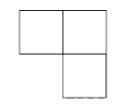
\includegraphics[width=.3in]{10-induction/L-tromino}}\ .
  %\end{center}
  Show that, for all integers $n\ge1$, a $2^n\times2^n$ sheet of graph
  paper with one corner box removed can be tiled by such trominos.
  % Found at http://math.stackexchange.com/questions/145189/examples-of-mathematical-induction
  \vfill

\end{enumerate}
\newpage


\begin{center}
  \Ovalbox{\hspace*{.25in}\parbox{5in}{{\ \hfill\Large\rule[-.2cm]{0in}{0.9cm}\textbf{Strong Mathematical Induction}\hfill \ }\\%
      %%
      Remember that the basic procedure of strong mathematical induction was
      as follows:
      \begin{enumerate}
        \item[\textbf{1.}] Prove that a statement $S_1$ is true.
        \smallskip

        \item[\textbf{2.}] Prove that, for all integers $n\ge 1$, that
          the statement $S_k$ (for $k=1,2,\ldots,n$ implies the statement $S_{n+1}$: $\{S_1,S_2,\ldots,S_n\}
          \implies S_{n+1}$.
        \smallskip

        \item[\textbf{3.}]  Conclude that $S_n$ is true for all
          integers $n\ge1$.
        \smallskip

      \end{enumerate}
      %%
    }\hspace*{0.25in}}
\end{center}
\bigskip

Prove the following using strong induction:
\begin{enumerate}
  \Problem Recall that $f_k$, the Fibonacci numbers, are defined by
  $f_1 = f_2 = 1$ and $f_{n+1} = f_n+f_{n-1}$ for $n\ge 2$.  Show that
  \begin{equation*}
    f_n = \frac{\phi^n - \psi^n}{\sqrt{5}},
  \end{equation*}
  where $\phi = \frac{1+\sqrt{5}}{2}$ is the \emph{golden ratio}\ and
  $\psi = \frac{1-\sqrt{5}}{2} = -1/\phi$.
  \vfill
\end{enumerate}

%\end{document}
\begin{comment}

\newpage
\chead{\Large\textbf{Mathematical Induction -- Answers / Solutions}}%
\lhead{}
\rhead{}
\thispagestyle{fancy}

\begin{enumerate}
  \Answer Find and prove a formula for $$\sum_{j=1}^{n}{\frac{1}{j(j+1)}}.$$
  \begin{proof}
  	We'll begin by finding a formula. Using some basic calculations, we see that the first sum is $\frac{1}{2}$ and the next is $\frac{1}{2} + \frac{1}{6} = \frac{2}{3}$, and the one after is $\frac{2}{3} + \frac{1}{12} = \frac{3}{4}$. So a natural guess would be that the sum of the first $n$ such fractions is $\frac{n}{n+1}$. 
  	
  	\textbf{Base Case:} (We covered this above but I'll write it out here for the proof) For $n=1$, we have that the sum is: $\sum_{j=1}^1 \frac{1}{j(j+1)} = \frac{1}{(1)(2)} = \frac{1}{2}$, which agrees with our formula.
  	
  	\textbf{Inductive Hypothesis:} Suppose that this formula works for some $n$, so $\sum_{j=1}^{n}{\frac{1}{j(j+1)}} = \frac{n}{n+1}$ for some specific $n$.
  	
  	\textbf{Inductive Step:} Now we need to show that the formula works for $n+1$, assuming that it works for $n$. So we want to show that the sum $$\sum_{j=1}^{n+1} \frac{1}{j(j+1)} = \frac{n+1}{n+2}.$$
  	$$\sum_{j=1}^{n+1} \frac{1}{j(j+1)} = \sum_{j=1}^n \frac{1}{j(j+1)} + \frac{1}{(n+1)(n+2)} = \frac{n}{n+1} + \frac{1}{(n+1)(n+2)} $$ $$= \frac{n(n+2) + 1}{(n+1)(n+2)} = \frac{n^2 + 2n + 1}{(n+1)(n+2)} = \frac{(n+1)^2}{(n+1)(n+2)} = \frac{n+1}{n+2} $$
  	And we're done!
  	
  \end{proof}

  \Answer The sum of the first $n$ squares of natural numbers is $\frac{n(n+1)(2n+1)}{6}$:
  \begin{equation*}
    \sum_{k=1}^{n} k^2 
    = 1 + 4 + 9 + \cdots + n^2
    = \frac{n(n+1)(2n+1)}{6}.
  \end{equation*}
  
    \begin{proof}
  	We want to proceed by induction!
  	
  	\textbf{Base Case:} For $n=1$, we have that the sum is: $\sum_{k=1}^1 k^2 = 1 = \frac{1(1+1)(2(1)+1)}{6}$, which agrees with our formula.
  	
  	\textbf{Inductive Hypothesis:} Suppose that this formula works for some $n$, so $\sum_{k=1}^n = \frac{n(n+1)(2n+1)}{6}$.
  	
  	\textbf{Inductive Step:} Now we need to show that the formula works for $n+1$, assuming that it works for $n$. So we want to show that the sum $$\sum_{k=1}^{n+1} k^2  = \frac{(n+1)(n+2)(2(n+1)+1)}{6} = \frac{(n+1)(n+2)(2n+3)}{6}.$$
  
  Here we have
  	$$\sum_{k=1}^{n+1} k^2 = \sum_{k=1}^n k^2 + (n+1)^2 =  \frac{n(n+1)(2n+1)}{6} + n^2 + 2n + 1 =  \frac{(n^2+n)(2n+1)}{6} + n^2 + 2n + 1 $$ $$= \frac{2n^3 + 3n^2 + n}{6} + n^2 + 2n + 1 = \frac{2n^3 + 9n^2 + 13n + 6}{6} = \frac{(n+1)(n+2)(2n+3)}{6} $$
  	And we're done!
  	
  \end{proof}

  \Answer 
  
  \begin{proof}
  We prove the result by induction.
  
  {\bf Base Case:} For $n=1$, we have a 2 by 2 square with one corner removed. This is exactly our tromino, and hence the base case holds.
  
  {\bf Inductive Hypothesis:} Suppose a $2^n \times 2^n$ sheet with one corner removed can be covered.
  
  {\bf Inductive Step:}  Consider a $2^{n+1}$ by $2^{n+1}$ sheet of graph paper with one corner removed. Dividing the sheet in half, we get four $2^n \times 2^n$ sheets, one of which has a corner removed. We can apply the induction hypothesis to the one with the corner removed to conclude that one can be removed by the trominos. Placing one tromino at the middle of the sheet can cover one corner from each of the remaining sheets. Now we apply the induction hypothesis to the three remaining sheets yields a covering of the entire sheet. Thus by induction, we can cover the entire sheet. Here is a picture illustrating the placement.
  
  \begin{center}
  \begin{tikzpicture}
  \draw[step=1.0,black,thin] (0,0) grid (8,8);
  \draw[line width=1mm] (4,0) -- (4,8);
  \draw[line width=1mm] (0,4) -- (8,4);
  \fill[white] (7.01,7.01)--(7.01,8.1)--(8.1,8.1)--(8.1,7.01)--(7.01,7.01);
  \fill[yellow] (3,3) -- (5,3) -- (5,4) -- (4,4) -- (4, 5) --(3,5)--(3,3);
  \end{tikzpicture}
  \end{center}
  
  \end{proof}

  \Answer Recall that $f_k$, the Fibonacci numbers, are defined by
  $f_1 = f_2 = 1$ and $f_{n+1} = f_n+f_{n-1}$ for $n\ge 2$.  Show that
  \begin{equation*}
    f_n = \frac{\phi^n - \psi^n}{\sqrt{5}},
  \end{equation*}
  where $\phi = \frac{1+\sqrt{5}}{2}$ is the \emph{golden ratio}\ and
  $\psi = \frac{1-\sqrt{5}}{2} = -1/\phi$.

  \begin{proof}
  	\textbf{Base Case:} Note that we want to prove an induction statement that depends on two cases. So we need to show that this works for $n=1$ and $2$:
  	$$f_1 = 1 = \frac{\sqrt{5}}{\sqrt{5}} =  \frac{\phi - \psi}{\sqrt{5}}$$
  	$$f_2 = 1 = \frac{4 \sqrt{5}}{4\sqrt{5}} =  \frac{ 1 + 2\sqrt{5} + 5 - (1 - 2\sqrt{5} + 5)}{4\sqrt{5}} = \frac{\phi^2 - \psi^2}{\sqrt{5}}$$
  	
  	\textbf{Inductive Hypothesis:} Suppose that this formula works for all $k$ with $1 \leq k \leq n$.
  	
  	\textbf{Inductive Step:} Now we need to show that the formula works for $n+1$, assuming that it works for all $1 \leq k \leq n$. Note that $\phi^2 = 1 + \phi$, and $\psi^2 = 1 + \psi$. We have that $f_{n+1} = f_n + f_{n-1}$ by the defn. of Fibonacci numbers, and so we can use our induction hypothesis here to substitute. Note that we needed strong induction because our usual induction hypothesis would \textbf{only} gives us $f_n$, not $f_n$ and $f_{n-1}$. Substituting in, we get:
  	$$f_{n+1} = \frac{\phi^n - \psi^n}{\sqrt{5}} + \frac{\phi^{n-1} - \psi^{n-1}}{\sqrt{5}} = \frac{\phi^{n-1} (\phi + 1) - \psi^{n-1} (\psi + 1)}{\sqrt{5}}$$
  	We can now substitute using $\psi^2 = 1 + \psi$ to get:
  	$$\frac{\phi^{n-1} (\phi^2) - \psi^{n-1} (\psi^2)}{\sqrt{5}} =  \frac{\phi^{n+1} - \psi^{n+1}}{\sqrt{5}}$$
  	which proves our formula.
  \end{proof}

\end{enumerate}

\end{comment}
%\end{document}


%%% Local Variables: 
%%% mode: latex
%%% TeX-master: t
%%% End: 

\null\pagebreak 

\setcounter{problemnumber}{0}%
\setcounter{defn}{0}%
\include{11-linear-transformations/11-linear-transformations_nohead}
\null\pagebreak 

\setcounter{problemnumber}{0}%
\setcounter{defn}{0}%
\include{12-linear-transformations-matrix/12-linear-transformations-mat_nohead}
\null\pagebreak 

\setcounter{problemnumber}{0}%
\setcounter{defn}{0}%
%\documentclass[12pt,letterpaper]{article}



%%%
%% Required packages:
%%
\usepackage{etex}
\usepackage{amsmath}
\usepackage{amssymb}
\usepackage{amstext}
\usepackage{amsthm}
\usepackage{fancyhdr,fancybox}
\usepackage{mathrsfs} % need for \mathscr command
\usepackage{multicol}
\usepackage[normalem]{ulem}
%\usepackage{pictex,pictexplus}
% \usepackage{pictexwd}
\usepackage{rotating}
\usepackage{url}
\usepackage{xfrac}
\usepackage{booktabs}
\usepackage{color,soul}
\usepackage{comment}

\usepackage{hyperref}
\hypersetup{
    colorlinks=true,     % false: boxed links; true: colored links
    linkcolor=blue,      % color of internal links
    citecolor=blue,      % color of links to bibliography
    filecolor=blue,      % color of file links
    urlcolor=blue        % color of external links
}


\usepackage{tikz}
\usetikzlibrary{backgrounds,calc}

%%
%% Common formatting commands
%%
\setlength{\parindent}{0in}
\setlength{\textwidth}{7in}
\setlength{\evensidemargin}{-0.25in}
\setlength{\oddsidemargin}{-0.25in}
\setlength{\parskip}{.5\baselineskip}
\setlength{\topmargin}{-0.5in}
\setlength{\textheight}{9in}

%               Problem and Part
\newcounter{problemnumber}
\newcounter{partnumber}
\newcounter{subpartnumber}
\newcommand{\Problem}{%
  \refstepcounter{problemnumber}%
  \setcounter{partnumber}{0}%
  \setcounter{subpartnumber}{0}%
  \item[\makebox{\hfil\textbf{\theproblemnumber.}\hfil}]%
  }
\newcommand{\InProblem}[2][1.6]{%
  \refstepcounter{problemnumber}%
  \setcounter{partnumber}{0}%
  \setcounter{subpartnumber}{0}%
  \textbf{\theproblemnumber.}\ \ \parbox[t]{#1in}{#2}%
}
\newcommand{\InSmallProblem}[1]{\InProblem[1.05]{#1}}
\newcommand{\NoProblem}[1]{%
  \mbox{\hfil\textbf{#1}\hfil}%
  }
\newcommand{\UnProblem}{%
  \refstepcounter{problemnumber}%
  \setcounter{partnumber}{0}%
  \setcounter{subpartnumber}{0}%
  \mbox{\hfil\textbf{\theproblemnumber.}\hfil}%
  }
\newcommand{\InFlexProblem}[1]{%
  \refstepcounter{problemnumber}%
  \setcounter{partnumber}{0}%
  \setcounter{subpartnumber}{0}%
  \textbf{\theproblemnumber.}\ \ #1%
}
%%  Part:
\newcommand{\Part}{%
  \renewcommand{\thepartnumber}{(\alph{partnumber})}%
  \refstepcounter{partnumber}
  \setcounter{subpartnumber}{0}%
  \item[(\alph{partnumber})]%
}
\newcommand{\InPart}[2][1.75]{%
  \renewcommand{\thepartnumber}{(\alph{partnumber})}%
  \refstepcounter{partnumber}%
  \setcounter{subpartnumber}{0}%
  (\alph{partnumber})\ \ \parbox[t]{#1in}{#2}%
}
\newcommand{\UnPart}{%
  \refstepcounter{partnumber}%
  \renewcommand{\thepartnumber}{(\alph{partnumber})}%
  \setcounter{subpartnumber}{0}%
  (\alph{partnumber})%
}
\newcommand{\InLargePart}[1]{\InPart[3.05]{#1}}
\newcommand{\InFullPart}[1]{\InPart[6.2]{#1}}
\newcommand{\InSmallPart}[1]{\InPart[1.05]{#1}}
%% SubPart:
\newcommand{\SubPart}{%
  \refstepcounter{subpartnumber}%
  \item[(\roman{subpartnumber})]%
  }
\newcommand{\InSubPart}[2][2.25]{%
  \stepcounter{subpartnumber}%
  (\roman{subpartnumber})\ \ \parbox[t]{#1in}{#2}%
}
\newcommand{\InSmallSubPart}[1]{\InSubPart[1.5]{#1}}
\newcommand{\InTinySubPart}[1]{%
  \stepcounter{subpartnumber}%
  (\roman{subpartnumber})\ \ \makebox{#1}%
}
\newcommand{\InMySubPart}[2][2.25]{%
  \stepcounter{subpartnumber}%
  \parbox[t]{#1in}{\makebox[0.3in][l]{(\roman{subpartnumber})}\ \ {#2}}%
}
\newcommand{\TrueFalse}{\textbf{T}\ \ \textbf{F}\ \ }
\newcommand{\TFPart}[1]{% 
  \stepcounter{partnumber}%
  \setcounter{subpartnumber}{0}%
  \item[(\alph{partnumber})] \TrueFalse\parbox[t]{5.5in}{#1}}

\newcommand{\Points}[1]{(#1 points) \ }
\newcommand{\Point}[1]{(#1 point) \ }


%% For Answers:
\newcounter{answernumber}
\newcommand{\Answer}{%
  \refstepcounter{answernumber}%
  \setcounter{partnumber}{0}%
  \setcounter{subpartnumber}{0}%
  \item[\makebox{\hfil\textbf{\theanswernumber.}\hfil}]%
  }


% Setting up the headers for the first page
%\chead{} % will default to what is typed in the file.
\fancyhead[L]{\textsc{Math 22a}}
\fancyhead[R]{\textsc{Fall 2024}}
\fancyfoot[R]{
	\vspace*{\fill}\footnotesize\textcopyright{} \emph{Harvard Math 22a}	
}
\renewcommand{\headrulewidth}{0pt}

%\fancyhead[C]{}
%	\chead{}	
%	\lhead{}
%	\rhead{}
%	\cfoot{}


% Putting copyright on the footer of each page
%\fancypagestyle{secondpage}{
%	\fancyhead[C]{TESTing again} % change this to be blank
%		%\chead{}	
%	\fancyhead[L]{bears} % change this to be blank
%	\fancyhead[R]{dogs} % change this to be blank
%	\fancyfoot[R]{ %keeps the footer the same
%		\vspace*{\fill}\footnotesize\textcopyright{} \emph{Harvard Math 22a}	
%	}
%}
%\renewcommand{\headrulewidth}{0pt}
%\pagestyle{fancy}
\pagestyle{empty}


%\lhead{}
%\rhead{}
%\rfoot{\vspace*{\fill}\footnotesize\textcopyright{} \emph{Harvard Math 22a}}
%\renewcommand{\headrulewidth}{0pt}
%\pagestyle{fancy}




%%
%% Common shortcut commands:
%%
\newcommand{\ds}{\displaystyle}
\newcommand{\sgn}{\operatorname{sgn}}
\renewcommand{\Pr}{\operatorname{P}}
\newcommand{\CPr}[3][{}]{\Pr_{\text{#1}}\left(#2\,|\,#3\right)}

\newcommand{\C}{\mathbb{C}}
\newcommand{\R}{\mathbb{R}}
\newcommand{\Z}{\mathbb{Z}}
\newcommand{\N}{\mathbb{N}}
\newcommand{\Q}{\mathbb{Q}}
\newcommand{\D}{\mathbb{D}}

\newcommand{\rref}{\operatorname{rref}}
\newcommand{\im}{\operatorname{im}}
\newcommand{\rank}{\operatorname{rank}}
\newcommand{\diag}{\operatorname{diag}}
\newcommand{\Span}{\operatorname{span}}
%\renewcommand{\vec}[1]{\mathbf{#1}}
\newcommand{\charpoly}{\mathscr{P}}
\newcommand{\nicefrac}[2]{\sfrac{#1}{#2}} % using xfrac package
\newcommand{\topology}{\mathcal{T}}
\newcommand{\Inn}{\operatorname{Inn}}

\newcommand{\blankbox}[2]{\fbox{\rule{#1}{0in}\rule{0in}{#2}}}

\newenvironment{myindentpar}[1]%
 {\begin{list}{}%
         {\setlength{\leftmargin}{#1}
          \setlength{\rightmargin}{\leftmargin}}%
         \item[]%
 }
 {\end{list}}
\newtheorem{theorem}{Theorem}
\newtheorem*{NStheorem}{Theorem}
\newtheorem{cor}[theorem]{Corollary}
\newtheorem*{claim}{Claim}
\newtheorem{defn}{Definition}

\newenvironment{amatrix}[1]{%
  \left(\begin{array}{@{}*{#1}{c}|c@{}}
}{%
  \end{array}\right)
}

%--------grstep
% For denoting a Gauss' reduction step.
% Use as: \grstep{\rho_1+\rho_3} or \grstep[2\rho_5 \\ 3\rho_6]{\rho_1+\rho_3}
\newcommand{\grstep}[2][\relax]{%
   \ensuremath{\mathrel{
       {\mathop{\longrightarrow}\limits^{#2\mathstrut}_{
                                     \begin{subarray}{l} #1 \end{subarray}}}}}}
\newcommand{\swap}{\leftrightarrow}




\section{{Matrix Operations, $\vec{\S}$2.1, 2.2}}% 
\chead{\Large\textbf{Matrix Operations, $\vec{\S}$2.1, 2.2}}% 

%\begin{document}
\thispagestyle{fancy}

Recall from last class:

\begin{itemize}

\item {\bf Theorem 10:} Let $T: \R^n \to \R^m$ be linear. Then there exists a unique matrix $A$ such that $T(\vec{x})=A\vec{x}$ for all $\vec{x} \in \R^n$; namely $A=[T(\vec{e}_1) \; \dots \; T(\vec{e}_n)]$.
\item {\bf Theorem 11:} Let $T: \R^n \to \R^m$ be linear. Then $T$ is injective if and only if $T(\vec{x})=\vec{0}$ has only the trivial solution.
\item {\bf Theorem 12:} Let $T: \R^n \to \R^m$ be linear, and let $A$ be the associated matrix. Then 
\begin{enumerate}
\item $T$ is surjective if and only if the columns of $A$ span $\R^m$.
\item $T$ is injective if and only if the columns of $A$ are linearly independent. 
\end{enumerate}
\end{itemize}

\newpage

Let $A=[\vec{a}_1 \; \dots \; \vec{a}_n]$ be an $m$ by $n$ matrix. We express $A$ by
$$A=\begin{bmatrix}
a_{11} & a_{12} & \hdots & a_{1n}\\ 
a_{21} & a_{22} & \hdots & a_{2n}\\ 
\vdots & & \ddots & \vdots\\
a_{n1} & a_{n2} & \hdots & a_{nn}\\ 
\end{bmatrix}$$
where $a_{ij}$ is the entry in the $i$-th row and $j$-th column.

{\bf Theorem:} Let $A$, $B$, and $C$ be matrices of the same size, and let $r$ and $s$ be real numbers. Then the following properties hold:
\begin{enumerate}
\item $A+B=B+A$.
\item $(A+B)+C=A+(B+C)$.
\item $A+0=A$.
\item $r(A+B)=rA+rB$.
\item $(r+s)A=rA+sA$.
\item $r(sA)=rsA$.
\end{enumerate}

\begin{defn}
If $A$ is a $m\times n$ matrix and $B$ is an $n\times p$ matrix with columns $\vec{b}_1, \dots, \vec{b}_p$, then $AB$ is the $m \times p$ matrix given by $$AB=A[\vec{b}_1 \; \dots \; \vec{b}_p]=[A\vec{b}_1 \; \dots \; A\vec{b}_p].$$
\end{defn}

\begin{enumerate}

\Problem Compute $AB$ when $$A=\begin{bmatrix} 2 & 3\\ 1 & -5\\ \end{bmatrix} \text{ and } B=\begin{bmatrix} 4 & 3 & 6\\ 1 & -2 & 3\\ \end{bmatrix}.$$ Can you also compute $BA$?

\newpage


{\bf Remark:}
$$(AB)_{ij}=a_{i1}b_{1j}+a_{i2}b_{2j}+\dots+a_{in}b_{nj}.$$

{\bf Properties of Matrix Multiplication.}

{\bf Theorem:}
\begin{enumerate}
\item $A(BC)=(AB)C$.
\item $A(B+C)=AB+AC$.
\item $(B+C)A=BA+CA$.
\item $r(AB)=(rA)B=A(rB)$.
\item $I_m A =A = AI_n$.
\end{enumerate}

\Problem {\bf True or False Questions.} Prove or give a counterexample as appropriate. Suppose $A$ and $B$ are $n$ by $n$ matrices.

\begin{enumerate}
\item $AB=BA$.

\vfill

\item If $AB=0$, then $A=0$ or $B=0$.

\vfill

\item If $A^2=0$, then $A=0$.

\vfill

\item If $AB=AC$, then $B=C$.

\vfill

\end{enumerate}

\newpage


\begin{defn}
Given an $m\times n$ matrix $A$, then the {\bf transpose of $A$}, denoted $A^{T}$ is the $n \times m$ matrix given by taking the columns of $A$ as rows.
\end{defn}

{\bf Theorem:} Let $A$ be an $m$ by $n$ matrix, $B$ be an $n$ by $p$ matrix, and $r\in \R$.
\begin{enumerate}
\item $(A^{T})^{T}=A.$
\item $(A+B)^{T}=A^{T}+B^{T}.$
\item $(rA)^{T}=r A^{T}$.
\item $(AB)^{T}=B^{T} A^{T}$.
\end{enumerate}

\begin{defn}
An $n$ by $n$ matrix $A$ is {\bf invertible} if there is an $n$ by $n$ matrix $C$ so that $AC=I$ and $CA=I$. We denote the inverse of $A$ by $A^{-1}$.
\end{defn}

{\bf Natural Questions:}
\begin{enumerate}
\item Do inverses always exist?
\item If not, when do they exist?
\item If they exist, are they unique?
\item How can we find them?
\end{enumerate}

\Problem Let $A=\begin{bmatrix} a & b\\ c & d\\ \end{bmatrix}$. Determine when $A$ is invertible and find $A^{-1}$. 

\newpage

{\bf Theorem:} Let $A=\begin{bmatrix} a & b \\ c & d\\ \end{bmatrix}$. If $ad-bc\neq 0$, then $A$ is invertible  and $$A^{-1}= \frac{1}{ad-bc} \begin{bmatrix} d & -b\\ -c &a \\ \end{bmatrix}.$$

\begin{defn}
We define the {\bf determinant} of $A=\begin{bmatrix} a & b \\ c & d\\ \end{bmatrix}$, denoted by $\text{det}(A)$, by $$\text{det}(A)=ad-bc.$$
\end{defn}

{\bf Theorem:} If $A$ is an $n$ by $n$ invertible matrix, then for each $\vec{b}\in \R^n$, $A\vec{x}=\vec{b}$ has a unique solution; namely $\vec{x}=A^{-1}\vec{b}$.

\Problem Prove the Theorem.

\vfill

\newpage

{\bf Theorem:} Suppose $A$ and $B$ are $n$ by $n$ matrices, then the following hold. 
\begin{enumerate}
\item If $A$ is invertible, then $A^{-1}$ is invertible and $(A^{-1})^{-1}=A$.
\item $(AB)^{-1}=B^{-1} A^{-1}$.
\item $(A^{T})^{-1}=(A^{-1})^{T}$.
\end{enumerate}

\Problem Prove the Theorem.

 

\end{enumerate}

\begin{comment}

\newpage
\chead{\Large\textbf{Matrix Operations -- Answers / Solutions}}%
\lhead{}
\rhead{}
\thispagestyle{fancy}

\begin{enumerate}
\Answer Let $$A=\begin{bmatrix} 2 & 3\\ 1 & -5\\ \end{bmatrix} \text{ and } B=\begin{bmatrix} 4 & 3 & 6\\ 1 & -2 & 3\\ \end{bmatrix},$$ then using the definition of matrix multiplication we get the following
$$A\vec{b}_1 =\begin{bmatrix}
2(4)+3(1)\\
1(4)-5(1)\\
\end{bmatrix}=\begin{bmatrix}
11\\
-1\\
\end{bmatrix}, A\vec{b}_2 =\begin{bmatrix}
2(3)+3(-2)\\
1(3)-5(-2)\\
\end{bmatrix}=\begin{bmatrix}
0\\
13\\
\end{bmatrix}, \text{ and } A\vec{b}_3 =\begin{bmatrix}
2(6)+3(3)\\
1(6)-5(3)\\
\end{bmatrix}=\begin{bmatrix}
21\\
-9\\
\end{bmatrix}.$$

Hence $$AB=[A\vec{b_1} \; A\vec{b}_2 \; A\vec{b}_3]=\begin{bmatrix}
11 & 0 & 21\\
-1 & 13 & -9\\
\end{bmatrix}.$$

We cannot multiply the matrices in the other order as the number of rows of $A$ does not equal the number of columns of $B$, and hence $BA$. In terms of the corresponding linear transformations, this says the number of outputs of $A$ does not match the number of inputs of $B$, and hence we cannot compose the functions in that order.
  
\Answer   

\begin{enumerate}

\item {\bf False.} There are many counterexamples, but take for instance $A=\begin{bmatrix} 1 & 2\\ 3 & 4\\ \end{bmatrix}$, and $B=\begin{bmatrix} 0 & 1\\ -1 & 1\\ \end{bmatrix}$, then $AB=\begin{bmatrix} -2 & 3\\ -4 & 7\\ \end{bmatrix}$ and $BA=\begin{bmatrix} 3 & 4\\ 2 & 2\\ \end{bmatrix}$. Thus $AB\neq BA$.

\item {\bf False.} Let $A=\begin{bmatrix} 1 & 1\\ 2 & 2\\ \end{bmatrix}$, and $B=\begin{bmatrix} 1 & 1\\ -1 & -1\\ \end{bmatrix}$, then $AB=\begin{bmatrix} 0 & 0\\ 0 & 0\\ \end{bmatrix}$.

\item {\bf False.} Let $A=\begin{bmatrix} 0 & 1\\ 0 & 0\\ \end{bmatrix}$, then $A^2=\begin{bmatrix} 0 & 0\\ 0 & 0\\ \end{bmatrix}$.

\item {\bf False.} Let $$A=\begin{bmatrix} 0 & 1\\ 0 & 1\\ \end{bmatrix}, B=\begin{bmatrix} 1 & 1\\ 0 & 1\\ \end{bmatrix}\text{, and  } C=\begin{bmatrix} 2 & 1\\ 0 & 1\\ \end{bmatrix},$$  then $AB=AC$ but $B\neq C$.

\end{enumerate}
    
\Answer We want to find $e$, $f$, $g$ and $h$ such that 
$$\begin{bmatrix}
a & b\\
c & d\\
\end{bmatrix}\begin{bmatrix}
e & f\\
g &h\\
\end{bmatrix}=\begin{bmatrix}
1 & 0\\
0 & 1\\
\end{bmatrix}.$$
Thus we get the following system of equations:
\begin{align*}
ae+gb&=1\\
af+bh&=0\\
ce+dg&=0\\
cf+dh&=1\\
\end{align*}

Multplying the first equation by $c$ and the third equation by $-a$ and adding them together yields: $bcg-adg=c$, and assuming $ad-bc\neq0$, we get $g=\frac{-c}{ad-bc}$.

Continuing in a similar manner we get $e=\frac{d}{ad-bc}$, $h=\frac{a}{ad-bc}$, and $f=\frac{-b}{ad-bc}$.

Thus the matrix is invertible if and only if $ad-bc\neq0$, and we have an explicit formula for the inverse matrix.
  
\Answer Since $A$ is invertible, we know $A^{-1}$ exists. Let $\vec{x}=A^{-1}\vec{b}$, then we check $\vec{x}$ is a solution. Here $A\vec{x}=AA^{-1}\vec{b}=\vec{b}$, and hence $\vec{x}$ is a solution.

Now we check it is the unique solution. Suppose $\vec{u}$ is another solution, then $A\vec{u}=\vec{b}$. Since $A$ is invertible, we can multiply both sides by $A^{-1}$ to get $A^{-1}A\vec{u}=A^{-1}\vec{b}$, and hence $\vec{u}=A^{-1}\vec{b}=\vec{x}$. Thus $\vec{x}$ is the only solution.
  
\Answer 

\begin{enumerate}
	
\Part Suppose $A$ is invertible. We check that $A$ is the inverse of $A^{-1}$; namely, $AA^{-1}=I_n$ and $A^{-1}A=I_n$. Thus the inverse of $A^{-1}$ is $A$; in symbols $(A^{-1})^{-1}=A$.

\Part Again suppose $A$ and $B$ are both invertible matrices. We check that $B^{-1}A^{-1}$ is the inverse of $AB$: $ABB^{-1}A^{-1}=I_n$ and $B^{-1}A^{-1}AB=I_n$. Thus by the definition of inverse matrix, $B^{-1}A^{-1}$ is the inverse of $AB$; i.e. $(AB)^{-1}=B^{-1}A^{-1}$.

\Part Suppose $A$ is an invertible matrix. We want to prove that the inverse of $A^{T}$ is $(A^{-1})^{T}$. Again we check the conditions in the definition of matrix inverse: $A^{T}(A^{-1})^{T}=(A^{-1}A)^{T}=(I_n)^{T}=I_n$ and $(A^{-1})^{T}A^{T}=(AA^{-1})^{T}=(I_n)^{T}=I_n$ where we used $(AB)^{T}=B^{T}A^{T}$. Thus $(A^{T})^{-1}=(A^{-1})^{T}$.

\end{enumerate}
\end{enumerate}

\end{comment}
%\end{document}



%%% Local ables: 
%%% mode: latex
%%% TeX-master: t
%%% End: 

\null\pagebreak 

\setcounter{problemnumber}{0}%
\setcounter{defn}{0}%
\include{14-inverses/14-inverses_nohead}
\null\pagebreak 

\setcounter{problemnumber}{0}%
\setcounter{defn}{0}%
%\documentclass[12pt,letterpaper]{article}



%%%
%% Required packages:
%%
\usepackage{etex}
\usepackage{amsmath}
\usepackage{amssymb}
\usepackage{amstext}
\usepackage{amsthm}
\usepackage{fancyhdr,fancybox}
\usepackage{mathrsfs} % need for \mathscr command
\usepackage{multicol}
\usepackage[normalem]{ulem}
%\usepackage{pictex,pictexplus}
% \usepackage{pictexwd}
\usepackage{rotating}
\usepackage{url}
\usepackage{xfrac}
\usepackage{booktabs}
\usepackage{color,soul}
\usepackage{comment}

\usepackage{hyperref}
\hypersetup{
    colorlinks=true,     % false: boxed links; true: colored links
    linkcolor=blue,      % color of internal links
    citecolor=blue,      % color of links to bibliography
    filecolor=blue,      % color of file links
    urlcolor=blue        % color of external links
}


\usepackage{tikz}
\usetikzlibrary{backgrounds,calc}

%%
%% Common formatting commands
%%
\setlength{\parindent}{0in}
\setlength{\textwidth}{7in}
\setlength{\evensidemargin}{-0.25in}
\setlength{\oddsidemargin}{-0.25in}
\setlength{\parskip}{.5\baselineskip}
\setlength{\topmargin}{-0.5in}
\setlength{\textheight}{9in}

%               Problem and Part
\newcounter{problemnumber}
\newcounter{partnumber}
\newcounter{subpartnumber}
\newcommand{\Problem}{%
  \refstepcounter{problemnumber}%
  \setcounter{partnumber}{0}%
  \setcounter{subpartnumber}{0}%
  \item[\makebox{\hfil\textbf{\theproblemnumber.}\hfil}]%
  }
\newcommand{\InProblem}[2][1.6]{%
  \refstepcounter{problemnumber}%
  \setcounter{partnumber}{0}%
  \setcounter{subpartnumber}{0}%
  \textbf{\theproblemnumber.}\ \ \parbox[t]{#1in}{#2}%
}
\newcommand{\InSmallProblem}[1]{\InProblem[1.05]{#1}}
\newcommand{\NoProblem}[1]{%
  \mbox{\hfil\textbf{#1}\hfil}%
  }
\newcommand{\UnProblem}{%
  \refstepcounter{problemnumber}%
  \setcounter{partnumber}{0}%
  \setcounter{subpartnumber}{0}%
  \mbox{\hfil\textbf{\theproblemnumber.}\hfil}%
  }
\newcommand{\InFlexProblem}[1]{%
  \refstepcounter{problemnumber}%
  \setcounter{partnumber}{0}%
  \setcounter{subpartnumber}{0}%
  \textbf{\theproblemnumber.}\ \ #1%
}
%%  Part:
\newcommand{\Part}{%
  \renewcommand{\thepartnumber}{(\alph{partnumber})}%
  \refstepcounter{partnumber}
  \setcounter{subpartnumber}{0}%
  \item[(\alph{partnumber})]%
}
\newcommand{\InPart}[2][1.75]{%
  \renewcommand{\thepartnumber}{(\alph{partnumber})}%
  \refstepcounter{partnumber}%
  \setcounter{subpartnumber}{0}%
  (\alph{partnumber})\ \ \parbox[t]{#1in}{#2}%
}
\newcommand{\UnPart}{%
  \refstepcounter{partnumber}%
  \renewcommand{\thepartnumber}{(\alph{partnumber})}%
  \setcounter{subpartnumber}{0}%
  (\alph{partnumber})%
}
\newcommand{\InLargePart}[1]{\InPart[3.05]{#1}}
\newcommand{\InFullPart}[1]{\InPart[6.2]{#1}}
\newcommand{\InSmallPart}[1]{\InPart[1.05]{#1}}
%% SubPart:
\newcommand{\SubPart}{%
  \refstepcounter{subpartnumber}%
  \item[(\roman{subpartnumber})]%
  }
\newcommand{\InSubPart}[2][2.25]{%
  \stepcounter{subpartnumber}%
  (\roman{subpartnumber})\ \ \parbox[t]{#1in}{#2}%
}
\newcommand{\InSmallSubPart}[1]{\InSubPart[1.5]{#1}}
\newcommand{\InTinySubPart}[1]{%
  \stepcounter{subpartnumber}%
  (\roman{subpartnumber})\ \ \makebox{#1}%
}
\newcommand{\InMySubPart}[2][2.25]{%
  \stepcounter{subpartnumber}%
  \parbox[t]{#1in}{\makebox[0.3in][l]{(\roman{subpartnumber})}\ \ {#2}}%
}
\newcommand{\TrueFalse}{\textbf{T}\ \ \textbf{F}\ \ }
\newcommand{\TFPart}[1]{% 
  \stepcounter{partnumber}%
  \setcounter{subpartnumber}{0}%
  \item[(\alph{partnumber})] \TrueFalse\parbox[t]{5.5in}{#1}}

\newcommand{\Points}[1]{(#1 points) \ }
\newcommand{\Point}[1]{(#1 point) \ }


%% For Answers:
\newcounter{answernumber}
\newcommand{\Answer}{%
  \refstepcounter{answernumber}%
  \setcounter{partnumber}{0}%
  \setcounter{subpartnumber}{0}%
  \item[\makebox{\hfil\textbf{\theanswernumber.}\hfil}]%
  }


% Setting up the headers for the first page
%\chead{} % will default to what is typed in the file.
\fancyhead[L]{\textsc{Math 22a}}
\fancyhead[R]{\textsc{Fall 2024}}
\fancyfoot[R]{
	\vspace*{\fill}\footnotesize\textcopyright{} \emph{Harvard Math 22a}	
}
\renewcommand{\headrulewidth}{0pt}

%\fancyhead[C]{}
%	\chead{}	
%	\lhead{}
%	\rhead{}
%	\cfoot{}


% Putting copyright on the footer of each page
%\fancypagestyle{secondpage}{
%	\fancyhead[C]{TESTing again} % change this to be blank
%		%\chead{}	
%	\fancyhead[L]{bears} % change this to be blank
%	\fancyhead[R]{dogs} % change this to be blank
%	\fancyfoot[R]{ %keeps the footer the same
%		\vspace*{\fill}\footnotesize\textcopyright{} \emph{Harvard Math 22a}	
%	}
%}
%\renewcommand{\headrulewidth}{0pt}
%\pagestyle{fancy}
\pagestyle{empty}


%\lhead{}
%\rhead{}
%\rfoot{\vspace*{\fill}\footnotesize\textcopyright{} \emph{Harvard Math 22a}}
%\renewcommand{\headrulewidth}{0pt}
%\pagestyle{fancy}




%%
%% Common shortcut commands:
%%
\newcommand{\ds}{\displaystyle}
\newcommand{\sgn}{\operatorname{sgn}}
\renewcommand{\Pr}{\operatorname{P}}
\newcommand{\CPr}[3][{}]{\Pr_{\text{#1}}\left(#2\,|\,#3\right)}

\newcommand{\C}{\mathbb{C}}
\newcommand{\R}{\mathbb{R}}
\newcommand{\Z}{\mathbb{Z}}
\newcommand{\N}{\mathbb{N}}
\newcommand{\Q}{\mathbb{Q}}
\newcommand{\D}{\mathbb{D}}

\newcommand{\rref}{\operatorname{rref}}
\newcommand{\im}{\operatorname{im}}
\newcommand{\rank}{\operatorname{rank}}
\newcommand{\diag}{\operatorname{diag}}
\newcommand{\Span}{\operatorname{span}}
%\renewcommand{\vec}[1]{\mathbf{#1}}
\newcommand{\charpoly}{\mathscr{P}}
\newcommand{\nicefrac}[2]{\sfrac{#1}{#2}} % using xfrac package
\newcommand{\topology}{\mathcal{T}}
\newcommand{\Inn}{\operatorname{Inn}}

\newcommand{\blankbox}[2]{\fbox{\rule{#1}{0in}\rule{0in}{#2}}}

\newenvironment{myindentpar}[1]%
 {\begin{list}{}%
         {\setlength{\leftmargin}{#1}
          \setlength{\rightmargin}{\leftmargin}}%
         \item[]%
 }
 {\end{list}}
\newtheorem{theorem}{Theorem}
\newtheorem*{NStheorem}{Theorem}
\newtheorem{cor}[theorem]{Corollary}
\newtheorem*{claim}{Claim}
\newtheorem{defn}{Definition}

\newenvironment{amatrix}[1]{%
  \left(\begin{array}{@{}*{#1}{c}|c@{}}
}{%
  \end{array}\right)
}

%--------grstep
% For denoting a Gauss' reduction step.
% Use as: \grstep{\rho_1+\rho_3} or \grstep[2\rho_5 \\ 3\rho_6]{\rho_1+\rho_3}
\newcommand{\grstep}[2][\relax]{%
   \ensuremath{\mathrel{
       {\mathop{\longrightarrow}\limits^{#2\mathstrut}_{
                                     \begin{subarray}{l} #1 \end{subarray}}}}}}
\newcommand{\swap}{\leftrightarrow}



%\makeatletter
%\renewcommand*\env@matrix[1][*\c@MaxMatrixCols c]{%
%	\hskip -\arraycolsep
%	\let\@ifnextchar\new@ifnextchar
%	\array{#1}}
%\makeatother
%
%\def\env@matrix{\hskip -\arraycolsep
%	\let\@ifnextchar\new@ifnextchar
%	\array{*\c@MaxMatrixCols c}}
%

\section{{Determinants, $\vec\S$2.3}}% 
\chead{\Large\textbf{Determinants, $\vec\S$2.3}}% 

%\begin{document}
\thispagestyle{fancy}

Recall from the last few classes:

\begin{itemize}
\item We define the {\bf determinant} of $A=\begin{bmatrix} a & b \\ c & d\\ \end{bmatrix}$, denoted by $\text{det}(A)$, by $$\text{det}(A)=ad-bc.$$
\item {\bf Theorem:} If $A$ is an $n$ by $n$ invertible matrix, then for each $\vec{b}\in \R^n$, $A\vec{x}=\vec{b}$ has a unique solution; namely $\vec{x}=A^{-1}\vec{b}$.
\item {\bf Theorem:} Suppose $A$ and $B$ are $n$ by $n$ invertible matrices, then the following hold. 
\begin{enumerate}
\item $A^{-1}$ is invertible and $(A^{-1})^{-1}=A$.
\item $(AB)^{-1}=B^{-1} A^{-1}$.
\item $(A^{T})^{-1}=(A^{-1})^{T}$.
\end{enumerate}
\item An {\bf elementary matrix} $E$ is a matrix obtained from the identity matrix by a single elementary row operation.
 \item {\bf Theorem:} $A$ is invertible if and only if $A$ is row equivalent to the identity matrix. Furthermore, any sequence of elementary row operations that reduces $A$ to $I_n$ also transforms $I_n$ into $A^{-1}$.
\end{itemize}

\newpage





\begin{enumerate}

\Problem 
\Part Let $A=\begin{bmatrix}
1 & -2 & -1\\
-1 &5 & 6\\
5 &-4 & 5\\
\end{bmatrix}$. Find $A^{-1}$ if possible.

\vfill

\Part Let $A=\begin{bmatrix}
1 & 0 & -2\\
-3 &1 & 4\\
2 &-3 & 4\\
\end{bmatrix}$. Find $A^{-1}$ if possible.

\vfill

\newpage

{\bf Invertible Matrix Theorem} Let $A$ be an $n \times n$ matrix, then the following are all equivalent.
\begin{enumerate}
\item $A$ is invertible.
\item $A$ is row-equivalent to $I_n$.
\item $A$ has $n$ pivot positions.
\item $A\vec{x}=\vec{0}$ has only the trivial solution.
\item The columns of $A$ are linearly independent.
\item $x\mapsto A\vec{x}$ is one-to-one (injective).
\item For all $\vec{b}\in \R^n$, $A\vec{x}=\vec{b}$ is consistent.
\item The columns of $A$ span $\R^n$.
\item $\vec{x} \mapsto A\vec{x}$ is onto (surjective).
\item There exists a matrix $C$ such that $CA=I_n$.
\item There exists a matrix $D$ such that $AD=I_n$.
\item $A^{T}$ is invertible.
\end{enumerate}

\Problem Prove the theorem.

\newpage

\Problem Determine if the following matrices are invertible.
\Part Let $A=\begin{bmatrix}
3 & 0 & 0\\
-3 &-4 & 0\\
8 & 5 & -3\\
\end{bmatrix}$.

\vfill

\Part Let $A=\begin{bmatrix}
1 &2 & 3\\
4 &5 & 6\\
7 & 8 & 9\\
\end{bmatrix}$.

\vfill

\newpage

{\bf Theorem:} Let $T: \R^n \to \R^n$ be linear and let $A$ be the associated matrix. Then $T$ is invertible if and only if $A$ is invertible.

\Problem Prove the theorem.

\newpage

{\bf Goal:} Develop a numerical test for invertibility.

\Problem Let $A=\begin{bmatrix}
a & b & c\\
d & e &f\\
g & h & i\\
\end{bmatrix}$. Find a condition on the entries of $A$ for $A$ to be invertible.

\newpage

\begin{defn}
For a matrix $A$ define  $A_{ij}$ to be the matrix obtained from $A$ by deleting row $i$ and column $j$.
\end{defn}

{\bf Remark:} $$\text{det} \begin{bmatrix}
a & b & c\\
d & e &f\\
g & h & i\\
\end{bmatrix} = a \text{det} A_{11} - b \text{det} A_{12} +c \text{det} A_{13}.$$

\begin{defn}
For $n\geq 2$, the determinant of an $n\times n$ matrix $A=[a_{ij}]$ is
\begin{equation*}
\operatorname{det}(A)= a_{11} \operatorname{det}(A_{11}) - a_{12} \operatorname{det}(A_{12})+\dots + (-1)^{n+1} a_{1n} \operatorname{det}(A_{1n})=\sum_{j=1}^{n}(-1)^{1+j}a_{1j} \operatorname{det}(A_{1j}).
\end{equation*}
\end{defn}

\Problem Compute the determinant of $A=\begin{bmatrix}
1 & 2 &3\\
4 & 5 &6\\
7 & 8 & 9\\
\end{bmatrix}$.

\vfill

\begin{defn} The {\bf $(i,j)$-cofactor} of $A$ is given by $c_{ij} =(-1)^{i+j} \operatorname{det} A_{ij}$, and the {\bf cofactor expansion along row $i$} is given by $\sum_{j=1}^{n}a_{ij} c_{ij}$.
\end{defn}



{\bf Theorem 3.1:} Cofactor expansion across any row or column is the same, and hence each cofactor expansion gives the determinant.

\newpage

\Problem Compute the determinant of 
$C=\begin{bmatrix}
6 & 0 & 0 & 5\\
1 & 7 & 2 & -5\\
2 & 0 & 0 & 0\\
8 & 3 & 1 & 8\\
\end{bmatrix}$.

\vfill

\begin{defn} Let $A=[a_{ij}]$ be an $n\times n$ matrix, then $A$ is {\bf upper triangular} if $a_{ij}=0$ when $i>j$.
\end{defn}

{\bf Theorem 3.2:} Let $A$ be an $n\times n$ upper triangular matrix, then $$\operatorname{det}(A)= a_{11}a_{22}\dots a_{nn} = \prod_{j=1}^n a_{jj}.$$

\Problem Prove the theorem.

\vfill
\vfill

\end{enumerate}

\begin{comment}
%\end{document}

\newpage
\chead{\Large\textbf{Determinants -- Answers / Solutions}}%
\lhead{}
\rhead{}
\thispagestyle{fancy}

\begin{enumerate}
  \Answer
  
 \begin{enumerate} 
  \Part Let $A=\begin{bmatrix}
  1 & -2 & -1\\
  -1 &5 & 6\\
  5 &-4 & 5\\
  \end{bmatrix}$. We try augment $A$ by $I_n$ and try to use the result that if $A$ is invertible, then $[A|I_n]\sim [I_n | A^{-1}]$. Thus
  
  \begin{align*}
  \begin{pmatrix}[ccc|ccc]
  1 & -2 & -1 & 1 & 0 & 0\\
  -1 &5 & 6 & 0 & 1 & 0\\
  5 &-4 & 5 & 0 & 0 &1\\
  \end{pmatrix}& \sim  \begin{pmatrix}[ccc|ccc]
  1 & -2 & -1 & 1 & 0 & 0\\
  0 &3 & 5 & 1 & 1 & 0\\
  0 & 6 & 10 & -5 & 0 &1\\
\end{pmatrix} \sim \begin{pmatrix}[ccc|ccc]
1 & -2 & -1 & 1 & 0 & 0\\
0 &3 & 5 & 1 & 1 & 0\\
0 &0 & 0 & -7 & -2 &1\\
\end{pmatrix},
  \end{align*}
and now we're stuck. Since $A$ is not row-equivalent to $I_n$ (which we're seeing on left), the algorithm fails to find an inverse for $A$. Thus we know $A$ is not invertible.

\Part Let  $A=\begin{bmatrix}
1 & 0 & -2\\
-3 &1 & 4\\
2 &-3 & 4\\
\end{bmatrix}$. We again augment $A$ by $I_n$ and try to use the result that if $A$ is invertible, then $[A|I_n]\sim [I_n | A^{-1}]$. Thus

\begin{align*}
	\begin{pmatrix}[ccc|ccc]
		1 & 0 & -2 & 1 & 0 & 0\\
		-3 &1 & 4 & 0 & 1 & 0\\
		2 &-3 & 4 & 0 & 0 &1\\
	\end{pmatrix}& \sim  \begin{pmatrix}[ccc|ccc]
		1 & 0 & -2 & 1 & 0 & 0\\
		0 &1 & -2 & 3 & 1 & 0\\
		0 & -3 & 8 & -2 & 0 &1\\
	\end{pmatrix}\\ &\sim \begin{pmatrix}[ccc|ccc]
		1 & 0 & -2 & 1 & 0 & 0\\
		0 &1 & -2 & 3 & 1 & 0\\
		0 &0 & 2 & 7 & 3 &1\\
	\end{pmatrix}\\ &\sim
\begin{pmatrix}[ccc|ccc]
	1 & 0 & 0 & 8 & 3 &1 \\
	0 &1 & 0 & 10 & 4 & 1\\
	0 &0 & 2 & \frac{7}{2} & \frac{3}{2} &\frac{1}{2}\\
\end{pmatrix},
\end{align*}
and hence $A^{-1}=\begin{bmatrix}
8 & 3 & 1\\
10 & 4 & 1\\
\frac{7}{2} & \frac{3}{2} & \frac{1}{2}\\
\end{bmatrix}.$

\end{enumerate}
  
  \Answer 
  
 \begin{proof} There are many ways to organize all the implications. Here I try to use previous results from class as much as possible.
 
 $(a)\implies (j)$ by definition.
 
 $(j) \implies (d)$ by Theorem 2.5 (or above on this handout).
 
 $(d) \implies (c)$ by Theorem 1.4.
 
 $(c) \implies (b)$ since $A$ is square.
 
 $(b) \implies (a)$ by Theorem 2.7 (or above on this handout).
 
 Thus we have established $(a) \iff (b) \iff (c) \iff (d) \iff (j)$.
 
Note $(a)\implies (k)$ by definition of invertibility. We prove $(k) \implies (g)$. Suppose $D$ is an $n\times n$ matrix such that $AD=I_n$. Let $\vec{b} \in \mathbb{R}^n$, and define $\vec{y} =D\vec{b}$. Now $A\vec{y}=AD\vec{b} =I_n\vec{b} =\vec{b}$, and hence $\vec{y}$ is a solution to the matrix equation $A\vec{x}=\vec{b}$. Thus the matrix equation is always consistent, and hence $(g)$ follows. Now we prove $(g)\implies (a)$. By Theorem 1.4, $A\vec{x}=\vec{b}$ being consistent for any $\vec{b}$ is equivalent to $A$ having a pivot position in each row. Since $A$ is square, we know $A$ must be row equivalent to the identity matrix. By the theorem above, $A$ is invertible, and hence $(a)$ holds. 

Finally note $(d) \iff (e) \iff (f)$ and $(g) \iff (h) \iff (i)$ follows from Theorem 1.12. Finally we prove $(a)\iff (l)$ above on this handout.
 \end{proof}
  
  \Answer 
  
  \begin{enumerate}
  \Part We could row-reduce $A$ to determine if $A$ is row equivalent to the identity matrix, but in this case we can see the columns of $A$ are linearly independent, and hence we know $A$ must be invertible from the invertible matrix theorem.
  
  \Part We have previously seen this matrix does not span all of $\mathbb{R}^3$, and hence we can use the invertible matrix theorem to conclude $A$ is not invertible.
  
  \end{enumerate}
  
  \Answer
  
  \begin{proof} We prove both implications directly from the definitions.
  
  $\implies$ Suppose $T$ is invertible, then there exists a function $T^{-1} : \mathbb{R}^n \to \mathbb{R}^n$ such that $T(T^{-1}(\vec{x}))=\vec{x}$ and $T^{-1}(T(\vec{x}))=\vec{x}$ for all $\vec{x} \in \mathbb{R}^n$. If we knew that $T^{-1}$ was linear, then it would have an associated matrix we could use.
  
  {\bf Claim:} $T^{-1}$ is linear.
  
  {\bf Proof of Claim:} Let $\vec{x}, \vec{y} \in \mathbb{R}^n$ and $c \in \mathbb{R}$. Since $T$ is invertible, it is bijective. Thus there exists unique $\vec{a}, \vec{b} \in \mathbb{R}^n$ such that $T(\vec{a})=\vec{x}$ and $T(\vec{b})=\vec{y}$. Now we check the conditions for linearity: $$T^{-1}(\vec{x}+\vec{y})=T^{-1}(T(\vec{a})+T(\vec{b}))=T^{-1}(T(\vec{a}+\vec{b})=\vec{a}+\vec{b}=T^{-1}(\vec{x})+T^{-1}(\vec{y}).$$ and $$T^{-1}(c\vec{x})=T^{-1}(c T(\vec{a}))=T^{-1}(T(c\vec{a}))=c \vec{a} = c T^{-1}(\vec{x}).$$ Thus $T^{-1}$ is linear.
  
  Since $T^{-1}$ is linear, it has an associated matrix $D$. Now $$AD\vec{x} =T(T^{-1}(\vec{x}))=\vec{x}$$ and $$DA\vec{x} =T^{-1}(T(\vec{x})) =\vec{x}.$$ Thus $D$ is the inverse matrix of $A$, and hence $A$ is invertible. 
  
  $\impliedby$ Suppose $A$ is invertible. Define $S: \mathbb{R}^n \to \mathbb{R}^n$ by $S(\vec{x})=A^{-1}\vec{x}$. Then $T(S(\vec{x}))=AA^{-1}\vec{x} = \vec{x}$ and $S(T(\vec{x})) =A^{-1}A\vec{x}=\vec{x}$. Thus $S$ is the inverse function of $T$, and hence $T$ is invertible. 
  \end{proof}


  \Answer By the invertible matrix theorem, we know $A$ is invertible if and only if $A$ is row equivalent to the identity matrix. Thus we try to row-reduce $A$ and see what condition we get on the entries of the matrix.
  
  If the first column of $A$ is all zeros, then we know the matrix is not invertible. Thus we assume $a \neq 0$.
  
  \begin{align*}
  A=\begin{bmatrix}
  a & b & c\\
  d & e & f\\
  g & h & i\\
  \end{bmatrix}&\sim
\begin{bmatrix}
	a & b & c\\
	ad & ae & af\\
	ag & ah & ai\\
\end{bmatrix}\sim
\begin{bmatrix}
	a & b & c\\
	0 & ae-bd & af-cd\\
	0 & ah-bg & ai-cg\\
\end{bmatrix}\\
&\sim
\begin{bmatrix}
	a & b & c\\
	0 & ae-bd & af-cd\\
	0 & (ah-bg)(ae-bd) & (ai-cg)(ae-bd)\\
\end{bmatrix}\\
&\sim\begin{bmatrix}
	a & b & c\\
	0 & ae-bd & af-cd\\
	0 & 0 & D\\
\end{bmatrix} 
  \end{align*}
where $D=(ai-cg)(ae-bd)-(af-cd)(ah-bg)$.

Now multiplying out $D$ and simplifying we get 
$$D=a(aei-ceg-bdi -afh+cdh+bfg).$$ Since $a$ is non-zero, we know for $A$ to be row equivalent to the identity matrix, we need $(aei-acg-bdi -afh+cdh+bfg)\neq0$. We define $$\det(A)=(aei-acg-bdi -afh+cdh+bfg).$$ 

This seems like a strange condition, so let's play around with it a bit more. Factoring we get the following $$(aei-acg-bdi -afh+cdh+bfg)= a(ei-fh)-b(di-fg)+c(dh-eg),$$ and now we see some smaller determinants showing up; namely $$a(ei-fh)-b(di-fg)+c(dh-eg)= a \cdot \det \begin{bmatrix} e & f\\ h & i \end{bmatrix} -b\cdot \det \begin{bmatrix} d & f\\ g & i \end{bmatrix}+c\cdot \det \begin{bmatrix} d & e\\ g & h \end{bmatrix}=\det(A).$$ This expression for the determinants suggests a way to define the determinant of an $n\times n$ matrix in terms of $(n-1)\times(n-1)$ matrices.
  
  \Answer We use the definition to compute the determinant:
  \begin{align*}
 \det A&=\det \begin{bmatrix}
  1 & 2 &3\\
  4 & 5 &6\\
  7 & 8 & 9\\
  \end{bmatrix}=1 \cdot \det \begin{bmatrix} 5 & 6\\ 8 & 9 \end{bmatrix}-2 \cdot \det \begin{bmatrix} 4 & 6\\ 7 & 9 \end{bmatrix}+3 \cdot \det \begin{bmatrix} 4 & 5\\ 7 & 8 \end{bmatrix}\\&=1(45-48)-2(36-42)+3(32-35)=0.
\end{align*}

We have previously seen that $A$ is not invertible, so it is reassuring to see the determinant is also zero.
    
  \Answer Again we use the definition to compute the determinant:
  \begin{align*}
  	\det C& =\det \begin{bmatrix}
  6 & 0 & 0 & 5\\
  1 & 7 & 2 & -5\\
  2 & 0 & 0 & 0\\
  8 & 3 & 1 & 8\\
  \end{bmatrix}= 6\cdot \det \begin{bmatrix}
  7 & 2 & -5\\
  0 & 0 & 0\\
  3 & 1 & 8\\
\end{bmatrix}-5\cdot \det \begin{bmatrix}
1 & 7 & 2\\
2 & 0 & 0\\
8 & 3 & 1\\
\end{bmatrix}=-5(-2)=10.
\end{align*}

Using the last Theorem, we can expand about the third row as well. We show that here:
  \begin{align*}
	\det C& =\det \begin{bmatrix}
		6 & 0 & 0 & 5\\
		1 & 7 & 2 & -5\\
		2 & 0 & 0 & 0\\
		8 & 3 & 1 & 8\\
	\end{bmatrix}= 2\cdot \det \begin{bmatrix}
		0 & 0 & 5\\
		7 & 2 & -5\\
		3 & 1 & 8\\
\end{bmatrix}
=2(5)(7-6)=10.
\end{align*}


  \Answer 
  
  \begin{proof}
  We prove the result by induction on the size of the matrix.
  
  {\bf Base Case:} Let $A=\begin{bmatrix} a & b\\ 0 & c\\ \end{bmatrix}$, then $\det(A)=ac$. Thus the result holds for $2\times 2$ matrices.
  
  {\bf Inductive Step:} We assume that the determinant of an $n\times n$ upper triangular matrix is given by the product of the diagonal elements.
  
  Let $A$ be an $(n+1)\times(n+1)$ upper triangular matrix. We compute the determinant by expanding along the first column:
  \begin{align*}
  \det(A)&= a_{11} \det(A_{11}) -a_{21}\det(A_{21})+\dots+(-1)^{n+1+1}a_{(n+1)1}\det(A_{(n+1)1})
  \end{align*}

Since $A$ is upper-triangular, $a_{21}=\dots=a_{(n+1)1}=0$. Thus
$$\det(A)= a_{11} \det(A_{11}).$$ Since $A_11$ is an $n\times n$ upper triangular matrix, we can apply the induction hypothesis to get $$\det(A)= a_{11} \det(A_{11})=a_{11} (a_{22}\dots a_{(n+1)(n+1)}).$$ Thus the result holds by mathematical induction.
  \end{proof}
  
\end{enumerate}

\end{comment}
%\end{document}


%%% Local ables: 
%%% mode: latex
%%% TeX-master: t
%%% End: 

\null\pagebreak 

\setcounter{problemnumber}{0}%
\setcounter{defn}{0}%
\include{16-intro-to-determinants/16-determinant-properties_nohead}
\null\pagebreak 

\setcounter{problemnumber}{0}%
\setcounter{defn}{0}%
\include{17-determinant-properties/17-determinants-geometry_nohead}
\null\pagebreak 

\setcounter{problemnumber}{0}%
\setcounter{defn}{0}%
\include{18-vector spaces/18-vector-spaces_nohead}
\null\pagebreak 

\setcounter{problemnumber}{0}%
\setcounter{defn}{0}%
\include{19-null-col-spaces/19-null-col-spaces_nohead}
\null\pagebreak 

\setcounter{problemnumber}{0}%
\setcounter{defn}{0}%
%\documentclass[12pt,letterpaper]{article}



%%%
%% Required packages:
%%
\usepackage{etex}
\usepackage{amsmath}
\usepackage{amssymb}
\usepackage{amstext}
\usepackage{amsthm}
\usepackage{fancyhdr,fancybox}
\usepackage{mathrsfs} % need for \mathscr command
\usepackage{multicol}
\usepackage[normalem]{ulem}
%\usepackage{pictex,pictexplus}
% \usepackage{pictexwd}
\usepackage{rotating}
\usepackage{url}
\usepackage{xfrac}
\usepackage{booktabs}
\usepackage{color,soul}
\usepackage{comment}

\usepackage{hyperref}
\hypersetup{
    colorlinks=true,     % false: boxed links; true: colored links
    linkcolor=blue,      % color of internal links
    citecolor=blue,      % color of links to bibliography
    filecolor=blue,      % color of file links
    urlcolor=blue        % color of external links
}


\usepackage{tikz}
\usetikzlibrary{backgrounds,calc}

%%
%% Common formatting commands
%%
\setlength{\parindent}{0in}
\setlength{\textwidth}{7in}
\setlength{\evensidemargin}{-0.25in}
\setlength{\oddsidemargin}{-0.25in}
\setlength{\parskip}{.5\baselineskip}
\setlength{\topmargin}{-0.5in}
\setlength{\textheight}{9in}

%               Problem and Part
\newcounter{problemnumber}
\newcounter{partnumber}
\newcounter{subpartnumber}
\newcommand{\Problem}{%
  \refstepcounter{problemnumber}%
  \setcounter{partnumber}{0}%
  \setcounter{subpartnumber}{0}%
  \item[\makebox{\hfil\textbf{\theproblemnumber.}\hfil}]%
  }
\newcommand{\InProblem}[2][1.6]{%
  \refstepcounter{problemnumber}%
  \setcounter{partnumber}{0}%
  \setcounter{subpartnumber}{0}%
  \textbf{\theproblemnumber.}\ \ \parbox[t]{#1in}{#2}%
}
\newcommand{\InSmallProblem}[1]{\InProblem[1.05]{#1}}
\newcommand{\NoProblem}[1]{%
  \mbox{\hfil\textbf{#1}\hfil}%
  }
\newcommand{\UnProblem}{%
  \refstepcounter{problemnumber}%
  \setcounter{partnumber}{0}%
  \setcounter{subpartnumber}{0}%
  \mbox{\hfil\textbf{\theproblemnumber.}\hfil}%
  }
\newcommand{\InFlexProblem}[1]{%
  \refstepcounter{problemnumber}%
  \setcounter{partnumber}{0}%
  \setcounter{subpartnumber}{0}%
  \textbf{\theproblemnumber.}\ \ #1%
}
%%  Part:
\newcommand{\Part}{%
  \renewcommand{\thepartnumber}{(\alph{partnumber})}%
  \refstepcounter{partnumber}
  \setcounter{subpartnumber}{0}%
  \item[(\alph{partnumber})]%
}
\newcommand{\InPart}[2][1.75]{%
  \renewcommand{\thepartnumber}{(\alph{partnumber})}%
  \refstepcounter{partnumber}%
  \setcounter{subpartnumber}{0}%
  (\alph{partnumber})\ \ \parbox[t]{#1in}{#2}%
}
\newcommand{\UnPart}{%
  \refstepcounter{partnumber}%
  \renewcommand{\thepartnumber}{(\alph{partnumber})}%
  \setcounter{subpartnumber}{0}%
  (\alph{partnumber})%
}
\newcommand{\InLargePart}[1]{\InPart[3.05]{#1}}
\newcommand{\InFullPart}[1]{\InPart[6.2]{#1}}
\newcommand{\InSmallPart}[1]{\InPart[1.05]{#1}}
%% SubPart:
\newcommand{\SubPart}{%
  \refstepcounter{subpartnumber}%
  \item[(\roman{subpartnumber})]%
  }
\newcommand{\InSubPart}[2][2.25]{%
  \stepcounter{subpartnumber}%
  (\roman{subpartnumber})\ \ \parbox[t]{#1in}{#2}%
}
\newcommand{\InSmallSubPart}[1]{\InSubPart[1.5]{#1}}
\newcommand{\InTinySubPart}[1]{%
  \stepcounter{subpartnumber}%
  (\roman{subpartnumber})\ \ \makebox{#1}%
}
\newcommand{\InMySubPart}[2][2.25]{%
  \stepcounter{subpartnumber}%
  \parbox[t]{#1in}{\makebox[0.3in][l]{(\roman{subpartnumber})}\ \ {#2}}%
}
\newcommand{\TrueFalse}{\textbf{T}\ \ \textbf{F}\ \ }
\newcommand{\TFPart}[1]{% 
  \stepcounter{partnumber}%
  \setcounter{subpartnumber}{0}%
  \item[(\alph{partnumber})] \TrueFalse\parbox[t]{5.5in}{#1}}

\newcommand{\Points}[1]{(#1 points) \ }
\newcommand{\Point}[1]{(#1 point) \ }


%% For Answers:
\newcounter{answernumber}
\newcommand{\Answer}{%
  \refstepcounter{answernumber}%
  \setcounter{partnumber}{0}%
  \setcounter{subpartnumber}{0}%
  \item[\makebox{\hfil\textbf{\theanswernumber.}\hfil}]%
  }


% Setting up the headers for the first page
%\chead{} % will default to what is typed in the file.
\fancyhead[L]{\textsc{Math 22a}}
\fancyhead[R]{\textsc{Fall 2024}}
\fancyfoot[R]{
	\vspace*{\fill}\footnotesize\textcopyright{} \emph{Harvard Math 22a}	
}
\renewcommand{\headrulewidth}{0pt}

%\fancyhead[C]{}
%	\chead{}	
%	\lhead{}
%	\rhead{}
%	\cfoot{}


% Putting copyright on the footer of each page
%\fancypagestyle{secondpage}{
%	\fancyhead[C]{TESTing again} % change this to be blank
%		%\chead{}	
%	\fancyhead[L]{bears} % change this to be blank
%	\fancyhead[R]{dogs} % change this to be blank
%	\fancyfoot[R]{ %keeps the footer the same
%		\vspace*{\fill}\footnotesize\textcopyright{} \emph{Harvard Math 22a}	
%	}
%}
%\renewcommand{\headrulewidth}{0pt}
%\pagestyle{fancy}
\pagestyle{empty}


%\lhead{}
%\rhead{}
%\rfoot{\vspace*{\fill}\footnotesize\textcopyright{} \emph{Harvard Math 22a}}
%\renewcommand{\headrulewidth}{0pt}
%\pagestyle{fancy}




%%
%% Common shortcut commands:
%%
\newcommand{\ds}{\displaystyle}
\newcommand{\sgn}{\operatorname{sgn}}
\renewcommand{\Pr}{\operatorname{P}}
\newcommand{\CPr}[3][{}]{\Pr_{\text{#1}}\left(#2\,|\,#3\right)}

\newcommand{\C}{\mathbb{C}}
\newcommand{\R}{\mathbb{R}}
\newcommand{\Z}{\mathbb{Z}}
\newcommand{\N}{\mathbb{N}}
\newcommand{\Q}{\mathbb{Q}}
\newcommand{\D}{\mathbb{D}}

\newcommand{\rref}{\operatorname{rref}}
\newcommand{\im}{\operatorname{im}}
\newcommand{\rank}{\operatorname{rank}}
\newcommand{\diag}{\operatorname{diag}}
\newcommand{\Span}{\operatorname{span}}
%\renewcommand{\vec}[1]{\mathbf{#1}}
\newcommand{\charpoly}{\mathscr{P}}
\newcommand{\nicefrac}[2]{\sfrac{#1}{#2}} % using xfrac package
\newcommand{\topology}{\mathcal{T}}
\newcommand{\Inn}{\operatorname{Inn}}

\newcommand{\blankbox}[2]{\fbox{\rule{#1}{0in}\rule{0in}{#2}}}

\newenvironment{myindentpar}[1]%
 {\begin{list}{}%
         {\setlength{\leftmargin}{#1}
          \setlength{\rightmargin}{\leftmargin}}%
         \item[]%
 }
 {\end{list}}
\newtheorem{theorem}{Theorem}
\newtheorem*{NStheorem}{Theorem}
\newtheorem{cor}[theorem]{Corollary}
\newtheorem*{claim}{Claim}
\newtheorem{defn}{Definition}

\newenvironment{amatrix}[1]{%
  \left(\begin{array}{@{}*{#1}{c}|c@{}}
}{%
  \end{array}\right)
}

%--------grstep
% For denoting a Gauss' reduction step.
% Use as: \grstep{\rho_1+\rho_3} or \grstep[2\rho_5 \\ 3\rho_6]{\rho_1+\rho_3}
\newcommand{\grstep}[2][\relax]{%
   \ensuremath{\mathrel{
       {\mathop{\longrightarrow}\limits^{#2\mathstrut}_{
                                     \begin{subarray}{l} #1 \end{subarray}}}}}}
\newcommand{\swap}{\leftrightarrow}


%\usetikzlibrary{arrows}
%\usepackage{wrapfig}

%\makeatletter
%\renewcommand*\env@matrix[1][*\c@MaxMatrixCols c]{%
%	\hskip -\arraycolsep
%	\let\@ifnextchar\new@ifnextchar
%	\array{#1}}
%\makeatother
%
%\def\env@matrix{\hskip -\arraycolsep
%	\let\@ifnextchar\new@ifnextchar
%	\array{*\c@MaxMatrixCols c}}

\section{{Linear Independence, $\vec\S$4.3}}% 
\chead{\Large\textbf{Linear Independence, $\vec\S$4.3}}% 

%\begin{document}
\thispagestyle{fancy}

Recall from last class:

\begin{itemize}
\item A real {\bf vector space} is a non-empty set $V$ on which two operations, scalar multiplication and addition, are defined subject to the following 10 axioms. We call elements in $V$ vectors. Let $u,v,w \in V$ and $c,d\in \mathbb{R}$.
\begin{enumerate}
\item $u+v \in V$.
\item $u+v=v+u$.
\item $(u+v)+w=u+(v+w)$.
\item there exists a vector $0$ in $V$ such that $u+0=u$.
\item there exists a vector $(-u)$ in $V$ such that $u+(-u)=0$.
\item $cu \in V$.
\item $c(u+v)=cu+cv$.
\item $(c+d)u=cu+du$.
\item $c(du)=(cd)u$.
\item $1\cdot u =u$.
\end{enumerate}
\item A {\bf subsapce} of a vector space $V$ is a subset of $V$ such that
\begin{enumerate}
\item $0_V \in H$.
\item $H$ is closed under vector addition; i.e. if $u, v \in H$, then $u+v \in H$.
\item $H$ is closed under scalar multiplication; i.e. if $c \in \mathbb{R}$ and $u \in H$, then $cu \in H$.
\end{enumerate}
\item {\bf Theorem 4.1} If $v_1, \dots, v_p \in V$, then $\text{Span}\{v_1 ,\dots, v_p\}$ is a subspace of $V$. 
\item We call $\text{Span}\{v_1 ,\dots, v_p\}$ the subspace generated by or spanned by $v_1,\dots, v_p$.
\item 	The {\bf null space} of an $m \times n$ matrix $A$ is $$\text{Null}(A)=N(A)=\{x \in \mathbb{R}^n : A\vec{x}=\vec{0}\}.$$
\item {\bf Theorem:} If $A$ is an $m\times n$ matrix, then $N(A)$ is a subspace of $\mathbb{R}^n$.
\item 	The {\bf column space} of an $m\times n$ matrix $A$ is the span of the columns of $A$. We denote the column space of $A$ by $\text{Col}(A)$.\
\item Let $V$ and $W$ be vector spaces, then $T: V \to W$ is a {\bf linear transformation} if 
\begin{enumerate}
	\item $T(u+v)=T(u)+T(v)$ for all $u, v \in V$ and 
	\item $T(c u)=c T(u)$ for all $c \in \mathbb{R}$ and $u \in V$.
\end{enumerate}
\item 	The {\bf range or image } of $T$ is defined by $$\text{Range}(T)=\text{im}(T)=\{T(x): x \in V\}=\{w\in W: \text{there exists } a \in V \text{ such that } T(a)=w\}.$$ 

The {\bf kernel} of $T$ is defined by $\text{ker}(T)=\{ x \in V: T(x)=0_W\}.$
\end{itemize}

\newpage

\begin{defn}
	The subset $\{ v_1, v_2, \dots, v_p\}$ of the vector space $V$ is {\bf linearly independent} if $$c_1 v_1+\dots+ c_p v_p =0_V$$ has only the trivial solution.
\end{defn}

{\bf Theorem:} Given $\{ v_1, \dots, v_p\}$ with $p\geq 2$ and $v_1\neq 0_V$. The vectors $v_1, \dots, v_p$ are linearly dependent if and only if for some $j>1$, the vector $v_j$ is a linear combination of $v_1, \dots, v_{j-1}$.

\begin{enumerate}


\Problem 
\Part Let $C[0,2\pi]$ be the vector space of continuous real-valued functions on the interval $[0,2\pi]$. Is $\{ \sin{t}, \cos{t} \}$ linearly independent?

\vfill

\Part Consider $1+t^2 \in \mathbb{P}_2$ and $1-t^2 \in \mathbb{P}_2$. Are they linearly independent?

\vfill

\newpage

\begin{defn} Let $H$ be a subspace of a vector space $V$. The set $\{v_1, \dots, v_p\}$ is a {\bf basis} for $H$ if
	\begin{enumerate}
		\item  $\{v_1, \dots, v_p\}$ is linearly independent,
		\item $H=\text{Span}\{v_1, \dots, v_p \}$.
	\end{enumerate}
\end{defn}

{\bf Spanning Set Theorem:} Let $S=\{ v_1,\dots,v_p\} \subseteq V$ and $H=\text{Span}\{v_1,\dots, v_p \}$.
\begin{enumerate}
	\item Suppose $v_k$ can be written as a linear combination of the other vectors in $S$, then $S-\{v_k\}$ still spans $H$.
	\item If $H\neq \{ 0_V\}$, some subset of $S$ is a basis for $H$.
\end{enumerate} 

\Problem Prove the theorem.

\newpage

{\bf Theorem:} The pivot columns of an $m \times n$ matrix $A$ form a basis for $\text{Col}(A)$.

\Problem Prove the theorem.

\vfill

\Problem Let $B= \begin{bmatrix} 1 & 0 & 6 & 5\\ 0 & 2 & 5 & 3\\ 0 & 0 &0 & 0\\ \end{bmatrix}$. Find a basis for $\text{Col}(B)$.

\vfill

\Problem Is $\{1+t, 1-t,2\}$ a basis for $\mathbb{P}_1$?

\vfill

%\newpage

%{\bf Replacement Theorem:} Let $V$ be a vector space that is generated by set $G$. Suppose $|G|=n$. Let $L$ be a linearly independent subset of $V$ with $|L|=m$. Then $m \leq n$ and there exists a subset $H$ of $G$ containing exactly $n-m$ vectors such that $H \cup L$ generates $V$.

%\Problem Prove the theorem.
%
%\vfill

%{\bf Corollary:} Let $V$ be a vector space with a finite basis, then every basis has the same number of vectors.

\end{enumerate}

\begin{comment}
\newpage
\chead{\Large\textbf{Linear Independence -- Answers / Solutions}}%
\lhead{}
\rhead{}
\thispagestyle{fancy}

\begin{enumerate}
  \Answer 
  \begin{enumerate}
  \item Consider the vector equation $$c_1 \sin{t}+c_2 \cos{t} = 0$$ for scalars $c_1, c_2 \in \mathbb{R}$. Note two functions are equal means they are equal for all values of $t$. Thus the equation must hold for particular $t$ values. If $t=0$, then we get the equation $c_1(0)+c_2 (1) =0$, and hence $c_2=0$. If $t=\pi/2$, then we get $c_1(1)+c_2(0)=0$, and hence $c_1=0$. Thus the only solution to $c_1 \sin{t}+c_2 \cos{t} = 0$ is $c_1=c_2=0$. Thus $\sin{t}$ and $\cos{t}$ are linearly independent.
  \item Consider the vector equation $$c_1 (1+t^2)+c_2 (1-t^2)=0,$$ and regrouping terms we get $$(c_1+c_2)+t^2(c_1-c_2)=0.$$ Now equating coefficients we get $c_1+c_2=0$ and $c_1-c_2=0$, and hence $c_1=c_2=0$. Thus $1+t^2$ and $1-t^2$ are linearly independent.
  \end{enumerate}
  \Answer
  
  \begin{proof}
  	Let $V$ be a vector space and let $S=\{v_1, \dots, v_p\}\subseteq V$. Let $H=\text{Span}\{v_1,\dots, v_p \}$. 
  	
  	{\bf (a)} Without loss of generality, we assume $v_p$ is a linear combination of $v_1,\dots, v_{p-1}$. Thus there exists $c_1, \dots, c_{p-1} \in \mathbb{R}$ such that $$v_p=c_1 v_1+\dots +c_{p-1} v_{p-1}.$$ Let $x \in \text{Span}\{v_1,\dots, v_p\}$, then there exists $d_1, \dots, d_p \in \mathbb{R}$ such that $$x=d_1v_1 +\dots+ d_p v_p.$$ Plugging in our expression for $v_p$ and using the vector space axioms we can simplify $x$ in the following way:
  	$$x =d_1v_1 +\dots+ d_p v_p =d_1v_1 +\dots+ d_p (c_1 v_1+\dots +c_{p-1} v_{p-1})=(d_1 +d_p c_1)v_1+\dots+ (d_{p-1}+d_pc_{p-1})v_{p-1}.$$
  	
  	Thus we can express $x$ as a linear combination of $v_1, \dots, v_{p-1}$, and hence $x \in \text{Span}\{v_1,\dots, v_{p-1}\}.$
  	
  	{\bf (b)} If $S$ is linearly independent, then $S$ is a basis for $H$, and hence the claim holds.
  	
  	If $S$ is linearly dependent, then some vector in $S$ can be written as a linear combination of the others. By part (a), we can remove that vector from $S$ without changing $H$. Repeat until we obtain a linearly independent set from $S$. Since $H$ is non-zero, this process must end with some number of vectors from $S$. 	
  \end{proof}
  
  \Answer
  
  \begin{proof}
  	Let $U$ be the reduced row echelon form of $A$. The set of pivot columns of $U$ is linearly independent since no column is a linear combination of the columns that proceed it (by first Theorem today).
  	
  	Since $A$ is row equivalent to $U$, the pivot columns of $A$ are also linearly independent.
  	
  	Recall $\text{Col}(A)=\text{Span}\{a_1, \dots, a_n\}.$ If $a_k$ is a non-pivot column, then it is a linear combination of the other columns. By the spanning set theorem, we can remove each non-pivot column. Thus the pivot columns form a basis for the column space.
  \end{proof}
  
  \Answer The first two columns are pivot columns, so by the previous theorem, we get $$\text{Col}(A)=\text{Span}\left\{\begin{bmatrix} 1\\ 0\\ 0\\ \end{bmatrix}, \begin{bmatrix} 0\\ 2\\ 0\\ \end{bmatrix}  \right\}$$ and a basis is given by $$\left\{\begin{bmatrix} 1\\ 0\\ 0\\ \end{bmatrix}, \begin{bmatrix} 0\\ 2\\ 0\\ \end{bmatrix}  \right\}.$$
  \Answer No, the vectors are not linearly independent. Note: $(1+t)+(1-t)=2$ is a dependence relation. On the other hand, $(1+t)$ and $(1-t)$ do form a basis for $\mathbb{P}_1$. We would just need to check that they span $\mathbb{P}_1$ and they are linearly independent.

\end{enumerate}  

\end{comment}
%\end{document}


%%% Local ables: 
%%% mode: latex
%%% TeX-master: t
%%% End: 

\null\pagebreak 

\setcounter{problemnumber}{0}%
\setcounter{defn}{0}%
\include{21-coordinates/21-coordinates_nohead}
\null\pagebreak 

\setcounter{problemnumber}{0}%
\setcounter{defn}{0}%
%\documentclass[12pt,letterpaper]{article}



%%%
%% Required packages:
%%
\usepackage{etex}
\usepackage{amsmath}
\usepackage{amssymb}
\usepackage{amstext}
\usepackage{amsthm}
\usepackage{fancyhdr,fancybox}
\usepackage{mathrsfs} % need for \mathscr command
\usepackage{multicol}
\usepackage[normalem]{ulem}
%\usepackage{pictex,pictexplus}
% \usepackage{pictexwd}
\usepackage{rotating}
\usepackage{url}
\usepackage{xfrac}
\usepackage{booktabs}
\usepackage{color,soul}
\usepackage{comment}

\usepackage{hyperref}
\hypersetup{
    colorlinks=true,     % false: boxed links; true: colored links
    linkcolor=blue,      % color of internal links
    citecolor=blue,      % color of links to bibliography
    filecolor=blue,      % color of file links
    urlcolor=blue        % color of external links
}


\usepackage{tikz}
\usetikzlibrary{backgrounds,calc}

%%
%% Common formatting commands
%%
\setlength{\parindent}{0in}
\setlength{\textwidth}{7in}
\setlength{\evensidemargin}{-0.25in}
\setlength{\oddsidemargin}{-0.25in}
\setlength{\parskip}{.5\baselineskip}
\setlength{\topmargin}{-0.5in}
\setlength{\textheight}{9in}

%               Problem and Part
\newcounter{problemnumber}
\newcounter{partnumber}
\newcounter{subpartnumber}
\newcommand{\Problem}{%
  \refstepcounter{problemnumber}%
  \setcounter{partnumber}{0}%
  \setcounter{subpartnumber}{0}%
  \item[\makebox{\hfil\textbf{\theproblemnumber.}\hfil}]%
  }
\newcommand{\InProblem}[2][1.6]{%
  \refstepcounter{problemnumber}%
  \setcounter{partnumber}{0}%
  \setcounter{subpartnumber}{0}%
  \textbf{\theproblemnumber.}\ \ \parbox[t]{#1in}{#2}%
}
\newcommand{\InSmallProblem}[1]{\InProblem[1.05]{#1}}
\newcommand{\NoProblem}[1]{%
  \mbox{\hfil\textbf{#1}\hfil}%
  }
\newcommand{\UnProblem}{%
  \refstepcounter{problemnumber}%
  \setcounter{partnumber}{0}%
  \setcounter{subpartnumber}{0}%
  \mbox{\hfil\textbf{\theproblemnumber.}\hfil}%
  }
\newcommand{\InFlexProblem}[1]{%
  \refstepcounter{problemnumber}%
  \setcounter{partnumber}{0}%
  \setcounter{subpartnumber}{0}%
  \textbf{\theproblemnumber.}\ \ #1%
}
%%  Part:
\newcommand{\Part}{%
  \renewcommand{\thepartnumber}{(\alph{partnumber})}%
  \refstepcounter{partnumber}
  \setcounter{subpartnumber}{0}%
  \item[(\alph{partnumber})]%
}
\newcommand{\InPart}[2][1.75]{%
  \renewcommand{\thepartnumber}{(\alph{partnumber})}%
  \refstepcounter{partnumber}%
  \setcounter{subpartnumber}{0}%
  (\alph{partnumber})\ \ \parbox[t]{#1in}{#2}%
}
\newcommand{\UnPart}{%
  \refstepcounter{partnumber}%
  \renewcommand{\thepartnumber}{(\alph{partnumber})}%
  \setcounter{subpartnumber}{0}%
  (\alph{partnumber})%
}
\newcommand{\InLargePart}[1]{\InPart[3.05]{#1}}
\newcommand{\InFullPart}[1]{\InPart[6.2]{#1}}
\newcommand{\InSmallPart}[1]{\InPart[1.05]{#1}}
%% SubPart:
\newcommand{\SubPart}{%
  \refstepcounter{subpartnumber}%
  \item[(\roman{subpartnumber})]%
  }
\newcommand{\InSubPart}[2][2.25]{%
  \stepcounter{subpartnumber}%
  (\roman{subpartnumber})\ \ \parbox[t]{#1in}{#2}%
}
\newcommand{\InSmallSubPart}[1]{\InSubPart[1.5]{#1}}
\newcommand{\InTinySubPart}[1]{%
  \stepcounter{subpartnumber}%
  (\roman{subpartnumber})\ \ \makebox{#1}%
}
\newcommand{\InMySubPart}[2][2.25]{%
  \stepcounter{subpartnumber}%
  \parbox[t]{#1in}{\makebox[0.3in][l]{(\roman{subpartnumber})}\ \ {#2}}%
}
\newcommand{\TrueFalse}{\textbf{T}\ \ \textbf{F}\ \ }
\newcommand{\TFPart}[1]{% 
  \stepcounter{partnumber}%
  \setcounter{subpartnumber}{0}%
  \item[(\alph{partnumber})] \TrueFalse\parbox[t]{5.5in}{#1}}

\newcommand{\Points}[1]{(#1 points) \ }
\newcommand{\Point}[1]{(#1 point) \ }


%% For Answers:
\newcounter{answernumber}
\newcommand{\Answer}{%
  \refstepcounter{answernumber}%
  \setcounter{partnumber}{0}%
  \setcounter{subpartnumber}{0}%
  \item[\makebox{\hfil\textbf{\theanswernumber.}\hfil}]%
  }


% Setting up the headers for the first page
%\chead{} % will default to what is typed in the file.
\fancyhead[L]{\textsc{Math 22a}}
\fancyhead[R]{\textsc{Fall 2024}}
\fancyfoot[R]{
	\vspace*{\fill}\footnotesize\textcopyright{} \emph{Harvard Math 22a}	
}
\renewcommand{\headrulewidth}{0pt}

%\fancyhead[C]{}
%	\chead{}	
%	\lhead{}
%	\rhead{}
%	\cfoot{}


% Putting copyright on the footer of each page
%\fancypagestyle{secondpage}{
%	\fancyhead[C]{TESTing again} % change this to be blank
%		%\chead{}	
%	\fancyhead[L]{bears} % change this to be blank
%	\fancyhead[R]{dogs} % change this to be blank
%	\fancyfoot[R]{ %keeps the footer the same
%		\vspace*{\fill}\footnotesize\textcopyright{} \emph{Harvard Math 22a}	
%	}
%}
%\renewcommand{\headrulewidth}{0pt}
%\pagestyle{fancy}
\pagestyle{empty}


%\lhead{}
%\rhead{}
%\rfoot{\vspace*{\fill}\footnotesize\textcopyright{} \emph{Harvard Math 22a}}
%\renewcommand{\headrulewidth}{0pt}
%\pagestyle{fancy}




%%
%% Common shortcut commands:
%%
\newcommand{\ds}{\displaystyle}
\newcommand{\sgn}{\operatorname{sgn}}
\renewcommand{\Pr}{\operatorname{P}}
\newcommand{\CPr}[3][{}]{\Pr_{\text{#1}}\left(#2\,|\,#3\right)}

\newcommand{\C}{\mathbb{C}}
\newcommand{\R}{\mathbb{R}}
\newcommand{\Z}{\mathbb{Z}}
\newcommand{\N}{\mathbb{N}}
\newcommand{\Q}{\mathbb{Q}}
\newcommand{\D}{\mathbb{D}}

\newcommand{\rref}{\operatorname{rref}}
\newcommand{\im}{\operatorname{im}}
\newcommand{\rank}{\operatorname{rank}}
\newcommand{\diag}{\operatorname{diag}}
\newcommand{\Span}{\operatorname{span}}
%\renewcommand{\vec}[1]{\mathbf{#1}}
\newcommand{\charpoly}{\mathscr{P}}
\newcommand{\nicefrac}[2]{\sfrac{#1}{#2}} % using xfrac package
\newcommand{\topology}{\mathcal{T}}
\newcommand{\Inn}{\operatorname{Inn}}

\newcommand{\blankbox}[2]{\fbox{\rule{#1}{0in}\rule{0in}{#2}}}

\newenvironment{myindentpar}[1]%
 {\begin{list}{}%
         {\setlength{\leftmargin}{#1}
          \setlength{\rightmargin}{\leftmargin}}%
         \item[]%
 }
 {\end{list}}
\newtheorem{theorem}{Theorem}
\newtheorem*{NStheorem}{Theorem}
\newtheorem{cor}[theorem]{Corollary}
\newtheorem*{claim}{Claim}
\newtheorem{defn}{Definition}

\newenvironment{amatrix}[1]{%
  \left(\begin{array}{@{}*{#1}{c}|c@{}}
}{%
  \end{array}\right)
}

%--------grstep
% For denoting a Gauss' reduction step.
% Use as: \grstep{\rho_1+\rho_3} or \grstep[2\rho_5 \\ 3\rho_6]{\rho_1+\rho_3}
\newcommand{\grstep}[2][\relax]{%
   \ensuremath{\mathrel{
       {\mathop{\longrightarrow}\limits^{#2\mathstrut}_{
                                     \begin{subarray}{l} #1 \end{subarray}}}}}}
\newcommand{\swap}{\leftrightarrow}


%\usetikzlibrary{arrows}
%\usepackage{wrapfig}
%
%\makeatletter
%\renewcommand*\env@matrix[1][*\c@MaxMatrixCols c]{%
	%\hskip -\arraycolsep
	%\let\@ifnextchar\new@ifnextchar
	%\array{#1}}
%\makeatother
%
%\def\env@matrix{\hskip -\arraycolsep
	%\let\@ifnextchar\new@ifnextchar
	%\array{*\c@MaxMatrixCols c}}

\section{{Dimension and Rank, $\vec\S$4.5}}% 
\chead{\Large\textbf{Dimension and Rank, $\vec\S$4.5}}% 

%\begin{document}
\thispagestyle{fancy}

Recall from last class:

\begin{itemize}
\item {\bf Theorem:} Let $\mathcal{B} =\{b_1, \dots, b_n\}$ be a basis for a  vector space $V$. Then for each $x \in V$ there exists unique scalars $c_1,\dots, c_n$ such that $x=c_1 b_1+\dots+ c_n b_n$.
\item Suppose $\mathcal{B}=\{b_1, \dots, b_n\}$ is a basis for a vector space $V$. The {\bf coordinates of $x$ relative to $\mathcal{B}$} are the weights $c_1, \dots, c_n$ such that $x=c_1 b_1 +\dots c_n b_n$. We define the {\bf coordinate mapping} from $V$ to $\mathbb{R}^n$ by $[x]_\mathcal{B}=\begin{bmatrix} c_1\\ \vdots\\ c_n \end{bmatrix}$.
\item Let $\mathcal{B}=\{b_1, \dots, b_n\}$ be a basis for $\mathbb{R}^n$, then define $P_\mathcal{B}=[b_1 \; \dots \; b_n]$. We call $P_\mathcal{B}$ the {\bf change of coordinates matrix}. Note $x = P_\mathcal{B} [x]_{\mathcal{B}}$ and $[x]_\mathcal{B}=P_{\mathcal{B}}^{-1} x.$
\item {\bf Theorem:} Let $\mathcal{B}=\{ b_1, \dots, b_n\}$ be a basis for a vector space $V$. Then the coordinate mapping $x \mapsto [x]_\mathcal{B}$ is a one-to-one, onto, linear transformation from $V$ to $\mathbb{R}^n$.
\end{itemize}

\newpage

\begin{defn}
	Let $T: V \to W$ be a linear map of vector spaces. If $T$ is one-to-one and onto, then $T$ is a {\bf vector space isomorphism}, and we say $V$ and $W$ are isomorphic. We write $V \cong W$.
\end{defn}

\begin{enumerate}

\Problem Show that $\mathbb{P}_3$ and $\mathbb{R}^4$ are isomorphic.

\vfill

{\bf Theorem:} If a vector space $V$ has a basis $\mathcal{B}=\{b_1, \dots, b_n\}$, then any set in $V$ containing more than $n$ vectors is linearly dependent.

\Problem Prove the theorem.

\vfill

{\bf Cor:} If $V$ is a vector space with basis $\mathcal{B}=\{b_1, \dots, b_n\}$, then each set of linearly independent vectors has at most $n$ elements.

{\bf Theorem:} If a vector space $V$ has a basis with $n$ elements, then every basis of $V$ must have exactly $n$ vectors.

\Problem Prove the theorem.

\vfill

\newpage

\begin{defn}
If $V$ is spanned by a finite set, then $V$ is called {\bf finite dimensional,} and the {\bf dimension} of $V$, written $\text{dim}(V)$, is the number of vectors in a basis of $V$. Define $\text{dim}(\{0_V\})=0$. If $V$ is not spanned by any finite set, then $V$ is called {\bf infinite dimensional}.
\end{defn}




\Problem Find the dimensions of the following vector spaces.

\Part $\mathbb{R}^n$

\vfill

\Part $\mathbb{P}_n$

\vfill

\Part Let $\mathbb{P}$ be the vector space of polynomials.

\vfill

\Part $H=\left\{\begin{bmatrix} s-2t\\ s+t\\ 3t\\ \end{bmatrix} : s,t \in \mathbb{R} \right\}$.

\vfill

\Part $H=\text{Span}\left\{ \begin{bmatrix} 1\\ 1\\ 0\\ \end{bmatrix}, \begin{bmatrix} -2\\ 1\\ 1\\ \end{bmatrix}\right\}$.

\vfill

\Part $H=\{ A \in M_{n \times n} : A^{T}=A \}$.

\vfill

\newpage

{\bf Theorem:} Let $H$ be a subspace of a finite dimensional vector space $V$. Any linearly independent set in $H$ can be expanded to a basis for $H$, and $H$ is finite dimensional and $\text{dim}(H)\leq \text{dim}(V)$.

\Problem Prove the theorem.

\vfill

{\bf Basis Theorem:} Let $V$ be an $n$-dimensional vector space with $n\geq 1$. Any linearly independent set of exactly $n$ vectors in $V$ is a basis for $V$. Any set of exactly $n$ vectors that spans $V$ is a basis for $V$.

\Problem Prove the theorem.

\vfill

\newpage

\begin{defn} Let $A$ be an $m\times n$ matrix with rows $a_1, \dots, a_m$. Define the {\bf row space} of $A$ by $$\text{Row}(A)=\text{Span}\{a_1, \dots, a_m\}.$$
\end{defn}

{\bf Theorem:} If $A$ is row equivalent to $B$, then $\text{Row}(A)=\text{Row}(B)$. Furthermore, if $B$ is in reduced row echelon form, the non-zero rows of $B$ form a basis for $\text{Row}(A)$ and $\text{Row}(B)$.

\Problem Prove the theorem.

\vfill

\Problem Find the dimensions of $N(A)$, $\text{Col}(A)$, and $\text{Row}(A)$ where $$A=\begin{bmatrix}
1 & -6 & 9 &0 &-2 & 0\\
0 & 1 & 2 & -4 & 5 &0\\
0 & 0 &0 & 5 & 1 &0\\
0 & 0 &0 &0 &0 &0\\
\end{bmatrix}$$

\vfill

\begin{defn}
The {\bf rank} of the $m\times n$ matrix $A$ is the dimension of $\text{Col}(A)$. We write $\text{rank}(A)=\text{dim}(\text{Col}(A))$. The {\bf nullity} of $A$ is the dimension of $N(A)$. 
\end{defn}

\newpage

{\bf Rank-Nullity Theorem:} Let $A$ be an $m\times n$ matrix.
\begin{enumerate}
\item $$\text{dim} \;\text{Row}(A)= \text{dim} \;\text{Col}(A)$$
\item $$\text{rank(A)}+\text{dim} \;N(A) =n$$
\end{enumerate}

\Problem Prove the theorem

\vfill

\vfill

\vfill

\Problem 

\Part Let $A$ be a 7 by 5 matrix. What is the largest possible rank?

\vfill

\Part Let $A$ be a 3 by 7 matrix. What is the smallest possible nullity?

\vfill

\Part Let $A$ be a 5 by 6 matrix. Suppose the solutions to $Ax=0$ are all multiple of one non-zero vector. Will the matrix equation $Ax=b$ always be consistent?

\vfill

\newpage

{\bf Invertible Matrix Theorem Continued} The following are equivalent to $A$ being invertible:
\begin{itemize}
\item[m.] The columns of $A$ form a basis of $\mathbb{R}^n$.
\item[n.] $\text{Col}(A)=\mathbb{R}^n$.
\item[o.] $\text{dim} \; \text{Col}(A)=n$.
\item[p.] $\text{rank}(A)=n$.
\item[q.] $N(A)=\{0\}$.
\item[r.] $\text{dim}\; N(A) =0$.
\end{itemize}

\Problem Prove the theorem.

\vfill

{\bf Theorem:} Let $T: V \to W$ be a linear transformation between vector spaces. If $V$ is finite dimensional, then $$\text{dim} \; \text{im}(T) + \text{dim} \; \text{ker}(T) =\text{dim}(V).$$

\end{enumerate}

\begin{comment}
\newpage
\chead{\Large\textbf{Dimension and Rank -- Answers / Solutions}}%
\lhead{}
\rhead{}
\thispagestyle{fancy}

\begin{enumerate}
  \Answer 
\begin{enumerate}
\item Since $e_1, \dots, e_n$ is a basis, $\text{dim}(\mathbb{R}^n)=n$.
\item Since $1, t, \dots, t^n$ is a basis, $\text{dim}(\mathbb{P}_n)=n+1$.
\item The set of monomials $\{t^n: n \in \mathbb{N}\cup \{0\}\}$ forms an infinite set of linearly independent vectors, and hence $\mathbb{P}$ is infinite dimensional. 
\item Since $\left\{ \begin{bmatrix} 1\\ 1\\ 0\\ \end{bmatrix}, \begin{bmatrix} -2\\ 1\\ 3\\ \end{bmatrix} \right\}$ forms a basis for $H$, we get $\text{dim}(H)=2$.
\item Since $\left\{ \begin{bmatrix} 1\\ 1\\ 0\\ \end{bmatrix}, \begin{bmatrix} -2\\ 1\\ 1\\ \end{bmatrix}\right\}$ forms a basis for $H$, we get $\text{dim}(H)=2$.
\item $H$ is the subspace of symmetric matrices. Since elements $H$ must be symmetric matrices, the elements across the diagonal must be equal. Thus once we know the elements above the diagonal, we also know the elements below the diagonal. Thus we just need to count the number of entries below the diagonal and including the diagonal. Thus the $\text{dim}(H)=1+2+3+4+\dots+n=\frac{n(n+1)}{2}$.
\end{enumerate}
\Answer
\begin{proof} If $H=\{0\}$, then $\text{dim}(H)=0\leq \text{dim}(V)$. Assume $H\neq \{0\}$ and let $S=\{s_1, \dots, s_k$ be a linearly independent set in $H$. If $S$ spans $H$, then $S$ is a basis for $H$. If not, then there exists $s_{k+1} \in H\setminus \text{Span} \; S$. We previously proved that if $s_{k+1}$ can't be written as a linearly combination of $s_1, \dots, s_k$, then $s_1, \dots, s_{k+1}$ are linearly independent. Repeat until $s_1, \dots, s_{n+k}$ spans $H$. Now we proved that the number of linearly independent vectors in $V$ can be at most $\text{dim}(V)$, so $n+k\leq \text{dim}(V)$. So eventually we get a basis and $\text{dim}(H)\leq \text{dim}(V)$.
\end{proof}

\Answer
\begin{proof} By the previous theorem, any collection of $n$ vectors in $V$ can be expanded to a basis for $V$. Since $V$ is $n$-dimensional, we can't add any linearly independent vectors to our collection, so they must already be a basis. Suppose $S$ is a set of $n$ vectors that spans $V$. Since $V$ is at least one-dimensional, we know the span of $S$ is non-zero. The Spanning Set Theorem tells us that some subset of $S$ is a basis for $V$. Since $V$ is $n$-dimensional, any basis must contain at least $n$ vectors, and hence $S$ must be a basis. 
\end{proof}

\Answer
\begin{proof} Suppose $A$ is row-equivalent to $B$, then the rows of $B$ are obtained from $A$ by linear combinations of the rows of $A$. Thus any linear combination of the rows of $B$ is a linear combination of the rows of $A$ and vice versa. Thus $\text{Row}(A)=\text{Row}(B)$.

If $B$ is in echelon form, then the non-zero rows are linearly independent (since no non-zero row is a linear combination of non-zero rows). Since the row spaces of $A$ and $B$ are the same, we get the non-zero rows of $B$ form a basis for the row space of $A$.
\end{proof}

\Answer Since there are 3 pivots, we get the dimension of the column space is 3. By the previous theorem, the dimension of the row space is also 3. Since there are 3 free variables, the dimension of the null space is 3.

\Answer
\begin{proof} 
{\bf (a)} We proved that a basis for the column space is the pivot columns of $A$, and hence the dimension of the column space is the number of pivots. Since the pivot rows of $A$ form a basis for the row space of $A$, we get $$\text{dim}(\text{Row}(A))=\text{dim}(\text{Col}(A))=\text{rank}(A).$$

{\bf (b)} We have observed that the dimension of the null space of $A$ is the number of free variables in $Ax=0$. Thus the dimension of the null space of $A$ is the number of non-pivot columns of $A$. Hence
\begin{align*}
\text{total number of columns} &= \text{non-pivot columns } + \text{pivot columns}\\
n &= \text{dim}(N(A))+\text{rank}(A).
\end{align*}
\end{proof}

\Answer
\begin{enumerate}
\item Let $A$ be a 7 by 5 matrix. Then $\text{rank}(A)=5- \text{dim}(N(A))$. Thus $\text{rank}(A)\leq 5$.
\item Let $A$ be a 3 by 7 matrix. Then $\text{dim}(N(A))=7-\text{rank}(A)\geq 7-3=4$.
\item Let $A$ bea 5 by 6 matrix and $N(A)= \text{Span}\{v\}$ for some non-zero vector $v$. Then we know the nullity is one, so by the rank nullity theorem, we get the rank must be 5. Since the column space is a subspace of $\mathbb{R}^5$, we must have $\text{Col}(A)=\mathbb{R}^5$. Thus for each $b \in \mathbb{R}^5$, the matrix equation $Ax=b$ is consistent. 
\end{enumerate}

\Answer
\begin{proof} 
$(m) \implies (n)$ by definition of basis.

$(n) \implies (o)$ by definition of dimension and Basis theorem. 

$(o) \implies (p)$ by definition of rank.

$(p) \implies (q)$ by rank-nullity theorem.

$(q) \implies (r)$ by definition of dimension.

$(r) \implies (q)$ by definition of dimension. 

$(q) \implies (d)$ Since $N(A)=\{0\}$ means $Ax=0$ has only the trivial solution, which was property (d).

$(d) \implies (m)$ We have already proved $(d)$ implies the columns of $A$ span $\mathbb{R}^n$ and the columns are linearly independent. Thus the column space of $A$ is $\mathbb{R}^n$. 
\end{proof}
\end{enumerate}  

\end{comment}
%\end{document}


%%% Local ables: 
%%% mode: latex
%%% TeX-master: t
%%% End: 

\null\pagebreak 

\setcounter{problemnumber}{0}%
\setcounter{defn}{0}%
%\documentclass[12pt,letterpaper]{article}



%%%
%% Required packages:
%%
\usepackage{etex}
\usepackage{amsmath}
\usepackage{amssymb}
\usepackage{amstext}
\usepackage{amsthm}
\usepackage{fancyhdr,fancybox}
\usepackage{mathrsfs} % need for \mathscr command
\usepackage{multicol}
\usepackage[normalem]{ulem}
%\usepackage{pictex,pictexplus}
% \usepackage{pictexwd}
\usepackage{rotating}
\usepackage{url}
\usepackage{xfrac}
\usepackage{booktabs}
\usepackage{color,soul}
\usepackage{comment}

\usepackage{hyperref}
\hypersetup{
    colorlinks=true,     % false: boxed links; true: colored links
    linkcolor=blue,      % color of internal links
    citecolor=blue,      % color of links to bibliography
    filecolor=blue,      % color of file links
    urlcolor=blue        % color of external links
}


\usepackage{tikz}
\usetikzlibrary{backgrounds,calc}

%%
%% Common formatting commands
%%
\setlength{\parindent}{0in}
\setlength{\textwidth}{7in}
\setlength{\evensidemargin}{-0.25in}
\setlength{\oddsidemargin}{-0.25in}
\setlength{\parskip}{.5\baselineskip}
\setlength{\topmargin}{-0.5in}
\setlength{\textheight}{9in}

%               Problem and Part
\newcounter{problemnumber}
\newcounter{partnumber}
\newcounter{subpartnumber}
\newcommand{\Problem}{%
  \refstepcounter{problemnumber}%
  \setcounter{partnumber}{0}%
  \setcounter{subpartnumber}{0}%
  \item[\makebox{\hfil\textbf{\theproblemnumber.}\hfil}]%
  }
\newcommand{\InProblem}[2][1.6]{%
  \refstepcounter{problemnumber}%
  \setcounter{partnumber}{0}%
  \setcounter{subpartnumber}{0}%
  \textbf{\theproblemnumber.}\ \ \parbox[t]{#1in}{#2}%
}
\newcommand{\InSmallProblem}[1]{\InProblem[1.05]{#1}}
\newcommand{\NoProblem}[1]{%
  \mbox{\hfil\textbf{#1}\hfil}%
  }
\newcommand{\UnProblem}{%
  \refstepcounter{problemnumber}%
  \setcounter{partnumber}{0}%
  \setcounter{subpartnumber}{0}%
  \mbox{\hfil\textbf{\theproblemnumber.}\hfil}%
  }
\newcommand{\InFlexProblem}[1]{%
  \refstepcounter{problemnumber}%
  \setcounter{partnumber}{0}%
  \setcounter{subpartnumber}{0}%
  \textbf{\theproblemnumber.}\ \ #1%
}
%%  Part:
\newcommand{\Part}{%
  \renewcommand{\thepartnumber}{(\alph{partnumber})}%
  \refstepcounter{partnumber}
  \setcounter{subpartnumber}{0}%
  \item[(\alph{partnumber})]%
}
\newcommand{\InPart}[2][1.75]{%
  \renewcommand{\thepartnumber}{(\alph{partnumber})}%
  \refstepcounter{partnumber}%
  \setcounter{subpartnumber}{0}%
  (\alph{partnumber})\ \ \parbox[t]{#1in}{#2}%
}
\newcommand{\UnPart}{%
  \refstepcounter{partnumber}%
  \renewcommand{\thepartnumber}{(\alph{partnumber})}%
  \setcounter{subpartnumber}{0}%
  (\alph{partnumber})%
}
\newcommand{\InLargePart}[1]{\InPart[3.05]{#1}}
\newcommand{\InFullPart}[1]{\InPart[6.2]{#1}}
\newcommand{\InSmallPart}[1]{\InPart[1.05]{#1}}
%% SubPart:
\newcommand{\SubPart}{%
  \refstepcounter{subpartnumber}%
  \item[(\roman{subpartnumber})]%
  }
\newcommand{\InSubPart}[2][2.25]{%
  \stepcounter{subpartnumber}%
  (\roman{subpartnumber})\ \ \parbox[t]{#1in}{#2}%
}
\newcommand{\InSmallSubPart}[1]{\InSubPart[1.5]{#1}}
\newcommand{\InTinySubPart}[1]{%
  \stepcounter{subpartnumber}%
  (\roman{subpartnumber})\ \ \makebox{#1}%
}
\newcommand{\InMySubPart}[2][2.25]{%
  \stepcounter{subpartnumber}%
  \parbox[t]{#1in}{\makebox[0.3in][l]{(\roman{subpartnumber})}\ \ {#2}}%
}
\newcommand{\TrueFalse}{\textbf{T}\ \ \textbf{F}\ \ }
\newcommand{\TFPart}[1]{% 
  \stepcounter{partnumber}%
  \setcounter{subpartnumber}{0}%
  \item[(\alph{partnumber})] \TrueFalse\parbox[t]{5.5in}{#1}}

\newcommand{\Points}[1]{(#1 points) \ }
\newcommand{\Point}[1]{(#1 point) \ }


%% For Answers:
\newcounter{answernumber}
\newcommand{\Answer}{%
  \refstepcounter{answernumber}%
  \setcounter{partnumber}{0}%
  \setcounter{subpartnumber}{0}%
  \item[\makebox{\hfil\textbf{\theanswernumber.}\hfil}]%
  }


% Setting up the headers for the first page
%\chead{} % will default to what is typed in the file.
\fancyhead[L]{\textsc{Math 22a}}
\fancyhead[R]{\textsc{Fall 2024}}
\fancyfoot[R]{
	\vspace*{\fill}\footnotesize\textcopyright{} \emph{Harvard Math 22a}	
}
\renewcommand{\headrulewidth}{0pt}

%\fancyhead[C]{}
%	\chead{}	
%	\lhead{}
%	\rhead{}
%	\cfoot{}


% Putting copyright on the footer of each page
%\fancypagestyle{secondpage}{
%	\fancyhead[C]{TESTing again} % change this to be blank
%		%\chead{}	
%	\fancyhead[L]{bears} % change this to be blank
%	\fancyhead[R]{dogs} % change this to be blank
%	\fancyfoot[R]{ %keeps the footer the same
%		\vspace*{\fill}\footnotesize\textcopyright{} \emph{Harvard Math 22a}	
%	}
%}
%\renewcommand{\headrulewidth}{0pt}
%\pagestyle{fancy}
\pagestyle{empty}


%\lhead{}
%\rhead{}
%\rfoot{\vspace*{\fill}\footnotesize\textcopyright{} \emph{Harvard Math 22a}}
%\renewcommand{\headrulewidth}{0pt}
%\pagestyle{fancy}




%%
%% Common shortcut commands:
%%
\newcommand{\ds}{\displaystyle}
\newcommand{\sgn}{\operatorname{sgn}}
\renewcommand{\Pr}{\operatorname{P}}
\newcommand{\CPr}[3][{}]{\Pr_{\text{#1}}\left(#2\,|\,#3\right)}

\newcommand{\C}{\mathbb{C}}
\newcommand{\R}{\mathbb{R}}
\newcommand{\Z}{\mathbb{Z}}
\newcommand{\N}{\mathbb{N}}
\newcommand{\Q}{\mathbb{Q}}
\newcommand{\D}{\mathbb{D}}

\newcommand{\rref}{\operatorname{rref}}
\newcommand{\im}{\operatorname{im}}
\newcommand{\rank}{\operatorname{rank}}
\newcommand{\diag}{\operatorname{diag}}
\newcommand{\Span}{\operatorname{span}}
%\renewcommand{\vec}[1]{\mathbf{#1}}
\newcommand{\charpoly}{\mathscr{P}}
\newcommand{\nicefrac}[2]{\sfrac{#1}{#2}} % using xfrac package
\newcommand{\topology}{\mathcal{T}}
\newcommand{\Inn}{\operatorname{Inn}}

\newcommand{\blankbox}[2]{\fbox{\rule{#1}{0in}\rule{0in}{#2}}}

\newenvironment{myindentpar}[1]%
 {\begin{list}{}%
         {\setlength{\leftmargin}{#1}
          \setlength{\rightmargin}{\leftmargin}}%
         \item[]%
 }
 {\end{list}}
\newtheorem{theorem}{Theorem}
\newtheorem*{NStheorem}{Theorem}
\newtheorem{cor}[theorem]{Corollary}
\newtheorem*{claim}{Claim}
\newtheorem{defn}{Definition}

\newenvironment{amatrix}[1]{%
  \left(\begin{array}{@{}*{#1}{c}|c@{}}
}{%
  \end{array}\right)
}

%--------grstep
% For denoting a Gauss' reduction step.
% Use as: \grstep{\rho_1+\rho_3} or \grstep[2\rho_5 \\ 3\rho_6]{\rho_1+\rho_3}
\newcommand{\grstep}[2][\relax]{%
   \ensuremath{\mathrel{
       {\mathop{\longrightarrow}\limits^{#2\mathstrut}_{
                                     \begin{subarray}{l} #1 \end{subarray}}}}}}
\newcommand{\swap}{\leftrightarrow}


%\usetikzlibrary{arrows}
%\usepackage{wrapfig}

%\makeatletter
%\renewcommand*\env@matrix[1][*\c@MaxMatrixCols c]{%
%	\hskip -\arraycolsep
%	\let\@ifnextchar\new@ifnextchar
%	\array{#1}}
%\makeatother
%
%\def\env@matrix{\hskip -\arraycolsep
%	\let\@ifnextchar\new@ifnextchar
%	\array{*\c@MaxMatrixCols c}}

\section{{Change of Coordinates, $\vec\S$4.6}}% 
\chead{\Large\textbf{Change of Coordinates, $\vec\S$4.6}}% 

%\begin{document}
\thispagestyle{fancy}

Recall from last class:

\begin{itemize}
\item If $V$ is spanned by a finite set, then $V$ is called {\bf finite dimensional,} and the {\bf dimension} of $V$, written $\text{dim}(V)$, is the number of vectors in a basis of $V$. Define $\text{dim}(\{0_V\})=0$. If $V$ is not spanned by any finite set, then $V$ is called {\bf infinite dimensional}.
\item {\bf Theorem:} Let $H$ be a subspace of a finite dimensional vector space $V$. Any linearly independent set in $H$ can be expanded to a basis for $H$, and $H$ is finite dimensional and $\text{dim}(H)\leq \text{dim}(V)$.
\item {\bf Basis Theorem:} Let $V$ be an $n$-dimensional vector space with $n\geq 1$. Any linearly independent set of exactly $n$ vectors in $V$ is a basis for $V$. Any set of exactly $n$ vectors that spans $V$ is a basis for $V$.
\item Let $A$ be an $m\times n$ matrix with rows $a_1, \dots, a_m$. Define the {\bf row space} of $A$ by $$\text{Row}(A)=\text{Span}\{a_1, \dots, a_m\}.$$
\item {\bf Theorem:} If $A$ is row equivalent to $B$, then $\text{Row}(A)=\text{Row}(B)$. Furthermore, if $B$ is in reduced row echelon form, the non-zero rows of $B$ form a basis for $\text{Row}(A)$ and $\text{Row}(B)$.
\item The {\bf rank} of the $m\times n$ matrix $A$ is the dimension of $\text{Col}(A)$. We write $\text{rank}(A)=\text{dim}(\text{Col}(A))$. The {\bf nullity} of $A$ is the dimension of $N(A)$. 
\item {\bf Rank-Nullity Theorem:} Let $A$ be an $m\times n$ matrix.
\begin{enumerate}
\item $$\text{dim} \;\text{Row}(A)= \text{dim} \;\text{Col}(A)$$
\item $$\text{rank(A)}+\text{dim} \;N(A) =n$$
\end{enumerate}
\item {\bf Invertible Matrix Theorem Continued} The following are equivalent:
\begin{itemize}
\item[m.] The columns of $A$ form a basis of $\mathbb{R}^n$.
\item[n.] $\text{Col}(A)=\mathbb{R}^n$.
\item[o.] $\text{dim} \; \text{Col}(A)=n$.
\item[p.] $\text{rank}(A)=n$.
\item[q.] $N(A)=\{0\}$.
\item[r.] $\text{dim}\; N(A) =0$.
\end{itemize}
\item {\bf Theorem:} Let $T: V \to W$ be a linear transformation between vector spaces. If $V$ is finite dimensional, then $$\text{dim} \; \text{im}(T) + \text{dim} \; \text{ker}(T) =\text{dim}(V).$$
\end{itemize}

\newpage

{\bf Rank-Nullity Theorem:} Let $A$ be an $m\times n$ matrix.
\begin{enumerate}
\item[a.] $$\text{dim} \;\text{Row}(A)= \text{dim} \;\text{Col}(A)$$
\item[b.] $$\text{rank(A)}+\text{dim} \;N(A) =n$$
\end{enumerate}

\begin{enumerate}

\Problem 

\Part Let $A$ be a 7 by 5 matrix. What is the largest possible rank?

\vfill

\Part Let $A$ be a 3 by 7 matrix. What is the smallest possible nullity?

\vfill

\Part Let $A$ be a 5 by 6 matrix. Suppose the solutions to $Ax=0$ are all multiple of one non-zero vector. Will the matrix equation $Ax=b$ always be consistent?

\vfill


{\bf Invertible Matrix Theorem Continued} The following are equivalent to $A$ being invertible:
\begin{itemize}
\item[m.] The columns of $A$ form a basis of $\mathbb{R}^n$.
\item[n.] $\text{Col}(A)=\mathbb{R}^n$.
\item[o.] $\text{dim} \; \text{Col}(A)=n$.
\item[p.] $\text{rank}(A)=n$.
\item[q.] $N(A)=\{0\}$.
\item[r.] $\text{dim}\; N(A) =0$.
\end{itemize}


{\bf Theorem:} Let $T: V \to W$ be a linear transformation between vector spaces. If $V$ is finite dimensional, then $$\text{dim} \; \text{im}(T) + \text{dim} \; \text{ker}(T) =\text{dim}(V).$$


\newpage

\Problem Let $\mathcal{B}=\{b_1, b_2\}$ and $\mathcal{C}=\{c_1, c_2\}$ be bases for a vector space $V$ where $b_1= c_1+c_2$ and $b_2=-c_1+c_2$. How can we change from the basis $\mathcal{B}$ to $\mathcal{C}$?

\vfill

{\bf Theorem:} Let $\mathcal{B}=\{b_1, \dots, b_n\}$ and $\mathcal{C}=\{c_1, \dots, c_n\}$ be bases of a vector space $V$. Then there exists a unique $n\times n$ matrix $P$ such that $[x]_{\mathcal{C}}=P [x]_{\mathcal{B}}$.

\Problem Prove the theorem.

\vfill

\newpage

{\bf Note:} We call $P$ the {\bf change of coordinates matrix from $\mathcal{B}$ to $\mathcal{C}$}. In general $$P= [[b_1]_\mathcal{C} \; \dots \; [b_n]_\mathcal{C}].$$ Also $P^{-1}$ is the change of coordinates matrix from $\mathcal{C}$ to $\mathcal{B}$.

\Problem Let $b_1=\begin{bmatrix} 1\\ -3\\ \end{bmatrix}$, $b_2=\begin{bmatrix} -2\\ 4\\ \end{bmatrix}$, $c_1=\begin{bmatrix} -7\\ 9\\ \end{bmatrix}$, and $c_2=\begin{bmatrix} -5\\ 7\\ \end{bmatrix}$. Find the change of coordinates matrix from $\mathcal{B}$ to $\mathcal{C}$.

\vfill

\Problem Let $\mathcal{B}=\{1-2t+t^2, 3-5t+4t^2,2t+3t^2\}$ and $\mathcal{E}=\{1, t, t^2\}$ be bases for $\mathbb{P}_2$. Find the change of coordinates matrix from $\mathcal{B}$ to $\mathcal{E}$.

\vfill

\Problem Find $[-1+2t]_\mathcal{B}$.

\vfill

\newpage

Let $V$ be a vector space with basis $\mathcal{B}=\{b_1, \dots, b_n\}$ and $W$ be a vector space with basis $\mathcal{C}=\{c_1, \dots, c_m\}$. Given a linear transformation $T: V\to W$, we naturally seek an associated matrix to represent $T$ using the bases; namely we want an $m\times n$ matrix $M$ such that $[T(x)]_\mathcal{C}=M [x]_\mathcal{B}$ for all $x \in V$. We call $M$ the {\bf matrix of $T$ relative to bases $\mathcal{B}$ and $\mathcal{C}$}. In general $M= [[T(b_1)]_\mathcal{C} \; \dots \; [T(b_n)]_\mathcal{C}]$.

\Problem Let $\mathcal{B}=\{b_1, b_2, b_3\}$ and $\mathcal{D}=\{d_1, d_2\}$ be bases for $V$ and $W$ respectively. Let $T: V \to W$ be the linear transformation such that $T(b_1)=3d_1-5d_2$, $T(b_2)=-d_1+6d_2$, and $T(b_3)=4d_2$. Find the matrix of $T$ relative to $\mathcal{B}$ and $\mathcal{D}$.

\vfill


\end{enumerate}

\begin{comment}
\newpage
\chead{\Large\textbf{Change of Coordinates -- Answers / Solutions}}%
\lhead{}
\rhead{}
\thispagestyle{fancy}

\begin{enumerate}
  \Answer 
  Since we are given $b_1$ as a linear combination of $c_1$ and $c_2$, we can give the coordinates of $b_1$ in terms of basis $\mathcal{C}$; i.e. $$[b_1]_\mathcal{C}=\begin{bmatrix} 1\\ 1\\ \end{bmatrix}.$$ Similarly, we get $$[b_2]_\mathcal{C}=\begin{bmatrix} -1\\ 1\\ \end{bmatrix}.$$. Let $x \in V$, then $x= c_1 b_1+c_2 b_2$ for some scalars $c_1$ and $c_2$. Thus $$[x]_\mathcal{C}=[c_1 b_1 +c_2 b_2]_\mathcal{C}.$$ Since the coordinate mapping is linear, we get $$[x]_\mathcal{C}=c_1 [b_1]_\mathcal{C} +c_2 [b_2]_\mathcal{C}= \begin{bmatrix} 1 & -1\\ 1 & 1\\ \end{bmatrix} \begin{bmatrix} c_1\\ c_2\\ \end{bmatrix} = \begin{bmatrix} 1 & -1\\ 1 & 1\\ \end{bmatrix}[x]_\mathcal{B}.$$ Thus we can change form basis $\mathcal{B}$ to $\mathcal{C}$ by multiplying by the matrix $P=\begin{bmatrix} 1 & -1\\ 1 & 1\\ \end{bmatrix}$.
    \Answer For the proof, we carry out the strategy in problem 1 more generally. 
    
    \begin{proof}
    Let $x\in V$, then there exists $d_1, \dots, d_n \in \mathbb{R}$ such that $$[x]_\mathcal{B}=\begin{bmatrix} d_1\\ \vdots \\ d_n\\ \end{bmatrix}.$$ Then using the linearity of the coordinate mapping and the definition of matrix multiplication, we get
    \begin{align*}
    [x]_\mathcal{C} & = [d_1 b_1 +\dots+ d_n b_n]_\mathcal{C}\\
    & = d_1 [b_1]_\mathcal{C} +\dots + d_n [b_n]_\mathcal{C}\\
    & = [ [b_1]_\mathcal{C} \; \dots \; [b_n]_\mathcal{C} ] \begin{bmatrix} d_1\\ \vdots\\ d_n \end{bmatrix}\\
    & = P [x]_\mathcal{B}.
    \end{align*}
    Thus the matrix $P$ is the change of coordinates matrix from basis $\mathcal{B}$ to basis $\mathcal{C}$.
    \end{proof}
     \Answer Recall the matrix $P$ that changes coordinates from basis $\mathcal{B}$ to basis $\mathcal{C}$ is given by $$P=[[b_1]_\mathcal{C} ]; [b_2]_\mathcal{C} ].$$ Thus we want to find scalars $a_1, a_2$ such that $b_1=a_1 c_1+a_2 c_2$. Thus we want to solve the matrix equation $[ c_1\; c_2] \begin{bmatrix} a_1\\ a_2\\ \end{bmatrix}= b_1$. We could row reduce the augmented matrix $[c_1\; c_2 | b_1]$ or we could use $\begin{bmatrix} a_1\\ a_2\\ \end{bmatrix} = [c_1 \; c_2 ]^{-1} b_1$. Using the inverse matrix, we get $$\begin{bmatrix} a_1\\ a_2\\ \end{bmatrix}=\begin{bmatrix} -7 & -5\\
    9 & 7\\ \end{bmatrix}^{-1}\begin{bmatrix} 1\\ -3\\ \end{bmatrix}=\frac{1}{-4} \begin{bmatrix} 7 & 5\\ -9 & -7\\ \end{bmatrix} \begin{bmatrix} 1\\ -3\\ \end{bmatrix} =\begin{bmatrix} 2\\ -3\\ \end{bmatrix}.$$ Thus $[b_1]_\mathcal{C}=\begin{bmatrix} 2\\ -3\\ \end{bmatrix}.$
     
     Similarly, we have $b_2 = \begin{bmatrix} -2\\ 4\\ \end{bmatrix} = \begin{bmatrix} -7 & -5\\ 9 &7 \\ \end{bmatrix} \begin{bmatrix} a_1 \\ a_2\\ \end{bmatrix}$. Again solving the matrix equation, we get $\begin{bmatrix} a_1\\ a_2\\ \end{bmatrix} = \begin{bmatrix} \frac{-3}{2} \\ \frac{5}{2}\\ \end{bmatrix}$. Thus $[b_2]_\mathcal{C}=\begin{bmatrix} \frac{-3}{2} \\ \frac{5}{2}\\ \end{bmatrix}$.
     
    Thus $$P=\begin{bmatrix} 
    2 & -\frac{3}{2}\\
    -3 & \frac{5}{2}\\
    \end{bmatrix}.$$
    
    Equivalently we could use that $P$ is equal to first changing coordinates from $\mathcal{B}$ to the standard coordinates (given by $P_\mathcal{B}$) and then changing from the standard coordinates to $\mathcal{C}$ (given by $P_\mathcal{C}^{-1}$). Thus $$P=P_\mathcal{C}^{-1} P_\mathcal{B}=\begin{bmatrix} -7 & -5\\
    9 & 7\\ \end{bmatrix}^{-1} \begin{bmatrix} 1 & -2 \\ -3 & 4\\ \end{bmatrix} =\begin{bmatrix} 
    2 & -\frac{3}{2}\\
    -3 & \frac{5}{2}\\
    \end{bmatrix}.$$
    \Answer Let $P$ denote the change of coordinates matrix from $\mathcal{B}$ to the standard coordinates, then $$P=\begin{bmatrix} 1 & 3 & 0\\ -2 & -5 & 2\\ 1 & 4 & 3\\ \end{bmatrix}.$$
     \Answer Recall $$[x]_\mathcal{E}= P [x]_\mathcal{B}.$$ We want to solve the matrix equation $P[x]_\mathcal{B}=\begin{bmatrix} -1\\ 2\\ 0\\ \end{bmatrix}$. Solving the augmented matrix we get
     $$\begin{amatrix}{3}
     1 & 3 & 0 & -1\\
     -2 & -5 & 2 & 2\\
     1 & 4 & 3 & 0\\
     \end{amatrix}\sim \begin{amatrix}{3}
     1 & 0 & 0 & 5\\
     0 & 1 & 0 & -2\\
     0 & 0 & 1 & 1\\
     \end{amatrix}.$$
     Thus $[-1+2t]_\mathcal{B} = \begin{bmatrix} 5\\ -2\\ 1\\ \end{bmatrix}$, and hence $$x=5(1-2t+t^2)-2(3-5t+4t^2)+1\cdot (2t +3t^2).$$
     
       \Answer Recall the matrix $M$ of $T$ relative to bases $\mathcal{B}$ and $\mathcal{D}$ is given by $M=[[T(b_1)]_\mathcal{D} \; [T(b_2)]_\mathcal{D} \; [T(b_3)]_\mathcal{D} ]$. Since $T(b_1)= 3d_1-5d_2$, we get $[T(b_1)]_\mathcal{D}=\begin{bmatrix} 3\\ -5\\ \end{bmatrix}$. Since $T(b_2)= -d_1+6d_2$, we get $[T(b_2)]_\mathcal{D}=\begin{bmatrix} -1\\ 6\\ \end{bmatrix}$. Since $T(b_3)= 4d_2$, we get $[T(b_3)]_\mathcal{D}=\begin{bmatrix} 0\\ 3\\ \end{bmatrix}$. Thus the matrix of $T$ relative to bases $\mathcal{B}$ and $\mathcal{D}$ is given by $\begin{bmatrix} 3 & -1 & 0\\ -5  & 6 & 4\\ \end{bmatrix}.$

\end{enumerate}  
\end{comment}

%\end{document}


%%% Local ables: 
%%% mode: latex
%%% TeX-master: t
%%% End: 

\null\pagebreak 

\setcounter{problemnumber}{0}%
\setcounter{defn}{0}%
\include{24-eigenvalues/24-family-weekend-puzzle_nohead}
\null\pagebreak 
%\documentclass[12pt,letterpaper]{article}



%%%
%% Required packages:
%%
\usepackage{etex}
\usepackage{amsmath}
\usepackage{amssymb}
\usepackage{amstext}
\usepackage{amsthm}
\usepackage{fancyhdr,fancybox}
\usepackage{mathrsfs} % need for \mathscr command
\usepackage{multicol}
\usepackage[normalem]{ulem}
%\usepackage{pictex,pictexplus}
% \usepackage{pictexwd}
\usepackage{rotating}
\usepackage{url}
\usepackage{xfrac}
\usepackage{booktabs}
\usepackage{color,soul}
\usepackage{comment}

\usepackage{hyperref}
\hypersetup{
    colorlinks=true,     % false: boxed links; true: colored links
    linkcolor=blue,      % color of internal links
    citecolor=blue,      % color of links to bibliography
    filecolor=blue,      % color of file links
    urlcolor=blue        % color of external links
}


\usepackage{tikz}
\usetikzlibrary{backgrounds,calc}

%%
%% Common formatting commands
%%
\setlength{\parindent}{0in}
\setlength{\textwidth}{7in}
\setlength{\evensidemargin}{-0.25in}
\setlength{\oddsidemargin}{-0.25in}
\setlength{\parskip}{.5\baselineskip}
\setlength{\topmargin}{-0.5in}
\setlength{\textheight}{9in}

%               Problem and Part
\newcounter{problemnumber}
\newcounter{partnumber}
\newcounter{subpartnumber}
\newcommand{\Problem}{%
  \refstepcounter{problemnumber}%
  \setcounter{partnumber}{0}%
  \setcounter{subpartnumber}{0}%
  \item[\makebox{\hfil\textbf{\theproblemnumber.}\hfil}]%
  }
\newcommand{\InProblem}[2][1.6]{%
  \refstepcounter{problemnumber}%
  \setcounter{partnumber}{0}%
  \setcounter{subpartnumber}{0}%
  \textbf{\theproblemnumber.}\ \ \parbox[t]{#1in}{#2}%
}
\newcommand{\InSmallProblem}[1]{\InProblem[1.05]{#1}}
\newcommand{\NoProblem}[1]{%
  \mbox{\hfil\textbf{#1}\hfil}%
  }
\newcommand{\UnProblem}{%
  \refstepcounter{problemnumber}%
  \setcounter{partnumber}{0}%
  \setcounter{subpartnumber}{0}%
  \mbox{\hfil\textbf{\theproblemnumber.}\hfil}%
  }
\newcommand{\InFlexProblem}[1]{%
  \refstepcounter{problemnumber}%
  \setcounter{partnumber}{0}%
  \setcounter{subpartnumber}{0}%
  \textbf{\theproblemnumber.}\ \ #1%
}
%%  Part:
\newcommand{\Part}{%
  \renewcommand{\thepartnumber}{(\alph{partnumber})}%
  \refstepcounter{partnumber}
  \setcounter{subpartnumber}{0}%
  \item[(\alph{partnumber})]%
}
\newcommand{\InPart}[2][1.75]{%
  \renewcommand{\thepartnumber}{(\alph{partnumber})}%
  \refstepcounter{partnumber}%
  \setcounter{subpartnumber}{0}%
  (\alph{partnumber})\ \ \parbox[t]{#1in}{#2}%
}
\newcommand{\UnPart}{%
  \refstepcounter{partnumber}%
  \renewcommand{\thepartnumber}{(\alph{partnumber})}%
  \setcounter{subpartnumber}{0}%
  (\alph{partnumber})%
}
\newcommand{\InLargePart}[1]{\InPart[3.05]{#1}}
\newcommand{\InFullPart}[1]{\InPart[6.2]{#1}}
\newcommand{\InSmallPart}[1]{\InPart[1.05]{#1}}
%% SubPart:
\newcommand{\SubPart}{%
  \refstepcounter{subpartnumber}%
  \item[(\roman{subpartnumber})]%
  }
\newcommand{\InSubPart}[2][2.25]{%
  \stepcounter{subpartnumber}%
  (\roman{subpartnumber})\ \ \parbox[t]{#1in}{#2}%
}
\newcommand{\InSmallSubPart}[1]{\InSubPart[1.5]{#1}}
\newcommand{\InTinySubPart}[1]{%
  \stepcounter{subpartnumber}%
  (\roman{subpartnumber})\ \ \makebox{#1}%
}
\newcommand{\InMySubPart}[2][2.25]{%
  \stepcounter{subpartnumber}%
  \parbox[t]{#1in}{\makebox[0.3in][l]{(\roman{subpartnumber})}\ \ {#2}}%
}
\newcommand{\TrueFalse}{\textbf{T}\ \ \textbf{F}\ \ }
\newcommand{\TFPart}[1]{% 
  \stepcounter{partnumber}%
  \setcounter{subpartnumber}{0}%
  \item[(\alph{partnumber})] \TrueFalse\parbox[t]{5.5in}{#1}}

\newcommand{\Points}[1]{(#1 points) \ }
\newcommand{\Point}[1]{(#1 point) \ }


%% For Answers:
\newcounter{answernumber}
\newcommand{\Answer}{%
  \refstepcounter{answernumber}%
  \setcounter{partnumber}{0}%
  \setcounter{subpartnumber}{0}%
  \item[\makebox{\hfil\textbf{\theanswernumber.}\hfil}]%
  }


% Setting up the headers for the first page
%\chead{} % will default to what is typed in the file.
\fancyhead[L]{\textsc{Math 22a}}
\fancyhead[R]{\textsc{Fall 2024}}
\fancyfoot[R]{
	\vspace*{\fill}\footnotesize\textcopyright{} \emph{Harvard Math 22a}	
}
\renewcommand{\headrulewidth}{0pt}

%\fancyhead[C]{}
%	\chead{}	
%	\lhead{}
%	\rhead{}
%	\cfoot{}


% Putting copyright on the footer of each page
%\fancypagestyle{secondpage}{
%	\fancyhead[C]{TESTing again} % change this to be blank
%		%\chead{}	
%	\fancyhead[L]{bears} % change this to be blank
%	\fancyhead[R]{dogs} % change this to be blank
%	\fancyfoot[R]{ %keeps the footer the same
%		\vspace*{\fill}\footnotesize\textcopyright{} \emph{Harvard Math 22a}	
%	}
%}
%\renewcommand{\headrulewidth}{0pt}
%\pagestyle{fancy}
\pagestyle{empty}


%\lhead{}
%\rhead{}
%\rfoot{\vspace*{\fill}\footnotesize\textcopyright{} \emph{Harvard Math 22a}}
%\renewcommand{\headrulewidth}{0pt}
%\pagestyle{fancy}




%%
%% Common shortcut commands:
%%
\newcommand{\ds}{\displaystyle}
\newcommand{\sgn}{\operatorname{sgn}}
\renewcommand{\Pr}{\operatorname{P}}
\newcommand{\CPr}[3][{}]{\Pr_{\text{#1}}\left(#2\,|\,#3\right)}

\newcommand{\C}{\mathbb{C}}
\newcommand{\R}{\mathbb{R}}
\newcommand{\Z}{\mathbb{Z}}
\newcommand{\N}{\mathbb{N}}
\newcommand{\Q}{\mathbb{Q}}
\newcommand{\D}{\mathbb{D}}

\newcommand{\rref}{\operatorname{rref}}
\newcommand{\im}{\operatorname{im}}
\newcommand{\rank}{\operatorname{rank}}
\newcommand{\diag}{\operatorname{diag}}
\newcommand{\Span}{\operatorname{span}}
%\renewcommand{\vec}[1]{\mathbf{#1}}
\newcommand{\charpoly}{\mathscr{P}}
\newcommand{\nicefrac}[2]{\sfrac{#1}{#2}} % using xfrac package
\newcommand{\topology}{\mathcal{T}}
\newcommand{\Inn}{\operatorname{Inn}}

\newcommand{\blankbox}[2]{\fbox{\rule{#1}{0in}\rule{0in}{#2}}}

\newenvironment{myindentpar}[1]%
 {\begin{list}{}%
         {\setlength{\leftmargin}{#1}
          \setlength{\rightmargin}{\leftmargin}}%
         \item[]%
 }
 {\end{list}}
\newtheorem{theorem}{Theorem}
\newtheorem*{NStheorem}{Theorem}
\newtheorem{cor}[theorem]{Corollary}
\newtheorem*{claim}{Claim}
\newtheorem{defn}{Definition}

\newenvironment{amatrix}[1]{%
  \left(\begin{array}{@{}*{#1}{c}|c@{}}
}{%
  \end{array}\right)
}

%--------grstep
% For denoting a Gauss' reduction step.
% Use as: \grstep{\rho_1+\rho_3} or \grstep[2\rho_5 \\ 3\rho_6]{\rho_1+\rho_3}
\newcommand{\grstep}[2][\relax]{%
   \ensuremath{\mathrel{
       {\mathop{\longrightarrow}\limits^{#2\mathstrut}_{
                                     \begin{subarray}{l} #1 \end{subarray}}}}}}
\newcommand{\swap}{\leftrightarrow}


%\usetikzlibrary{arrows}
%\usepackage{wrapfig}
%
%\makeatletter
%\renewcommand*\env@matrix[1][*\c@MaxMatrixCols c]{%
	%\hskip -\arraycolsep
	%\let\@ifnextchar\new@ifnextchar
	%\array{#1}}
%\makeatother
%
%\def\env@matrix{\hskip -\arraycolsep
	%\let\@ifnextchar\new@ifnextchar
	%\array{*\c@MaxMatrixCols c}}

\chead{\Large\textbf{Eigenvalues and Eigenvectors, $\vec\S$ 5.4}}% 

%\begin{document}
\thispagestyle{fancy}


Recall from last class:

\begin{itemize}
\item {\bf Theorem:} Let $\mathcal{B}=\{b_1, \dots, b_n\}$ and $\mathcal{C}=\{c_1, \dots, c_n\}$ be bases of a vector space $V$. Then there exists a unique $n\times n$ matrix $P$ such that $[x]_{\mathcal{C}}=P [x]_{\mathcal{B}}$.
\item We call $P$ the {\bf change of coordinates matrix from $\mathcal{B}$ to $\mathcal{C}$}. In general $$P= [[b_1]_\mathcal{C} \; \dots \; [b_n]_\mathcal{C}].$$ Also $P^{-1}$ is the change of coordinates matrix from $\mathcal{C}$ to $\mathcal{B}$.

\end{itemize}



\newpage

\begin{enumerate}



\Problem Let $V$ be a vector space with basis $\mathcal{B}=\{b_1, \dots, b_n\}$ and $W$ be a vector space with basis $\mathcal{C}=\{c_1, \dots, c_m\}$. Given a linear transformation $T: V\to W$, we naturally seek an associated matrix to represent $T$ using the bases; namely we want an $m\times n$ matrix $A$ such that $[T(x)]_\mathcal{C}=A [x]_\mathcal{B}$ for all $x \in V$. How can we find the matrix A?

\newpage

We call $A$ the {\bf matrix of $T$ relative to bases $\mathcal{B}$ and $\mathcal{C}$}. In general $A= [[T(b_1)]_\mathcal{C} \; \dots \; [T(b_n)]_\mathcal{C}]$.

\Problem Let $\mathcal{B}=\{b_1, b_2, b_3\}$ and $\mathcal{D}=\{d_1, d_2\}$ be bases for $V$ and $W$ respectively. Let $T: V \to W$ be the linear transformation such that $T(b_1)=3d_1-5d_2$, $T(b_2)=-d_1+6d_2$, and $T(b_3)=4d_2$. Find the matrix of $T$ relative to $\mathcal{B}$ and $\mathcal{D}$.

\vfill

\Problem Let $T: \mathbb{P}_2 \to \mathbb{P}_2$ by $T(p)=\frac{dp}{dt}$. Find the matrix of $T$ relative to the standard basis.

\vfill

\newpage


\Problem Let $A=\begin{bmatrix} 7 & 2\\ -4 & 1\\ \end{bmatrix}$. Let $T: \mathbb{R}^2 \to \mathbb{R}^2$ given by $T(x)=Ax$ and $\mathcal{B}=\left \{\begin{bmatrix} -1\\ 1\\ \end{bmatrix}, \begin{bmatrix} -1\\ 2\\ \end{bmatrix} \right\}.$
\Part Find the matrix of $T$ relative to $\mathcal{B}$.

\vfill

\Part Find $A^{2019}$.

\vfill 

{\bf Diagonal Representation Theorem:} Suppose $A= P D P^{-1}$ where $D$ is a diagonal matrix. If $\mathcal{B}$ is the basis for $\mathbb{R}^n$ formed by the columns of $P$, then $D$ is the matrix of $T$ relative to $\mathcal{B}$. 

\Problem Prove the theorem.

\vfill

\begin{defn}
If $A$ and $B$ are $n\times n$ matrices, then $A$ is {\bf similar} to $B$ if there exists an invertible matrix $P$ such that $A=PB P^{-1}$.
\end{defn}

\begin{defn}
If $A$ is an $n \times n$ matrix, then $\lambda \in \mathbb{R}$ is an {\bf eigenvalue} of $A$ if there exists a non-zero vector $v$, called an {\bf eigenvector} corresponding to $\lambda$, such that $$Av=\lambda v.$$
\end{defn}

\newpage

%\newpage
%
%\begin{center}
%{\bf Review Questions}
%\end{center}
%
%\Problem {True or False Questions}
%
%\begin{enumerate}
%\item  If $A$ and $B$ are $n$ by $n$ matrices with $\det(A)=2$ and $\det(B)=3$, then $\det(A+B)=5$.
%\item $k \text{det}(A) = \text{det}(kA)$
%%\item $AB$ is invertible if and only if $A$ and $B$ are invertible.
%\item If $A$ is row-equivalent to $B$, then \text{det}(A)=\text{det}(B).
%\item If $A$ is invertible and $AB=0$, then $B=0$.
%%\item If $T^2(x)=x$, then $T(x)=x$.
%%\item $S$ and $T$ linear transformations.  If $S \circ T$ is one-to-one, then T is one-to-one.  Must $S$ be one-to-one?
%%\item $S$ and $T$ linear transformations.  If $S \circ T$ is onto, then S onto.  Must $T$ be onto?
%\item If $A^2=I$, then $A=I$ or $A=-I$.
%\item If $A^2=0$, then $A=0$
%%\item there exists $u,w,u \in \mathbb{R}^3$ linearly dependent, so that none of the 3 is a multiple of another.
%\item $\text{det}(A) = \text{det}(B)$ implies $A-B$ is not invertible.
%%\item Let $M$ be an $n$ by $n$ matrix with $n$ odd.  If $M^{T}=-M$, then $M$ is not invertible.
%%\item If there exists a matrix $C$ so that $A= C^{-1} B C$, then \text{det}(A)=\text{det}(B).
%%\item Let $T : \mathbb{R}^3 \to \mathbb{R}^3$ be rotation around $z$-axis, and $A$ be the standard matrix for $T$, then $\det{A}=1$.
%%\item Let $T : \mathbb{R}^3 \to \mathbb{R}^3$ be projection onto the $yz$-plane, and $A$ be the standard matrix for $T$, then $\det{A}=0$.
%%\item If $A$ is invertible and $A^{T}=-A$, then A is an $n$ by $n$ matrix where $n$ is even.
%\item Let $T(x) =Ax$ and $S(x)=Bx$ and $A \sim B$, then $\text{im}(T) = \text{im}(S)$.
%\item Suppose $A$ and $B$ have the same RREF, then the span of the columns of $A$ equals the span of the columns of $B$.
%%\item If $Ax=b$ has a unique solution, then $A$ is a square matrix.
%%\item If $A^2+4A+3I=0$, and $A$ is 3 by 3, then $A$ is invertible.
%%\item If $A$ is $n$ by $n$ so that $A^2-A=0$, then $A=I$ or $A=0$.
%%\item There is a 2 by 2 matrix $A$ with real entries so that $A^2 = -I$.
%%\item There exists invertible 2 by 2 matrices $A$ and $B$ so that $\det(A+B)=\det(A)+\det(B)$.
%%\item  For any 2 by 2 matrix A, there exists $\lambda \in \mathbb{R}$ so that $A+ \lambda I$ is singular.
%\item  There is a linear transformation $T : \mathbb{R}^2 \to \mathbb{R}^2$ so that $\{ x : T(x)=0 \} = \{ T(x) : x \in \mathbb{R}^2 \}.$
%\item   If $u, v, w$ are pairwise linearly independent, then $u, v, w$ are linearly independent. 
%\end{enumerate}
%
%\Problem 
%\begin{enumerate}	
%\item		Let $T\colon \R^3 \rightarrow \R^3$ be the transformation that scales all vectors by a factor of 3.
%Let $A$ be the standard matrix for $T$.  What is $\det(A)$?
%%\begin{solution}
%%	We have that $T(\vec e_{1})=(3,0,0)$, $T(\vec e_{2})=(0,3,0)$ and $T(\vec e_{3})=(0,0,3)$.
%%	So the standard matrix for $T$ is $A=\begin{bmatrix}3&0&0\\0&3&0\\0&0&3\end{bmatrix}$.
%%	Since $A$ is triangular, the determinant of $A$ is the product of the diagonal entries: $\det(A)=27$.
%%\end{solution}
%%\blank
%%\part[3]
%\item Let $T\colon \R^3 \rightarrow \R^3$ be the transformation that reflects across the plane $x=z$.
%Let $A$ be the standard matrix for $T$.  What is $\det(A)$?
%%\begin{solution}
%%	We have that $T(\vec e_{1})=\vec e_3, T(\vec e_{2})=\vec e_{2}$ and $T(\vec e_{3})=\vec e_{1}$.
%%	So the standard matrix for $T$ is
%%	$A=\begin{bmatrix}0&0&1\\0&1&0\\1&0&0\end{bmatrix}.$ Since $A$ is obtained from the identity
%%	matrix by exchanging the first and third columns, $\det(A)=-1$.
%%\end{solution}
%%\blank
%%\part[3]
%\item Let $T\colon \R^3 \rightarrow \R^3$ be the transformation that projects to the plane $x=z$.
%Let $A$ be the standard matrix for $T$. What is $\det(A)$?
%%\begin{solution}
%%	Since $T$ is not onto $\R^{3}$, $T$ is not invertible. So the standard matrix $A$ for $T$ is not
%%	invertible. Thus, $\det(A)=0$.
%%\end{solution}
%%\blank
%\end{enumerate}
%
%\Problem Let \begin{equation*}
%A=\begin{bmatrix}
%1 & 0 & 1\\
%3 & 3 & 4\\
%2 & 2 & 3\\
%\end{bmatrix}.
%\end{equation*}  Find $A^{-1}$.
%
%\Problem 
%\begin{enumerate}
%	\item Prove that if $T$ is one-to-one and $\vec{u_1}, \cdots, \vec{u_p}\in \mathbb{R}^n$ are linearly independent, then $T(\vec{u_1}), \cdots, T(\vec{u_p})$ are linearly independent in $\mathbb{R}^m$.
%	\item In part (a), is the hypothesis that $T$ is one-to-one necessary?  Why or why not?
%\end{enumerate}
%
%\Problem Compute the determinant of the following matrices:
%\begin{enumerate}
%	\item
%	\begin{equation*}
%	A_1=\begin{bmatrix}
%	1 & 1\\
%	a_1 & 1\\
%	\end{bmatrix}.
%	\end{equation*}
%	\item 
%	\begin{equation*}
%	A_2=\begin{bmatrix}
%	1 & 1 & 1\\
%	a_1 & 1 & 1\\
%	a_2 & a_1 & 1\\
%	\end{bmatrix}.
%	\end{equation*}
%	\item Find the determinant of the following matrix.  Use induction to prove your formula is correct.
%	\begin{equation*}
%	A_n=\begin{bmatrix}
%	1 & 1 & \cdots & 1 & 1\\
%	a_1 & 1 & \cdots & 1& 1\\
%	\vdots &  & &&\vdots\\
%	a_{n-1} & a_{n-2} &  \ddots &  1    & 1\\
%	a_{n}     & a_{n-1} & \cdots & a_1 & 1\\
%	\end{bmatrix}.
%	\end{equation*}
%\end{enumerate}
%\Problem 
%\begin{enumerate}
%\item Prove $|\mathbb{N}|=|\{0\} \cup \mathbb{N}|$.
%\item Prove $|\mathbb{N}|=|\{-2,-1\} \cup \mathbb{N}|$.
%\item Prove $|[a,b]|=|[c,d]|$.
%\end{enumerate}
%
%\Problem Let  $T \colon \mathbb{P}_3 \rightarrow M_{2\times 2}$ be given by
%			$$ T(a_0 + a_1 t + a_2 t^2 + a_3 t^3) = \begin{bmatrix} a_0-a_1 & a_2 - a_3 \\ a_1-a_0 & a_3 - a_2 \end{bmatrix}. $$ Find bases for the kernel and range of $L$.  Justify your answer.  Find the standard matrix of $L$ relative to the standard bases.
%\Problem Let $U_{2 \times 2}$ be the space of upper triangular 2 by 2 matrices. Let $T : \mathbb{P}_2 \to U_{2 \times 2}$ be a linear transformation given by $$T(f) = \begin{bmatrix} f(0) & f'(1)\\  0 & f''(2)\\ \end{bmatrix}.$$   Find the matrix of $T$ relative to the standard bases.  Find the eigenvalues and eigenspaces of the matrix of $T$ relative to the standard bases.
%
%
%\Problem Let $T$ be the linear transformation $\mathbb R^3 \to \mathbb R^3$ with matrix
%	\[
%	A = \begin{bmatrix}
%	0 &
%	1 &
%	0 \\
%	
%	0 &
%	1 &
%	0 \\
%	
%	-1 &
%	1 &
%	1
%	\end{bmatrix}.
%	\]
%	
%	\begin{enumerate}
%		\item Compute the dimension of the kernel $T$ and a basis for the kernel.
%		
%		\item Compute the rank of $A$ and a basis for the image of $T$.
%	\end{enumerate}
%	
%%\Problem
%%	Let
%%	$$
%%	A = \begin{bmatrix}-10 &-18\\9&17\end{bmatrix}.
%%	$$
%%	\begin{enumerate}
%%		\item Compute the eigenvalues of $A$.
%%		\item Compute a basis for each eigenspace of $A$.
%%		\item Compute a matrix $B$ such that $B^3=A$.
%%	\end{enumerate}
%	
%\Problem Let $T:\mathbb{P}_2\to\mathbb{R}^3$ be defined by $$T(p(t)) = \begin{bmatrix}p(1)\\p(2)\\p(3)\end{bmatrix}$$ for every polynomial $p(t) = a_2t^2 + a_1t + a_0$ in $\mathbb{P}_2$.
%	
%	\begin{enumerate}
%		\item Show that $T$ is a linear transformation.
%		\item Find a matrix $M$ such that $T(p(t)) = M[p(t)]_{\mathcal{B}}$ where $\mathcal{B} = \{1,t,t^2\}$.
%		\item Show that for all $c_1, c_2, c_3 \in \mathbb{R}$ there is a polynomial $p(t) \in \mathbb{P}_2$ such that $p(1) = c_1$, $p(2) = c_2$, and $p(3) = c_3$.
%	\end{enumerate}
%	
%
%	
%
%%\Problem
%%	\begin{enumerate}
%%		\item
%%		Give an example of a real $n \times n$ matrix $A$ with eigenvalues $\frac{-1+i\sqrt{3}}{2}$ and $\frac{-1-i\sqrt{3}}{2}$.
%%		\item
%%		Give a complete list of all diagonalizable matrices with characteristic polynomial $(\lambda - 2)^4$. You must prove your list is complete.
%%		\item
%%		Find the algebraic multiplicities, and the dimension of the eigenspaces, of all the eigenvalues of the linear transformation $D:\mathbb{P}_2\to\mathbb{P}_2$ which sends each polynomial $p(t) = a_2t^2 + a_1t+ a_0$ in $\mathbb{P}_2$ to its derivative $p'(t) = 2a_2t+a_1$.
%%		
%%	\end{enumerate}
%	
%%\Problem
%%	Let $\mathcal{B} = \{\mathbf{b}_1,\mathbf{b}_2,\mathbf{b}_3\}$ be a basis for $\mathbb{R}^3$. Suppose that $A$ and $B$ are $3 \times 3$ matrices such that $\mathbf{b}_1,\mathbf{b}_2,\mathbf{b}_3$ are eigenvectors of both $A$ and $B$. Show that $AB = BA$.
%	
%\Problem
%	Let $A$ be an $n\times n$ matrix which is not invertible, and define $K_r$ to be the nullspace of $A^r$.  That is, $K_1 = \mbox{Nul}(A)$, $K_2 = \mbox{Nul}(A^2)$, etc.
%	
%	\begin{enumerate}
%		\item Prove that, for each $j=1,2,3,\ldots$, $K_j$ is a subspace of $K_{j+1}$, so that 
%		$$
%		K_1\subseteq K_2 \subseteq K_3 \subseteq K_4 \subseteq\cdots.
%		$$
%		\item Prove that, if for some $r$ we have $K_r = K_{r+1}$, then $K_r=K_n$ for all $n\geq r$.
%	\end{enumerate}
%	\Problem More True or False Questions.
%	\begin{enumerate}
%		 \item There is a $2 \times 4$ matrix $A$ with rank $1$ and $$\mathrm{Nul}(A) = \mathrm{Span}\left\{\begin{bmatrix}1\\0\\0\\1\end{bmatrix},\begin{bmatrix}1\\0\\1\\0\end{bmatrix},\begin{bmatrix}1\\1\\0\\0\end{bmatrix},\begin{bmatrix}3\\1\\1\\1\end{bmatrix}\right\}.$$
%		\item Let $V$ and $W$ be vector spaces and $T : V \to W$ be a one-to-one linear transformation.  If $\{ T(v_1), \cdots, T(v_k)\}$ is a basis for $W$, then $\{ v_1, \cdots, v_k \}$ is a basis for $V$.
%		\item The set $\{A\in M_{n \times n}(\mathbb{R}) : A \text{ is invertible. } \}$ is a subspace of $M_{n \times n} (\mathbb{R})$.
%		\item Let $A$ be an $n$ by $n$ matrix such that the sum of each row is equal to 1.  Then $A-I$ is not invertible.
%%		\item Let $E_1$ and $E_2$ be eigenspaces of distinct eigenvlaues of a matrix $A$.  Then $E_1 \cap E_2 = \{ 0 \}$.
%		\item  Let $W_1$ and $W_2$ be 3-dimensional subspaces of $\mathbb{R}^5$, then $W_1$ and $W_2$ have a non-zero vector in common.
%		\item $V$, $W$ subspaces of $\mathbb{R}^n$, then $V \cup W$ is a subspace.
%		\item  Let $W_1$ and $W_2$ be subspaces of $\mathbb{R}^n$ such that $\dim(W_1)\leq \dim(W_2)$.  Then $W_1\subset W_2$.
%	%	\item If $x$ is an eigenvector of a matrix $A$, then $x$ is also an eigenvector of $A^3$.
%		\item If $A$ is an $n \times n$ matrix and $x, y$ are two eigenvectors of $A$, then $x + y$ is also an eigenvector of $A$.
%		\item If $V$ and $W$ are vector spaces of dimension $n$ and $T : V \to W$ is a one-to-one linear transformation, then $T$ is onto.
%%		\item If $A$ and $B$ both have the characteristic polynomial $-\lambda^3+7\lambda^2-10\lambda$, then $A$ and $B$ are similar matrices.
%	\end{enumerate}
%

\end{enumerate}

\begin{comment}

\newpage
\chead{\Large\textbf{Eigenvalues and Eigenvectors -- Answers / Solutions}}%
\lhead{}
\rhead{}
\thispagestyle{fancy}

\begin{enumerate}
  \Answer Recall the matrix $M$ of $T$ relative to bases $\mathcal{B}$ and $\mathcal{D}$ is given by $M=[[T(b_1)]_\mathcal{D} \; [T(b_2)]_\mathcal{D} \; [T(b_3)]_\mathcal{D} ]$. Since $T(b_1)= 3d_1-5d_2$, we get $[T(b_1)]_\mathcal{D}=\begin{bmatrix} 3\\ -5\\ \end{bmatrix}$. Since $T(b_2)= -d_1+6d_2$, we get $[T(b_2)]_\mathcal{D}=\begin{bmatrix} -1\\ 6\\ \end{bmatrix}$. Since $T(b_3)= 4d_2$, we get $[T(b_3)]_\mathcal{D}=\begin{bmatrix} 0\\ 3\\ \end{bmatrix}$. Thus the matrix of $T$ relative to bases $\mathcal{B}$ and $\mathcal{D}$ is given by $\begin{bmatrix} 3 & -1 & 0\\ -5  & 6 & 4\\ \end{bmatrix}.$
  
  \Answer Let $\mathcal{E}=\{1, t, t^2\}$ be the standard basis for $\mathbb{P}_2$. Recall the matrix of $T$ relative to $\mathcal{E}$ is given by $$[T]_\mathcal{E} =[ [T(1)]_\mathcal{E} \; T(t)]_\mathcal{E} \; T(t^2)]_\mathcal{E}]$$. We compute the columns of the matrix: $T(1)=0$, and hence $[T(1)]=\begin{bmatrix} 0 \\ 0\\ 0\\ \end{bmatrix}$; $T(t)=1$, and hence $[T(t)]=\begin{bmatrix} 1 \\ 0\\ 0\\ \end{bmatrix}$; and $T(t^2)=2t$, and hence $[T(t^2)]=\begin{bmatrix} 2 \\ 0\\ 0\\ \end{bmatrix}$. Thus $$[T]_\mathcal{E} = \begin{bmatrix}
  0 & 1 & 0\\
  0 & 0 & 2\\
  0 & 0 & 0\\
  \end{bmatrix}.$$
  
  \Answer 
  
  \begin{proof} Let $P=[b_1 \; \dots \; b_n]$, then $\mathcal{B}=\{b_1,\dots, b_n\}$ is a basis for $\mathbb{R}^n$ since $P$ is invertible. We now compute the matrix of $T$ relative to $\mathcal{B}$.
  \begin{align*}
  [T]_\mathcal{B} & = [ [T(b_1)]_\mathcal{B} \; \dots [T(b_n)]_\mathcal{B} ]\\
   &=  [ [Ab_1]_\mathcal{B} \; \dots [Ab_n]_\mathcal{B} ]\\
   &=  [  P^{-1} Ab_1 \; \dots P^{-1} Ab_n ]\\
   & = P^{-1} A [b_1 \; \dots \; b_n]\\
   &= P^{-1}AP\\
   &= P^{-1}(PDP^{-1})P=D.
  \end{align*}
  Thus $T$ has a diagonal representation if $A$ is similar to a diagonal matrix $D$.
  \end{proof}
  
  \Answer Let $A=\begin{bmatrix} 7 & 2\\ -4 & 1\\ \end{bmatrix}$. Let $T: \mathbb{R}^2 \to \mathbb{R}^2$ given by $T(x)=Ax$ and $\mathcal{B}=\left \{\begin{bmatrix} -1\\ 1\\ \end{bmatrix}, \begin{bmatrix} -1\\ 2\\ \end{bmatrix} \right\}.$
  \begin{enumerate}
 \item Recall the matrix of $T$ relative to basis $\mathcal{B}$ is given by $[T]_\mathcal{B}=[ [T(b_1)]_\mathcal{B} \; [T(b_2)]_\mathcal{B} ]$.
 
 First note $$T(b_1)=Ab_1=\begin{bmatrix} 7 & 2\\ -4 & 1\\ \end{bmatrix}\begin{bmatrix} -1\\ 1\\ \end{bmatrix}=\begin{bmatrix} -5\\ 5\\ \end{bmatrix}=5\begin{bmatrix} -1\\ 1\\ \end{bmatrix},$$ and hence $[T(b_1)]_\mathcal{B}=\begin{bmatrix} 5\\ 0\\ \end{bmatrix}$. 
 
  Second note $$T(b_2)=Ab_2=\begin{bmatrix} 7 & 2\\ -4 & 1\\ \end{bmatrix}\begin{bmatrix} -1\\ 2\\ \end{bmatrix}=\begin{bmatrix} -3\\ 6\\ \end{bmatrix}=3\begin{bmatrix} -1\\ 2\\ \end{bmatrix},$$ and hence $[T(b_2)]_\mathcal{B}=\begin{bmatrix} 0\\3\\ \end{bmatrix}$. Thus the matrix of $T$ relative to basis $\mathcal{B}$ is given by $$[T]_\mathcal{B}=\begin{bmatrix} 5 & 0\\ 0 & 3\\ \end{bmatrix}.$$
 \item By the previous part, we know that $A= P_\mathcal{B} [T]_\mathcal{B} P_\mathcal{B}^{-1}$. Thus 
 \begin{align*}
 A^{2019} & = A \cdot A \cdot  \cdots  \cdot A \text{     \quad \quad   \quad \quad     2019 times} \\
 & = (P_\mathcal{B} [T]_\mathcal{B} P_\mathcal{B}^{-1}) (P_\mathcal{B} [T]_\mathcal{B} P_\mathcal{B}^{-1}) \cdots (P_\mathcal{B} [T]_\mathcal{B} P_\mathcal{B}^{-1}) \text{     \quad \quad   \quad \quad     2019 times} \\
 & = P_\mathcal{B} [T]_\mathcal{B}  [T]_\mathcal{B} \cdots [T]_\mathcal{B} P_\mathcal{B}^{-1}\text{     \quad \quad   \quad \quad     2019 times} \\
 &= P_\mathcal{B} [T]_\mathcal{B}^{2019} P_\mathcal{B}^{-1}\\
 &= \begin{bmatrix} -1 & -1\\ 1 & 2\\ \end{bmatrix} \begin{bmatrix} 5^{2019} & 0\\ 0 & 3^{2019} \end{bmatrix} \begin{bmatrix} -1 & -1\\ 1 & 2\\ \end{bmatrix}^{-1}\\
 &= \begin{bmatrix} -3^{2019}+5^{2019} & \frac{-3^{2019}}{2}+5^{2019}\\ 2\cdot 3^{2019}-5^{2019} & 3^{2019}-5^{2019}\\ \end{bmatrix}.
 \end{align*}
 \end{enumerate}

\end{enumerate}  
\end{comment}

%\end{document}


%%% Local ables: 
%%% mode: latex
%%% TeX-master: t
%%% End: 

\null\pagebreak 

\setcounter{problemnumber}{0}%
\setcounter{defn}{0}%
\include{25-eigenvector-properties/25-eigenvectors_nohead}
\null\pagebreak 

\setcounter{problemnumber}{0}%
\setcounter{defn}{0}%
\include{26-diagonalization/26-diagonalization_nohead}
\null\pagebreak 

\setcounter{problemnumber}{0}%
\setcounter{defn}{0}%
%\documentclass[12pt,letterpaper]{article}



%%%
%% Required packages:
%%
\usepackage{etex}
\usepackage{amsmath}
\usepackage{amssymb}
\usepackage{amstext}
\usepackage{amsthm}
\usepackage{fancyhdr,fancybox}
\usepackage{mathrsfs} % need for \mathscr command
\usepackage{multicol}
\usepackage[normalem]{ulem}
%\usepackage{pictex,pictexplus}
% \usepackage{pictexwd}
\usepackage{rotating}
\usepackage{url}
\usepackage{xfrac}
\usepackage{booktabs}
\usepackage{color,soul}
\usepackage{comment}

\usepackage{hyperref}
\hypersetup{
    colorlinks=true,     % false: boxed links; true: colored links
    linkcolor=blue,      % color of internal links
    citecolor=blue,      % color of links to bibliography
    filecolor=blue,      % color of file links
    urlcolor=blue        % color of external links
}


\usepackage{tikz}
\usetikzlibrary{backgrounds,calc}

%%
%% Common formatting commands
%%
\setlength{\parindent}{0in}
\setlength{\textwidth}{7in}
\setlength{\evensidemargin}{-0.25in}
\setlength{\oddsidemargin}{-0.25in}
\setlength{\parskip}{.5\baselineskip}
\setlength{\topmargin}{-0.5in}
\setlength{\textheight}{9in}

%               Problem and Part
\newcounter{problemnumber}
\newcounter{partnumber}
\newcounter{subpartnumber}
\newcommand{\Problem}{%
  \refstepcounter{problemnumber}%
  \setcounter{partnumber}{0}%
  \setcounter{subpartnumber}{0}%
  \item[\makebox{\hfil\textbf{\theproblemnumber.}\hfil}]%
  }
\newcommand{\InProblem}[2][1.6]{%
  \refstepcounter{problemnumber}%
  \setcounter{partnumber}{0}%
  \setcounter{subpartnumber}{0}%
  \textbf{\theproblemnumber.}\ \ \parbox[t]{#1in}{#2}%
}
\newcommand{\InSmallProblem}[1]{\InProblem[1.05]{#1}}
\newcommand{\NoProblem}[1]{%
  \mbox{\hfil\textbf{#1}\hfil}%
  }
\newcommand{\UnProblem}{%
  \refstepcounter{problemnumber}%
  \setcounter{partnumber}{0}%
  \setcounter{subpartnumber}{0}%
  \mbox{\hfil\textbf{\theproblemnumber.}\hfil}%
  }
\newcommand{\InFlexProblem}[1]{%
  \refstepcounter{problemnumber}%
  \setcounter{partnumber}{0}%
  \setcounter{subpartnumber}{0}%
  \textbf{\theproblemnumber.}\ \ #1%
}
%%  Part:
\newcommand{\Part}{%
  \renewcommand{\thepartnumber}{(\alph{partnumber})}%
  \refstepcounter{partnumber}
  \setcounter{subpartnumber}{0}%
  \item[(\alph{partnumber})]%
}
\newcommand{\InPart}[2][1.75]{%
  \renewcommand{\thepartnumber}{(\alph{partnumber})}%
  \refstepcounter{partnumber}%
  \setcounter{subpartnumber}{0}%
  (\alph{partnumber})\ \ \parbox[t]{#1in}{#2}%
}
\newcommand{\UnPart}{%
  \refstepcounter{partnumber}%
  \renewcommand{\thepartnumber}{(\alph{partnumber})}%
  \setcounter{subpartnumber}{0}%
  (\alph{partnumber})%
}
\newcommand{\InLargePart}[1]{\InPart[3.05]{#1}}
\newcommand{\InFullPart}[1]{\InPart[6.2]{#1}}
\newcommand{\InSmallPart}[1]{\InPart[1.05]{#1}}
%% SubPart:
\newcommand{\SubPart}{%
  \refstepcounter{subpartnumber}%
  \item[(\roman{subpartnumber})]%
  }
\newcommand{\InSubPart}[2][2.25]{%
  \stepcounter{subpartnumber}%
  (\roman{subpartnumber})\ \ \parbox[t]{#1in}{#2}%
}
\newcommand{\InSmallSubPart}[1]{\InSubPart[1.5]{#1}}
\newcommand{\InTinySubPart}[1]{%
  \stepcounter{subpartnumber}%
  (\roman{subpartnumber})\ \ \makebox{#1}%
}
\newcommand{\InMySubPart}[2][2.25]{%
  \stepcounter{subpartnumber}%
  \parbox[t]{#1in}{\makebox[0.3in][l]{(\roman{subpartnumber})}\ \ {#2}}%
}
\newcommand{\TrueFalse}{\textbf{T}\ \ \textbf{F}\ \ }
\newcommand{\TFPart}[1]{% 
  \stepcounter{partnumber}%
  \setcounter{subpartnumber}{0}%
  \item[(\alph{partnumber})] \TrueFalse\parbox[t]{5.5in}{#1}}

\newcommand{\Points}[1]{(#1 points) \ }
\newcommand{\Point}[1]{(#1 point) \ }


%% For Answers:
\newcounter{answernumber}
\newcommand{\Answer}{%
  \refstepcounter{answernumber}%
  \setcounter{partnumber}{0}%
  \setcounter{subpartnumber}{0}%
  \item[\makebox{\hfil\textbf{\theanswernumber.}\hfil}]%
  }


% Setting up the headers for the first page
%\chead{} % will default to what is typed in the file.
\fancyhead[L]{\textsc{Math 22a}}
\fancyhead[R]{\textsc{Fall 2024}}
\fancyfoot[R]{
	\vspace*{\fill}\footnotesize\textcopyright{} \emph{Harvard Math 22a}	
}
\renewcommand{\headrulewidth}{0pt}

%\fancyhead[C]{}
%	\chead{}	
%	\lhead{}
%	\rhead{}
%	\cfoot{}


% Putting copyright on the footer of each page
%\fancypagestyle{secondpage}{
%	\fancyhead[C]{TESTing again} % change this to be blank
%		%\chead{}	
%	\fancyhead[L]{bears} % change this to be blank
%	\fancyhead[R]{dogs} % change this to be blank
%	\fancyfoot[R]{ %keeps the footer the same
%		\vspace*{\fill}\footnotesize\textcopyright{} \emph{Harvard Math 22a}	
%	}
%}
%\renewcommand{\headrulewidth}{0pt}
%\pagestyle{fancy}
\pagestyle{empty}


%\lhead{}
%\rhead{}
%\rfoot{\vspace*{\fill}\footnotesize\textcopyright{} \emph{Harvard Math 22a}}
%\renewcommand{\headrulewidth}{0pt}
%\pagestyle{fancy}




%%
%% Common shortcut commands:
%%
\newcommand{\ds}{\displaystyle}
\newcommand{\sgn}{\operatorname{sgn}}
\renewcommand{\Pr}{\operatorname{P}}
\newcommand{\CPr}[3][{}]{\Pr_{\text{#1}}\left(#2\,|\,#3\right)}

\newcommand{\C}{\mathbb{C}}
\newcommand{\R}{\mathbb{R}}
\newcommand{\Z}{\mathbb{Z}}
\newcommand{\N}{\mathbb{N}}
\newcommand{\Q}{\mathbb{Q}}
\newcommand{\D}{\mathbb{D}}

\newcommand{\rref}{\operatorname{rref}}
\newcommand{\im}{\operatorname{im}}
\newcommand{\rank}{\operatorname{rank}}
\newcommand{\diag}{\operatorname{diag}}
\newcommand{\Span}{\operatorname{span}}
%\renewcommand{\vec}[1]{\mathbf{#1}}
\newcommand{\charpoly}{\mathscr{P}}
\newcommand{\nicefrac}[2]{\sfrac{#1}{#2}} % using xfrac package
\newcommand{\topology}{\mathcal{T}}
\newcommand{\Inn}{\operatorname{Inn}}

\newcommand{\blankbox}[2]{\fbox{\rule{#1}{0in}\rule{0in}{#2}}}

\newenvironment{myindentpar}[1]%
 {\begin{list}{}%
         {\setlength{\leftmargin}{#1}
          \setlength{\rightmargin}{\leftmargin}}%
         \item[]%
 }
 {\end{list}}
\newtheorem{theorem}{Theorem}
\newtheorem*{NStheorem}{Theorem}
\newtheorem{cor}[theorem]{Corollary}
\newtheorem*{claim}{Claim}
\newtheorem{defn}{Definition}

\newenvironment{amatrix}[1]{%
  \left(\begin{array}{@{}*{#1}{c}|c@{}}
}{%
  \end{array}\right)
}

%--------grstep
% For denoting a Gauss' reduction step.
% Use as: \grstep{\rho_1+\rho_3} or \grstep[2\rho_5 \\ 3\rho_6]{\rho_1+\rho_3}
\newcommand{\grstep}[2][\relax]{%
   \ensuremath{\mathrel{
       {\mathop{\longrightarrow}\limits^{#2\mathstrut}_{
                                     \begin{subarray}{l} #1 \end{subarray}}}}}}
\newcommand{\swap}{\leftrightarrow}


%\usetikzlibrary{arrows}
%\usepackage{wrapfig}

%\makeatletter
%\renewcommand*\env@matrix[1][*\c@MaxMatrixCols c]{%
%	\hskip -\arraycolsep
%	\let\@ifnextchar\new@ifnextchar
%	\array{#1}}
%\makeatother
%
%\def\env@matrix{\hskip -\arraycolsep
%	\let\@ifnextchar\new@ifnextchar
%	\array{*\c@MaxMatrixCols c}}
%
\section{{Diagonalization Continued, $\vec\S$5.3}}% 
\chead{\Large\textbf{Diagonalization Continued, $\vec\S$5.3}}% 

%\begin{document}
\thispagestyle{fancy}

Recall from last class:

\begin{itemize}
\item If $A$ is an $n \times n$ matrix, then $\lambda \in \mathbb{R}$ is an {\bf eigenvalue} of $A$ if there exists a non-zero vector $v$, called an {\bf eigenvector} corresponding to $\lambda$, such that $$Av=\lambda v.$$
\item If $\lambda$ is an eigenvalue of an $n \times n$ matrix $A$, then the set of all solutions $v$ to $Av = \lambda v$ is the {\bf eigenspace} of $A$ corresponding to $\lambda$.
\item {\bf Theorem 1:} The eigenvalues of a triangular matrix are the diagonal entries.
\item {\bf Theorem 2:} If $v_1, \dots, v_p$ are eigenvectors corresponding to distinct eigenvalues $\lambda_1, \dots, \lambda_p$ of an $n\times n$ matrix $A$, then $v_1, \dots, v_p$ are linearly independent.
\item If $A$ is an $n\times n$ matrix, then the characteristic polynomial of $A$, denoted by $p_A(\lambda)$, is given by $$p_A(\lambda)=\text{det}(A-\lambda I_n).$$
\item $\lambda$ is an eigenvalue of an $n\times n$ matrix $A$ if and only if $\lambda$ is a zero of the characteristic polynomial.
\item If $A$ and $B$ are similar matrices, then they have the same characteristic polynomials and hence the same eigenvalues (with the same algebraic multiplicities). 
\item An $n\times n$ matrix $A$ is {\bf diagonalizable} if $A$ is similar to a diagonal matrix.
\item A basis of $\mathbb{R}^n$ diagonalizing $A$ is called an {\bf eigenbasis}. 
\item {\bf Diagonalization Theorem:} An $n \times n$ matrix $A$ is diagonalizable if and only if $A$ has $n$ linearly independent eigenvectors. Moreover, $A=PDP^{-1}$ with $D$ diagonal if and only if the columns of $P$ are $n$ linearly independent eigenvectors of $A$. In this case the diagonal entires of $D$ are the corresponding eigenvalues of $A$.
\end{itemize}



\newpage



\begin{enumerate}

\Problem Let $A=\begin{bmatrix} 
2 & 4 & 3\\
-4 & -6 & -3\\
3 & 3 & 1\\
\end{bmatrix}$ If possible, diagonalize $A$.


\vfill
\vfill

{\bf Theorem 6:} An $n \times n$ matrix $A$ with $n$ distinct eigenvalues is diagonalizable.

\Problem Prove the theorem.

\vfill

\newpage

\Problem In each part, determine if there is a basis in which the linear transformation is represented by a diagonal matrix.
\Part Let $T: \mathbb{P}_2 \to \mathbb{P}_2$ given by $T(p)= p(t) +(t+1)p'(t)$.

\vfill

\Part Let $T: \mathbb{P}_2 \to \mathbb{P}_2$ given by $T(p) = p(1)+p'(0) t + (p'(0)+p''(0))t^2.$

\vfill




\end{enumerate}

\begin{comment}
\newpage
\chead{\Large\textbf{Diagonalization Again-- Answers / Solutions}}%
\lhead{}
\rhead{}
\thispagestyle{fancy}

\begin{enumerate}


\Answer In order to find the eigenvalues, we compute the zeros of the characteristic polynomial. Note $p_A(\lambda)= \det \begin{bmatrix} 2-\lambda & 4 & 3\\ -4 & -6 - \lambda & -3\\ 3 & 3 & 1-\lambda \end{bmatrix}=-(\lambda-1)(\lambda-2)^2$. Thus the eigenvalues of $A$ are 1 and -2 (with algebraic multiplicity 2). We find the eigenspaces for each now.
  
\underline{$\lambda=1$}. In this case, we get $$E_1 = N(A-I_3) = \text{Span}\left \{\begin{bmatrix} 1\\ -1\\ 1\\  \end{bmatrix} \right\}.$$

\underline{$\lambda=-2$}. In this case, we get $$E_{-2} = N(A+2I_3) = \text{Span}\left \{\begin{bmatrix} -1\\1\\0\\ \end{bmatrix} \right\}.$$

Hence we have only two linearly independent eigenvectors and by the Diagonalization theorem, $A$ cannot be diagonalized.


\Answer 

\begin{proof}
Suppose $A$ is an $n\times n$ matrix with $n$ distinct eigenvalues. Let $v_1, \dots, v_n$ be $n$ eigenvectors each corresponding to a different eigenvalue. We proved last time that eigenvectors corresponding to different eigenvalues must be linearly independent. Thus by the Diagonalization Theorem, $A$ must be diagonalizable. 
\end{proof}
            \Answer In each part we use the standard basis $\mathcal{B}=\{1,t, t^2\}.$
            \begin{enumerate}
            \item Plugging in each basis vector to $T$, we get $$T(1)=1, T(t)= 2t+1, T(t^2)= 3t^2+2t.$$ Expressing each in terms of basis $\mathcal{B}$, we get $[T(1)]_\mathcal{B}=\begin{bmatrix} 1\\ 0\\ 0\\ \end{bmatrix}$, $[T(t)]_\mathcal{B}=\begin{bmatrix} 1\\ 2\\ 0\\ \end{bmatrix}$, and $[T(t^2)]_\mathcal{B}=\begin{bmatrix} 0\\ 2\\ 3\\ \end{bmatrix}$. 
            
            Thus $$[T]_\mathcal{B}=[ [T(1)]_\mathcal{B} \; [T(t)]_\mathcal{B} \; [T(t^2)]_\mathcal{B} ]=\begin{bmatrix}
            1 & 1 & 0\\ 0 & 2 & 2\\ 0 & 0 & 3\\ \end{bmatrix}.$$
            
            Since $[T]_\mathcal{B}$ is upper-triangular, the eigenvalues are the diagonal entries. Thus the eigenvalues of $T$ are 1, 2, and 3. We compute each eigenspace. 
            
            \underline{$\lambda=1$} Since $[T]_\mathcal{B}-I_3=\begin{bmatrix} 0 & 1 & 0\\ 0 & 1 & 2\\ 0 & 0 & 2\\ \end{bmatrix}$, we get $$N([T]_\mathcal{B}-I_3)=\text{Span}\left\{\begin{bmatrix}1\\ 0\\ 0\\ \end{bmatrix} \right\}.$$ 
            
            Thus the eigenspace for $\lambda=1$ is given by $E_1=\text{Span}\{1\}.$
            
            \underline{$\lambda=2$} Since $[T]_\mathcal{B}-2I_3=\begin{bmatrix} -1 & 1 & 0\\ 0 & 0 & 2\\ 0 & 0 & 1\\ \end{bmatrix}$, we get $$N([T]_\mathcal{B}-2I_3)=\text{Span}\left\{\begin{bmatrix}1\\ 1\\ 0\\ \end{bmatrix} \right\}.$$ 

            Thus the eigenspace for $\lambda=2$ is given by $E_2=\text{Span}\{1+t\}.$
            
            \underline{$\lambda=3$} Since $[T]_\mathcal{B}-3I_3=\begin{bmatrix} -2 & 1 & 0\\ 0 & -1 & 2\\ 0 & 0 & 0\\ \end{bmatrix}$, we get $$N([T]_\mathcal{B}-3I_3)=\text{Span}\left\{\begin{bmatrix}1\\ 2\\ 1\\ \end{bmatrix} \right\}.$$  
            
            Thus the eigenspace for $\lambda=3$ is given by $E_3=\text{Span}\{1+2t+t^2\}.$   
            
            Finally we take the basis $\mathcal{C}=\{1,1+t,1+2t+t^2\}$, and then $[T]_\mathcal{C}=\begin{bmatrix} 1 & 0 & 0\\ 0 & 2 &0 \\ 0 & 0 & 3\\ \end{bmatrix}.$  
            
                  
            \item Plugging in each basis vector to $T$, we get $$T(1)=1, T(t)= 1+t+t^2, T(t^2)= 1+2t^2.$$ Expressing each in terms of basis $\mathcal{B}$, we get $[T(1)]_\mathcal{B}=\begin{bmatrix} 1\\ 0\\ 0\\ \end{bmatrix}$, $[T(t)]_\mathcal{B}=\begin{bmatrix} 1\\ 1\\ 1\\ \end{bmatrix}$, and $[T(t^2)]_\mathcal{B}=\begin{bmatrix} 1\\ 0\\ 2\\ \end{bmatrix}$. 
            
            Thus $$[T]_\mathcal{B}=[ [T(1)]_\mathcal{B} \; [T(t)]_\mathcal{B} \; [T(t^2)]_\mathcal{B} ]=\begin{bmatrix}
            1 & 1 & 1\\ 0 & 1 & 0\\ 0 & 1 & 2\\ \end{bmatrix}.$$
            
            The characteristic polynomial of $A$ is $p_A(\lambda)=\det{(A-\lambda I_n)}=-(\lambda-1)^2(\lambda-2).$. The eigenvalues of $A$ are 1 (with algebraic multiplicity 2) and 2 (with algebraic multiplicity 1).
            
            \underline{$\lambda=1$} Since $[T]_\mathcal{B}-I_3=\begin{bmatrix} 0 & 1 & 1\\ 0 & 0 & 0\\ 0 & 1 & 1\\ \end{bmatrix}$, we get $$N([T]_\mathcal{B}-I_3)=\text{Span}\left\{\begin{bmatrix}1\\ 0\\ 0\\ \end{bmatrix},\begin{bmatrix}0\\ 1\\ -1\\ \end{bmatrix} \right\}.$$ 
            
            Thus the eigenspace for $\lambda=1$ is given by $E_1=\text{Span}\{1, t-t^2\}.$
            
            \underline{$\lambda=2$} Since $[T]_\mathcal{B}-2I_3=\begin{bmatrix} -1 & 1 & 1\\ 0 & -2 & 0\\ 0 & 1 & 0\\ \end{bmatrix}$, we get $$N([T]_\mathcal{B}-2I_3)=\text{Span}\left\{\begin{bmatrix}1\\ 0\\ 1\\ \end{bmatrix} \right\}.$$ 
            
            Thus the eigenspace for $\lambda=2$ is given by $E_2=\text{Span}\{1+t^2\}.$
           
            
            Finally we take the basis $\mathcal{C}=\{1,t-t^2,1+t^2\}$, and then $[T]_\mathcal{C}=\begin{bmatrix} 1 & 0 & 0\\ 0 & 1 &0 \\ 0 & 0 & 2\\ \end{bmatrix}.$   
            \end{enumerate}      

\end{enumerate}  

\end{comment}

%\end{document}


%%% Local ables: 
%%% mode: latex
%%% TeX-master: t
%%% End: 

\null\pagebreak 

\setcounter{problemnumber}{0}%
\setcounter{defn}{0}%
\include{28-complex eigenvalues/28-complex-eigenvalues_nohead}
\null\pagebreak 

\setcounter{problemnumber}{0}%
\setcounter{defn}{0}%
\include{29-differential-equations/29-differential-equations_nohead}
\null\pagebreak 

\setcounter{problemnumber}{0}%
\setcounter{defn}{0}%
\include{30-dot-products/30-dot-products_nohead}
\null\pagebreak 

\setcounter{problemnumber}{0}%
\setcounter{defn}{0}%
\include{31-orthogonal-bases/31-orthogonal-bases_nohead}
\null\pagebreak 

\setcounter{problemnumber}{0}%
\setcounter{defn}{0}%
\include{32-orthogonalization-Gram-Schmidt/32-orthogonalization_nohead}
\null\pagebreak 

\setcounter{problemnumber}{0}%
\setcounter{defn}{0}%
\include{33-least-squares/33-least-squares_nohead}
\null\pagebreak 

\setcounter{problemnumber}{0}%
\setcounter{defn}{0}%
\include{34-inner-product-spaces-fourier/34-inner-products_nohead}
\null\pagebreak 

\setcounter{problemnumber}{0}%
\setcounter{defn}{0}%
\include{35-Diagonalization-of-symmetric-matrices/35-diagonalization-of-symetric_nohead}
\null\pagebreak 

\setcounter{problemnumber}{0}%
\setcounter{defn}{0}%
%Notes from Cliff Toubes, transcribed with ChatGPT
%\documentclass[12pt,letterpaper]{article}
%\usepackage{amsmath, amssymb, amsthm}

%%%
%% Required packages:
%%
\usepackage{etex}
\usepackage{amsmath}
\usepackage{amssymb}
\usepackage{amstext}
\usepackage{amsthm}
\usepackage{fancyhdr,fancybox}
\usepackage{mathrsfs} % need for \mathscr command
\usepackage{multicol}
\usepackage[normalem]{ulem}
%\usepackage{pictex,pictexplus}
% \usepackage{pictexwd}
\usepackage{rotating}
\usepackage{url}
\usepackage{xfrac}
\usepackage{booktabs}
\usepackage{color,soul}
\usepackage{comment}

\usepackage{hyperref}
\hypersetup{
    colorlinks=true,     % false: boxed links; true: colored links
    linkcolor=blue,      % color of internal links
    citecolor=blue,      % color of links to bibliography
    filecolor=blue,      % color of file links
    urlcolor=blue        % color of external links
}


\usepackage{tikz}
\usetikzlibrary{backgrounds,calc}

%%
%% Common formatting commands
%%
\setlength{\parindent}{0in}
\setlength{\textwidth}{7in}
\setlength{\evensidemargin}{-0.25in}
\setlength{\oddsidemargin}{-0.25in}
\setlength{\parskip}{.5\baselineskip}
\setlength{\topmargin}{-0.5in}
\setlength{\textheight}{9in}

%               Problem and Part
\newcounter{problemnumber}
\newcounter{partnumber}
\newcounter{subpartnumber}
\newcommand{\Problem}{%
  \refstepcounter{problemnumber}%
  \setcounter{partnumber}{0}%
  \setcounter{subpartnumber}{0}%
  \item[\makebox{\hfil\textbf{\theproblemnumber.}\hfil}]%
  }
\newcommand{\InProblem}[2][1.6]{%
  \refstepcounter{problemnumber}%
  \setcounter{partnumber}{0}%
  \setcounter{subpartnumber}{0}%
  \textbf{\theproblemnumber.}\ \ \parbox[t]{#1in}{#2}%
}
\newcommand{\InSmallProblem}[1]{\InProblem[1.05]{#1}}
\newcommand{\NoProblem}[1]{%
  \mbox{\hfil\textbf{#1}\hfil}%
  }
\newcommand{\UnProblem}{%
  \refstepcounter{problemnumber}%
  \setcounter{partnumber}{0}%
  \setcounter{subpartnumber}{0}%
  \mbox{\hfil\textbf{\theproblemnumber.}\hfil}%
  }
\newcommand{\InFlexProblem}[1]{%
  \refstepcounter{problemnumber}%
  \setcounter{partnumber}{0}%
  \setcounter{subpartnumber}{0}%
  \textbf{\theproblemnumber.}\ \ #1%
}
%%  Part:
\newcommand{\Part}{%
  \renewcommand{\thepartnumber}{(\alph{partnumber})}%
  \refstepcounter{partnumber}
  \setcounter{subpartnumber}{0}%
  \item[(\alph{partnumber})]%
}
\newcommand{\InPart}[2][1.75]{%
  \renewcommand{\thepartnumber}{(\alph{partnumber})}%
  \refstepcounter{partnumber}%
  \setcounter{subpartnumber}{0}%
  (\alph{partnumber})\ \ \parbox[t]{#1in}{#2}%
}
\newcommand{\UnPart}{%
  \refstepcounter{partnumber}%
  \renewcommand{\thepartnumber}{(\alph{partnumber})}%
  \setcounter{subpartnumber}{0}%
  (\alph{partnumber})%
}
\newcommand{\InLargePart}[1]{\InPart[3.05]{#1}}
\newcommand{\InFullPart}[1]{\InPart[6.2]{#1}}
\newcommand{\InSmallPart}[1]{\InPart[1.05]{#1}}
%% SubPart:
\newcommand{\SubPart}{%
  \refstepcounter{subpartnumber}%
  \item[(\roman{subpartnumber})]%
  }
\newcommand{\InSubPart}[2][2.25]{%
  \stepcounter{subpartnumber}%
  (\roman{subpartnumber})\ \ \parbox[t]{#1in}{#2}%
}
\newcommand{\InSmallSubPart}[1]{\InSubPart[1.5]{#1}}
\newcommand{\InTinySubPart}[1]{%
  \stepcounter{subpartnumber}%
  (\roman{subpartnumber})\ \ \makebox{#1}%
}
\newcommand{\InMySubPart}[2][2.25]{%
  \stepcounter{subpartnumber}%
  \parbox[t]{#1in}{\makebox[0.3in][l]{(\roman{subpartnumber})}\ \ {#2}}%
}
\newcommand{\TrueFalse}{\textbf{T}\ \ \textbf{F}\ \ }
\newcommand{\TFPart}[1]{% 
  \stepcounter{partnumber}%
  \setcounter{subpartnumber}{0}%
  \item[(\alph{partnumber})] \TrueFalse\parbox[t]{5.5in}{#1}}

\newcommand{\Points}[1]{(#1 points) \ }
\newcommand{\Point}[1]{(#1 point) \ }


%% For Answers:
\newcounter{answernumber}
\newcommand{\Answer}{%
  \refstepcounter{answernumber}%
  \setcounter{partnumber}{0}%
  \setcounter{subpartnumber}{0}%
  \item[\makebox{\hfil\textbf{\theanswernumber.}\hfil}]%
  }


% Setting up the headers for the first page
%\chead{} % will default to what is typed in the file.
\fancyhead[L]{\textsc{Math 22a}}
\fancyhead[R]{\textsc{Fall 2024}}
\fancyfoot[R]{
	\vspace*{\fill}\footnotesize\textcopyright{} \emph{Harvard Math 22a}	
}
\renewcommand{\headrulewidth}{0pt}

%\fancyhead[C]{}
%	\chead{}	
%	\lhead{}
%	\rhead{}
%	\cfoot{}


% Putting copyright on the footer of each page
%\fancypagestyle{secondpage}{
%	\fancyhead[C]{TESTing again} % change this to be blank
%		%\chead{}	
%	\fancyhead[L]{bears} % change this to be blank
%	\fancyhead[R]{dogs} % change this to be blank
%	\fancyfoot[R]{ %keeps the footer the same
%		\vspace*{\fill}\footnotesize\textcopyright{} \emph{Harvard Math 22a}	
%	}
%}
%\renewcommand{\headrulewidth}{0pt}
%\pagestyle{fancy}
\pagestyle{empty}


%\lhead{}
%\rhead{}
%\rfoot{\vspace*{\fill}\footnotesize\textcopyright{} \emph{Harvard Math 22a}}
%\renewcommand{\headrulewidth}{0pt}
%\pagestyle{fancy}




%%
%% Common shortcut commands:
%%
\newcommand{\ds}{\displaystyle}
\newcommand{\sgn}{\operatorname{sgn}}
\renewcommand{\Pr}{\operatorname{P}}
\newcommand{\CPr}[3][{}]{\Pr_{\text{#1}}\left(#2\,|\,#3\right)}

\newcommand{\C}{\mathbb{C}}
\newcommand{\R}{\mathbb{R}}
\newcommand{\Z}{\mathbb{Z}}
\newcommand{\N}{\mathbb{N}}
\newcommand{\Q}{\mathbb{Q}}
\newcommand{\D}{\mathbb{D}}

\newcommand{\rref}{\operatorname{rref}}
\newcommand{\im}{\operatorname{im}}
\newcommand{\rank}{\operatorname{rank}}
\newcommand{\diag}{\operatorname{diag}}
\newcommand{\Span}{\operatorname{span}}
%\renewcommand{\vec}[1]{\mathbf{#1}}
\newcommand{\charpoly}{\mathscr{P}}
\newcommand{\nicefrac}[2]{\sfrac{#1}{#2}} % using xfrac package
\newcommand{\topology}{\mathcal{T}}
\newcommand{\Inn}{\operatorname{Inn}}

\newcommand{\blankbox}[2]{\fbox{\rule{#1}{0in}\rule{0in}{#2}}}

\newenvironment{myindentpar}[1]%
 {\begin{list}{}%
         {\setlength{\leftmargin}{#1}
          \setlength{\rightmargin}{\leftmargin}}%
         \item[]%
 }
 {\end{list}}
\newtheorem{theorem}{Theorem}
\newtheorem*{NStheorem}{Theorem}
\newtheorem{cor}[theorem]{Corollary}
\newtheorem*{claim}{Claim}
\newtheorem{defn}{Definition}

\newenvironment{amatrix}[1]{%
  \left(\begin{array}{@{}*{#1}{c}|c@{}}
}{%
  \end{array}\right)
}

%--------grstep
% For denoting a Gauss' reduction step.
% Use as: \grstep{\rho_1+\rho_3} or \grstep[2\rho_5 \\ 3\rho_6]{\rho_1+\rho_3}
\newcommand{\grstep}[2][\relax]{%
   \ensuremath{\mathrel{
       {\mathop{\longrightarrow}\limits^{#2\mathstrut}_{
                                     \begin{subarray}{l} #1 \end{subarray}}}}}}
\newcommand{\swap}{\leftrightarrow}



\section{{Quadratic Forms and Optimization, $\vec\S$7.2, 7.3}}

\chead{\large\textbf{Quadratic Forms and Optimization, $\vec\S$7.2, 7.3}}

%\begin{document}
\thispagestyle{fancy}

Review from previously:

\begin{enumerate}
    \item Symmetric matrices: $A^T = A$.
    \item Fundamental fact about transpose: $u \cdot Av = (A^T u) \cdot v$.
    \item If $A$ is symmetric:
    \begin{enumerate}
        \item Two eigenvectors with distinct eigenvalues are orthogonal.
        \item All eigenvalues are real.
    \end{enumerate}
    \item Definition: An $n \times n$ matrix $A$ is said to be orthogonally diagonalizable if there is a diagonal matrix $D$ and orthogonal matrix $P$ with $P^T = P^{-1}$ such that $A = PDP^{-1}$.
    \item Theorem: A matrix is orthogonally diagonalizable if and only if it is symmetric.
    \begin{enumerate}
        \item Thus, $A$ has $n$ real eigenvalues counting multiplicity.
        \item The eigenvectors form a complete, orthogonal basis.
    \end{enumerate}
    \item Spectral theorem: Let $A$ be a symmetric matrix. Fix an orthonormal basis $\{v_k\}$ of eigenvectors. Then
    \[
    A = \lambda_1 v_1v_1^T + \cdots + \lambda_n v_nv_n^T.
    \]
\end{enumerate}

\textbf{Definition}:
A \textbf{quadratic form on $\mathbb{R}^n$} is a function (denoted by $Q$) whose value at $x$ can be computed using the rule $Q(x) = x^T A x = x \cdot A x$, where $A$ is a symmetric matrix.

\begin{enumerate}
    \Problem Which of the following functions are quadratic forms (and which aren't)? For those that are, write the corresponding symmetric matrix.
    \begin{enumerate}
        \item $Q(x) = x \cdot x$\vfill
        \item $Q(x) = -x_1^2 - x_2^2 + x_3^2 + x_4^2$\vfill
        \item $Q(x) = x_1x_2 + x_3x_4$\vfill
        \item $Q(x) = x_1 - x_2x_3$\vfill
        \item $Q(x) = \cos(x_1^2 - x_2^2)$\vfill
    \end{enumerate}

\newpage

    \Problem Consider the quadratic form $Q(x) = x_1^2 - x_2^2$. Compute the quadratic form $y \mapsto Q(Py)$ where $P$ is the matrix below:
    \begin{enumerate}
        \item $P = \begin{pmatrix} 2 & 0 \\ 0 & \frac{1}{2} \end{pmatrix}$\vfill
        \item $P = \frac{1}{\sqrt{5}} \begin{pmatrix} 2 & 1 \\ 1 & 2 \end{pmatrix}$\vfill
    \end{enumerate}

    \Problem Diagonalize the following quadratic forms (find the diagonal matrix $D$ and the orthogonal change of variable matrix $P$):
    \begin{enumerate}
        \item $Q(x) = x_1^2 - 2x_1x_2 + x_2^2$\vfill
        \item $Q(x) = 2x_1^2 - 6x_1x_2 + 2x_2^2$\vfill
        \item $Q(x) = x_1x_2 + x_3x_4$\vfill
    \end{enumerate}

\newpage
    \Problem For each of the quadratic forms below, what are the minimum and maximum values on the set where $\|x\| = 1$? And at what points are they achieved? And what are the saddle points and the corresponding value for $Q$?
    \begin{enumerate}
        \item $Q(x) = x_1^2 - 4x_2^2$\vfill
        \item $Q(x) = 7x_1^2 + 4x_2^2 + 3x_3^2$\vfill
        \item $Q(x) = -7x_1^2 + 4x_2^2 + 3x_3^2$\vfill
        \item $Q(x) = -7x_1^2 - 4x_2^2 + 3x_3^2$\vfill
        \item $Q(x) = -7x_1^2 - 4x_2^2 - 3x_3^2$\vfill
    \end{enumerate}

\newpage

    \Problem Find the minimum and maximum values of the following quadratic forms on the set where $\|x\| = 1$; and give their coordinates. Also, find all saddle points with their coordinates.
    \begin{enumerate}
        \item $Q(x) = 2x_1x_2 + 2x_2x_3 + 2x_3x_1$\vfill
        \item $Q(x) = 2x_1x_2 - 2x_2x_3$\vfill
        \item $Q(x) = 4x_1x_2 - x_1^2 - x_2^2$\vfill
    \end{enumerate}
\end{enumerate}





\begin{comment}

%TODO
% -Format the below and check the answers

\newpage
\chead{\Large\textbf{Quadratic Forms and Optimization, - Answers / Solutions}}%
\lhead{}
\rhead{}
\thispagestyle{fancy}


\begin{enumerate}
    \item 
    \begin{enumerate}
        \item Yes, $A = I_n$.
        \item Yes, $A = \begin{pmatrix} -1 & 0 & 0 & 0 \\ 0 & -1 & 0 & 0 \\ 0 & 0 & 1 & 0 \\ 0 & 0 & 0 & 1 \end{pmatrix}$.
        \item Yes, $A = \begin{pmatrix} 0 & 1 & 0 & 0 \\ 1 & 0 & 0 & 0 \\ 0 & 0 & 0 & 1 \\ 0 & 0 & 1 & 0 \end{pmatrix}$.
        \item No.
        \item No.
    \end{enumerate}

    \item 
    \begin{enumerate}
        \item $Q(Py) = 4y_1^2 - \frac{1}{4} y_2^2$.
        \item $Q(Py) = y_1^2 - y_2^2$.
    \end{enumerate}

    \item 
    \begin{enumerate}
        \item $D = \begin{pmatrix} 2 & 0 \\ 0 & 0 \end{pmatrix}$, $P = \frac{1}{\sqrt{2}} \begin{pmatrix} 1 & 1 \\ -1 & 1 \end{pmatrix}$.
        \item $D = \begin{pmatrix} 5 & 0 \\ 0 & -1 \end{pmatrix}$, $P = \frac{1}{\sqrt{2}} \begin{pmatrix} 1 & 1 \\ -1 & 1 \end{pmatrix}$.
        \item $D = \frac{1}{2} \begin{pmatrix} 1 & 0 & 0 & 0 \\ 0 & -1 & 0 & 0 \\ 0 & 0 & 1 & 0 \\ 0 & 0 & 0 & -1 \end{pmatrix}$, $P = \frac{1}{\sqrt{2}} \begin{pmatrix} 1 & 1 & 0 & 0 \\ 1 & -1 & 0 & 0 \\ 0 & 0 & 1 & 1 \\ 0 & 0 & 1 & -1 \end{pmatrix}$.
    \end{enumerate}

    \item 
    \begin{enumerate}
        \item Maximum value = 1 where $x_2 = 0$, minimum = -4 where $x_1 = 0$.
        \item Maximum value = 7 where $x_2 = x_3 = 0$, minimum value = 3 where $x_1 = x_2 = 0$, saddle points where $x_1 = x_3 = 0$ with value 4.
        \item Maximum value = 4 where $x_1 = x_3 = 0$, minimum value = -7 where $x_2 = x_3 = 0$, saddle points where $x_1 = x_2 = 0$ with value 3.
        \item Maximum value = 3 where $x_1 = x_2 = 0$, minimum value = -7 where $x_2 = x_3 = 0$, saddle points where $x_1 = x_2 = 0$ with value -4.
        \item Maximum value = -3 where $x_1 = x_2 = 0$, minimum value = -7 where $x_2 = x_3 = 0$, saddle points where $x_1 = x_3 = 0$ with value -4.
    \end{enumerate}

    \item 
    \begin{enumerate}
        \item The matrix for $A$ is $\begin{pmatrix} 0 & 1 & 1 \\ 1 & 0 & 1 \\ 1 & 1 & 0 \end{pmatrix}$ which has eigenvalues $\lambda = 2$ with eigenvector $\begin{pmatrix} 1 \\ 1 \\ 1 \end{pmatrix}$, and $\lambda = -1$ with a 2-dimensional eigenspace spanned by $\begin{pmatrix} 1 \\ 0 \\ -1 \end{pmatrix}$ and $\begin{pmatrix} 0 \\ 1 \\ -1 \end{pmatrix}$. Thus, the maximum of $Q$ on the sphere where $\|x\| = 1$ is 2 at the points $\pm \frac{1}{\sqrt{3}} \begin{pmatrix} 1 \\ 1 \\ 1 \end{pmatrix}$, and the minimum is -1 on the circle of radius 1 in the plane where $x + y + z = 0$.
        \item The matrix for $A$ is $\begin{pmatrix} 0 & 1 & 0 \\ 1 & 0 & -1 \\ 0 & -1 & 0 \end{pmatrix}$ which has eigenvalues $\lambda = 0$ and $\lambda = \pm \sqrt{2}$. The maximum of $Q$ is therefore $\sqrt{2}$ and that is taken on at the points $\pm \frac{1}{2} \begin{pmatrix} 1 \\ \sqrt{2} \\ -1 \end{pmatrix}$, the minimum is $-\sqrt{2}$ which is taken on at $\pm \frac{1}{2} \begin{pmatrix} 1 \\ -\sqrt{2} \\ -1 \end{pmatrix}$, and then there are saddle points at $\pm \frac{1}{\sqrt{2}} \begin{pmatrix} 1 \\ 0 \\ 1 \end{pmatrix}$ where $Q$ is zero.
        \item The matrix $A$ is $\begin{pmatrix} -1 & 2 \\ 2 & -1 \end{pmatrix}$ which has eigenvalues $\lambda = 1$ and $\lambda = -3$. Thus, the maximum of $Q$ is 1 which occurs at the points $\pm \frac{1}{\sqrt{2}} \begin{pmatrix} 1 \\ 1 \end{pmatrix}$, and the minimum of $Q$ is -3 which occurs at $\pm \frac{1}{\sqrt{2}} \begin{pmatrix} 1 \\ -1 \end{pmatrix}$.
    \end{enumerate}
\end{enumerate}

\end{comment}

%\end{document}

\null\pagebreak 

\setcounter{problemnumber}{0}%
\setcounter{defn}{0}%
%Notes from Cliff Toubes, transcribed with ChatGPT
%\documentclass[12pt,letterpaper]{article}
%\usepackage{amsmath, amssymb, amsthm}


%%%
%% Required packages:
%%
\usepackage{etex}
\usepackage{amsmath}
\usepackage{amssymb}
\usepackage{amstext}
\usepackage{amsthm}
\usepackage{fancyhdr,fancybox}
\usepackage{mathrsfs} % need for \mathscr command
\usepackage{multicol}
\usepackage[normalem]{ulem}
%\usepackage{pictex,pictexplus}
% \usepackage{pictexwd}
\usepackage{rotating}
\usepackage{url}
\usepackage{xfrac}
\usepackage{booktabs}
\usepackage{color,soul}
\usepackage{comment}

\usepackage{hyperref}
\hypersetup{
    colorlinks=true,     % false: boxed links; true: colored links
    linkcolor=blue,      % color of internal links
    citecolor=blue,      % color of links to bibliography
    filecolor=blue,      % color of file links
    urlcolor=blue        % color of external links
}


\usepackage{tikz}
\usetikzlibrary{backgrounds,calc}

%%
%% Common formatting commands
%%
\setlength{\parindent}{0in}
\setlength{\textwidth}{7in}
\setlength{\evensidemargin}{-0.25in}
\setlength{\oddsidemargin}{-0.25in}
\setlength{\parskip}{.5\baselineskip}
\setlength{\topmargin}{-0.5in}
\setlength{\textheight}{9in}

%               Problem and Part
\newcounter{problemnumber}
\newcounter{partnumber}
\newcounter{subpartnumber}
\newcommand{\Problem}{%
  \refstepcounter{problemnumber}%
  \setcounter{partnumber}{0}%
  \setcounter{subpartnumber}{0}%
  \item[\makebox{\hfil\textbf{\theproblemnumber.}\hfil}]%
  }
\newcommand{\InProblem}[2][1.6]{%
  \refstepcounter{problemnumber}%
  \setcounter{partnumber}{0}%
  \setcounter{subpartnumber}{0}%
  \textbf{\theproblemnumber.}\ \ \parbox[t]{#1in}{#2}%
}
\newcommand{\InSmallProblem}[1]{\InProblem[1.05]{#1}}
\newcommand{\NoProblem}[1]{%
  \mbox{\hfil\textbf{#1}\hfil}%
  }
\newcommand{\UnProblem}{%
  \refstepcounter{problemnumber}%
  \setcounter{partnumber}{0}%
  \setcounter{subpartnumber}{0}%
  \mbox{\hfil\textbf{\theproblemnumber.}\hfil}%
  }
\newcommand{\InFlexProblem}[1]{%
  \refstepcounter{problemnumber}%
  \setcounter{partnumber}{0}%
  \setcounter{subpartnumber}{0}%
  \textbf{\theproblemnumber.}\ \ #1%
}
%%  Part:
\newcommand{\Part}{%
  \renewcommand{\thepartnumber}{(\alph{partnumber})}%
  \refstepcounter{partnumber}
  \setcounter{subpartnumber}{0}%
  \item[(\alph{partnumber})]%
}
\newcommand{\InPart}[2][1.75]{%
  \renewcommand{\thepartnumber}{(\alph{partnumber})}%
  \refstepcounter{partnumber}%
  \setcounter{subpartnumber}{0}%
  (\alph{partnumber})\ \ \parbox[t]{#1in}{#2}%
}
\newcommand{\UnPart}{%
  \refstepcounter{partnumber}%
  \renewcommand{\thepartnumber}{(\alph{partnumber})}%
  \setcounter{subpartnumber}{0}%
  (\alph{partnumber})%
}
\newcommand{\InLargePart}[1]{\InPart[3.05]{#1}}
\newcommand{\InFullPart}[1]{\InPart[6.2]{#1}}
\newcommand{\InSmallPart}[1]{\InPart[1.05]{#1}}
%% SubPart:
\newcommand{\SubPart}{%
  \refstepcounter{subpartnumber}%
  \item[(\roman{subpartnumber})]%
  }
\newcommand{\InSubPart}[2][2.25]{%
  \stepcounter{subpartnumber}%
  (\roman{subpartnumber})\ \ \parbox[t]{#1in}{#2}%
}
\newcommand{\InSmallSubPart}[1]{\InSubPart[1.5]{#1}}
\newcommand{\InTinySubPart}[1]{%
  \stepcounter{subpartnumber}%
  (\roman{subpartnumber})\ \ \makebox{#1}%
}
\newcommand{\InMySubPart}[2][2.25]{%
  \stepcounter{subpartnumber}%
  \parbox[t]{#1in}{\makebox[0.3in][l]{(\roman{subpartnumber})}\ \ {#2}}%
}
\newcommand{\TrueFalse}{\textbf{T}\ \ \textbf{F}\ \ }
\newcommand{\TFPart}[1]{% 
  \stepcounter{partnumber}%
  \setcounter{subpartnumber}{0}%
  \item[(\alph{partnumber})] \TrueFalse\parbox[t]{5.5in}{#1}}

\newcommand{\Points}[1]{(#1 points) \ }
\newcommand{\Point}[1]{(#1 point) \ }


%% For Answers:
\newcounter{answernumber}
\newcommand{\Answer}{%
  \refstepcounter{answernumber}%
  \setcounter{partnumber}{0}%
  \setcounter{subpartnumber}{0}%
  \item[\makebox{\hfil\textbf{\theanswernumber.}\hfil}]%
  }


% Setting up the headers for the first page
%\chead{} % will default to what is typed in the file.
\fancyhead[L]{\textsc{Math 22a}}
\fancyhead[R]{\textsc{Fall 2024}}
\fancyfoot[R]{
	\vspace*{\fill}\footnotesize\textcopyright{} \emph{Harvard Math 22a}	
}
\renewcommand{\headrulewidth}{0pt}

%\fancyhead[C]{}
%	\chead{}	
%	\lhead{}
%	\rhead{}
%	\cfoot{}


% Putting copyright on the footer of each page
%\fancypagestyle{secondpage}{
%	\fancyhead[C]{TESTing again} % change this to be blank
%		%\chead{}	
%	\fancyhead[L]{bears} % change this to be blank
%	\fancyhead[R]{dogs} % change this to be blank
%	\fancyfoot[R]{ %keeps the footer the same
%		\vspace*{\fill}\footnotesize\textcopyright{} \emph{Harvard Math 22a}	
%	}
%}
%\renewcommand{\headrulewidth}{0pt}
%\pagestyle{fancy}
\pagestyle{empty}


%\lhead{}
%\rhead{}
%\rfoot{\vspace*{\fill}\footnotesize\textcopyright{} \emph{Harvard Math 22a}}
%\renewcommand{\headrulewidth}{0pt}
%\pagestyle{fancy}




%%
%% Common shortcut commands:
%%
\newcommand{\ds}{\displaystyle}
\newcommand{\sgn}{\operatorname{sgn}}
\renewcommand{\Pr}{\operatorname{P}}
\newcommand{\CPr}[3][{}]{\Pr_{\text{#1}}\left(#2\,|\,#3\right)}

\newcommand{\C}{\mathbb{C}}
\newcommand{\R}{\mathbb{R}}
\newcommand{\Z}{\mathbb{Z}}
\newcommand{\N}{\mathbb{N}}
\newcommand{\Q}{\mathbb{Q}}
\newcommand{\D}{\mathbb{D}}

\newcommand{\rref}{\operatorname{rref}}
\newcommand{\im}{\operatorname{im}}
\newcommand{\rank}{\operatorname{rank}}
\newcommand{\diag}{\operatorname{diag}}
\newcommand{\Span}{\operatorname{span}}
%\renewcommand{\vec}[1]{\mathbf{#1}}
\newcommand{\charpoly}{\mathscr{P}}
\newcommand{\nicefrac}[2]{\sfrac{#1}{#2}} % using xfrac package
\newcommand{\topology}{\mathcal{T}}
\newcommand{\Inn}{\operatorname{Inn}}

\newcommand{\blankbox}[2]{\fbox{\rule{#1}{0in}\rule{0in}{#2}}}

\newenvironment{myindentpar}[1]%
 {\begin{list}{}%
         {\setlength{\leftmargin}{#1}
          \setlength{\rightmargin}{\leftmargin}}%
         \item[]%
 }
 {\end{list}}
\newtheorem{theorem}{Theorem}
\newtheorem*{NStheorem}{Theorem}
\newtheorem{cor}[theorem]{Corollary}
\newtheorem*{claim}{Claim}
\newtheorem{defn}{Definition}

\newenvironment{amatrix}[1]{%
  \left(\begin{array}{@{}*{#1}{c}|c@{}}
}{%
  \end{array}\right)
}

%--------grstep
% For denoting a Gauss' reduction step.
% Use as: \grstep{\rho_1+\rho_3} or \grstep[2\rho_5 \\ 3\rho_6]{\rho_1+\rho_3}
\newcommand{\grstep}[2][\relax]{%
   \ensuremath{\mathrel{
       {\mathop{\longrightarrow}\limits^{#2\mathstrut}_{
                                     \begin{subarray}{l} #1 \end{subarray}}}}}}
\newcommand{\swap}{\leftrightarrow}



\section{{Singular Value Decomposition, $\vec\S$7.5}}

\chead{\Large\textbf{Singular Value Decomposition, $\vec\S$7.5}}

%\begin{document}
\thispagestyle{fancy}

\textbf{Review from previously:}
    \begin{enumerate}
    \setlength{\itemsep}{3em}
        \item \textbf{Definition:} A quadratic form on $\mathbb{R}^n$ is a function $Q$ whose value at $x$ can be computed using the rule $Q(x) = x^T A x = x \cdot A x$ where $A$ is a symmetric matrix.
        \item Minkowski 'inner product'. Write $\mathbb{R}^{n+1}$ as $(t, y)$ with $y \in \mathbb{R}^n$.
        \begin{enumerate}
            \item $Q((t, y)) = \|y\|^2 - t^2$.
            \item The theory of special relativity is all about this Minkowski inner product.
        \end{enumerate}
        \item Change of variable
        \begin{enumerate}
            \item If $x = Py$ where $P$ is invertible, then $x^T A x = y^T P^T A P y$.
            \item Thus, in the new coordinates, $Q$ is represented not by $A$, but by $P^T A P$.
        \end{enumerate}
        \item Principle axis theorem: There is a change of variable matrix $P$ that is orthonormal such that $Q(y) = y^T D y$ with $D$ being diagonal (the eigenvalues of $A$ are its diagonal entries).
        \item Constrained optimization: Look at $Q(x)$ subject to the constraint that $\|x\| = 1$.
        \begin{enumerate}
            \item If $A$ is the symmetric matrix such that $Q(x) = x^T A x$, then the maximum of $Q$ on the constraint surface is the largest eigenvalue of $A$; and likewise the minimum is the smallest eigenvalue of $A$.
            \item Minimize $Q$ on the $\|x\| = 1$ sphere subject to the constraint that $x$ be orthogonal to all eigenvectors previously found.
        \end{enumerate}
       \end{enumerate}
\newpage

\begin{enumerate}
    \setlength{\itemsep}{5em}

    \item We looked at symmetric matrices: Let $A$ be a symmetric $n \times n$ matrix.
    \begin{enumerate}    \setlength{\itemsep}{3em}

        \item The matrix $A$ is orthogonally diagonalizable: $A = P D P^{-1}$ with $P^{-1} = P^T$.
        \item The columns of $P$ are an orthonormal basis $\{v_1, \dots, v_n\}$ of eigenvectors for $A$.
        \item The eigenvalues of $A$ are real and are the diagonal entries of $D$.
    \end{enumerate}

    \item What can be said about an $m \times n$ matrix $A$ when $m \neq n$?
    \begin{enumerate}    \setlength{\itemsep}{3em}

        \item $A^T A$ is a symmetric, $n \times n$ matrix. (We used this matrix $A^T A$ when doing least squares and orthogonal projection to a subspace in $\mathbb{R}^n$.)
        \item Thus, it is orthogonally diagonalizable: $A^T A = P D P^{-1}$ with $P^{-1} = P^T$.
        \item The eigenvalues are non-negative because $v \cdot A^T A v = (A v) \cdot (A v) = \|A v\|^2$.
        \item The square roots of the eigenvalues $\sigma_1 = \sqrt{\lambda_1}, \dots, \sigma_n = \sqrt{\lambda_n}$ are called the singular values.
        \item $\text{Null}(A)$ has dimension at least $n - m$, so at most $m$ of the $\lambda_k$'s are not zero.
    \end{enumerate}

\newpage

    \item We can likewise look at $A A^T$ which is an $m \times m$ symmetric matrix.
    \begin{enumerate}    \setlength{\itemsep}{5em}

        \item It can be written as $Q B Q^{-1}$ where $Q$ is an $m \times m$ orthogonal matrix and $B$ is diagonal with entries being the eigenvalues of $A A^T$.
    \end{enumerate}

    \item \textbf{Theorem:} The non-zero eigenvalues of $A A^T$ are the same as those of $A^T A$.
    \begin{enumerate}    \setlength{\itemsep}{5em}

        \item Indeed, if $A^T A v = \lambda v$, then $A (A^T A v) = \lambda A v$ and $A (A^T A v)$ is $(A A^T) A v$.
        \item Also, if $A A^T u = \lambda' u$, then $A^T (A A^T u) = \lambda' A^T u$.
        \item So if $v_k$ is an eigenvector of $A^T A$ with non-zero eigenvalue $\lambda_k$ and length 1, then $u_k = \lambda_k^{-1/2} A v_k$ is an eigenvector of $A A^T$ with eigenvalue $\lambda_k$ and length 1.
        \item Moreover $u_k \cdot u_j = \lambda_k^{-1/2} \lambda_j^{-1/2} (A v_k) \cdot (A v_j) = \lambda_k^{-1/2} \lambda_j^{1/2} v_k \cdot A^T A v_j = \lambda_k^{-1/2} \lambda_j^{1/2} v_k \cdot v_j$.
        \item Thus, the $\{ u_k = \sigma_k^{-1} A v_k : \lambda_k \neq 0\}$ are an orthonormal basis for the eigenspaces of $A A^T$ with non-zero eigenvalue.
    \end{enumerate}

\newpage     \setlength{\itemsep}{7em}


    \item Thus, $A A^T$ and $A^T A$ have the same set of non-zero eigenvalues (which are non-negative). List these as $\lambda_1, \dots, \lambda_r$ for $r \leq \min(m, n)$.
    \item We can then write $A = \sigma_1 u_1 v_1^T + \cdots + \sigma_r u_r v_r^T$ where $\{v_i\}_{i=1,\dots,r}$ are an orthonormal basis for the eigenspaces of $A$ with non-zero eigenvalue, and $u_k = \sigma_k^{-1} A v_k$.
    \begin{enumerate}    \setlength{\itemsep}{5em}

        \item Indeed, if $x$ is any vector in $\mathbb{R}^n$, I can use the basis $\{v_1, \dots, v_r, v_{r+1}, \dots, v_n\}$ to write $x$ as $x = c_1 v_1 + \cdots + c_n v_n$.
        \item Then $A x = \sigma_1 c_1 u_1 + \cdots + \sigma_r c_r u_r$ which gives the expansion of $A x$ in terms of the $u$-basis. (Note that if $A A^T u = 0$, then $A^T u = 0$ so $A x$ has no $u_k$'s in its expansion from the 0 eigenvalues of $A A^T$.) Likewise, there are no $c_k$ for those $v_k$ with $A v_k$ being 0.
        \item In this regard, $u_k \cdot A x = (A^T u_k) \cdot x = \sigma_k v_k \cdot x = \sigma_k c_k$ as it should be.
    \end{enumerate}

    \item The depiction of $A$ as $\sigma_1 u_1 v_1^T + \cdots + \sigma_r u_r v_r^T$ is called the singular value decomposition of $A$.

\end{enumerate}
\newpage

\chead{\Large\textbf{Arc of Math 22A}}
%\thispagestyle{fancy}

 %\textbf{\Large Arc of Math 22A:}
 
 \begin{enumerate}
        \item We started with linear equations, wrote them in terms of matrices ($A x = b$) and then introduced the row-reduction algorithm to solve them or find them inconsistent by obtaining $\text{rref}(A)$.
        \item We then started playing with the notion of a matrix:
        \begin{enumerate}
            \item Multiplying them against vectors, multiplying them against other matrices.
            \item The notion of an invertible matrix and its inverse.
            \item The set of invertible matrices form a group denoted by $Gl(n; \mathbb{R})$.
            \item Introduced elementary matrices to formalize the row reduction operation.
        \end{enumerate}
        \item

 Then, we discovered the determinant of a matrix which gives us a way to determine when a matrix is invertible.
        \begin{enumerate}
            \item Lots of neat properties of determinants ($\det(AB) = \det(A) \det(B)$).
            \item An inductive formula for the determinant using expansion across any row or column.
        \end{enumerate}
        \item Introduced the notion of a vector space:
        \begin{enumerate}
            \item Subspaces in $\mathbb{R}^n$.
            \item Null space and column space of a matrix.
            \item The notion of a basis for a vector space giving coordinates for the vector space, which allows us to write linear transformations as matrix multiplication.
            \item Change of basis formulas.
            \item Notion of dimension of a subspace and rank of a matrix (dimension of its column space).
        \end{enumerate}
        \item The notion of an eigenvector and eigenvalue for a square matrix:
        \begin{enumerate}
            \item Characteristic equation for potential eigenvalues.
            \item Diagonalizable matrices (not all are diagonalizable over $\mathbb{R}$).
            \item Complex matrices and complex eigenvalues (most matrices are diagonalizable if complex eigenvalues are allowed).
            \item Using diagonalization to solve discrete dynamical systems and linear differential equations.
        \end{enumerate}
        \item Introduced dot products (inner products) and studied the many things it brings with it:
        \begin{enumerate}
            \item Notion of length, distance, orthogonality.
            \item Orthogonal basis, orthonormal basis, orthogonal projections.
            \item Gram-Schmidt algorithm.
            \item Least squares and finding the closest vector in a subspace.
        \end{enumerate}
        \item Continuing with dot products, we studied symmetric matrices:
        \begin{enumerate}
            \item These are orthogonally diagonalizable (and vice versa).
            \item There is an orthonormal basis consisting of eigenvectors. Eigenvalues are real.
            \item Spectral theorem.
            \item Singular value decomposition for $m \times n$ matrices even when $m \neq n$.
        \end{enumerate}
    \end{enumerate}


     \textbf{And} we learned how to write proofs and interpret rigorous mathematics.
    
     \textbf{And} we learned something about science and data.

%TODO
% Is there anything to do in the way of solutions here? Or is it just an outline of notes?  Fine if that is what you end up with, but put a blank page.  Or maybe just ask the students to answer the question "Why?" after each declarative statement.


%\end{document}


\chead{\Large\textbf{Additional notes}}%

\null\pagebreak 
\null\pagebreak 

\null\pagebreak 
\null\pagebreak 

\chead{}%
\thispagestyle{empty}
\null\pagebreak 


%\include{01. Visualizing Functions of Two Variables/worksheet01-nohead.tex}
%\null\pagebreak 


\end{document}
